% !TEX root = ../sethomas_thesis_main.tex

\chapter{Designing Actuators Powered by Compliant SMA Elements}
\section{Introduction}
Smart materials, due to their integrated nature of reacting mechanically to a certain type of stimulus, have become an integral part of designing complex actuators. These materials have become an integral part of designing integrated and compact actuators. As presented in \cref{chap:design-methodology}, integrating the traditional building blocks of the tradition smart actuator can results in more compact designs. The behaviours of smart materials, however, range from simple linear behaviours to highly complex multi-physical behaviours. Thus, designing smart actuators with complex geometries are only feasible with certain types of smart materials.

In the case of shape memory alloys, the shape memory effect is a complex non-linear behaviour that is reliant on multiple kind of physics. This results in active elements present in SMA actuators to often be in the shape of wire, coil or thin sheets. These 1-dimensional structures are the most common type of implementation in SMA actuators due to the fact that their behaviours when heated or cooled are more easily predicted. As stated, in practice, when complex motions are required, the actuator is composed of complex kinematic stages and a simple SMA wire or coil as shown in the work by \todocite.

When taking inspiration from other more established smart materials, complex designs that still exhibit the smart behaviours of the material are often generated using algorithm as shown in the work by \todocite. Topology Optimization (TO) has been essential in designing such complex design that can take simple inputs and transform them into more complex and useful outputs. These compliant mechanisms fabricated from smart materials are compact and lightweight. However, combining this design methodology with SMAs can be quite difficult and computationally expensive to implement due to the highly non-linear nature of the Shape Memory Effect (SME).

In this chapter, a robust design methodology to design compliant SMA structures for powering integrated smart actuator is presented. Furthermore, a qualitative factor is described that can be used to compare various generated SMA topologies. Using Finite Element Modelling (FEM), the various topologies are simulated and shown to exhibit the shape memory effect.

\section{Designing Integrated Active Elements}
When designing smart actuators that display complex output motions, they generally consist of 1D SMA structures such as wires coupled with complex kinematic stages that transform the simple linear motion into complex ones, as shown in the work by \todocite and \todocite. By extrapolating the methodology presented in \cref{chap:design-methodology}, it is conceivable to imagine a scenario where the active SMA elements and the kinematic stages are combined, as shown in \cref{fig:building-blocks-at}. Here, compliant structures fabricated from a monolithic block of SMA can be used to create compact actuator that no longer require a kinematic stage consisting of multiple pieces.
\begin{figure}[h] % t for top of the page, H could be put to impose the position of the float
  \centering
  \documentclass[border=1mm,
               class=article
               preview]{standalone}
\usepackage{tikz}
\begin{document}
\begin{tikzpicture}
  \node[anchor=south west,inner sep=0] (graph) at (0,0) {
\includegraphics[trim={0 0 0 0},clip, width=0.8\textwidth]{images/chap5/hexagon-base-layer-intersect-at.pdf}};
  % Insert a relative reference based on image dimensions
  \begin{scope}[x={(graph.south east)},y={(graph.north west)}]
    \node[] at (0.19, 0.52) {\textcolor{white}{\large Active Element}};
    \node[] at (0.48, 0.76) {\textcolor{white}{\large Kinematic Stage}};
    \node[] at (0.5, 0.24) {\textcolor{white}{\large Control Stage}};
    \node[] at (0.82, 0.5) {\textcolor{white}{\large Biasing Element}};
  \end{scope}
\end{tikzpicture}
\end{document}

  \caption{Diagram of the adapted building blocks of the SMA actuator based on integrating the active element and the kinematic stage.}
  \label{fig:building-blocks-at}
\end{figure}

The challenges posed by this approach consist of the complex nature of the shape memory effect. The behaviour, consisting of highly non-linear behaviour and comprised of multi-physical variables, makes it hard to predict when the complex geometries are heated or cooled. Furthermore, implementing generative algorithms that design these complex geometries, as implemented with other simpler smart materials, is difficult due to the high computational costs required to simulate the shape memory effect.

\section{Designing with Topology Optimization}
% Talk about SME
Due to the high computational costs of simulating the shape memory effect, it is quite difficult to generate complex novel geometries even with poor mesh resolution. The basic principle of the proposed approach is to generate novel designs made of SMAs with computer-aided methods such as topology optimisation method (TOM). Here, the crux of the approach consists of abstracting the temperature-dependent effects but appropriately formulate the design problem so as to indirectly take into account the requirements of the shape memory effect.

When purely optimising for strain and assuming a standard elastic material, compliant mechanisms can be designed without considering the nonlinear nature of the material. Here, as mentioned previously, the requirements of the shape memory effect consists of a certain level of deformation during lower temperatures. Thus, the optimisation, when designing the compliant structure that when exposed to a biasing element, prioritises the strain across the entire structure. As long as the material undergoes sufficient deformation, above a critical strain threshold, will exhibit the shape memory effect when heated to higher temperatures. The analysis is executed assuming small and purely elastic deformation to reply on linear finite element analysis so as to significantly reduce the computational time.

\begin{figure}[hbt!]
    \centering
    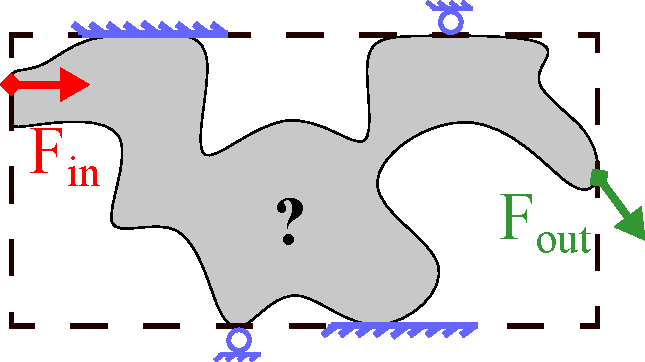
\includegraphics[width=0.5\columnwidth]{images/chap5/TOM-wp.pdf}
    \caption{Basic design problem for compliant mechanisms.}
    \label{fig:ComplProb}
\end{figure}

\subsection{Density-Based Topology Optimization}
The basic concept being topology optimisation consists of investigating the distribution of material inside a discretised design space while trying to improve a certain specified objective function. The design variables applied in this density-based approach optimisation are artificial densities $\ArtDen$ that describe the proportion of the material, $0<\ArtDen_\text{min} \leq \ArtDen \leq 1$, an individual domain space is filled with. The lower and upper bounds of density range are considered as \textit{full} materials representing fully empty or fully filled elements, respectively. While the densities within the range are defined as \textit{intermediate} materials. Here, this artificial density variable are made continuous to use a gradient-based solver which has the advantage of lower computational time compared to non-gradient based approaches, as shown in the work by \cite{sigmundUsefulnessNongradientApproaches2011}. In order to avoid mesh-dependent solutions and checker-board patters, the optimisation is regulated. This is achieved with a density filter that limits the length scale, $\FiltRadius$, to a minimum inside the structure, as shown in the work by \cite{bendsoeTopologyOptimizationTheory2013}.

Each iteration of the optimisation consists of the following steps. First, the filtered design variables are mapped to a material property using the Material Interpolation Scheme (MIS). This converts the artificial densities into a usable Young's Modulus. Next, the well-known Solid Isotropic Material Penalisation (SIMP), as shown in \cref{eq:SIMP} from the work by \cite{bendsoeTopologyOptimizationTheory2013}, is implemented. This scheme penalises intermediate materials so as to prevent obtaining a geometry that cannot be manufactured. This is done using a penalty facor $\PenFac$ which continuously increases throughout the optimisation.
\begin{equation} % MIS SIMP
  \YoungModulus_\elem = \MIS(\ArtDen_\elem) = ( \overline{\YoungModulus} - \underline{\YoungModulus} ) \ArtDen_\elem ^\PenFac + \underline{\YoungModulus},
\label{eq:SIMP}
\end{equation}
with $\underline{\YoungModulus}$, $\overline{\YoungModulus}$ the lower and upper bound of $\vec{\YoungModulus} =  [\ \!\! \YoungModulus, \cdots, \YoungModulus_\NDesElem]\ \!\!^\text{T}$ respectively corresponding to the Young's modulus of an "empty" element and a completely filled one. $\NDesElem$ is the number of elements inside the domain.
When the material properties of each element are known, the \textit{Stiffness matrix} $\StiffMat$ of the corresponding structure is constructed. Next, Finite Element Analysis (FEA) is performed to estimate the displacement $\Disp$ of each node under imposed external loads $\Load$ so as to solve the linear elasticity equation: $\StiffMat \Disp = \Load$. The chosen objective function with its associated sensitivity (gradient of the objective function with respect to the design variable) is evaluated using these, aforementioned, displacements. For the following iteration, the sensitivities can, then, be used by the solver to update the design variables. In this case, the Optimality Criteria (OC) scheme from the work by \cite{bendsoeTopologyOptimizationTheory2013} is used as the solver.

One of the main advantages to this approach to designing compliant SMA elements is the fact that various Open-Source academic codes are available for implementing this structural topology optimisation as shown in the work by \cite{zhuDesignCompliantMechanisms2020} and \cite{talischiPolyTopMatlabImplementation2012}. Due to ignoring the thermal dependencies of the shape memory effect, the resulting FEA used is similar to that of traditional compliant mechanisms and can thus be easily extended to such generative algorithms by simply changing the objective functions and associated sensitivity.

\subsection{Topology Optimization of Compliant Mechanisms}
The basic principle behind designing a compliant mechanism, as illustrated in \cref{fig:ComplProb}, can be formulated as : "Under an external input force and certain boundary conditions, what is the distribution of material defining the compliant mechanism that transforms the input load to a specific output one?"

At the input and output points, artificial springs are added to simulate the input work and resistance to the output displacement of the workpiece, respectively, as shown in the work by \cite{alonsoTopologySynthesisMultiInput2014}. In the final geometry, these springs are removed and are only present during the design process. Regarding the objective function that governs the final design of the compliant mechanism, a formulation that can be extended to Multi-Input Multi-Outputs (MIMO), is implemented based on various strain energies as shown in the work by \cite{alonsoTopologySynthesisMultiInput2014}.

An objective function based upon the mutual strain energy between the input and output is chosen. This permits to distribute the strain throughout the structure and avoid to have only \textit{de facto} (single point) hinges responsible for the compliant behaviour. Ideally, the maximum volume of the structure should be deformed to harvest as maximum work, when the alloy is heated and experiences the shape memory effect. Here, the objective function is built using three different types of strain energies. First, there is the input strain energy $\EStrain_\text{in}$, that is present when only an input load $\Load_\text{in}$ is applied and result in some nodal displacements $\Disp_\text{in}$. Similarly, the output strain energy $\EStrain_\text{out}$, is present when only a dummy unit load $\Load_\text{out}$ is applied at the output port resulting in nodal displacements $\Disp_\text{out}$. Finally, the Mutual Potential Energy (MPE) or mutual strain energy $\EStrain_\text{mut}$ can be built with the two previous nodal displacements. The objective function is chosen as a ratio of these three energies due to its non-dimensional aspect and due to the fact that the desired input and output displacements are indirectly accounted for. Here, since the problem is formulated as a minimisation, a minus signed is placed before the chosen ratio to maximise the MPE as follows :
\begin{equation}
    \ObjFct = - \frac{\EStrain_\text{mut}}{\EStrain_\text{in} + \EStrain_\text{out}} = -\frac{{\Disp _\text{out}}^\text{T} \StiffMat \Disp_\text{int}}{\frac{1}{2} {\Disp_\text{out}}^\text{T} \StiffMat \Disp_\text{out} + \frac{1}{2} {\Disp_\text{in}}^\text{T} \StiffMat \Disp_\text{in}}.
\end{equation}
Lastly, two separate FEAs are performed to evaluate the chosen objective: $\StiffMat \Disp_\text{in} = \Load_\text{in}$ and  $\StiffMat \Disp_\text{out} = \Load_\text{out}$.

The current objective governing the design of the generated compliant mechanisms made of \textit{conventional} linear material, can be extended to generating design for mechanisms made from SMAs. This is due to the fact that, as previously mentioned, the algorithm tends to distribute the strain throughout the structure which will indirectly allow a large portion of the material to be activated if made from SMA. The optimisation problem, as formulated in \cref{eq:OptProblem}, consists of the minimisation of the objective function $\ObjFct$ subject to the limitation of the infill $\Volume^{\ast}$ of the design domain's volume, with $\VolumeElem_\elem$ the volume of element $\elem$.

\begin{alignat}{2} % Optimization problem
  \label{eq:OptProblem}
  &\underset{\vec{\ArtDen}}{\text{min}} : \quad        &&\ObjFct(\vec{\Disp_\text{in}},\vec{\Disp_\text{out}},\vec{\YoungModulus}) \notag \\
  &\text{s.t. :}            &&  \StiffMat \Disp_\text{in} = \Load_\text{in}         \notag       \\
  &                         &&  \StiffMat \Disp_\text{out} = \Load_\text{out}                \\
  &                         && \Volume < \Volume^{\ast} \text{,   with } \Volume = (\sum_{\elem=1}^{\NDesElem} \ArtDen_\elem \cdot \VolumeElem_\elem) / (\sum_{\elem=1}^{\NDesElem} \VolumeElem_\elem)   \notag      \\
  &                         && \vec{\YoungModulus} = \MIS(\vec{\ArtDen})    \quad \;     0<\ArtDen_\text{min}    \leqslant \ArtDen    \leqslant 1.     \notag
\end{alignat}

In \cref{fig:Invert_ProbFinal}, the basic design problem is displayed using the common force inverter scenario. Due to the symmetry of the problem, the domain space can be restricted to half the surface while adding rolling supports at the symmetry axis. In \cref{fig:ForceInverter_evol}, the evolution of the optimisation can be observed. Here the domain space is uniformly initialised with intermediate materials such that the volume limitation is satisfied so as to have the design converge to a solution that is only composed of full materials.

\section{Testing using Benchmark problems}\label{sec:benchmark-problems}
Before designing complex multi-output compliant SMA elements, the shape memory effect of the generated geometries must be validated. In this regard, a common practice is to use some traditional benchmark problems. The problems, while being simple problems, can be used to validate the generated designs using a commercially available Finite Element Modelling (FEM) software such as ANSYS\textsuperscript{\textregistered}. Using an FEM, the shape memory effect of the generated topologies can be simulated, verifying the efficiency of the algorithm for designing compliant SMA mechanisms.

The proposed design method is applied to three benchmark problems : an inverter, a crimper, and a gripper. They are all fixed at their bottom and top left corners (which corresponds to ideal pivots) but each have their own input and output forces. The design problems and the resulting geometries are shown in \cref{fig:Invert_ProbFinal}, \cref{fig:Crimper_ProbFinal}, and \cref{fig:Gripper_ProbFinal}. This half domain space has been discretised into $10^4$ elements and the design variables are initialised uniformly with a volume fraction constraint of 30\%. The stiffness of each artificial spring is equal to 0.1 and the input forces are equal to 1. When run on a Windows workstation with an Intel i7 3.6 GHz, 8-core processor and 32 GB of memory, the complete process takes less than 1 minute to converge to solution. It is important to note that the computational time would have been significantly higher if a non-linear and multi-physic analysis was executed. Due to the short computational time, this design method can be extended to 3-Dimensional problems.

\begin{figure}[hbt!]
    \centering
    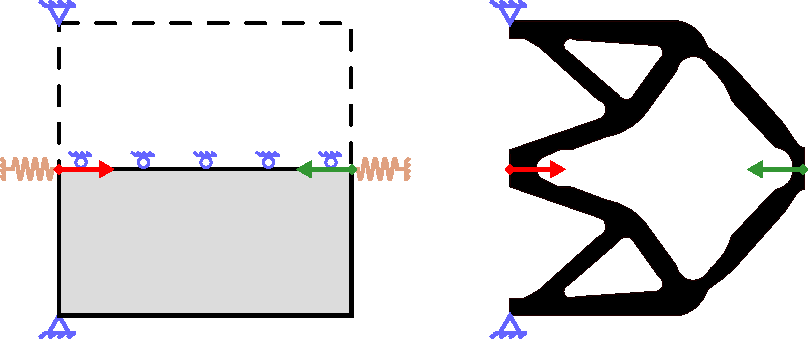
\includegraphics[width=0.65\columnwidth]{images/chap5/Inverter_Schematic_FinalCAD.pdf}
    \caption{Inverter: Design problem (left), Interpolated final topology (right). Input force is shown in red while the output force is shown green.}
    \label{fig:Invert_ProbFinal}
\end{figure}

\begin{figure}[hbt!]
    \centering
     \begin{subfigure}[t]{0.24\columnwidth} % The width should be scaled to the desired one depending on the number and sizes of sub-figures
     \centering
		   
\includegraphics[width=\textwidth]{images/chap5/Inverter_evo_00.png} % the textwidth will correspond to the one provide by the subfigure width
    %  \caption{Initial}
 \end{subfigure}
%  \hspace{0.2cm}
%  \begin{subfigure}[t]{0.24\columnwidth} % the [t] extension aligns the figure with their tops
%      \centering
% 		   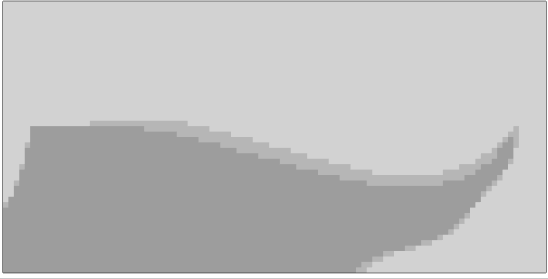
\includegraphics[width=\textwidth]{Inverter_evo_01.png} % the textwidth will correspond to the one provide by the subfigure width
%     %  \caption{Iteration 2}
%  \end{subfigure}
 \hspace{0.2cm}
 \begin{subfigure}[t]{0.24\columnwidth} % the [t] extension aligns the figure with their tops
     \centering
		   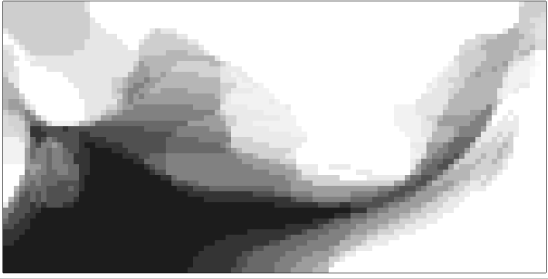
\includegraphics[width=\textwidth]{images/chap5/Inverter_evo_02.png} % the textwidth will correspond to the one provide by the subfigure width
    %  \caption{Iteration 8}
 \end{subfigure}
 \hspace{0.2cm}
 \begin{subfigure}[t]{0.24\columnwidth} % the [t] extension aligns the figure with their tops
     \centering
		   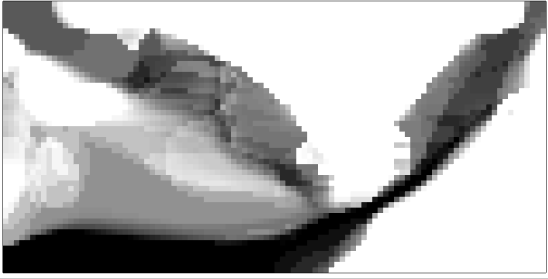
\includegraphics[width=\textwidth]{images/chap5/Inverter_evo_03.png} % the textwidth will correspond to the one provide by the subfigure width
    %  \caption{Iteration 21}
 \end{subfigure}
 \medbreak
 \begin{subfigure}[t]{0.24\columnwidth} % the [t] extension aligns the figure with their tops
     \centering
		   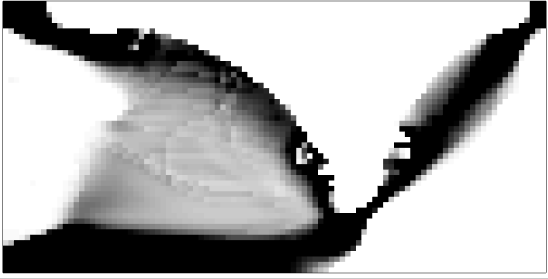
\includegraphics[width=\textwidth]{images/chap5/Inverter_evo_04.png} % the textwidth will correspond to the one provide by the subfigure width
    %  \caption{Iteration 57}
 \end{subfigure}
 \hspace{0.2cm}
 \begin{subfigure}[t]{0.25\columnwidth} % the [t] extension aligns the figure with their tops
     \centering
		   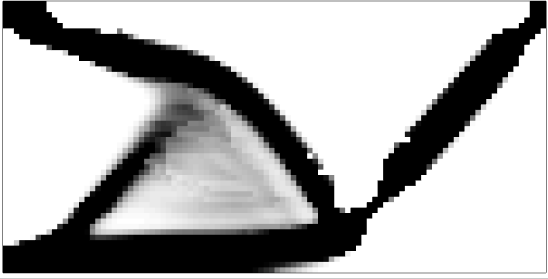
\includegraphics[width=\textwidth]{images/chap5/Inverter_evo_05.png} % the textwidth will correspond to the one provide by the subfigure width
    %  \caption{Iteration 98}
 \end{subfigure}
  \hspace{0.2cm}
 \begin{subfigure}[t]{0.25\columnwidth} % the [t] extension aligns the figure with their tops
     \centering
		   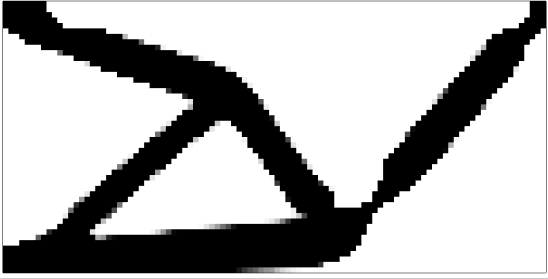
\includegraphics[width=\textwidth]{images/chap5/Inverter_evo_final.png} % the textwidth will correspond to the one provide by the subfigure width
    %  \caption{Iteration 133}
 \end{subfigure}

    \caption{Evolution of the inverter design throughout the optimization. The grayscale represent the value of the filtered artificial density.}
    \label{fig:ForceInverter_evol}
\end{figure}

\begin{figure}[hbt!]
    \centering
    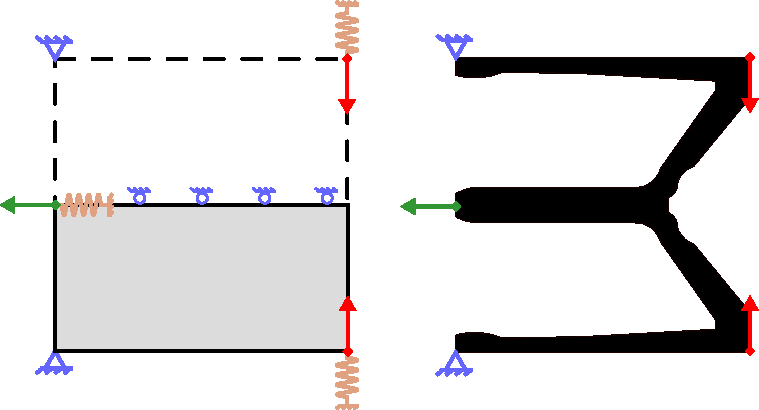
\includegraphics[width=0.65\columnwidth]{images/chap5/Crimper_Schematic_FinalCAD.pdf}
    \caption{Crimper: Design problem (left), Interpolated final topology (right). Input force is shown in red while the output force is shown green.}
    \label{fig:Crimper_ProbFinal}
\end{figure}
\begin{figure}[hbt!]
    \centering
    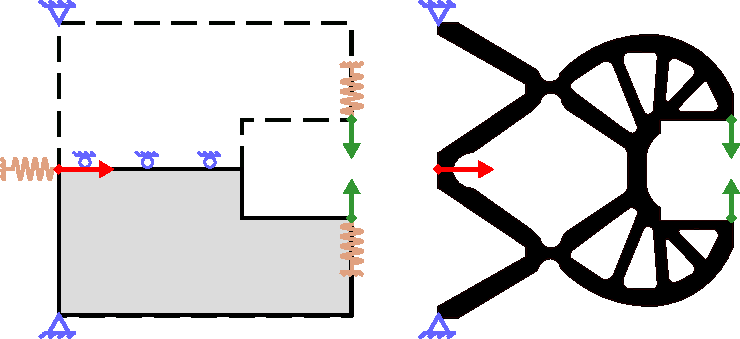
\includegraphics[width=0.65\columnwidth]{images/chap5/Gripper_Schematic_FinalCAD.pdf}
    \caption{Gripper: Design problem (left), Interpolated final topology (right). Input force is shown in red while the output force is shown green.}
    \label{fig:Gripper_ProbFinal}
\end{figure}

Here, in the hopes of validating the shape memory effect, a four time-step simulation is constructed. The four different simulated steps can be seen in \cref{fig:InverterAnsysSimu}. Here, the figures represent the results of the FEM simulation for each benchmark problem. The simulation consists of first applying an input displacement which generates a displacement at the output, $\varepsilon_\text{loaded}$. If the entire structure is sufficiently strained to undergo the detwinning process, as explained in chapter \todocite, the structure will keep its deformed shape when the input displacement constraint is released. However, as some areas of the compliant structure does not undergo detwinning, a portion of the strain will be lost when the constraint is released. Thus, the observed strain at the output will decrease to $\varepsilon_\text{free}$. During the third time step, the structure is heated to activate the shape memory effect and force the structure to revert back to its original shape where all the strain is recovered. Finally, the structure is allowed to cool down and return the material back to its martensitic phase.

\begin{figure}[hbt!]
    \centering
    % !TEX root = ../sethomas_thesis_main.tex
\documentclass[border=1mm,
               class=article
               preview]{standalone}
\usepackage{tikz}
\begin{document}
\begin{tikzpicture}
    \node[anchor=south west,inner sep=0] (graph) at (0,0) {\resizebox{\columnwidth}{!}{%% Creator: Matplotlib, PGF backend
%%
%% To include the figure in your LaTeX document, write
%%   \input{<filename>.pgf}
%%
%% Make sure the required packages are loaded in your preamble
%%   \usepackage{pgf}
%%
%% and, on pdftex
%%   \usepackage[utf8]{inputenc}\DeclareUnicodeCharacter{2212}{-}
%%
%% or, on luatex and xetex
%%   \usepackage{unicode-math}
%%
%% Figures using additional raster images can only be included by \input if
%% they are in the same directory as the main LaTeX file. For loading figures
%% from other directories you can use the `import` package
%%   \usepackage{import}
%%
%% and then include the figures with
%%   \import{<path to file>}{<filename>.pgf}
%%
%% Matplotlib used the following preamble
%%
\begingroup%
\makeatletter%
\begin{pgfpicture}%
\pgfpathrectangle{\pgfpointorigin}{\pgfqpoint{8.602007in}{4.649344in}}%
\pgfusepath{use as bounding box, clip}%
\begin{pgfscope}%
\pgfsetbuttcap%
\pgfsetmiterjoin%
\pgfsetlinewidth{0.000000pt}%
\definecolor{currentstroke}{rgb}{0.000000,0.000000,0.000000}%
\pgfsetstrokecolor{currentstroke}%
\pgfsetstrokeopacity{0.000000}%
\pgfsetdash{}{0pt}%
\pgfpathmoveto{\pgfqpoint{0.000000in}{0.000000in}}%
\pgfpathlineto{\pgfqpoint{8.602007in}{0.000000in}}%
\pgfpathlineto{\pgfqpoint{8.602007in}{4.649344in}}%
\pgfpathlineto{\pgfqpoint{0.000000in}{4.649344in}}%
\pgfpathclose%
\pgfusepath{}%
\end{pgfscope}%
\begin{pgfscope}%
\pgfsetbuttcap%
\pgfsetmiterjoin%
\pgfsetlinewidth{0.000000pt}%
\definecolor{currentstroke}{rgb}{0.000000,0.000000,0.000000}%
\pgfsetstrokecolor{currentstroke}%
\pgfsetstrokeopacity{0.000000}%
\pgfsetdash{}{0pt}%
\pgfpathmoveto{\pgfqpoint{0.717284in}{3.271659in}}%
\pgfpathlineto{\pgfqpoint{8.467284in}{3.271659in}}%
\pgfpathlineto{\pgfqpoint{8.467284in}{4.404012in}}%
\pgfpathlineto{\pgfqpoint{0.717284in}{4.404012in}}%
\pgfpathclose%
\pgfusepath{}%
\end{pgfscope}%
\begin{pgfscope}%
\pgfpathrectangle{\pgfqpoint{0.717284in}{3.271659in}}{\pgfqpoint{7.750000in}{1.132353in}}%
\pgfusepath{clip}%
\pgfsetbuttcap%
\pgfsetroundjoin%
\pgfsetlinewidth{0.803000pt}%
\definecolor{currentstroke}{rgb}{0.690196,0.690196,0.690196}%
\pgfsetstrokecolor{currentstroke}%
\pgfsetdash{{2.960000pt}{1.280000pt}}{0.000000pt}%
\pgfpathmoveto{\pgfqpoint{2.654784in}{3.271659in}}%
\pgfpathlineto{\pgfqpoint{2.654784in}{4.404012in}}%
\pgfusepath{stroke}%
\end{pgfscope}%
\begin{pgfscope}%
\pgfsetbuttcap%
\pgfsetroundjoin%
\definecolor{currentfill}{rgb}{0.000000,0.000000,0.000000}%
\pgfsetfillcolor{currentfill}%
\pgfsetlinewidth{0.803000pt}%
\definecolor{currentstroke}{rgb}{0.000000,0.000000,0.000000}%
\pgfsetstrokecolor{currentstroke}%
\pgfsetdash{}{0pt}%
\pgfsys@defobject{currentmarker}{\pgfqpoint{0.000000in}{-0.048611in}}{\pgfqpoint{0.000000in}{0.000000in}}{%
\pgfpathmoveto{\pgfqpoint{0.000000in}{0.000000in}}%
\pgfpathlineto{\pgfqpoint{0.000000in}{-0.048611in}}%
\pgfusepath{stroke,fill}%
}%
\begin{pgfscope}%
\pgfsys@transformshift{2.654784in}{3.271659in}%
\pgfsys@useobject{currentmarker}{}%
\end{pgfscope}%
\end{pgfscope}%
\begin{pgfscope}%
\pgfpathrectangle{\pgfqpoint{0.717284in}{3.271659in}}{\pgfqpoint{7.750000in}{1.132353in}}%
\pgfusepath{clip}%
\pgfsetbuttcap%
\pgfsetroundjoin%
\pgfsetlinewidth{0.803000pt}%
\definecolor{currentstroke}{rgb}{0.690196,0.690196,0.690196}%
\pgfsetstrokecolor{currentstroke}%
\pgfsetdash{{2.960000pt}{1.280000pt}}{0.000000pt}%
\pgfpathmoveto{\pgfqpoint{4.592284in}{3.271659in}}%
\pgfpathlineto{\pgfqpoint{4.592284in}{4.404012in}}%
\pgfusepath{stroke}%
\end{pgfscope}%
\begin{pgfscope}%
\pgfsetbuttcap%
\pgfsetroundjoin%
\definecolor{currentfill}{rgb}{0.000000,0.000000,0.000000}%
\pgfsetfillcolor{currentfill}%
\pgfsetlinewidth{0.803000pt}%
\definecolor{currentstroke}{rgb}{0.000000,0.000000,0.000000}%
\pgfsetstrokecolor{currentstroke}%
\pgfsetdash{}{0pt}%
\pgfsys@defobject{currentmarker}{\pgfqpoint{0.000000in}{-0.048611in}}{\pgfqpoint{0.000000in}{0.000000in}}{%
\pgfpathmoveto{\pgfqpoint{0.000000in}{0.000000in}}%
\pgfpathlineto{\pgfqpoint{0.000000in}{-0.048611in}}%
\pgfusepath{stroke,fill}%
}%
\begin{pgfscope}%
\pgfsys@transformshift{4.592284in}{3.271659in}%
\pgfsys@useobject{currentmarker}{}%
\end{pgfscope}%
\end{pgfscope}%
\begin{pgfscope}%
\pgfpathrectangle{\pgfqpoint{0.717284in}{3.271659in}}{\pgfqpoint{7.750000in}{1.132353in}}%
\pgfusepath{clip}%
\pgfsetbuttcap%
\pgfsetroundjoin%
\pgfsetlinewidth{0.803000pt}%
\definecolor{currentstroke}{rgb}{0.690196,0.690196,0.690196}%
\pgfsetstrokecolor{currentstroke}%
\pgfsetdash{{2.960000pt}{1.280000pt}}{0.000000pt}%
\pgfpathmoveto{\pgfqpoint{6.529784in}{3.271659in}}%
\pgfpathlineto{\pgfqpoint{6.529784in}{4.404012in}}%
\pgfusepath{stroke}%
\end{pgfscope}%
\begin{pgfscope}%
\pgfsetbuttcap%
\pgfsetroundjoin%
\definecolor{currentfill}{rgb}{0.000000,0.000000,0.000000}%
\pgfsetfillcolor{currentfill}%
\pgfsetlinewidth{0.803000pt}%
\definecolor{currentstroke}{rgb}{0.000000,0.000000,0.000000}%
\pgfsetstrokecolor{currentstroke}%
\pgfsetdash{}{0pt}%
\pgfsys@defobject{currentmarker}{\pgfqpoint{0.000000in}{-0.048611in}}{\pgfqpoint{0.000000in}{0.000000in}}{%
\pgfpathmoveto{\pgfqpoint{0.000000in}{0.000000in}}%
\pgfpathlineto{\pgfqpoint{0.000000in}{-0.048611in}}%
\pgfusepath{stroke,fill}%
}%
\begin{pgfscope}%
\pgfsys@transformshift{6.529784in}{3.271659in}%
\pgfsys@useobject{currentmarker}{}%
\end{pgfscope}%
\end{pgfscope}%
\begin{pgfscope}%
\pgfpathrectangle{\pgfqpoint{0.717284in}{3.271659in}}{\pgfqpoint{7.750000in}{1.132353in}}%
\pgfusepath{clip}%
\pgfsetbuttcap%
\pgfsetroundjoin%
\pgfsetlinewidth{0.803000pt}%
\definecolor{currentstroke}{rgb}{0.690196,0.690196,0.690196}%
\pgfsetstrokecolor{currentstroke}%
\pgfsetdash{{2.960000pt}{1.280000pt}}{0.000000pt}%
\pgfpathmoveto{\pgfqpoint{8.467284in}{3.271659in}}%
\pgfpathlineto{\pgfqpoint{8.467284in}{4.404012in}}%
\pgfusepath{stroke}%
\end{pgfscope}%
\begin{pgfscope}%
\pgfsetbuttcap%
\pgfsetroundjoin%
\definecolor{currentfill}{rgb}{0.000000,0.000000,0.000000}%
\pgfsetfillcolor{currentfill}%
\pgfsetlinewidth{0.803000pt}%
\definecolor{currentstroke}{rgb}{0.000000,0.000000,0.000000}%
\pgfsetstrokecolor{currentstroke}%
\pgfsetdash{}{0pt}%
\pgfsys@defobject{currentmarker}{\pgfqpoint{0.000000in}{-0.048611in}}{\pgfqpoint{0.000000in}{0.000000in}}{%
\pgfpathmoveto{\pgfqpoint{0.000000in}{0.000000in}}%
\pgfpathlineto{\pgfqpoint{0.000000in}{-0.048611in}}%
\pgfusepath{stroke,fill}%
}%
\begin{pgfscope}%
\pgfsys@transformshift{8.467284in}{3.271659in}%
\pgfsys@useobject{currentmarker}{}%
\end{pgfscope}%
\end{pgfscope}%
\begin{pgfscope}%
\pgfpathrectangle{\pgfqpoint{0.717284in}{3.271659in}}{\pgfqpoint{7.750000in}{1.132353in}}%
\pgfusepath{clip}%
\pgfsetbuttcap%
\pgfsetroundjoin%
\pgfsetlinewidth{0.803000pt}%
\definecolor{currentstroke}{rgb}{0.690196,0.690196,0.690196}%
\pgfsetstrokecolor{currentstroke}%
\pgfsetdash{{2.960000pt}{1.280000pt}}{0.000000pt}%
\pgfpathmoveto{\pgfqpoint{0.717284in}{3.323129in}}%
\pgfpathlineto{\pgfqpoint{8.467284in}{3.323129in}}%
\pgfusepath{stroke}%
\end{pgfscope}%
\begin{pgfscope}%
\pgfsetbuttcap%
\pgfsetroundjoin%
\definecolor{currentfill}{rgb}{0.000000,0.000000,0.000000}%
\pgfsetfillcolor{currentfill}%
\pgfsetlinewidth{0.803000pt}%
\definecolor{currentstroke}{rgb}{0.000000,0.000000,0.000000}%
\pgfsetstrokecolor{currentstroke}%
\pgfsetdash{}{0pt}%
\pgfsys@defobject{currentmarker}{\pgfqpoint{-0.048611in}{0.000000in}}{\pgfqpoint{-0.000000in}{0.000000in}}{%
\pgfpathmoveto{\pgfqpoint{-0.000000in}{0.000000in}}%
\pgfpathlineto{\pgfqpoint{-0.048611in}{0.000000in}}%
\pgfusepath{stroke,fill}%
}%
\begin{pgfscope}%
\pgfsys@transformshift{0.717284in}{3.323129in}%
\pgfsys@useobject{currentmarker}{}%
\end{pgfscope}%
\end{pgfscope}%
\begin{pgfscope}%
\definecolor{textcolor}{rgb}{0.000000,0.000000,0.000000}%
\pgfsetstrokecolor{textcolor}%
\pgfsetfillcolor{textcolor}%
\pgftext[x=0.481173in, y=3.274904in, left, base]{\color{textcolor}\rmfamily\fontsize{10.000000}{12.000000}\selectfont \(\displaystyle {22}\)}%
\end{pgfscope}%
\begin{pgfscope}%
\pgfpathrectangle{\pgfqpoint{0.717284in}{3.271659in}}{\pgfqpoint{7.750000in}{1.132353in}}%
\pgfusepath{clip}%
\pgfsetbuttcap%
\pgfsetroundjoin%
\pgfsetlinewidth{0.803000pt}%
\definecolor{currentstroke}{rgb}{0.690196,0.690196,0.690196}%
\pgfsetstrokecolor{currentstroke}%
\pgfsetdash{{2.960000pt}{1.280000pt}}{0.000000pt}%
\pgfpathmoveto{\pgfqpoint{0.717284in}{4.352541in}}%
\pgfpathlineto{\pgfqpoint{8.467284in}{4.352541in}}%
\pgfusepath{stroke}%
\end{pgfscope}%
\begin{pgfscope}%
\pgfsetbuttcap%
\pgfsetroundjoin%
\definecolor{currentfill}{rgb}{0.000000,0.000000,0.000000}%
\pgfsetfillcolor{currentfill}%
\pgfsetlinewidth{0.803000pt}%
\definecolor{currentstroke}{rgb}{0.000000,0.000000,0.000000}%
\pgfsetstrokecolor{currentstroke}%
\pgfsetdash{}{0pt}%
\pgfsys@defobject{currentmarker}{\pgfqpoint{-0.048611in}{0.000000in}}{\pgfqpoint{-0.000000in}{0.000000in}}{%
\pgfpathmoveto{\pgfqpoint{-0.000000in}{0.000000in}}%
\pgfpathlineto{\pgfqpoint{-0.048611in}{0.000000in}}%
\pgfusepath{stroke,fill}%
}%
\begin{pgfscope}%
\pgfsys@transformshift{0.717284in}{4.352541in}%
\pgfsys@useobject{currentmarker}{}%
\end{pgfscope}%
\end{pgfscope}%
\begin{pgfscope}%
\definecolor{textcolor}{rgb}{0.000000,0.000000,0.000000}%
\pgfsetstrokecolor{textcolor}%
\pgfsetfillcolor{textcolor}%
\pgftext[x=0.411728in, y=4.304316in, left, base]{\color{textcolor}\rmfamily\fontsize{10.000000}{12.000000}\selectfont \(\displaystyle {160}\)}%
\end{pgfscope}%
\begin{pgfscope}%
\definecolor{textcolor}{rgb}{0.000000,0.000000,0.000000}%
\pgfsetstrokecolor{textcolor}%
\pgfsetfillcolor{textcolor}%
\pgftext[x=0.356173in,y=3.837835in,,bottom,rotate=90.000000]{\color{textcolor}\rmfamily\fontsize{12.000000}{14.400000}\bfseries\selectfont Temperature [°C]}%
\end{pgfscope}%
\begin{pgfscope}%
\pgfpathrectangle{\pgfqpoint{0.717284in}{3.271659in}}{\pgfqpoint{7.750000in}{1.132353in}}%
\pgfusepath{clip}%
\pgfsetbuttcap%
\pgfsetroundjoin%
\pgfsetlinewidth{3.011250pt}%
\definecolor{currentstroke}{rgb}{0.450980,0.670588,1.000000}%
\pgfsetstrokecolor{currentstroke}%
\pgfsetdash{{3.000000pt}{4.950000pt}}{0.000000pt}%
\pgfpathmoveto{\pgfqpoint{0.717284in}{3.323129in}}%
\pgfpathlineto{\pgfqpoint{4.592284in}{3.323129in}}%
\pgfpathlineto{\pgfqpoint{5.754978in}{3.940851in}}%
\pgfpathlineto{\pgfqpoint{5.756722in}{3.941000in}}%
\pgfpathlineto{\pgfqpoint{6.529784in}{4.352541in}}%
\pgfpathlineto{\pgfqpoint{6.529784in}{4.352541in}}%
\pgfpathlineto{\pgfqpoint{8.467284in}{3.323129in}}%
\pgfpathlineto{\pgfqpoint{8.467284in}{3.323129in}}%
\pgfusepath{stroke}%
\end{pgfscope}%
\begin{pgfscope}%
\pgfsetrectcap%
\pgfsetmiterjoin%
\pgfsetlinewidth{0.803000pt}%
\definecolor{currentstroke}{rgb}{0.000000,0.000000,0.000000}%
\pgfsetstrokecolor{currentstroke}%
\pgfsetdash{}{0pt}%
\pgfpathmoveto{\pgfqpoint{0.717284in}{3.271659in}}%
\pgfpathlineto{\pgfqpoint{0.717284in}{4.404012in}}%
\pgfusepath{stroke}%
\end{pgfscope}%
\begin{pgfscope}%
\pgfsetrectcap%
\pgfsetmiterjoin%
\pgfsetlinewidth{0.803000pt}%
\definecolor{currentstroke}{rgb}{0.000000,0.000000,0.000000}%
\pgfsetstrokecolor{currentstroke}%
\pgfsetdash{}{0pt}%
\pgfpathmoveto{\pgfqpoint{8.467284in}{3.271659in}}%
\pgfpathlineto{\pgfqpoint{8.467284in}{4.404012in}}%
\pgfusepath{stroke}%
\end{pgfscope}%
\begin{pgfscope}%
\pgfsetrectcap%
\pgfsetmiterjoin%
\pgfsetlinewidth{0.803000pt}%
\definecolor{currentstroke}{rgb}{0.000000,0.000000,0.000000}%
\pgfsetstrokecolor{currentstroke}%
\pgfsetdash{}{0pt}%
\pgfpathmoveto{\pgfqpoint{0.717284in}{3.271659in}}%
\pgfpathlineto{\pgfqpoint{8.467284in}{3.271659in}}%
\pgfusepath{stroke}%
\end{pgfscope}%
\begin{pgfscope}%
\pgfsetrectcap%
\pgfsetmiterjoin%
\pgfsetlinewidth{0.803000pt}%
\definecolor{currentstroke}{rgb}{0.000000,0.000000,0.000000}%
\pgfsetstrokecolor{currentstroke}%
\pgfsetdash{}{0pt}%
\pgfpathmoveto{\pgfqpoint{0.717284in}{4.404012in}}%
\pgfpathlineto{\pgfqpoint{8.467284in}{4.404012in}}%
\pgfusepath{stroke}%
\end{pgfscope}%
\begin{pgfscope}%
\pgfsetbuttcap%
\pgfsetmiterjoin%
\pgfsetlinewidth{0.000000pt}%
\definecolor{currentstroke}{rgb}{0.000000,0.000000,0.000000}%
\pgfsetstrokecolor{currentstroke}%
\pgfsetstrokeopacity{0.000000}%
\pgfsetdash{}{0pt}%
\pgfpathmoveto{\pgfqpoint{0.717284in}{1.912835in}}%
\pgfpathlineto{\pgfqpoint{8.467284in}{1.912835in}}%
\pgfpathlineto{\pgfqpoint{8.467284in}{3.045188in}}%
\pgfpathlineto{\pgfqpoint{0.717284in}{3.045188in}}%
\pgfpathclose%
\pgfusepath{}%
\end{pgfscope}%
\begin{pgfscope}%
\pgfpathrectangle{\pgfqpoint{0.717284in}{1.912835in}}{\pgfqpoint{7.750000in}{1.132353in}}%
\pgfusepath{clip}%
\pgfsetbuttcap%
\pgfsetroundjoin%
\pgfsetlinewidth{0.803000pt}%
\definecolor{currentstroke}{rgb}{0.690196,0.690196,0.690196}%
\pgfsetstrokecolor{currentstroke}%
\pgfsetdash{{2.960000pt}{1.280000pt}}{0.000000pt}%
\pgfpathmoveto{\pgfqpoint{2.654784in}{1.912835in}}%
\pgfpathlineto{\pgfqpoint{2.654784in}{3.045188in}}%
\pgfusepath{stroke}%
\end{pgfscope}%
\begin{pgfscope}%
\pgfsetbuttcap%
\pgfsetroundjoin%
\definecolor{currentfill}{rgb}{0.000000,0.000000,0.000000}%
\pgfsetfillcolor{currentfill}%
\pgfsetlinewidth{0.803000pt}%
\definecolor{currentstroke}{rgb}{0.000000,0.000000,0.000000}%
\pgfsetstrokecolor{currentstroke}%
\pgfsetdash{}{0pt}%
\pgfsys@defobject{currentmarker}{\pgfqpoint{0.000000in}{-0.048611in}}{\pgfqpoint{0.000000in}{0.000000in}}{%
\pgfpathmoveto{\pgfqpoint{0.000000in}{0.000000in}}%
\pgfpathlineto{\pgfqpoint{0.000000in}{-0.048611in}}%
\pgfusepath{stroke,fill}%
}%
\begin{pgfscope}%
\pgfsys@transformshift{2.654784in}{1.912835in}%
\pgfsys@useobject{currentmarker}{}%
\end{pgfscope}%
\end{pgfscope}%
\begin{pgfscope}%
\pgfpathrectangle{\pgfqpoint{0.717284in}{1.912835in}}{\pgfqpoint{7.750000in}{1.132353in}}%
\pgfusepath{clip}%
\pgfsetbuttcap%
\pgfsetroundjoin%
\pgfsetlinewidth{0.803000pt}%
\definecolor{currentstroke}{rgb}{0.690196,0.690196,0.690196}%
\pgfsetstrokecolor{currentstroke}%
\pgfsetdash{{2.960000pt}{1.280000pt}}{0.000000pt}%
\pgfpathmoveto{\pgfqpoint{4.592284in}{1.912835in}}%
\pgfpathlineto{\pgfqpoint{4.592284in}{3.045188in}}%
\pgfusepath{stroke}%
\end{pgfscope}%
\begin{pgfscope}%
\pgfsetbuttcap%
\pgfsetroundjoin%
\definecolor{currentfill}{rgb}{0.000000,0.000000,0.000000}%
\pgfsetfillcolor{currentfill}%
\pgfsetlinewidth{0.803000pt}%
\definecolor{currentstroke}{rgb}{0.000000,0.000000,0.000000}%
\pgfsetstrokecolor{currentstroke}%
\pgfsetdash{}{0pt}%
\pgfsys@defobject{currentmarker}{\pgfqpoint{0.000000in}{-0.048611in}}{\pgfqpoint{0.000000in}{0.000000in}}{%
\pgfpathmoveto{\pgfqpoint{0.000000in}{0.000000in}}%
\pgfpathlineto{\pgfqpoint{0.000000in}{-0.048611in}}%
\pgfusepath{stroke,fill}%
}%
\begin{pgfscope}%
\pgfsys@transformshift{4.592284in}{1.912835in}%
\pgfsys@useobject{currentmarker}{}%
\end{pgfscope}%
\end{pgfscope}%
\begin{pgfscope}%
\pgfpathrectangle{\pgfqpoint{0.717284in}{1.912835in}}{\pgfqpoint{7.750000in}{1.132353in}}%
\pgfusepath{clip}%
\pgfsetbuttcap%
\pgfsetroundjoin%
\pgfsetlinewidth{0.803000pt}%
\definecolor{currentstroke}{rgb}{0.690196,0.690196,0.690196}%
\pgfsetstrokecolor{currentstroke}%
\pgfsetdash{{2.960000pt}{1.280000pt}}{0.000000pt}%
\pgfpathmoveto{\pgfqpoint{6.529784in}{1.912835in}}%
\pgfpathlineto{\pgfqpoint{6.529784in}{3.045188in}}%
\pgfusepath{stroke}%
\end{pgfscope}%
\begin{pgfscope}%
\pgfsetbuttcap%
\pgfsetroundjoin%
\definecolor{currentfill}{rgb}{0.000000,0.000000,0.000000}%
\pgfsetfillcolor{currentfill}%
\pgfsetlinewidth{0.803000pt}%
\definecolor{currentstroke}{rgb}{0.000000,0.000000,0.000000}%
\pgfsetstrokecolor{currentstroke}%
\pgfsetdash{}{0pt}%
\pgfsys@defobject{currentmarker}{\pgfqpoint{0.000000in}{-0.048611in}}{\pgfqpoint{0.000000in}{0.000000in}}{%
\pgfpathmoveto{\pgfqpoint{0.000000in}{0.000000in}}%
\pgfpathlineto{\pgfqpoint{0.000000in}{-0.048611in}}%
\pgfusepath{stroke,fill}%
}%
\begin{pgfscope}%
\pgfsys@transformshift{6.529784in}{1.912835in}%
\pgfsys@useobject{currentmarker}{}%
\end{pgfscope}%
\end{pgfscope}%
\begin{pgfscope}%
\pgfpathrectangle{\pgfqpoint{0.717284in}{1.912835in}}{\pgfqpoint{7.750000in}{1.132353in}}%
\pgfusepath{clip}%
\pgfsetbuttcap%
\pgfsetroundjoin%
\pgfsetlinewidth{0.803000pt}%
\definecolor{currentstroke}{rgb}{0.690196,0.690196,0.690196}%
\pgfsetstrokecolor{currentstroke}%
\pgfsetdash{{2.960000pt}{1.280000pt}}{0.000000pt}%
\pgfpathmoveto{\pgfqpoint{8.467284in}{1.912835in}}%
\pgfpathlineto{\pgfqpoint{8.467284in}{3.045188in}}%
\pgfusepath{stroke}%
\end{pgfscope}%
\begin{pgfscope}%
\pgfsetbuttcap%
\pgfsetroundjoin%
\definecolor{currentfill}{rgb}{0.000000,0.000000,0.000000}%
\pgfsetfillcolor{currentfill}%
\pgfsetlinewidth{0.803000pt}%
\definecolor{currentstroke}{rgb}{0.000000,0.000000,0.000000}%
\pgfsetstrokecolor{currentstroke}%
\pgfsetdash{}{0pt}%
\pgfsys@defobject{currentmarker}{\pgfqpoint{0.000000in}{-0.048611in}}{\pgfqpoint{0.000000in}{0.000000in}}{%
\pgfpathmoveto{\pgfqpoint{0.000000in}{0.000000in}}%
\pgfpathlineto{\pgfqpoint{0.000000in}{-0.048611in}}%
\pgfusepath{stroke,fill}%
}%
\begin{pgfscope}%
\pgfsys@transformshift{8.467284in}{1.912835in}%
\pgfsys@useobject{currentmarker}{}%
\end{pgfscope}%
\end{pgfscope}%
\begin{pgfscope}%
\pgfpathrectangle{\pgfqpoint{0.717284in}{1.912835in}}{\pgfqpoint{7.750000in}{1.132353in}}%
\pgfusepath{clip}%
\pgfsetbuttcap%
\pgfsetroundjoin%
\pgfsetlinewidth{0.803000pt}%
\definecolor{currentstroke}{rgb}{0.690196,0.690196,0.690196}%
\pgfsetstrokecolor{currentstroke}%
\pgfsetdash{{2.960000pt}{1.280000pt}}{0.000000pt}%
\pgfpathmoveto{\pgfqpoint{0.717284in}{1.964306in}}%
\pgfpathlineto{\pgfqpoint{8.467284in}{1.964306in}}%
\pgfusepath{stroke}%
\end{pgfscope}%
\begin{pgfscope}%
\pgfsetbuttcap%
\pgfsetroundjoin%
\definecolor{currentfill}{rgb}{0.000000,0.000000,0.000000}%
\pgfsetfillcolor{currentfill}%
\pgfsetlinewidth{0.803000pt}%
\definecolor{currentstroke}{rgb}{0.000000,0.000000,0.000000}%
\pgfsetstrokecolor{currentstroke}%
\pgfsetdash{}{0pt}%
\pgfsys@defobject{currentmarker}{\pgfqpoint{-0.048611in}{0.000000in}}{\pgfqpoint{-0.000000in}{0.000000in}}{%
\pgfpathmoveto{\pgfqpoint{-0.000000in}{0.000000in}}%
\pgfpathlineto{\pgfqpoint{-0.048611in}{0.000000in}}%
\pgfusepath{stroke,fill}%
}%
\begin{pgfscope}%
\pgfsys@transformshift{0.717284in}{1.964306in}%
\pgfsys@useobject{currentmarker}{}%
\end{pgfscope}%
\end{pgfscope}%
\begin{pgfscope}%
\definecolor{textcolor}{rgb}{0.000000,0.000000,0.000000}%
\pgfsetstrokecolor{textcolor}%
\pgfsetfillcolor{textcolor}%
\pgftext[x=0.550617in, y=1.916081in, left, base]{\color{textcolor}\rmfamily\fontsize{10.000000}{12.000000}\selectfont 0}%
\end{pgfscope}%
\begin{pgfscope}%
\pgfpathrectangle{\pgfqpoint{0.717284in}{1.912835in}}{\pgfqpoint{7.750000in}{1.132353in}}%
\pgfusepath{clip}%
\pgfsetbuttcap%
\pgfsetroundjoin%
\pgfsetlinewidth{0.803000pt}%
\definecolor{currentstroke}{rgb}{0.690196,0.690196,0.690196}%
\pgfsetstrokecolor{currentstroke}%
\pgfsetdash{{2.960000pt}{1.280000pt}}{0.000000pt}%
\pgfpathmoveto{\pgfqpoint{0.717284in}{2.763202in}}%
\pgfpathlineto{\pgfqpoint{8.467284in}{2.763202in}}%
\pgfusepath{stroke}%
\end{pgfscope}%
\begin{pgfscope}%
\pgfsetbuttcap%
\pgfsetroundjoin%
\definecolor{currentfill}{rgb}{0.000000,0.000000,0.000000}%
\pgfsetfillcolor{currentfill}%
\pgfsetlinewidth{0.803000pt}%
\definecolor{currentstroke}{rgb}{0.000000,0.000000,0.000000}%
\pgfsetstrokecolor{currentstroke}%
\pgfsetdash{}{0pt}%
\pgfsys@defobject{currentmarker}{\pgfqpoint{-0.048611in}{0.000000in}}{\pgfqpoint{-0.000000in}{0.000000in}}{%
\pgfpathmoveto{\pgfqpoint{-0.000000in}{0.000000in}}%
\pgfpathlineto{\pgfqpoint{-0.048611in}{0.000000in}}%
\pgfusepath{stroke,fill}%
}%
\begin{pgfscope}%
\pgfsys@transformshift{0.717284in}{2.763202in}%
\pgfsys@useobject{currentmarker}{}%
\end{pgfscope}%
\end{pgfscope}%
\begin{pgfscope}%
\definecolor{textcolor}{rgb}{0.000000,0.000000,0.000000}%
\pgfsetstrokecolor{textcolor}%
\pgfsetfillcolor{textcolor}%
\pgftext[x=0.303703in, y=2.714976in, left, base]{\color{textcolor}\rmfamily\fontsize{10.000000}{12.000000}\selectfont 0.078}%
\end{pgfscope}%
\begin{pgfscope}%
\pgfpathrectangle{\pgfqpoint{0.717284in}{1.912835in}}{\pgfqpoint{7.750000in}{1.132353in}}%
\pgfusepath{clip}%
\pgfsetbuttcap%
\pgfsetroundjoin%
\pgfsetlinewidth{0.803000pt}%
\definecolor{currentstroke}{rgb}{0.690196,0.690196,0.690196}%
\pgfsetstrokecolor{currentstroke}%
\pgfsetdash{{2.960000pt}{1.280000pt}}{0.000000pt}%
\pgfpathmoveto{\pgfqpoint{0.717284in}{2.991371in}}%
\pgfpathlineto{\pgfqpoint{8.467284in}{2.991371in}}%
\pgfusepath{stroke}%
\end{pgfscope}%
\begin{pgfscope}%
\pgfsetbuttcap%
\pgfsetroundjoin%
\definecolor{currentfill}{rgb}{0.000000,0.000000,0.000000}%
\pgfsetfillcolor{currentfill}%
\pgfsetlinewidth{0.803000pt}%
\definecolor{currentstroke}{rgb}{0.000000,0.000000,0.000000}%
\pgfsetstrokecolor{currentstroke}%
\pgfsetdash{}{0pt}%
\pgfsys@defobject{currentmarker}{\pgfqpoint{-0.048611in}{0.000000in}}{\pgfqpoint{-0.000000in}{0.000000in}}{%
\pgfpathmoveto{\pgfqpoint{-0.000000in}{0.000000in}}%
\pgfpathlineto{\pgfqpoint{-0.048611in}{0.000000in}}%
\pgfusepath{stroke,fill}%
}%
\begin{pgfscope}%
\pgfsys@transformshift{0.717284in}{2.991371in}%
\pgfsys@useobject{currentmarker}{}%
\end{pgfscope}%
\end{pgfscope}%
\begin{pgfscope}%
\definecolor{textcolor}{rgb}{0.000000,0.000000,0.000000}%
\pgfsetstrokecolor{textcolor}%
\pgfsetfillcolor{textcolor}%
\pgftext[x=0.442592in, y=2.943145in, left, base]{\color{textcolor}\rmfamily\fontsize{10.000000}{12.000000}\selectfont 0.1}%
\end{pgfscope}%
\begin{pgfscope}%
\definecolor{textcolor}{rgb}{0.000000,0.000000,0.000000}%
\pgfsetstrokecolor{textcolor}%
\pgfsetfillcolor{textcolor}%
\pgftext[x=0.248148in,y=2.479012in,,bottom,rotate=90.000000]{\color{textcolor}\rmfamily\fontsize{12.000000}{14.400000}\bfseries\selectfont Input Strain}%
\end{pgfscope}%
\begin{pgfscope}%
\pgfpathrectangle{\pgfqpoint{0.717284in}{1.912835in}}{\pgfqpoint{7.750000in}{1.132353in}}%
\pgfusepath{clip}%
\pgfsetrectcap%
\pgfsetroundjoin%
\pgfsetlinewidth{2.007500pt}%
\definecolor{currentstroke}{rgb}{0.952941,0.078431,0.113725}%
\pgfsetstrokecolor{currentstroke}%
\pgfsetdash{}{0pt}%
\pgfpathmoveto{\pgfqpoint{2.667766in}{2.992503in}}%
\pgfpathlineto{\pgfqpoint{2.936109in}{2.968425in}}%
\pgfpathlineto{\pgfqpoint{3.194378in}{2.944316in}}%
\pgfpathlineto{\pgfqpoint{3.452841in}{2.919147in}}%
\pgfpathlineto{\pgfqpoint{3.581878in}{2.906074in}}%
\pgfpathlineto{\pgfqpoint{3.711109in}{2.892310in}}%
\pgfpathlineto{\pgfqpoint{3.840341in}{2.877559in}}%
\pgfpathlineto{\pgfqpoint{3.969378in}{2.862025in}}%
\pgfpathlineto{\pgfqpoint{4.098609in}{2.845668in}}%
\pgfpathlineto{\pgfqpoint{4.227841in}{2.827663in}}%
\pgfpathlineto{\pgfqpoint{4.356878in}{2.807322in}}%
\pgfpathlineto{\pgfqpoint{4.486109in}{2.784459in}}%
\pgfpathlineto{\pgfqpoint{4.592284in}{2.763243in}}%
\pgfpathlineto{\pgfqpoint{4.957116in}{2.763006in}}%
\pgfpathlineto{\pgfqpoint{5.383366in}{2.762749in}}%
\pgfpathlineto{\pgfqpoint{5.422116in}{2.760340in}}%
\pgfpathlineto{\pgfqpoint{5.460866in}{2.753031in}}%
\pgfpathlineto{\pgfqpoint{5.489928in}{2.746391in}}%
\pgfpathlineto{\pgfqpoint{5.518991in}{2.738146in}}%
\pgfpathlineto{\pgfqpoint{5.540884in}{2.730569in}}%
\pgfpathlineto{\pgfqpoint{5.557159in}{2.723796in}}%
\pgfpathlineto{\pgfqpoint{5.573628in}{2.715169in}}%
\pgfpathlineto{\pgfqpoint{5.585834in}{2.707902in}}%
\pgfpathlineto{\pgfqpoint{5.594941in}{2.701499in}}%
\pgfpathlineto{\pgfqpoint{5.601916in}{2.695857in}}%
\pgfpathlineto{\pgfqpoint{5.608891in}{2.689413in}}%
\pgfpathlineto{\pgfqpoint{5.617803in}{2.678965in}}%
\pgfpathlineto{\pgfqpoint{5.624584in}{2.669597in}}%
\pgfpathlineto{\pgfqpoint{5.627491in}{2.665150in}}%
\pgfpathlineto{\pgfqpoint{5.635241in}{2.651418in}}%
\pgfpathlineto{\pgfqpoint{5.642603in}{2.635678in}}%
\pgfpathlineto{\pgfqpoint{5.652291in}{2.607987in}}%
\pgfpathlineto{\pgfqpoint{5.656941in}{2.592237in}}%
\pgfpathlineto{\pgfqpoint{5.663334in}{2.567068in}}%
\pgfpathlineto{\pgfqpoint{5.671472in}{2.530390in}}%
\pgfpathlineto{\pgfqpoint{5.684647in}{2.462407in}}%
\pgfpathlineto{\pgfqpoint{5.691428in}{2.425575in}}%
\pgfpathlineto{\pgfqpoint{5.708284in}{2.323879in}}%
\pgfpathlineto{\pgfqpoint{5.722234in}{2.231706in}}%
\pgfpathlineto{\pgfqpoint{5.730372in}{2.173647in}}%
\pgfpathlineto{\pgfqpoint{5.737153in}{2.125687in}}%
\pgfpathlineto{\pgfqpoint{5.745291in}{2.064101in}}%
\pgfpathlineto{\pgfqpoint{5.750328in}{2.026356in}}%
\pgfpathlineto{\pgfqpoint{5.754978in}{1.990080in}}%
\pgfpathlineto{\pgfqpoint{5.756722in}{1.964306in}}%
\pgfpathlineto{\pgfqpoint{8.467284in}{1.964306in}}%
\pgfpathlineto{\pgfqpoint{8.467284in}{1.964306in}}%
\pgfusepath{stroke}%
\end{pgfscope}%
\begin{pgfscope}%
\pgfpathrectangle{\pgfqpoint{0.717284in}{1.912835in}}{\pgfqpoint{7.750000in}{1.132353in}}%
\pgfusepath{clip}%
\pgfsetbuttcap%
\pgfsetroundjoin%
\pgfsetlinewidth{3.011250pt}%
\definecolor{currentstroke}{rgb}{0.952941,0.078431,0.113725}%
\pgfsetstrokecolor{currentstroke}%
\pgfsetdash{{3.000000pt}{4.950000pt}}{0.000000pt}%
\pgfpathmoveto{\pgfqpoint{0.730201in}{1.971169in}}%
\pgfpathlineto{\pgfqpoint{0.743117in}{1.978031in}}%
\pgfpathlineto{\pgfqpoint{0.762492in}{1.988325in}}%
\pgfpathlineto{\pgfqpoint{0.781867in}{1.998619in}}%
\pgfpathlineto{\pgfqpoint{0.801242in}{2.008913in}}%
\pgfpathlineto{\pgfqpoint{0.815773in}{2.016634in}}%
\pgfpathlineto{\pgfqpoint{0.830304in}{2.024355in}}%
\pgfpathlineto{\pgfqpoint{0.844836in}{2.032075in}}%
\pgfpathlineto{\pgfqpoint{0.866633in}{2.043656in}}%
\pgfpathlineto{\pgfqpoint{0.882981in}{2.052342in}}%
\pgfpathlineto{\pgfqpoint{0.899328in}{2.061027in}}%
\pgfpathlineto{\pgfqpoint{0.923841in}{2.074052in}}%
\pgfpathlineto{\pgfqpoint{0.960634in}{2.093600in}}%
\pgfpathlineto{\pgfqpoint{0.997408in}{2.113138in}}%
\pgfpathlineto{\pgfqpoint{1.034201in}{2.132687in}}%
\pgfpathlineto{\pgfqpoint{1.070975in}{2.152225in}}%
\pgfpathlineto{\pgfqpoint{1.107768in}{2.171774in}}%
\pgfpathlineto{\pgfqpoint{1.135339in}{2.186422in}}%
\pgfpathlineto{\pgfqpoint{1.162929in}{2.201081in}}%
\pgfpathlineto{\pgfqpoint{1.204314in}{2.223069in}}%
\pgfpathlineto{\pgfqpoint{1.266391in}{2.256052in}}%
\pgfpathlineto{\pgfqpoint{1.312930in}{2.280778in}}%
\pgfpathlineto{\pgfqpoint{1.347844in}{2.299328in}}%
\pgfpathlineto{\pgfqpoint{1.374039in}{2.313246in}}%
\pgfpathlineto{\pgfqpoint{1.400214in}{2.327153in}}%
\pgfpathlineto{\pgfqpoint{1.439507in}{2.348029in}}%
\pgfpathlineto{\pgfqpoint{1.468957in}{2.363677in}}%
\pgfpathlineto{\pgfqpoint{1.498426in}{2.379334in}}%
\pgfpathlineto{\pgfqpoint{1.520514in}{2.391069in}}%
\pgfpathlineto{\pgfqpoint{1.542601in}{2.402804in}}%
\pgfpathlineto{\pgfqpoint{1.564708in}{2.414550in}}%
\pgfpathlineto{\pgfqpoint{1.597839in}{2.432153in}}%
\pgfpathlineto{\pgfqpoint{1.630990in}{2.449766in}}%
\pgfpathlineto{\pgfqpoint{1.680706in}{2.476181in}}%
\pgfpathlineto{\pgfqpoint{1.717984in}{2.495987in}}%
\pgfpathlineto{\pgfqpoint{1.745942in}{2.510841in}}%
\pgfpathlineto{\pgfqpoint{1.773900in}{2.525696in}}%
\pgfpathlineto{\pgfqpoint{1.815847in}{2.547982in}}%
\pgfpathlineto{\pgfqpoint{1.847312in}{2.564700in}}%
\pgfpathlineto{\pgfqpoint{1.870911in}{2.577238in}}%
\pgfpathlineto{\pgfqpoint{1.894490in}{2.589766in}}%
\pgfpathlineto{\pgfqpoint{1.918089in}{2.602304in}}%
\pgfpathlineto{\pgfqpoint{1.953487in}{2.621112in}}%
\pgfpathlineto{\pgfqpoint{2.006574in}{2.649318in}}%
\pgfpathlineto{\pgfqpoint{2.059662in}{2.677524in}}%
\pgfpathlineto{\pgfqpoint{2.112749in}{2.705729in}}%
\pgfpathlineto{\pgfqpoint{2.165817in}{2.733925in}}%
\pgfpathlineto{\pgfqpoint{2.218905in}{2.762131in}}%
\pgfpathlineto{\pgfqpoint{2.271992in}{2.790337in}}%
\pgfpathlineto{\pgfqpoint{2.325080in}{2.818543in}}%
\pgfpathlineto{\pgfqpoint{2.364896in}{2.839697in}}%
\pgfpathlineto{\pgfqpoint{2.404711in}{2.860852in}}%
\pgfpathlineto{\pgfqpoint{2.464444in}{2.892588in}}%
\pgfpathlineto{\pgfqpoint{2.524158in}{2.924315in}}%
\pgfpathlineto{\pgfqpoint{2.583872in}{2.956041in}}%
\pgfpathlineto{\pgfqpoint{2.619328in}{2.974879in}}%
\pgfpathlineto{\pgfqpoint{2.654784in}{2.993718in}}%
\pgfpathlineto{\pgfqpoint{2.667766in}{2.992503in}}%
\pgfusepath{stroke}%
\end{pgfscope}%
\begin{pgfscope}%
\pgfsetrectcap%
\pgfsetmiterjoin%
\pgfsetlinewidth{0.803000pt}%
\definecolor{currentstroke}{rgb}{0.000000,0.000000,0.000000}%
\pgfsetstrokecolor{currentstroke}%
\pgfsetdash{}{0pt}%
\pgfpathmoveto{\pgfqpoint{0.717284in}{1.912835in}}%
\pgfpathlineto{\pgfqpoint{0.717284in}{3.045188in}}%
\pgfusepath{stroke}%
\end{pgfscope}%
\begin{pgfscope}%
\pgfsetrectcap%
\pgfsetmiterjoin%
\pgfsetlinewidth{0.803000pt}%
\definecolor{currentstroke}{rgb}{0.000000,0.000000,0.000000}%
\pgfsetstrokecolor{currentstroke}%
\pgfsetdash{}{0pt}%
\pgfpathmoveto{\pgfqpoint{8.467284in}{1.912835in}}%
\pgfpathlineto{\pgfqpoint{8.467284in}{3.045188in}}%
\pgfusepath{stroke}%
\end{pgfscope}%
\begin{pgfscope}%
\pgfsetrectcap%
\pgfsetmiterjoin%
\pgfsetlinewidth{0.803000pt}%
\definecolor{currentstroke}{rgb}{0.000000,0.000000,0.000000}%
\pgfsetstrokecolor{currentstroke}%
\pgfsetdash{}{0pt}%
\pgfpathmoveto{\pgfqpoint{0.717284in}{1.912835in}}%
\pgfpathlineto{\pgfqpoint{8.467284in}{1.912835in}}%
\pgfusepath{stroke}%
\end{pgfscope}%
\begin{pgfscope}%
\pgfsetrectcap%
\pgfsetmiterjoin%
\pgfsetlinewidth{0.803000pt}%
\definecolor{currentstroke}{rgb}{0.000000,0.000000,0.000000}%
\pgfsetstrokecolor{currentstroke}%
\pgfsetdash{}{0pt}%
\pgfpathmoveto{\pgfqpoint{0.717284in}{3.045188in}}%
\pgfpathlineto{\pgfqpoint{8.467284in}{3.045188in}}%
\pgfusepath{stroke}%
\end{pgfscope}%
\begin{pgfscope}%
\pgfsetbuttcap%
\pgfsetmiterjoin%
\definecolor{currentfill}{rgb}{1.000000,1.000000,1.000000}%
\pgfsetfillcolor{currentfill}%
\pgfsetfillopacity{0.800000}%
\pgfsetlinewidth{1.003750pt}%
\definecolor{currentstroke}{rgb}{0.800000,0.800000,0.800000}%
\pgfsetstrokecolor{currentstroke}%
\pgfsetstrokeopacity{0.800000}%
\pgfsetdash{}{0pt}%
\pgfpathmoveto{\pgfqpoint{7.341898in}{2.546732in}}%
\pgfpathlineto{\pgfqpoint{8.370062in}{2.546732in}}%
\pgfpathquadraticcurveto{\pgfqpoint{8.397840in}{2.546732in}}{\pgfqpoint{8.397840in}{2.574509in}}%
\pgfpathlineto{\pgfqpoint{8.397840in}{2.947966in}}%
\pgfpathquadraticcurveto{\pgfqpoint{8.397840in}{2.975744in}}{\pgfqpoint{8.370062in}{2.975744in}}%
\pgfpathlineto{\pgfqpoint{7.341898in}{2.975744in}}%
\pgfpathquadraticcurveto{\pgfqpoint{7.314120in}{2.975744in}}{\pgfqpoint{7.314120in}{2.947966in}}%
\pgfpathlineto{\pgfqpoint{7.314120in}{2.574509in}}%
\pgfpathquadraticcurveto{\pgfqpoint{7.314120in}{2.546732in}}{\pgfqpoint{7.341898in}{2.546732in}}%
\pgfpathclose%
\pgfusepath{stroke,fill}%
\end{pgfscope}%
\begin{pgfscope}%
\pgfsetrectcap%
\pgfsetroundjoin%
\pgfsetlinewidth{2.007500pt}%
\definecolor{currentstroke}{rgb}{0.952941,0.078431,0.113725}%
\pgfsetstrokecolor{currentstroke}%
\pgfsetdash{}{0pt}%
\pgfpathmoveto{\pgfqpoint{7.369675in}{2.871577in}}%
\pgfpathlineto{\pgfqpoint{7.647453in}{2.871577in}}%
\pgfusepath{stroke}%
\end{pgfscope}%
\begin{pgfscope}%
\definecolor{textcolor}{rgb}{0.000000,0.000000,0.000000}%
\pgfsetstrokecolor{textcolor}%
\pgfsetfillcolor{textcolor}%
\pgftext[x=7.758564in,y=2.822966in,left,base]{\color{textcolor}\rmfamily\fontsize{10.000000}{12.000000}\selectfont Measured}%
\end{pgfscope}%
\begin{pgfscope}%
\pgfsetbuttcap%
\pgfsetroundjoin%
\pgfsetlinewidth{3.011250pt}%
\definecolor{currentstroke}{rgb}{0.952941,0.078431,0.113725}%
\pgfsetstrokecolor{currentstroke}%
\pgfsetdash{{3.000000pt}{4.950000pt}}{0.000000pt}%
\pgfpathmoveto{\pgfqpoint{7.369675in}{2.677904in}}%
\pgfpathlineto{\pgfqpoint{7.647453in}{2.677904in}}%
\pgfusepath{stroke}%
\end{pgfscope}%
\begin{pgfscope}%
\definecolor{textcolor}{rgb}{0.000000,0.000000,0.000000}%
\pgfsetstrokecolor{textcolor}%
\pgfsetfillcolor{textcolor}%
\pgftext[x=7.758564in,y=2.629293in,left,base]{\color{textcolor}\rmfamily\fontsize{10.000000}{12.000000}\selectfont Imposed}%
\end{pgfscope}%
\begin{pgfscope}%
\pgfsetbuttcap%
\pgfsetmiterjoin%
\pgfsetlinewidth{0.000000pt}%
\definecolor{currentstroke}{rgb}{0.000000,0.000000,0.000000}%
\pgfsetstrokecolor{currentstroke}%
\pgfsetstrokeopacity{0.000000}%
\pgfsetdash{}{0pt}%
\pgfpathmoveto{\pgfqpoint{0.717284in}{0.554012in}}%
\pgfpathlineto{\pgfqpoint{8.467284in}{0.554012in}}%
\pgfpathlineto{\pgfqpoint{8.467284in}{1.686365in}}%
\pgfpathlineto{\pgfqpoint{0.717284in}{1.686365in}}%
\pgfpathclose%
\pgfusepath{}%
\end{pgfscope}%
\begin{pgfscope}%
\pgfpathrectangle{\pgfqpoint{0.717284in}{0.554012in}}{\pgfqpoint{7.750000in}{1.132353in}}%
\pgfusepath{clip}%
\pgfsetbuttcap%
\pgfsetroundjoin%
\pgfsetlinewidth{0.803000pt}%
\definecolor{currentstroke}{rgb}{0.690196,0.690196,0.690196}%
\pgfsetstrokecolor{currentstroke}%
\pgfsetdash{{2.960000pt}{1.280000pt}}{0.000000pt}%
\pgfpathmoveto{\pgfqpoint{2.654784in}{0.554012in}}%
\pgfpathlineto{\pgfqpoint{2.654784in}{1.686365in}}%
\pgfusepath{stroke}%
\end{pgfscope}%
\begin{pgfscope}%
\pgfsetbuttcap%
\pgfsetroundjoin%
\definecolor{currentfill}{rgb}{0.000000,0.000000,0.000000}%
\pgfsetfillcolor{currentfill}%
\pgfsetlinewidth{0.803000pt}%
\definecolor{currentstroke}{rgb}{0.000000,0.000000,0.000000}%
\pgfsetstrokecolor{currentstroke}%
\pgfsetdash{}{0pt}%
\pgfsys@defobject{currentmarker}{\pgfqpoint{0.000000in}{-0.048611in}}{\pgfqpoint{0.000000in}{0.000000in}}{%
\pgfpathmoveto{\pgfqpoint{0.000000in}{0.000000in}}%
\pgfpathlineto{\pgfqpoint{0.000000in}{-0.048611in}}%
\pgfusepath{stroke,fill}%
}%
\begin{pgfscope}%
\pgfsys@transformshift{2.654784in}{0.554012in}%
\pgfsys@useobject{currentmarker}{}%
\end{pgfscope}%
\end{pgfscope}%
\begin{pgfscope}%
\definecolor{textcolor}{rgb}{0.000000,0.000000,0.000000}%
\pgfsetstrokecolor{textcolor}%
\pgfsetfillcolor{textcolor}%
\pgftext[x=2.654784in,y=0.456790in,,top]{\color{textcolor}\rmfamily\fontsize{10.000000}{12.000000}\selectfont \(\displaystyle {1}\)}%
\end{pgfscope}%
\begin{pgfscope}%
\pgfpathrectangle{\pgfqpoint{0.717284in}{0.554012in}}{\pgfqpoint{7.750000in}{1.132353in}}%
\pgfusepath{clip}%
\pgfsetbuttcap%
\pgfsetroundjoin%
\pgfsetlinewidth{0.803000pt}%
\definecolor{currentstroke}{rgb}{0.690196,0.690196,0.690196}%
\pgfsetstrokecolor{currentstroke}%
\pgfsetdash{{2.960000pt}{1.280000pt}}{0.000000pt}%
\pgfpathmoveto{\pgfqpoint{4.592284in}{0.554012in}}%
\pgfpathlineto{\pgfqpoint{4.592284in}{1.686365in}}%
\pgfusepath{stroke}%
\end{pgfscope}%
\begin{pgfscope}%
\pgfsetbuttcap%
\pgfsetroundjoin%
\definecolor{currentfill}{rgb}{0.000000,0.000000,0.000000}%
\pgfsetfillcolor{currentfill}%
\pgfsetlinewidth{0.803000pt}%
\definecolor{currentstroke}{rgb}{0.000000,0.000000,0.000000}%
\pgfsetstrokecolor{currentstroke}%
\pgfsetdash{}{0pt}%
\pgfsys@defobject{currentmarker}{\pgfqpoint{0.000000in}{-0.048611in}}{\pgfqpoint{0.000000in}{0.000000in}}{%
\pgfpathmoveto{\pgfqpoint{0.000000in}{0.000000in}}%
\pgfpathlineto{\pgfqpoint{0.000000in}{-0.048611in}}%
\pgfusepath{stroke,fill}%
}%
\begin{pgfscope}%
\pgfsys@transformshift{4.592284in}{0.554012in}%
\pgfsys@useobject{currentmarker}{}%
\end{pgfscope}%
\end{pgfscope}%
\begin{pgfscope}%
\definecolor{textcolor}{rgb}{0.000000,0.000000,0.000000}%
\pgfsetstrokecolor{textcolor}%
\pgfsetfillcolor{textcolor}%
\pgftext[x=4.592284in,y=0.456790in,,top]{\color{textcolor}\rmfamily\fontsize{10.000000}{12.000000}\selectfont \(\displaystyle {2}\)}%
\end{pgfscope}%
\begin{pgfscope}%
\pgfpathrectangle{\pgfqpoint{0.717284in}{0.554012in}}{\pgfqpoint{7.750000in}{1.132353in}}%
\pgfusepath{clip}%
\pgfsetbuttcap%
\pgfsetroundjoin%
\pgfsetlinewidth{0.803000pt}%
\definecolor{currentstroke}{rgb}{0.690196,0.690196,0.690196}%
\pgfsetstrokecolor{currentstroke}%
\pgfsetdash{{2.960000pt}{1.280000pt}}{0.000000pt}%
\pgfpathmoveto{\pgfqpoint{6.529784in}{0.554012in}}%
\pgfpathlineto{\pgfqpoint{6.529784in}{1.686365in}}%
\pgfusepath{stroke}%
\end{pgfscope}%
\begin{pgfscope}%
\pgfsetbuttcap%
\pgfsetroundjoin%
\definecolor{currentfill}{rgb}{0.000000,0.000000,0.000000}%
\pgfsetfillcolor{currentfill}%
\pgfsetlinewidth{0.803000pt}%
\definecolor{currentstroke}{rgb}{0.000000,0.000000,0.000000}%
\pgfsetstrokecolor{currentstroke}%
\pgfsetdash{}{0pt}%
\pgfsys@defobject{currentmarker}{\pgfqpoint{0.000000in}{-0.048611in}}{\pgfqpoint{0.000000in}{0.000000in}}{%
\pgfpathmoveto{\pgfqpoint{0.000000in}{0.000000in}}%
\pgfpathlineto{\pgfqpoint{0.000000in}{-0.048611in}}%
\pgfusepath{stroke,fill}%
}%
\begin{pgfscope}%
\pgfsys@transformshift{6.529784in}{0.554012in}%
\pgfsys@useobject{currentmarker}{}%
\end{pgfscope}%
\end{pgfscope}%
\begin{pgfscope}%
\definecolor{textcolor}{rgb}{0.000000,0.000000,0.000000}%
\pgfsetstrokecolor{textcolor}%
\pgfsetfillcolor{textcolor}%
\pgftext[x=6.529784in,y=0.456790in,,top]{\color{textcolor}\rmfamily\fontsize{10.000000}{12.000000}\selectfont \(\displaystyle {3}\)}%
\end{pgfscope}%
\begin{pgfscope}%
\pgfpathrectangle{\pgfqpoint{0.717284in}{0.554012in}}{\pgfqpoint{7.750000in}{1.132353in}}%
\pgfusepath{clip}%
\pgfsetbuttcap%
\pgfsetroundjoin%
\pgfsetlinewidth{0.803000pt}%
\definecolor{currentstroke}{rgb}{0.690196,0.690196,0.690196}%
\pgfsetstrokecolor{currentstroke}%
\pgfsetdash{{2.960000pt}{1.280000pt}}{0.000000pt}%
\pgfpathmoveto{\pgfqpoint{8.467284in}{0.554012in}}%
\pgfpathlineto{\pgfqpoint{8.467284in}{1.686365in}}%
\pgfusepath{stroke}%
\end{pgfscope}%
\begin{pgfscope}%
\pgfsetbuttcap%
\pgfsetroundjoin%
\definecolor{currentfill}{rgb}{0.000000,0.000000,0.000000}%
\pgfsetfillcolor{currentfill}%
\pgfsetlinewidth{0.803000pt}%
\definecolor{currentstroke}{rgb}{0.000000,0.000000,0.000000}%
\pgfsetstrokecolor{currentstroke}%
\pgfsetdash{}{0pt}%
\pgfsys@defobject{currentmarker}{\pgfqpoint{0.000000in}{-0.048611in}}{\pgfqpoint{0.000000in}{0.000000in}}{%
\pgfpathmoveto{\pgfqpoint{0.000000in}{0.000000in}}%
\pgfpathlineto{\pgfqpoint{0.000000in}{-0.048611in}}%
\pgfusepath{stroke,fill}%
}%
\begin{pgfscope}%
\pgfsys@transformshift{8.467284in}{0.554012in}%
\pgfsys@useobject{currentmarker}{}%
\end{pgfscope}%
\end{pgfscope}%
\begin{pgfscope}%
\definecolor{textcolor}{rgb}{0.000000,0.000000,0.000000}%
\pgfsetstrokecolor{textcolor}%
\pgfsetfillcolor{textcolor}%
\pgftext[x=8.467284in,y=0.456790in,,top]{\color{textcolor}\rmfamily\fontsize{10.000000}{12.000000}\selectfont \(\displaystyle {4}\)}%
\end{pgfscope}%
\begin{pgfscope}%
\definecolor{textcolor}{rgb}{0.000000,0.000000,0.000000}%
\pgfsetstrokecolor{textcolor}%
\pgfsetfillcolor{textcolor}%
\pgftext[x=4.592284in,y=0.277777in,,top]{\color{textcolor}\rmfamily\fontsize{14.000000}{16.800000}\bfseries\selectfont Time Step}%
\end{pgfscope}%
\begin{pgfscope}%
\pgfpathrectangle{\pgfqpoint{0.717284in}{0.554012in}}{\pgfqpoint{7.750000in}{1.132353in}}%
\pgfusepath{clip}%
\pgfsetbuttcap%
\pgfsetroundjoin%
\pgfsetlinewidth{0.803000pt}%
\definecolor{currentstroke}{rgb}{0.690196,0.690196,0.690196}%
\pgfsetstrokecolor{currentstroke}%
\pgfsetdash{{2.960000pt}{1.280000pt}}{0.000000pt}%
\pgfpathmoveto{\pgfqpoint{0.717284in}{1.634262in}}%
\pgfpathlineto{\pgfqpoint{8.467284in}{1.634262in}}%
\pgfusepath{stroke}%
\end{pgfscope}%
\begin{pgfscope}%
\pgfsetbuttcap%
\pgfsetroundjoin%
\definecolor{currentfill}{rgb}{0.000000,0.000000,0.000000}%
\pgfsetfillcolor{currentfill}%
\pgfsetlinewidth{0.803000pt}%
\definecolor{currentstroke}{rgb}{0.000000,0.000000,0.000000}%
\pgfsetstrokecolor{currentstroke}%
\pgfsetdash{}{0pt}%
\pgfsys@defobject{currentmarker}{\pgfqpoint{-0.048611in}{0.000000in}}{\pgfqpoint{-0.000000in}{0.000000in}}{%
\pgfpathmoveto{\pgfqpoint{-0.000000in}{0.000000in}}%
\pgfpathlineto{\pgfqpoint{-0.048611in}{0.000000in}}%
\pgfusepath{stroke,fill}%
}%
\begin{pgfscope}%
\pgfsys@transformshift{0.717284in}{1.634262in}%
\pgfsys@useobject{currentmarker}{}%
\end{pgfscope}%
\end{pgfscope}%
\begin{pgfscope}%
\definecolor{textcolor}{rgb}{0.000000,0.000000,0.000000}%
\pgfsetstrokecolor{textcolor}%
\pgfsetfillcolor{textcolor}%
\pgftext[x=0.550617in, y=1.586036in, left, base]{\color{textcolor}\rmfamily\fontsize{10.000000}{12.000000}\selectfont 0}%
\end{pgfscope}%
\begin{pgfscope}%
\pgfpathrectangle{\pgfqpoint{0.717284in}{0.554012in}}{\pgfqpoint{7.750000in}{1.132353in}}%
\pgfusepath{clip}%
\pgfsetbuttcap%
\pgfsetroundjoin%
\pgfsetlinewidth{0.803000pt}%
\definecolor{currentstroke}{rgb}{0.690196,0.690196,0.690196}%
\pgfsetstrokecolor{currentstroke}%
\pgfsetdash{{2.960000pt}{1.280000pt}}{0.000000pt}%
\pgfpathmoveto{\pgfqpoint{0.717284in}{0.920322in}}%
\pgfpathlineto{\pgfqpoint{8.467284in}{0.920322in}}%
\pgfusepath{stroke}%
\end{pgfscope}%
\begin{pgfscope}%
\pgfsetbuttcap%
\pgfsetroundjoin%
\definecolor{currentfill}{rgb}{0.000000,0.000000,0.000000}%
\pgfsetfillcolor{currentfill}%
\pgfsetlinewidth{0.803000pt}%
\definecolor{currentstroke}{rgb}{0.000000,0.000000,0.000000}%
\pgfsetstrokecolor{currentstroke}%
\pgfsetdash{}{0pt}%
\pgfsys@defobject{currentmarker}{\pgfqpoint{-0.048611in}{0.000000in}}{\pgfqpoint{-0.000000in}{0.000000in}}{%
\pgfpathmoveto{\pgfqpoint{-0.000000in}{0.000000in}}%
\pgfpathlineto{\pgfqpoint{-0.048611in}{0.000000in}}%
\pgfusepath{stroke,fill}%
}%
\begin{pgfscope}%
\pgfsys@transformshift{0.717284in}{0.920322in}%
\pgfsys@useobject{currentmarker}{}%
\end{pgfscope}%
\end{pgfscope}%
\begin{pgfscope}%
\definecolor{textcolor}{rgb}{0.000000,0.000000,0.000000}%
\pgfsetstrokecolor{textcolor}%
\pgfsetfillcolor{textcolor}%
\pgftext[x=0.396296in, y=0.872096in, left, base]{\color{textcolor}\rmfamily\fontsize{10.000000}{12.000000}\selectfont -0.1}%
\end{pgfscope}%
\begin{pgfscope}%
\pgfpathrectangle{\pgfqpoint{0.717284in}{0.554012in}}{\pgfqpoint{7.750000in}{1.132353in}}%
\pgfusepath{clip}%
\pgfsetbuttcap%
\pgfsetroundjoin%
\pgfsetlinewidth{0.803000pt}%
\definecolor{currentstroke}{rgb}{0.690196,0.690196,0.690196}%
\pgfsetstrokecolor{currentstroke}%
\pgfsetdash{{2.960000pt}{1.280000pt}}{0.000000pt}%
\pgfpathmoveto{\pgfqpoint{0.717284in}{0.608734in}}%
\pgfpathlineto{\pgfqpoint{8.467284in}{0.608734in}}%
\pgfusepath{stroke}%
\end{pgfscope}%
\begin{pgfscope}%
\pgfsetbuttcap%
\pgfsetroundjoin%
\definecolor{currentfill}{rgb}{0.000000,0.000000,0.000000}%
\pgfsetfillcolor{currentfill}%
\pgfsetlinewidth{0.803000pt}%
\definecolor{currentstroke}{rgb}{0.000000,0.000000,0.000000}%
\pgfsetstrokecolor{currentstroke}%
\pgfsetdash{}{0pt}%
\pgfsys@defobject{currentmarker}{\pgfqpoint{-0.048611in}{0.000000in}}{\pgfqpoint{-0.000000in}{0.000000in}}{%
\pgfpathmoveto{\pgfqpoint{-0.000000in}{0.000000in}}%
\pgfpathlineto{\pgfqpoint{-0.048611in}{0.000000in}}%
\pgfusepath{stroke,fill}%
}%
\begin{pgfscope}%
\pgfsys@transformshift{0.717284in}{0.608734in}%
\pgfsys@useobject{currentmarker}{}%
\end{pgfscope}%
\end{pgfscope}%
\begin{pgfscope}%
\definecolor{textcolor}{rgb}{0.000000,0.000000,0.000000}%
\pgfsetstrokecolor{textcolor}%
\pgfsetfillcolor{textcolor}%
\pgftext[x=0.326852in, y=0.560509in, left, base]{\color{textcolor}\rmfamily\fontsize{10.000000}{12.000000}\selectfont -0.15}%
\end{pgfscope}%
\begin{pgfscope}%
\definecolor{textcolor}{rgb}{0.000000,0.000000,0.000000}%
\pgfsetstrokecolor{textcolor}%
\pgfsetfillcolor{textcolor}%
\pgftext[x=0.271296in,y=1.120188in,,bottom,rotate=90.000000]{\color{textcolor}\rmfamily\fontsize{12.000000}{14.400000}\bfseries\selectfont Output Strain}%
\end{pgfscope}%
\begin{pgfscope}%
\pgfpathrectangle{\pgfqpoint{0.717284in}{0.554012in}}{\pgfqpoint{7.750000in}{1.132353in}}%
\pgfusepath{clip}%
\pgfsetrectcap%
\pgfsetroundjoin%
\pgfsetlinewidth{2.007500pt}%
\definecolor{currentstroke}{rgb}{0.262745,0.584314,0.196078}%
\pgfsetstrokecolor{currentstroke}%
\pgfsetdash{}{0pt}%
\pgfpathmoveto{\pgfqpoint{0.717284in}{1.634262in}}%
\pgfpathlineto{\pgfqpoint{0.762492in}{1.617661in}}%
\pgfpathlineto{\pgfqpoint{0.781867in}{1.609761in}}%
\pgfpathlineto{\pgfqpoint{0.815773in}{1.594897in}}%
\pgfpathlineto{\pgfqpoint{0.844836in}{1.581598in}}%
\pgfpathlineto{\pgfqpoint{0.923841in}{1.547143in}}%
\pgfpathlineto{\pgfqpoint{0.997408in}{1.513501in}}%
\pgfpathlineto{\pgfqpoint{1.107768in}{1.461622in}}%
\pgfpathlineto{\pgfqpoint{1.162929in}{1.435265in}}%
\pgfpathlineto{\pgfqpoint{1.204314in}{1.413584in}}%
\pgfpathlineto{\pgfqpoint{1.266391in}{1.380156in}}%
\pgfpathlineto{\pgfqpoint{1.374039in}{1.319422in}}%
\pgfpathlineto{\pgfqpoint{1.400214in}{1.304410in}}%
\pgfpathlineto{\pgfqpoint{1.468957in}{1.265420in}}%
\pgfpathlineto{\pgfqpoint{1.498426in}{1.248284in}}%
\pgfpathlineto{\pgfqpoint{1.597839in}{1.187053in}}%
\pgfpathlineto{\pgfqpoint{1.630990in}{1.166292in}}%
\pgfpathlineto{\pgfqpoint{1.680706in}{1.135604in}}%
\pgfpathlineto{\pgfqpoint{1.773900in}{1.081470in}}%
\pgfpathlineto{\pgfqpoint{1.815847in}{1.056420in}}%
\pgfpathlineto{\pgfqpoint{1.894490in}{1.008326in}}%
\pgfpathlineto{\pgfqpoint{1.918089in}{0.994850in}}%
\pgfpathlineto{\pgfqpoint{1.953487in}{0.975064in}}%
\pgfpathlineto{\pgfqpoint{2.006574in}{0.944867in}}%
\pgfpathlineto{\pgfqpoint{2.165817in}{0.850104in}}%
\pgfpathlineto{\pgfqpoint{2.218905in}{0.819526in}}%
\pgfpathlineto{\pgfqpoint{2.271992in}{0.790194in}}%
\pgfpathlineto{\pgfqpoint{2.325080in}{0.763144in}}%
\pgfpathlineto{\pgfqpoint{2.364896in}{0.743428in}}%
\pgfpathlineto{\pgfqpoint{2.464444in}{0.695486in}}%
\pgfpathlineto{\pgfqpoint{2.524158in}{0.667675in}}%
\pgfpathlineto{\pgfqpoint{2.654784in}{0.605482in}}%
\pgfpathlineto{\pgfqpoint{2.728991in}{0.614683in}}%
\pgfpathlineto{\pgfqpoint{2.936109in}{0.640626in}}%
\pgfpathlineto{\pgfqpoint{3.194378in}{0.674040in}}%
\pgfpathlineto{\pgfqpoint{3.323609in}{0.691266in}}%
\pgfpathlineto{\pgfqpoint{3.452841in}{0.708907in}}%
\pgfpathlineto{\pgfqpoint{3.581878in}{0.727101in}}%
\pgfpathlineto{\pgfqpoint{3.711109in}{0.746057in}}%
\pgfpathlineto{\pgfqpoint{3.840341in}{0.766534in}}%
\pgfpathlineto{\pgfqpoint{3.969378in}{0.788049in}}%
\pgfpathlineto{\pgfqpoint{4.098609in}{0.810602in}}%
\pgfpathlineto{\pgfqpoint{4.227841in}{0.835161in}}%
\pgfpathlineto{\pgfqpoint{4.356878in}{0.862556in}}%
\pgfpathlineto{\pgfqpoint{4.486109in}{0.892788in}}%
\pgfpathlineto{\pgfqpoint{4.592284in}{0.920252in}}%
\pgfpathlineto{\pgfqpoint{4.918366in}{0.920598in}}%
\pgfpathlineto{\pgfqpoint{5.383366in}{0.921152in}}%
\pgfpathlineto{\pgfqpoint{5.422116in}{0.924265in}}%
\pgfpathlineto{\pgfqpoint{5.460866in}{0.933743in}}%
\pgfpathlineto{\pgfqpoint{5.489928in}{0.942252in}}%
\pgfpathlineto{\pgfqpoint{5.518991in}{0.952823in}}%
\pgfpathlineto{\pgfqpoint{5.540884in}{0.962245in}}%
\pgfpathlineto{\pgfqpoint{5.557159in}{0.970159in}}%
\pgfpathlineto{\pgfqpoint{5.573628in}{0.979671in}}%
\pgfpathlineto{\pgfqpoint{5.585834in}{0.987821in}}%
\pgfpathlineto{\pgfqpoint{5.594941in}{0.995022in}}%
\pgfpathlineto{\pgfqpoint{5.601916in}{1.001304in}}%
\pgfpathlineto{\pgfqpoint{5.608891in}{1.008596in}}%
\pgfpathlineto{\pgfqpoint{5.617803in}{1.020384in}}%
\pgfpathlineto{\pgfqpoint{5.624584in}{1.030726in}}%
\pgfpathlineto{\pgfqpoint{5.627491in}{1.035604in}}%
\pgfpathlineto{\pgfqpoint{5.635241in}{1.050540in}}%
\pgfpathlineto{\pgfqpoint{5.642603in}{1.067710in}}%
\pgfpathlineto{\pgfqpoint{5.652291in}{1.098634in}}%
\pgfpathlineto{\pgfqpoint{5.658684in}{1.123213in}}%
\pgfpathlineto{\pgfqpoint{5.663334in}{1.143435in}}%
\pgfpathlineto{\pgfqpoint{5.673603in}{1.193348in}}%
\pgfpathlineto{\pgfqpoint{5.678059in}{1.215915in}}%
\pgfpathlineto{\pgfqpoint{5.689103in}{1.273784in}}%
\pgfpathlineto{\pgfqpoint{5.695303in}{1.306126in}}%
\pgfpathlineto{\pgfqpoint{5.701116in}{1.337596in}}%
\pgfpathlineto{\pgfqpoint{5.708284in}{1.376033in}}%
\pgfpathlineto{\pgfqpoint{5.730372in}{1.494801in}}%
\pgfpathlineto{\pgfqpoint{5.740447in}{1.546597in}}%
\pgfpathlineto{\pgfqpoint{5.745291in}{1.571852in}}%
\pgfpathlineto{\pgfqpoint{5.754978in}{1.619448in}}%
\pgfpathlineto{\pgfqpoint{5.756722in}{1.619448in}}%
\pgfpathlineto{\pgfqpoint{6.529784in}{1.621273in}}%
\pgfpathlineto{\pgfqpoint{6.529784in}{1.634262in}}%
\pgfpathlineto{\pgfqpoint{8.467284in}{1.634262in}}%
\pgfpathlineto{\pgfqpoint{8.467284in}{1.634262in}}%
\pgfusepath{stroke}%
\end{pgfscope}%
\begin{pgfscope}%
\pgfpathrectangle{\pgfqpoint{0.717284in}{0.554012in}}{\pgfqpoint{7.750000in}{1.132353in}}%
\pgfusepath{clip}%
\pgfsetbuttcap%
\pgfsetroundjoin%
\pgfsetlinewidth{2.007500pt}%
\definecolor{currentstroke}{rgb}{0.262745,0.584314,0.196078}%
\pgfsetstrokecolor{currentstroke}%
\pgfsetdash{{7.400000pt}{3.200000pt}}{0.000000pt}%
\pgfpathmoveto{\pgfqpoint{0.717284in}{1.634262in}}%
\pgfpathlineto{\pgfqpoint{5.518991in}{1.634585in}}%
\pgfpathlineto{\pgfqpoint{5.557159in}{1.634894in}}%
\pgfpathlineto{\pgfqpoint{5.585834in}{1.633954in}}%
\pgfpathlineto{\pgfqpoint{5.601916in}{1.633201in}}%
\pgfpathlineto{\pgfqpoint{5.621678in}{1.632764in}}%
\pgfpathlineto{\pgfqpoint{5.652291in}{1.633532in}}%
\pgfpathlineto{\pgfqpoint{5.673603in}{1.633785in}}%
\pgfpathlineto{\pgfqpoint{5.686972in}{1.633244in}}%
\pgfpathlineto{\pgfqpoint{5.716034in}{1.632711in}}%
\pgfpathlineto{\pgfqpoint{5.741997in}{1.633072in}}%
\pgfpathlineto{\pgfqpoint{5.756722in}{1.632738in}}%
\pgfpathlineto{\pgfqpoint{6.529784in}{1.632729in}}%
\pgfpathlineto{\pgfqpoint{6.529784in}{1.634262in}}%
\pgfpathlineto{\pgfqpoint{8.467284in}{1.634262in}}%
\pgfpathlineto{\pgfqpoint{8.467284in}{1.634262in}}%
\pgfusepath{stroke}%
\end{pgfscope}%
\begin{pgfscope}%
\pgfsetrectcap%
\pgfsetmiterjoin%
\pgfsetlinewidth{0.803000pt}%
\definecolor{currentstroke}{rgb}{0.000000,0.000000,0.000000}%
\pgfsetstrokecolor{currentstroke}%
\pgfsetdash{}{0pt}%
\pgfpathmoveto{\pgfqpoint{0.717284in}{0.554012in}}%
\pgfpathlineto{\pgfqpoint{0.717284in}{1.686365in}}%
\pgfusepath{stroke}%
\end{pgfscope}%
\begin{pgfscope}%
\pgfsetrectcap%
\pgfsetmiterjoin%
\pgfsetlinewidth{0.803000pt}%
\definecolor{currentstroke}{rgb}{0.000000,0.000000,0.000000}%
\pgfsetstrokecolor{currentstroke}%
\pgfsetdash{}{0pt}%
\pgfpathmoveto{\pgfqpoint{8.467284in}{0.554012in}}%
\pgfpathlineto{\pgfqpoint{8.467284in}{1.686365in}}%
\pgfusepath{stroke}%
\end{pgfscope}%
\begin{pgfscope}%
\pgfsetrectcap%
\pgfsetmiterjoin%
\pgfsetlinewidth{0.803000pt}%
\definecolor{currentstroke}{rgb}{0.000000,0.000000,0.000000}%
\pgfsetstrokecolor{currentstroke}%
\pgfsetdash{}{0pt}%
\pgfpathmoveto{\pgfqpoint{0.717284in}{0.554012in}}%
\pgfpathlineto{\pgfqpoint{8.467284in}{0.554012in}}%
\pgfusepath{stroke}%
\end{pgfscope}%
\begin{pgfscope}%
\pgfsetrectcap%
\pgfsetmiterjoin%
\pgfsetlinewidth{0.803000pt}%
\definecolor{currentstroke}{rgb}{0.000000,0.000000,0.000000}%
\pgfsetstrokecolor{currentstroke}%
\pgfsetdash{}{0pt}%
\pgfpathmoveto{\pgfqpoint{0.717284in}{1.686365in}}%
\pgfpathlineto{\pgfqpoint{8.467284in}{1.686365in}}%
\pgfusepath{stroke}%
\end{pgfscope}%
\begin{pgfscope}%
\pgfsetbuttcap%
\pgfsetmiterjoin%
\definecolor{currentfill}{rgb}{1.000000,1.000000,1.000000}%
\pgfsetfillcolor{currentfill}%
\pgfsetfillopacity{0.800000}%
\pgfsetlinewidth{1.003750pt}%
\definecolor{currentstroke}{rgb}{0.800000,0.800000,0.800000}%
\pgfsetstrokecolor{currentstroke}%
\pgfsetstrokeopacity{0.800000}%
\pgfsetdash{}{0pt}%
\pgfpathmoveto{\pgfqpoint{7.539043in}{1.187908in}}%
\pgfpathlineto{\pgfqpoint{8.370062in}{1.187908in}}%
\pgfpathquadraticcurveto{\pgfqpoint{8.397840in}{1.187908in}}{\pgfqpoint{8.397840in}{1.215686in}}%
\pgfpathlineto{\pgfqpoint{8.397840in}{1.589143in}}%
\pgfpathquadraticcurveto{\pgfqpoint{8.397840in}{1.616920in}}{\pgfqpoint{8.370062in}{1.616920in}}%
\pgfpathlineto{\pgfqpoint{7.539043in}{1.616920in}}%
\pgfpathquadraticcurveto{\pgfqpoint{7.511265in}{1.616920in}}{\pgfqpoint{7.511265in}{1.589143in}}%
\pgfpathlineto{\pgfqpoint{7.511265in}{1.215686in}}%
\pgfpathquadraticcurveto{\pgfqpoint{7.511265in}{1.187908in}}{\pgfqpoint{7.539043in}{1.187908in}}%
\pgfpathclose%
\pgfusepath{stroke,fill}%
\end{pgfscope}%
\begin{pgfscope}%
\pgfsetrectcap%
\pgfsetroundjoin%
\pgfsetlinewidth{2.007500pt}%
\definecolor{currentstroke}{rgb}{0.262745,0.584314,0.196078}%
\pgfsetstrokecolor{currentstroke}%
\pgfsetdash{}{0pt}%
\pgfpathmoveto{\pgfqpoint{7.566821in}{1.512754in}}%
\pgfpathlineto{\pgfqpoint{7.844598in}{1.512754in}}%
\pgfusepath{stroke}%
\end{pgfscope}%
\begin{pgfscope}%
\definecolor{textcolor}{rgb}{0.000000,0.000000,0.000000}%
\pgfsetstrokecolor{textcolor}%
\pgfsetfillcolor{textcolor}%
\pgftext[x=7.955709in,y=1.464143in,left,base]{\color{textcolor}\rmfamily\fontsize{10.000000}{12.000000}\selectfont X-axis}%
\end{pgfscope}%
\begin{pgfscope}%
\pgfsetbuttcap%
\pgfsetroundjoin%
\pgfsetlinewidth{2.007500pt}%
\definecolor{currentstroke}{rgb}{0.262745,0.584314,0.196078}%
\pgfsetstrokecolor{currentstroke}%
\pgfsetdash{{7.400000pt}{3.200000pt}}{0.000000pt}%
\pgfpathmoveto{\pgfqpoint{7.566821in}{1.319081in}}%
\pgfpathlineto{\pgfqpoint{7.844598in}{1.319081in}}%
\pgfusepath{stroke}%
\end{pgfscope}%
\begin{pgfscope}%
\definecolor{textcolor}{rgb}{0.000000,0.000000,0.000000}%
\pgfsetstrokecolor{textcolor}%
\pgfsetfillcolor{textcolor}%
\pgftext[x=7.955709in,y=1.270470in,left,base]{\color{textcolor}\rmfamily\fontsize{10.000000}{12.000000}\selectfont Y-axis}%
\end{pgfscope}%
\end{pgfpicture}%
\makeatother%
\endgroup%
}};
    % \node[anchor=south west,inner sep=0] (graph) at (0,0) {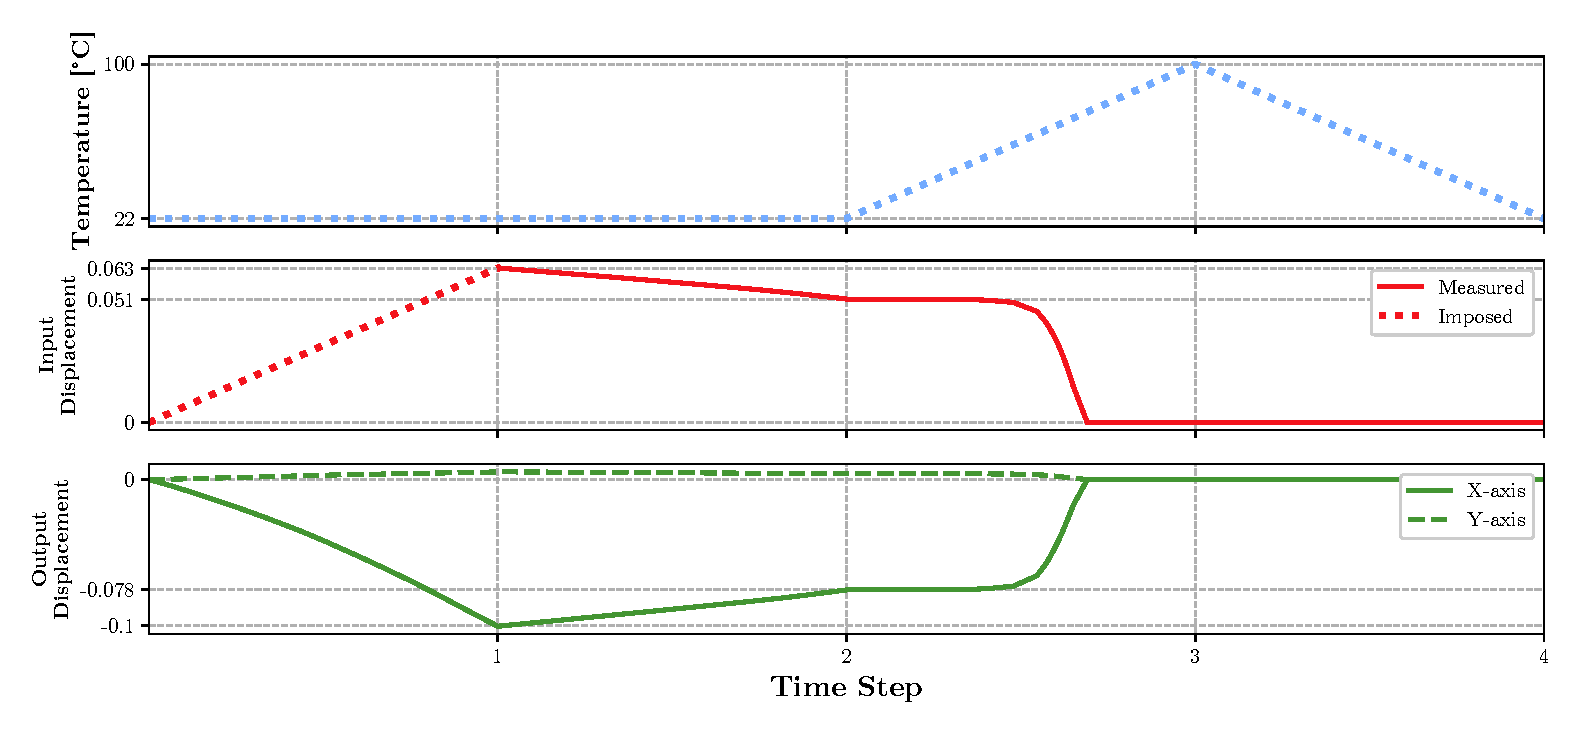
\includegraphics[width=\textwidth]{images/chap5/BM_Inverter30.eps}};
    \begin{scope}[x={(graph.south east)},y={(graph.north west)}]
    % \coordinate (ts0) at (1.54,7.6);
    % \coordinate (ts4) at (17.55,7.6);
    \coordinate (ts0) at (0.085,0.945);
    \coordinate (ts4) at (0.985,0.945);
    \coordinate (ts1) at ($ (ts0)!0.25!(ts4) $);
    \coordinate (ts2) at ($ (ts0)!0.5!(ts4) $);
    \coordinate (ts3) at ($ (ts0)!0.75!(ts4) $);
    \node[anchor=mid,inner sep=0] (ls0) at ($(ts0)!0.5!(ts1) + (0,0.05) $) {\fbox{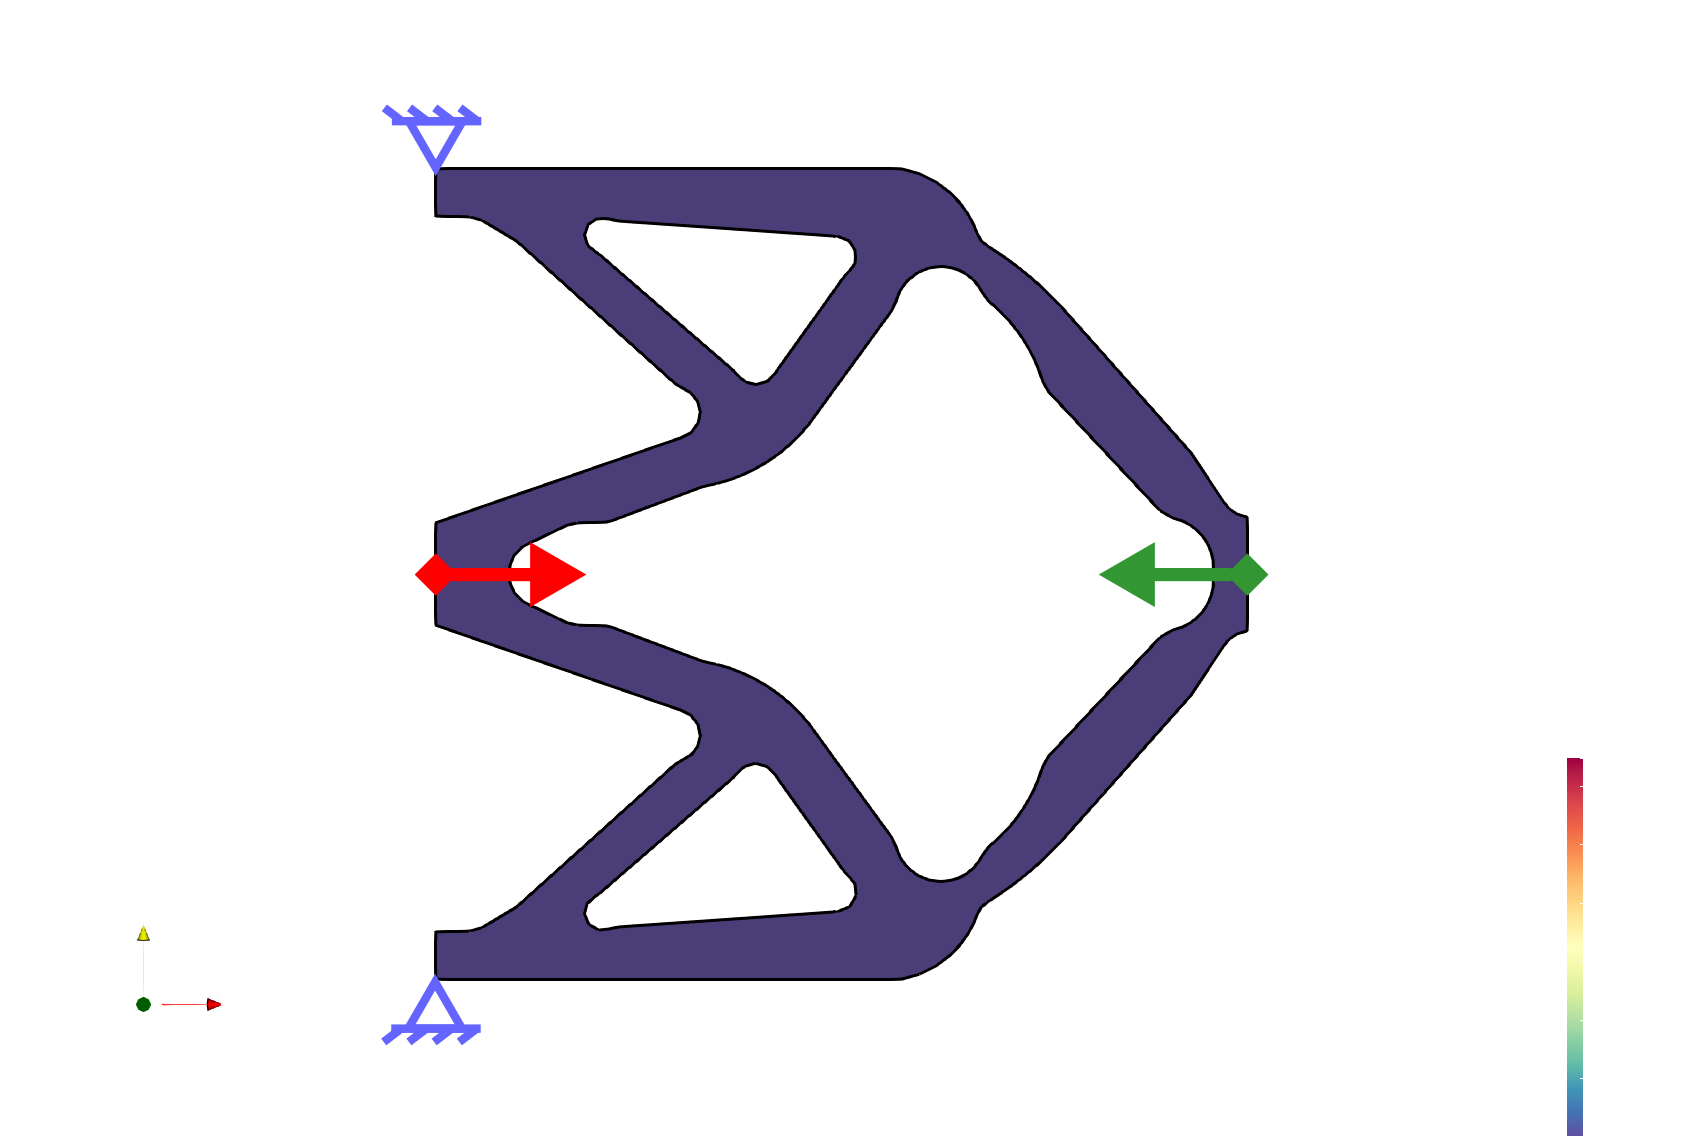
\includegraphics[height = 2cm,trim={11cm 3cm 13cm 3cm},clip]{images/chap5/Inverter_step0_v3.png}}};
    \draw[black, thick, -latex](ls0.west) to [bend right] (ts0);
    \node[anchor=mid,inner sep=0] (ls1) at ($(ts1)!0.5!(ts2) + (0,0.05) $) {\fbox{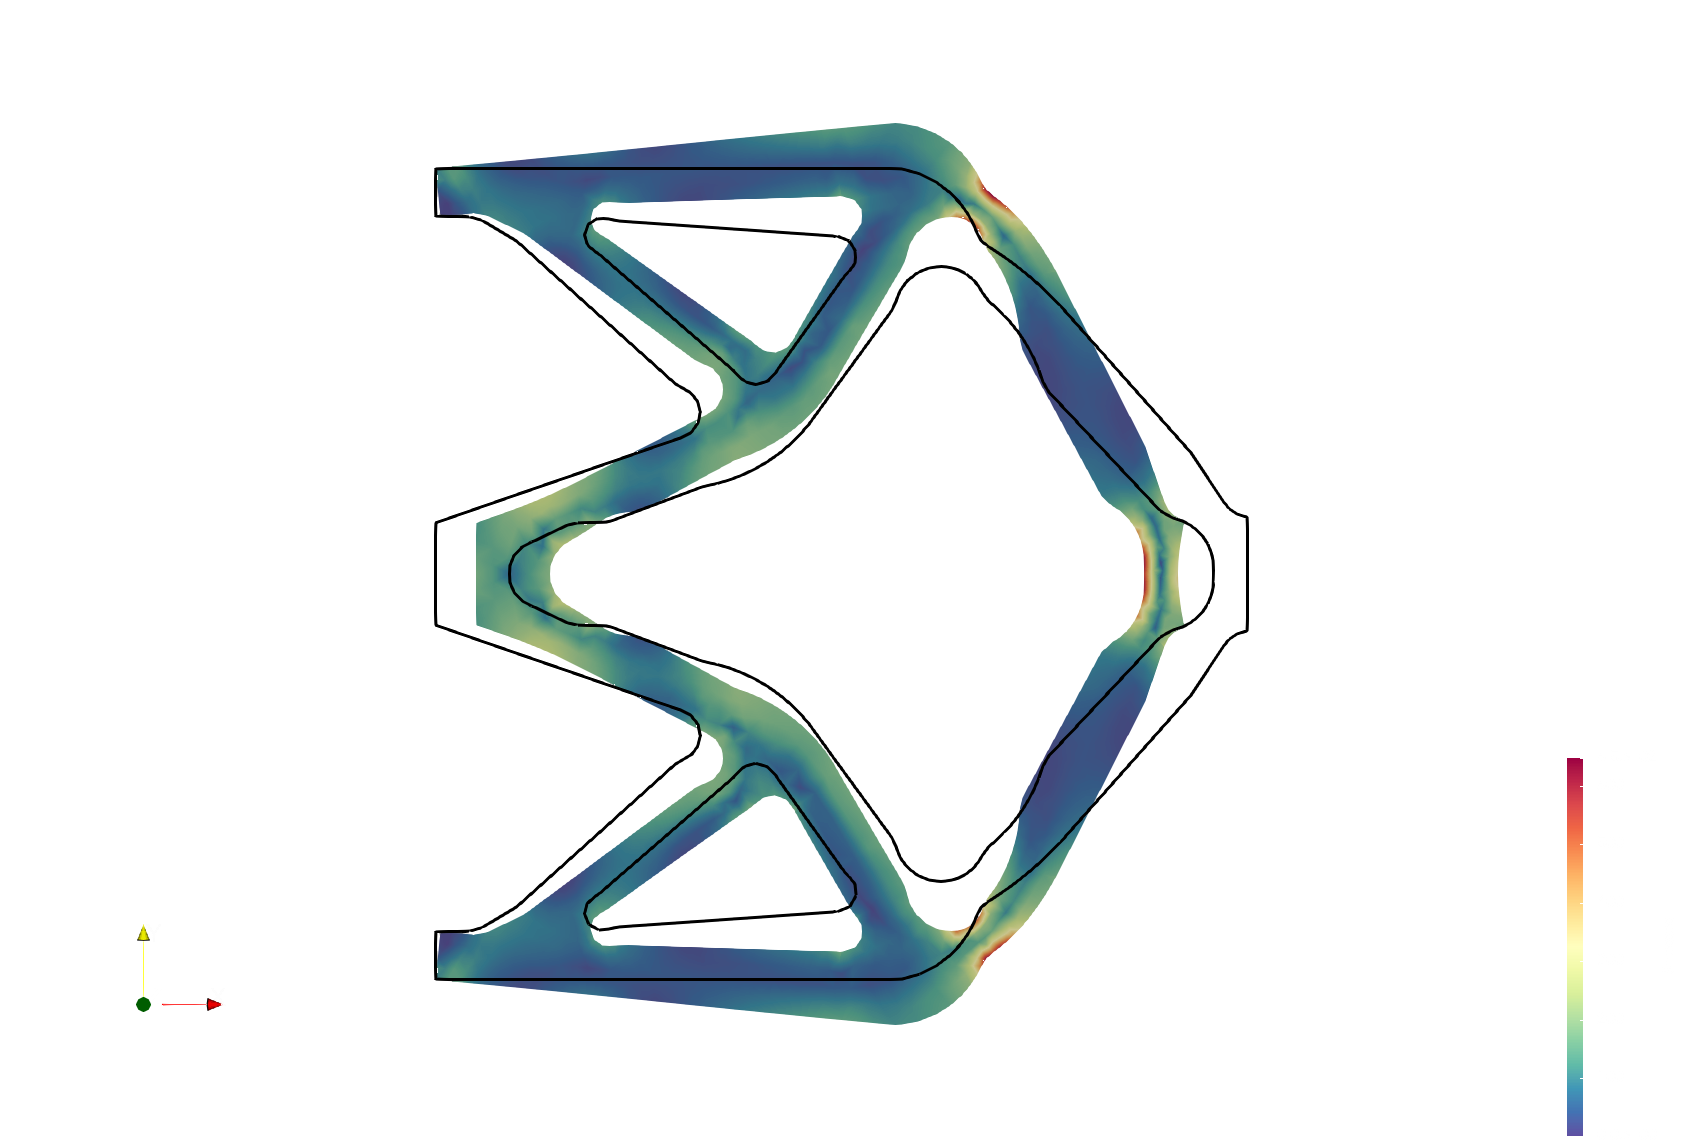
\includegraphics[height = 2cm,trim={11cm 3cm 13cm 3cm},clip]{images/chap5/Inverter_step1.png}}};
    \draw[black, thick, -latex](ls1.west) to [bend right] (ts1);
    \node[anchor=mid,inner sep=0] (ls2) at ($(ts2)!0.5!(ts3) + (0,0.05) $) {\fbox{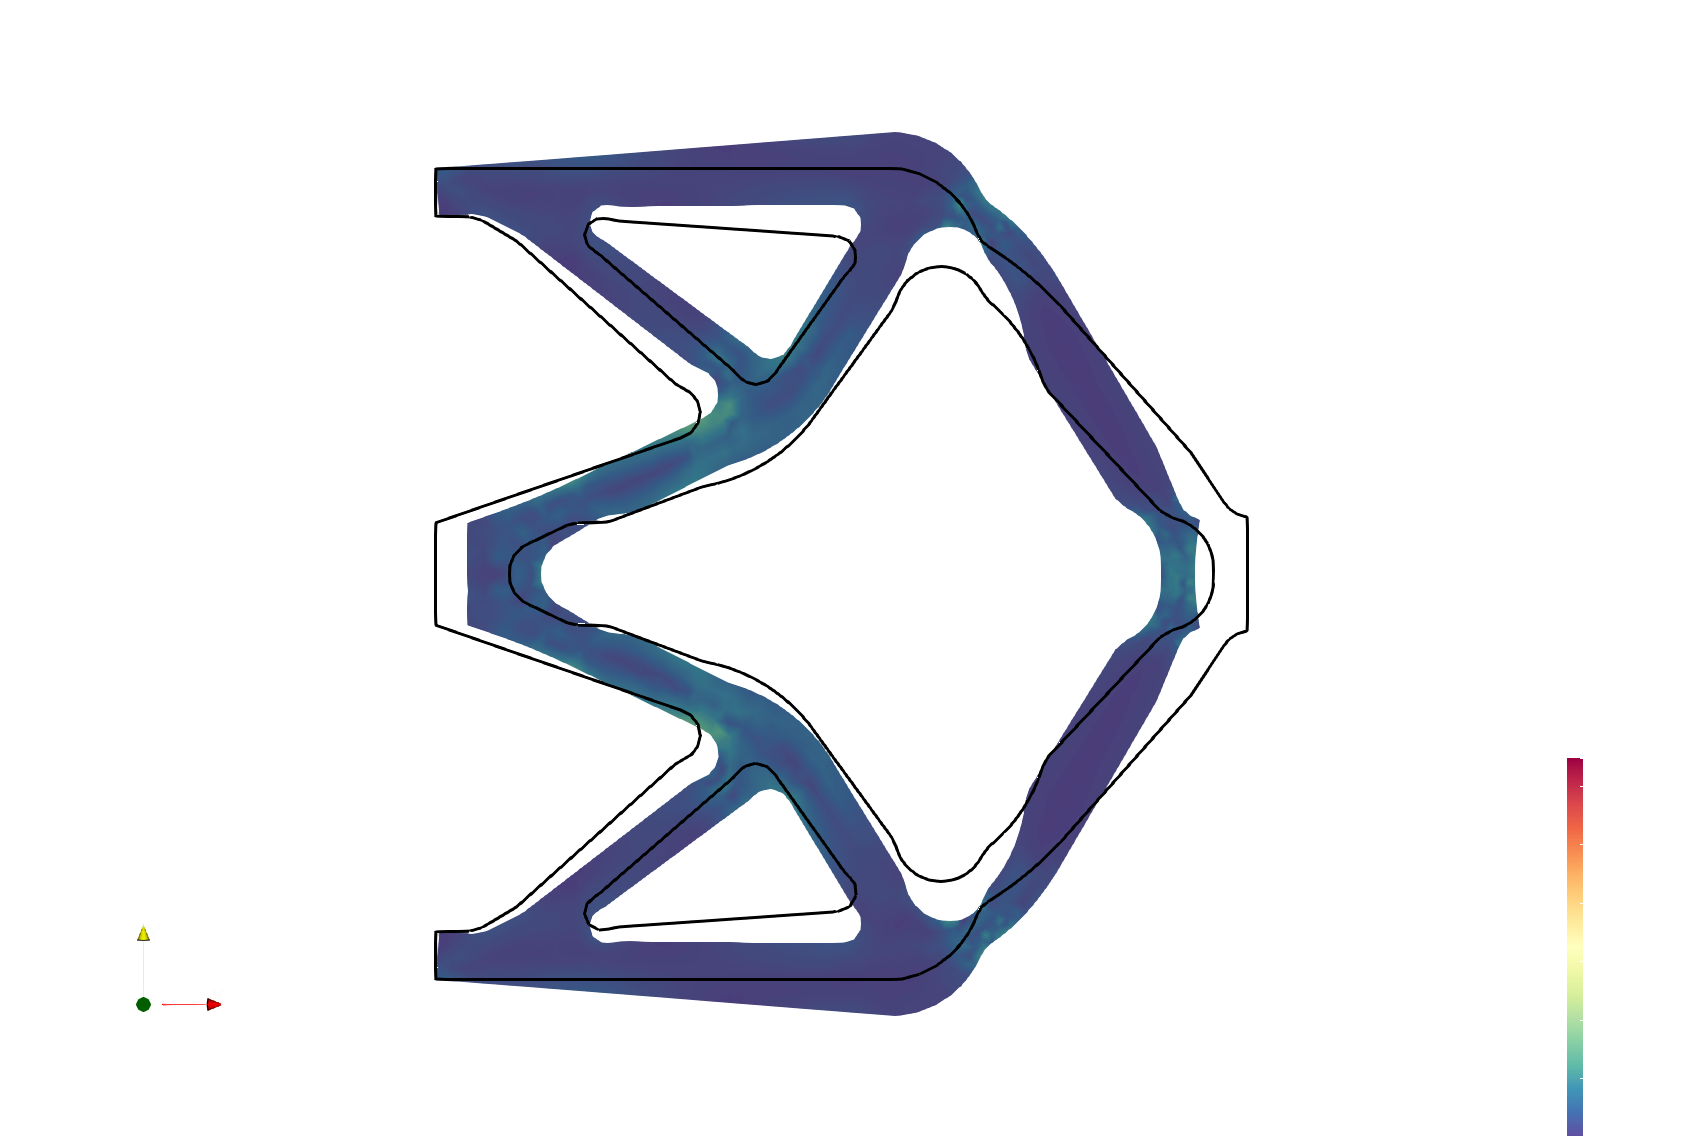
\includegraphics[height = 2cm,trim={11cm 3cm 13cm 3cm},clip]{images/chap5/Inverter_step2.png}}};
    \draw[black, thick, -latex](ls2.west) to [bend right] (ts2);
    \node[anchor=mid,inner sep=0] (ls3) at ($(ts3)!0.5!(ts4) + (0,0.05) $) {\fbox{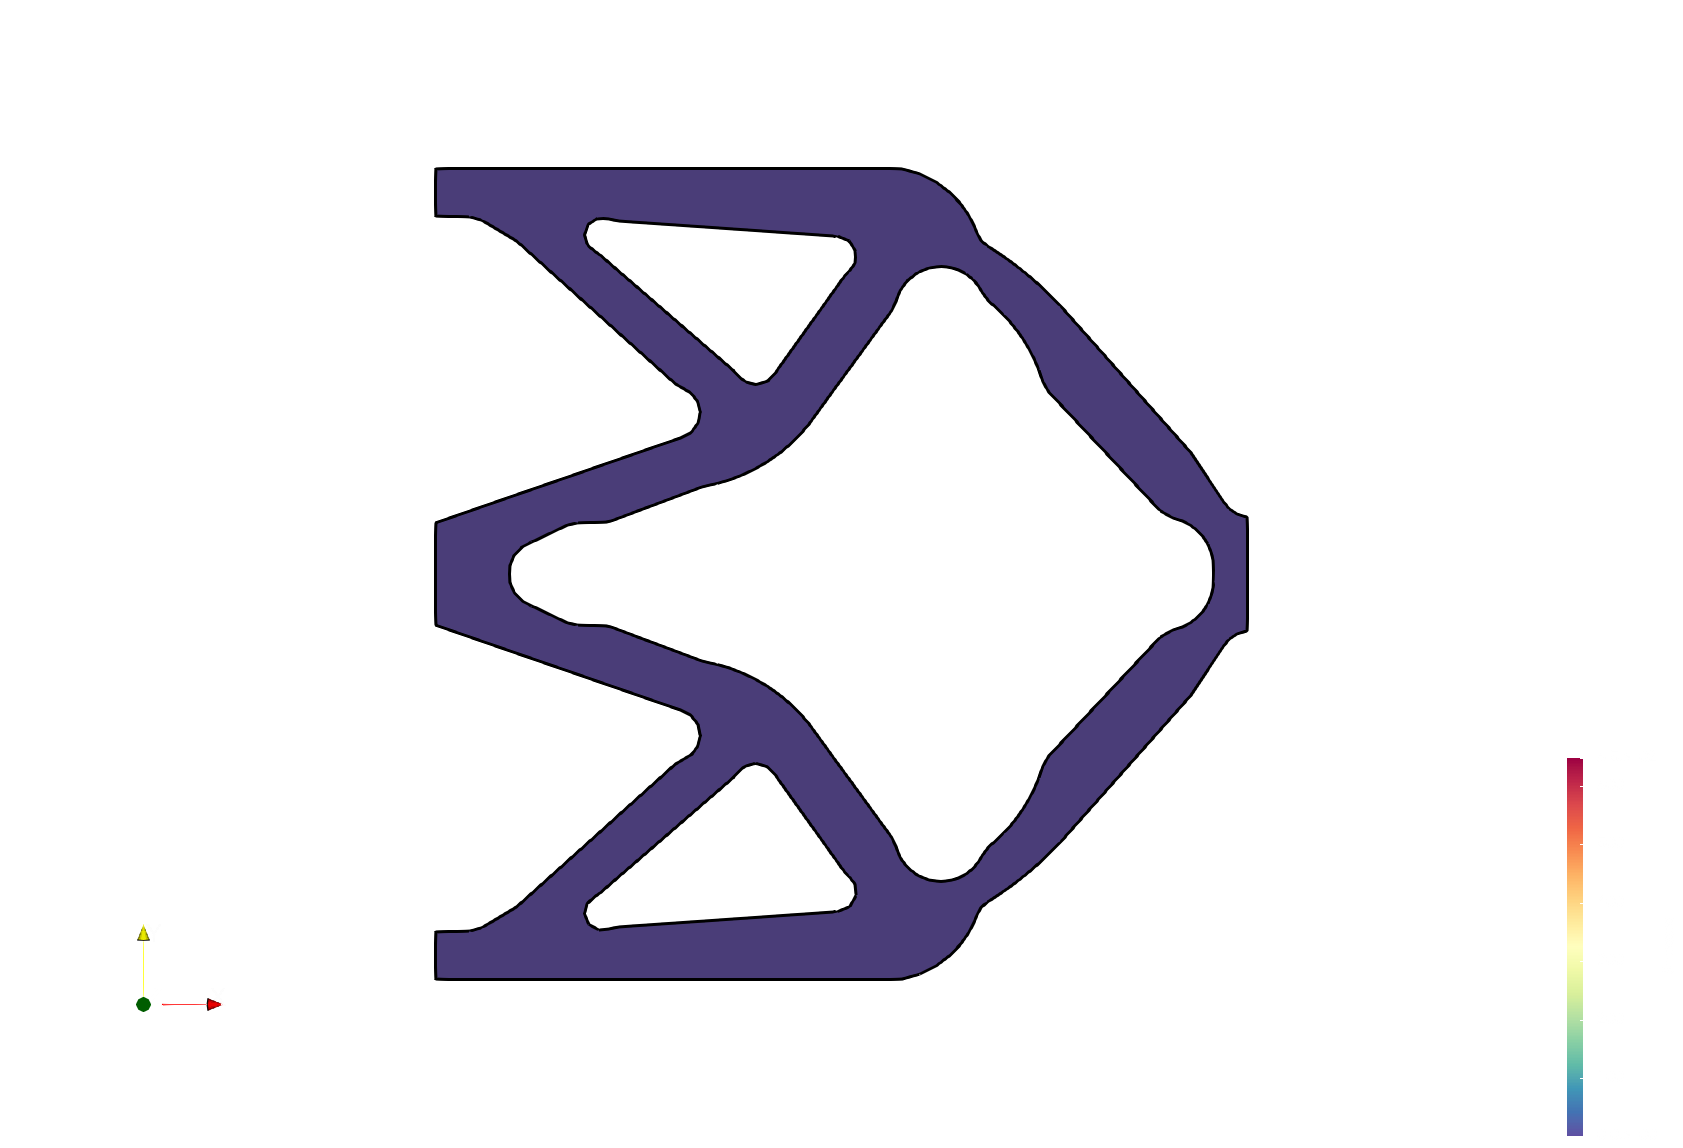
\includegraphics[height = 2cm,trim={11cm 3cm 13cm 3cm},clip]{images/chap5/Inverter_step0.png}}};
    \draw[black, thick, -latex](ls3.west) to [bend right] (ts3);
    \node[anchor=south east,inner sep=0] (ls0) at ($(ts4) + (0,0.015) $) {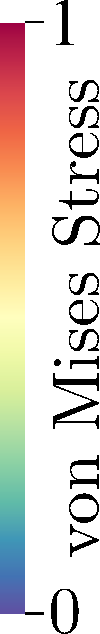
\includegraphics[height = 2.3cm]{images/chap5/Colorbar.pdf}};
    % \draw (0,0) node[circle, fill]{test};
    \filldraw ($ (ts0)!0.25!(ts4) + (0,-0.3)$) circle (1.5pt) node[anchor=north west] {$\epsilon_\text{loaded}$};
    \filldraw ($ (ts0)!0.5!(ts4) + (0,-0.35)$) circle (1.5pt) node[anchor=south west] {$\epsilon_\text{free}$};
    \filldraw ($ (ts0)!0.25!(ts4) + (0,-0.815)$) circle (1.5pt) node[anchor=south west] {$\varepsilon_\text{loaded}$};
    \filldraw ($ (ts0)!0.5!(ts4) + (0,-0.745)$) circle (1.5pt) node[anchor=south west] {$\varepsilon_\text{free}$};
    \end{scope}
    \end{tikzpicture}%
\end{document}

    \caption{Results of the shape memory effect simulation of the Inverter design. Here, the displacements are calculated relatively to the design domain size $L$. The displacements observed between time steps 1 and 2 show a strain retention of $\alpha_\epsilon$ = 77.6\% confirming the presence of the shape memory effect.}
    \label{fig:InverterAnsysSimu}
\end{figure}

\begin{figure}[hbt!]
    \centering
    % !TEX root = ../sethomas_thesis_main.tex
\documentclass[border=1mm,
               class=article
               preview]{standalone}
\usepackage{tikz}
\begin{document}
\begin{tikzpicture}
    \node[anchor=south west,inner sep=0] (graph) at (0,0) {\resizebox{\columnwidth}{!}{%% Creator: Matplotlib, PGF backend
%%
%% To include the figure in your LaTeX document, write
%%   \input{<filename>.pgf}
%%
%% Make sure the required packages are loaded in your preamble
%%   \usepackage{pgf}
%%
%% and, on pdftex
%%   \usepackage[utf8]{inputenc}\DeclareUnicodeCharacter{2212}{-}
%%
%% or, on luatex and xetex
%%   \usepackage{unicode-math}
%%
%% Figures using additional raster images can only be included by \input if
%% they are in the same directory as the main LaTeX file. For loading figures
%% from other directories you can use the `import` package
%%   \usepackage{import}
%%
%% and then include the figures with
%%   \import{<path to file>}{<filename>.pgf}
%%
%% Matplotlib used the following preamble
%%
\begingroup%
\makeatletter%
\begin{pgfpicture}%
\pgfpathrectangle{\pgfpointorigin}{\pgfqpoint{8.648303in}{4.649344in}}%
\pgfusepath{use as bounding box, clip}%
\begin{pgfscope}%
\pgfsetbuttcap%
\pgfsetmiterjoin%
\pgfsetlinewidth{0.000000pt}%
\definecolor{currentstroke}{rgb}{0.000000,0.000000,0.000000}%
\pgfsetstrokecolor{currentstroke}%
\pgfsetstrokeopacity{0.000000}%
\pgfsetdash{}{0pt}%
\pgfpathmoveto{\pgfqpoint{0.000000in}{0.000000in}}%
\pgfpathlineto{\pgfqpoint{8.648303in}{0.000000in}}%
\pgfpathlineto{\pgfqpoint{8.648303in}{4.649344in}}%
\pgfpathlineto{\pgfqpoint{0.000000in}{4.649344in}}%
\pgfpathclose%
\pgfusepath{}%
\end{pgfscope}%
\begin{pgfscope}%
\pgfsetbuttcap%
\pgfsetmiterjoin%
\pgfsetlinewidth{0.000000pt}%
\definecolor{currentstroke}{rgb}{0.000000,0.000000,0.000000}%
\pgfsetstrokecolor{currentstroke}%
\pgfsetstrokeopacity{0.000000}%
\pgfsetdash{}{0pt}%
\pgfpathmoveto{\pgfqpoint{0.763581in}{3.271659in}}%
\pgfpathlineto{\pgfqpoint{8.513581in}{3.271659in}}%
\pgfpathlineto{\pgfqpoint{8.513581in}{4.404012in}}%
\pgfpathlineto{\pgfqpoint{0.763581in}{4.404012in}}%
\pgfpathclose%
\pgfusepath{}%
\end{pgfscope}%
\begin{pgfscope}%
\pgfpathrectangle{\pgfqpoint{0.763581in}{3.271659in}}{\pgfqpoint{7.750000in}{1.132353in}}%
\pgfusepath{clip}%
\pgfsetbuttcap%
\pgfsetroundjoin%
\pgfsetlinewidth{0.803000pt}%
\definecolor{currentstroke}{rgb}{0.690196,0.690196,0.690196}%
\pgfsetstrokecolor{currentstroke}%
\pgfsetdash{{2.960000pt}{1.280000pt}}{0.000000pt}%
\pgfpathmoveto{\pgfqpoint{2.701081in}{3.271659in}}%
\pgfpathlineto{\pgfqpoint{2.701081in}{4.404012in}}%
\pgfusepath{stroke}%
\end{pgfscope}%
\begin{pgfscope}%
\pgfsetbuttcap%
\pgfsetroundjoin%
\definecolor{currentfill}{rgb}{0.000000,0.000000,0.000000}%
\pgfsetfillcolor{currentfill}%
\pgfsetlinewidth{0.803000pt}%
\definecolor{currentstroke}{rgb}{0.000000,0.000000,0.000000}%
\pgfsetstrokecolor{currentstroke}%
\pgfsetdash{}{0pt}%
\pgfsys@defobject{currentmarker}{\pgfqpoint{0.000000in}{-0.048611in}}{\pgfqpoint{0.000000in}{0.000000in}}{%
\pgfpathmoveto{\pgfqpoint{0.000000in}{0.000000in}}%
\pgfpathlineto{\pgfqpoint{0.000000in}{-0.048611in}}%
\pgfusepath{stroke,fill}%
}%
\begin{pgfscope}%
\pgfsys@transformshift{2.701081in}{3.271659in}%
\pgfsys@useobject{currentmarker}{}%
\end{pgfscope}%
\end{pgfscope}%
\begin{pgfscope}%
\pgfpathrectangle{\pgfqpoint{0.763581in}{3.271659in}}{\pgfqpoint{7.750000in}{1.132353in}}%
\pgfusepath{clip}%
\pgfsetbuttcap%
\pgfsetroundjoin%
\pgfsetlinewidth{0.803000pt}%
\definecolor{currentstroke}{rgb}{0.690196,0.690196,0.690196}%
\pgfsetstrokecolor{currentstroke}%
\pgfsetdash{{2.960000pt}{1.280000pt}}{0.000000pt}%
\pgfpathmoveto{\pgfqpoint{4.638581in}{3.271659in}}%
\pgfpathlineto{\pgfqpoint{4.638581in}{4.404012in}}%
\pgfusepath{stroke}%
\end{pgfscope}%
\begin{pgfscope}%
\pgfsetbuttcap%
\pgfsetroundjoin%
\definecolor{currentfill}{rgb}{0.000000,0.000000,0.000000}%
\pgfsetfillcolor{currentfill}%
\pgfsetlinewidth{0.803000pt}%
\definecolor{currentstroke}{rgb}{0.000000,0.000000,0.000000}%
\pgfsetstrokecolor{currentstroke}%
\pgfsetdash{}{0pt}%
\pgfsys@defobject{currentmarker}{\pgfqpoint{0.000000in}{-0.048611in}}{\pgfqpoint{0.000000in}{0.000000in}}{%
\pgfpathmoveto{\pgfqpoint{0.000000in}{0.000000in}}%
\pgfpathlineto{\pgfqpoint{0.000000in}{-0.048611in}}%
\pgfusepath{stroke,fill}%
}%
\begin{pgfscope}%
\pgfsys@transformshift{4.638581in}{3.271659in}%
\pgfsys@useobject{currentmarker}{}%
\end{pgfscope}%
\end{pgfscope}%
\begin{pgfscope}%
\pgfpathrectangle{\pgfqpoint{0.763581in}{3.271659in}}{\pgfqpoint{7.750000in}{1.132353in}}%
\pgfusepath{clip}%
\pgfsetbuttcap%
\pgfsetroundjoin%
\pgfsetlinewidth{0.803000pt}%
\definecolor{currentstroke}{rgb}{0.690196,0.690196,0.690196}%
\pgfsetstrokecolor{currentstroke}%
\pgfsetdash{{2.960000pt}{1.280000pt}}{0.000000pt}%
\pgfpathmoveto{\pgfqpoint{6.576081in}{3.271659in}}%
\pgfpathlineto{\pgfqpoint{6.576081in}{4.404012in}}%
\pgfusepath{stroke}%
\end{pgfscope}%
\begin{pgfscope}%
\pgfsetbuttcap%
\pgfsetroundjoin%
\definecolor{currentfill}{rgb}{0.000000,0.000000,0.000000}%
\pgfsetfillcolor{currentfill}%
\pgfsetlinewidth{0.803000pt}%
\definecolor{currentstroke}{rgb}{0.000000,0.000000,0.000000}%
\pgfsetstrokecolor{currentstroke}%
\pgfsetdash{}{0pt}%
\pgfsys@defobject{currentmarker}{\pgfqpoint{0.000000in}{-0.048611in}}{\pgfqpoint{0.000000in}{0.000000in}}{%
\pgfpathmoveto{\pgfqpoint{0.000000in}{0.000000in}}%
\pgfpathlineto{\pgfqpoint{0.000000in}{-0.048611in}}%
\pgfusepath{stroke,fill}%
}%
\begin{pgfscope}%
\pgfsys@transformshift{6.576081in}{3.271659in}%
\pgfsys@useobject{currentmarker}{}%
\end{pgfscope}%
\end{pgfscope}%
\begin{pgfscope}%
\pgfpathrectangle{\pgfqpoint{0.763581in}{3.271659in}}{\pgfqpoint{7.750000in}{1.132353in}}%
\pgfusepath{clip}%
\pgfsetbuttcap%
\pgfsetroundjoin%
\pgfsetlinewidth{0.803000pt}%
\definecolor{currentstroke}{rgb}{0.690196,0.690196,0.690196}%
\pgfsetstrokecolor{currentstroke}%
\pgfsetdash{{2.960000pt}{1.280000pt}}{0.000000pt}%
\pgfpathmoveto{\pgfqpoint{8.513581in}{3.271659in}}%
\pgfpathlineto{\pgfqpoint{8.513581in}{4.404012in}}%
\pgfusepath{stroke}%
\end{pgfscope}%
\begin{pgfscope}%
\pgfsetbuttcap%
\pgfsetroundjoin%
\definecolor{currentfill}{rgb}{0.000000,0.000000,0.000000}%
\pgfsetfillcolor{currentfill}%
\pgfsetlinewidth{0.803000pt}%
\definecolor{currentstroke}{rgb}{0.000000,0.000000,0.000000}%
\pgfsetstrokecolor{currentstroke}%
\pgfsetdash{}{0pt}%
\pgfsys@defobject{currentmarker}{\pgfqpoint{0.000000in}{-0.048611in}}{\pgfqpoint{0.000000in}{0.000000in}}{%
\pgfpathmoveto{\pgfqpoint{0.000000in}{0.000000in}}%
\pgfpathlineto{\pgfqpoint{0.000000in}{-0.048611in}}%
\pgfusepath{stroke,fill}%
}%
\begin{pgfscope}%
\pgfsys@transformshift{8.513581in}{3.271659in}%
\pgfsys@useobject{currentmarker}{}%
\end{pgfscope}%
\end{pgfscope}%
\begin{pgfscope}%
\pgfpathrectangle{\pgfqpoint{0.763581in}{3.271659in}}{\pgfqpoint{7.750000in}{1.132353in}}%
\pgfusepath{clip}%
\pgfsetbuttcap%
\pgfsetroundjoin%
\pgfsetlinewidth{0.803000pt}%
\definecolor{currentstroke}{rgb}{0.690196,0.690196,0.690196}%
\pgfsetstrokecolor{currentstroke}%
\pgfsetdash{{2.960000pt}{1.280000pt}}{0.000000pt}%
\pgfpathmoveto{\pgfqpoint{0.763581in}{3.323129in}}%
\pgfpathlineto{\pgfqpoint{8.513581in}{3.323129in}}%
\pgfusepath{stroke}%
\end{pgfscope}%
\begin{pgfscope}%
\pgfsetbuttcap%
\pgfsetroundjoin%
\definecolor{currentfill}{rgb}{0.000000,0.000000,0.000000}%
\pgfsetfillcolor{currentfill}%
\pgfsetlinewidth{0.803000pt}%
\definecolor{currentstroke}{rgb}{0.000000,0.000000,0.000000}%
\pgfsetstrokecolor{currentstroke}%
\pgfsetdash{}{0pt}%
\pgfsys@defobject{currentmarker}{\pgfqpoint{-0.048611in}{0.000000in}}{\pgfqpoint{-0.000000in}{0.000000in}}{%
\pgfpathmoveto{\pgfqpoint{-0.000000in}{0.000000in}}%
\pgfpathlineto{\pgfqpoint{-0.048611in}{0.000000in}}%
\pgfusepath{stroke,fill}%
}%
\begin{pgfscope}%
\pgfsys@transformshift{0.763581in}{3.323129in}%
\pgfsys@useobject{currentmarker}{}%
\end{pgfscope}%
\end{pgfscope}%
\begin{pgfscope}%
\definecolor{textcolor}{rgb}{0.000000,0.000000,0.000000}%
\pgfsetstrokecolor{textcolor}%
\pgfsetfillcolor{textcolor}%
\pgftext[x=0.527469in, y=3.274904in, left, base]{\color{textcolor}\rmfamily\fontsize{10.000000}{12.000000}\selectfont \(\displaystyle {22}\)}%
\end{pgfscope}%
\begin{pgfscope}%
\pgfpathrectangle{\pgfqpoint{0.763581in}{3.271659in}}{\pgfqpoint{7.750000in}{1.132353in}}%
\pgfusepath{clip}%
\pgfsetbuttcap%
\pgfsetroundjoin%
\pgfsetlinewidth{0.803000pt}%
\definecolor{currentstroke}{rgb}{0.690196,0.690196,0.690196}%
\pgfsetstrokecolor{currentstroke}%
\pgfsetdash{{2.960000pt}{1.280000pt}}{0.000000pt}%
\pgfpathmoveto{\pgfqpoint{0.763581in}{4.352541in}}%
\pgfpathlineto{\pgfqpoint{8.513581in}{4.352541in}}%
\pgfusepath{stroke}%
\end{pgfscope}%
\begin{pgfscope}%
\pgfsetbuttcap%
\pgfsetroundjoin%
\definecolor{currentfill}{rgb}{0.000000,0.000000,0.000000}%
\pgfsetfillcolor{currentfill}%
\pgfsetlinewidth{0.803000pt}%
\definecolor{currentstroke}{rgb}{0.000000,0.000000,0.000000}%
\pgfsetstrokecolor{currentstroke}%
\pgfsetdash{}{0pt}%
\pgfsys@defobject{currentmarker}{\pgfqpoint{-0.048611in}{0.000000in}}{\pgfqpoint{-0.000000in}{0.000000in}}{%
\pgfpathmoveto{\pgfqpoint{-0.000000in}{0.000000in}}%
\pgfpathlineto{\pgfqpoint{-0.048611in}{0.000000in}}%
\pgfusepath{stroke,fill}%
}%
\begin{pgfscope}%
\pgfsys@transformshift{0.763581in}{4.352541in}%
\pgfsys@useobject{currentmarker}{}%
\end{pgfscope}%
\end{pgfscope}%
\begin{pgfscope}%
\definecolor{textcolor}{rgb}{0.000000,0.000000,0.000000}%
\pgfsetstrokecolor{textcolor}%
\pgfsetfillcolor{textcolor}%
\pgftext[x=0.458024in, y=4.304316in, left, base]{\color{textcolor}\rmfamily\fontsize{10.000000}{12.000000}\selectfont \(\displaystyle {160}\)}%
\end{pgfscope}%
\begin{pgfscope}%
\definecolor{textcolor}{rgb}{0.000000,0.000000,0.000000}%
\pgfsetstrokecolor{textcolor}%
\pgfsetfillcolor{textcolor}%
\pgftext[x=0.402469in,y=3.837835in,,bottom,rotate=90.000000]{\color{textcolor}\rmfamily\fontsize{12.000000}{14.400000}\bfseries\selectfont Temperature [°C]}%
\end{pgfscope}%
\begin{pgfscope}%
\pgfpathrectangle{\pgfqpoint{0.763581in}{3.271659in}}{\pgfqpoint{7.750000in}{1.132353in}}%
\pgfusepath{clip}%
\pgfsetbuttcap%
\pgfsetroundjoin%
\pgfsetlinewidth{3.011250pt}%
\definecolor{currentstroke}{rgb}{0.450980,0.670588,1.000000}%
\pgfsetstrokecolor{currentstroke}%
\pgfsetdash{{3.000000pt}{4.950000pt}}{0.000000pt}%
\pgfpathmoveto{\pgfqpoint{0.763581in}{3.323129in}}%
\pgfpathlineto{\pgfqpoint{0.776497in}{3.323129in}}%
\pgfpathlineto{\pgfqpoint{0.789413in}{3.323129in}}%
\pgfpathlineto{\pgfqpoint{0.808788in}{3.323129in}}%
\pgfpathlineto{\pgfqpoint{0.837851in}{3.323129in}}%
\pgfpathlineto{\pgfqpoint{0.881444in}{3.323129in}}%
\pgfpathlineto{\pgfqpoint{0.925038in}{3.323129in}}%
\pgfpathlineto{\pgfqpoint{0.990423in}{3.323129in}}%
\pgfpathlineto{\pgfqpoint{1.055814in}{3.323129in}}%
\pgfpathlineto{\pgfqpoint{1.121204in}{3.323129in}}%
\pgfpathlineto{\pgfqpoint{1.170262in}{3.323129in}}%
\pgfpathlineto{\pgfqpoint{1.207036in}{3.323129in}}%
\pgfpathlineto{\pgfqpoint{1.243809in}{3.323129in}}%
\pgfpathlineto{\pgfqpoint{1.298989in}{3.323129in}}%
\pgfpathlineto{\pgfqpoint{1.381759in}{3.323129in}}%
\pgfpathlineto{\pgfqpoint{1.464510in}{3.323129in}}%
\pgfpathlineto{\pgfqpoint{1.588646in}{3.323129in}}%
\pgfpathlineto{\pgfqpoint{1.712801in}{3.323129in}}%
\pgfpathlineto{\pgfqpoint{1.836936in}{3.323129in}}%
\pgfpathlineto{\pgfqpoint{1.961072in}{3.323129in}}%
\pgfpathlineto{\pgfqpoint{2.090245in}{3.323129in}}%
\pgfpathlineto{\pgfqpoint{2.219399in}{3.323129in}}%
\pgfpathlineto{\pgfqpoint{2.348572in}{3.323129in}}%
\pgfpathlineto{\pgfqpoint{2.477745in}{3.323129in}}%
\pgfpathlineto{\pgfqpoint{2.574620in}{3.323129in}}%
\pgfpathlineto{\pgfqpoint{2.647276in}{3.323129in}}%
\pgfpathlineto{\pgfqpoint{2.701081in}{3.323129in}}%
\pgfpathlineto{\pgfqpoint{2.714062in}{3.323129in}}%
\pgfpathlineto{\pgfqpoint{2.726849in}{3.323129in}}%
\pgfpathlineto{\pgfqpoint{2.746224in}{3.323129in}}%
\pgfpathlineto{\pgfqpoint{2.775287in}{3.323129in}}%
\pgfpathlineto{\pgfqpoint{2.818881in}{3.323129in}}%
\pgfpathlineto{\pgfqpoint{2.884368in}{3.323129in}}%
\pgfpathlineto{\pgfqpoint{2.982406in}{3.323129in}}%
\pgfpathlineto{\pgfqpoint{3.111637in}{3.323129in}}%
\pgfpathlineto{\pgfqpoint{3.240674in}{3.323129in}}%
\pgfpathlineto{\pgfqpoint{3.369906in}{3.323129in}}%
\pgfpathlineto{\pgfqpoint{3.499137in}{3.323129in}}%
\pgfpathlineto{\pgfqpoint{3.628174in}{3.323129in}}%
\pgfpathlineto{\pgfqpoint{3.757406in}{3.323129in}}%
\pgfpathlineto{\pgfqpoint{3.886637in}{3.323129in}}%
\pgfpathlineto{\pgfqpoint{4.015674in}{3.323129in}}%
\pgfpathlineto{\pgfqpoint{4.144906in}{3.323129in}}%
\pgfpathlineto{\pgfqpoint{4.274137in}{3.323129in}}%
\pgfpathlineto{\pgfqpoint{4.403174in}{3.323129in}}%
\pgfpathlineto{\pgfqpoint{4.532406in}{3.323129in}}%
\pgfpathlineto{\pgfqpoint{4.638581in}{3.323129in}}%
\pgfpathlineto{\pgfqpoint{4.651562in}{3.330029in}}%
\pgfpathlineto{\pgfqpoint{4.664349in}{3.336818in}}%
\pgfpathlineto{\pgfqpoint{4.683724in}{3.347112in}}%
\pgfpathlineto{\pgfqpoint{4.712787in}{3.362553in}}%
\pgfpathlineto{\pgfqpoint{4.756381in}{3.385715in}}%
\pgfpathlineto{\pgfqpoint{4.821868in}{3.420513in}}%
\pgfpathlineto{\pgfqpoint{4.919906in}{3.472603in}}%
\pgfpathlineto{\pgfqpoint{5.049137in}{3.541260in}}%
\pgfpathlineto{\pgfqpoint{5.178174in}{3.609821in}}%
\pgfpathlineto{\pgfqpoint{5.307406in}{3.678485in}}%
\pgfpathlineto{\pgfqpoint{5.436637in}{3.747143in}}%
\pgfpathlineto{\pgfqpoint{5.565674in}{3.815703in}}%
\pgfpathlineto{\pgfqpoint{5.630387in}{3.850084in}}%
\pgfpathlineto{\pgfqpoint{5.678824in}{3.875819in}}%
\pgfpathlineto{\pgfqpoint{5.697037in}{3.885494in}}%
\pgfpathlineto{\pgfqpoint{5.710599in}{3.892700in}}%
\pgfpathlineto{\pgfqpoint{5.720868in}{3.898160in}}%
\pgfpathlineto{\pgfqpoint{5.728424in}{3.902174in}}%
\pgfpathlineto{\pgfqpoint{5.736174in}{3.906314in}}%
\pgfpathlineto{\pgfqpoint{5.747606in}{3.912356in}}%
\pgfpathlineto{\pgfqpoint{5.750512in}{3.913922in}}%
\pgfpathlineto{\pgfqpoint{5.751481in}{3.914444in}}%
\pgfpathlineto{\pgfqpoint{5.752449in}{3.914967in}}%
\pgfpathlineto{\pgfqpoint{5.753031in}{3.915265in}}%
\pgfpathlineto{\pgfqpoint{5.753612in}{3.915563in}}%
\pgfpathlineto{\pgfqpoint{5.754387in}{3.915936in}}%
\pgfpathlineto{\pgfqpoint{5.755937in}{3.916757in}}%
\pgfpathlineto{\pgfqpoint{5.757293in}{3.917503in}}%
\pgfpathlineto{\pgfqpoint{5.758262in}{3.918025in}}%
\pgfpathlineto{\pgfqpoint{5.759231in}{3.918547in}}%
\pgfpathlineto{\pgfqpoint{5.760781in}{3.919368in}}%
\pgfpathlineto{\pgfqpoint{5.763106in}{3.920636in}}%
\pgfpathlineto{\pgfqpoint{5.765431in}{3.921829in}}%
\pgfpathlineto{\pgfqpoint{5.767756in}{3.923097in}}%
\pgfpathlineto{\pgfqpoint{5.771049in}{3.924813in}}%
\pgfpathlineto{\pgfqpoint{5.773762in}{3.926230in}}%
\pgfpathlineto{\pgfqpoint{5.775699in}{3.927275in}}%
\pgfpathlineto{\pgfqpoint{5.777637in}{3.928319in}}%
\pgfpathlineto{\pgfqpoint{5.780543in}{3.929886in}}%
\pgfpathlineto{\pgfqpoint{5.783449in}{3.931378in}}%
\pgfpathlineto{\pgfqpoint{5.785581in}{3.932571in}}%
\pgfpathlineto{\pgfqpoint{5.787324in}{3.933466in}}%
\pgfpathlineto{\pgfqpoint{5.788874in}{3.934287in}}%
\pgfpathlineto{\pgfqpoint{5.791393in}{3.935629in}}%
\pgfpathlineto{\pgfqpoint{5.793912in}{3.936972in}}%
\pgfpathlineto{\pgfqpoint{5.796237in}{3.938240in}}%
\pgfpathlineto{\pgfqpoint{5.798174in}{3.939210in}}%
\pgfpathlineto{\pgfqpoint{5.799918in}{3.940180in}}%
\pgfpathlineto{\pgfqpoint{5.801274in}{3.940851in}}%
\pgfpathlineto{\pgfqpoint{5.802437in}{3.941522in}}%
\pgfpathlineto{\pgfqpoint{5.803212in}{3.941895in}}%
\pgfpathlineto{\pgfqpoint{5.803793in}{3.942194in}}%
\pgfpathlineto{\pgfqpoint{6.576081in}{4.352541in}}%
\pgfpathlineto{\pgfqpoint{8.513581in}{3.323129in}}%
\pgfusepath{stroke}%
\end{pgfscope}%
\begin{pgfscope}%
\pgfsetrectcap%
\pgfsetmiterjoin%
\pgfsetlinewidth{0.803000pt}%
\definecolor{currentstroke}{rgb}{0.000000,0.000000,0.000000}%
\pgfsetstrokecolor{currentstroke}%
\pgfsetdash{}{0pt}%
\pgfpathmoveto{\pgfqpoint{0.763581in}{3.271659in}}%
\pgfpathlineto{\pgfqpoint{0.763581in}{4.404012in}}%
\pgfusepath{stroke}%
\end{pgfscope}%
\begin{pgfscope}%
\pgfsetrectcap%
\pgfsetmiterjoin%
\pgfsetlinewidth{0.803000pt}%
\definecolor{currentstroke}{rgb}{0.000000,0.000000,0.000000}%
\pgfsetstrokecolor{currentstroke}%
\pgfsetdash{}{0pt}%
\pgfpathmoveto{\pgfqpoint{8.513581in}{3.271659in}}%
\pgfpathlineto{\pgfqpoint{8.513581in}{4.404012in}}%
\pgfusepath{stroke}%
\end{pgfscope}%
\begin{pgfscope}%
\pgfsetrectcap%
\pgfsetmiterjoin%
\pgfsetlinewidth{0.803000pt}%
\definecolor{currentstroke}{rgb}{0.000000,0.000000,0.000000}%
\pgfsetstrokecolor{currentstroke}%
\pgfsetdash{}{0pt}%
\pgfpathmoveto{\pgfqpoint{0.763581in}{3.271659in}}%
\pgfpathlineto{\pgfqpoint{8.513581in}{3.271659in}}%
\pgfusepath{stroke}%
\end{pgfscope}%
\begin{pgfscope}%
\pgfsetrectcap%
\pgfsetmiterjoin%
\pgfsetlinewidth{0.803000pt}%
\definecolor{currentstroke}{rgb}{0.000000,0.000000,0.000000}%
\pgfsetstrokecolor{currentstroke}%
\pgfsetdash{}{0pt}%
\pgfpathmoveto{\pgfqpoint{0.763581in}{4.404012in}}%
\pgfpathlineto{\pgfqpoint{8.513581in}{4.404012in}}%
\pgfusepath{stroke}%
\end{pgfscope}%
\begin{pgfscope}%
\pgfsetbuttcap%
\pgfsetmiterjoin%
\pgfsetlinewidth{0.000000pt}%
\definecolor{currentstroke}{rgb}{0.000000,0.000000,0.000000}%
\pgfsetstrokecolor{currentstroke}%
\pgfsetstrokeopacity{0.000000}%
\pgfsetdash{}{0pt}%
\pgfpathmoveto{\pgfqpoint{0.763581in}{1.912835in}}%
\pgfpathlineto{\pgfqpoint{8.513581in}{1.912835in}}%
\pgfpathlineto{\pgfqpoint{8.513581in}{3.045188in}}%
\pgfpathlineto{\pgfqpoint{0.763581in}{3.045188in}}%
\pgfpathclose%
\pgfusepath{}%
\end{pgfscope}%
\begin{pgfscope}%
\pgfpathrectangle{\pgfqpoint{0.763581in}{1.912835in}}{\pgfqpoint{7.750000in}{1.132353in}}%
\pgfusepath{clip}%
\pgfsetbuttcap%
\pgfsetroundjoin%
\pgfsetlinewidth{0.803000pt}%
\definecolor{currentstroke}{rgb}{0.690196,0.690196,0.690196}%
\pgfsetstrokecolor{currentstroke}%
\pgfsetdash{{2.960000pt}{1.280000pt}}{0.000000pt}%
\pgfpathmoveto{\pgfqpoint{2.701081in}{1.912835in}}%
\pgfpathlineto{\pgfqpoint{2.701081in}{3.045188in}}%
\pgfusepath{stroke}%
\end{pgfscope}%
\begin{pgfscope}%
\pgfsetbuttcap%
\pgfsetroundjoin%
\definecolor{currentfill}{rgb}{0.000000,0.000000,0.000000}%
\pgfsetfillcolor{currentfill}%
\pgfsetlinewidth{0.803000pt}%
\definecolor{currentstroke}{rgb}{0.000000,0.000000,0.000000}%
\pgfsetstrokecolor{currentstroke}%
\pgfsetdash{}{0pt}%
\pgfsys@defobject{currentmarker}{\pgfqpoint{0.000000in}{-0.048611in}}{\pgfqpoint{0.000000in}{0.000000in}}{%
\pgfpathmoveto{\pgfqpoint{0.000000in}{0.000000in}}%
\pgfpathlineto{\pgfqpoint{0.000000in}{-0.048611in}}%
\pgfusepath{stroke,fill}%
}%
\begin{pgfscope}%
\pgfsys@transformshift{2.701081in}{1.912835in}%
\pgfsys@useobject{currentmarker}{}%
\end{pgfscope}%
\end{pgfscope}%
\begin{pgfscope}%
\pgfpathrectangle{\pgfqpoint{0.763581in}{1.912835in}}{\pgfqpoint{7.750000in}{1.132353in}}%
\pgfusepath{clip}%
\pgfsetbuttcap%
\pgfsetroundjoin%
\pgfsetlinewidth{0.803000pt}%
\definecolor{currentstroke}{rgb}{0.690196,0.690196,0.690196}%
\pgfsetstrokecolor{currentstroke}%
\pgfsetdash{{2.960000pt}{1.280000pt}}{0.000000pt}%
\pgfpathmoveto{\pgfqpoint{4.638581in}{1.912835in}}%
\pgfpathlineto{\pgfqpoint{4.638581in}{3.045188in}}%
\pgfusepath{stroke}%
\end{pgfscope}%
\begin{pgfscope}%
\pgfsetbuttcap%
\pgfsetroundjoin%
\definecolor{currentfill}{rgb}{0.000000,0.000000,0.000000}%
\pgfsetfillcolor{currentfill}%
\pgfsetlinewidth{0.803000pt}%
\definecolor{currentstroke}{rgb}{0.000000,0.000000,0.000000}%
\pgfsetstrokecolor{currentstroke}%
\pgfsetdash{}{0pt}%
\pgfsys@defobject{currentmarker}{\pgfqpoint{0.000000in}{-0.048611in}}{\pgfqpoint{0.000000in}{0.000000in}}{%
\pgfpathmoveto{\pgfqpoint{0.000000in}{0.000000in}}%
\pgfpathlineto{\pgfqpoint{0.000000in}{-0.048611in}}%
\pgfusepath{stroke,fill}%
}%
\begin{pgfscope}%
\pgfsys@transformshift{4.638581in}{1.912835in}%
\pgfsys@useobject{currentmarker}{}%
\end{pgfscope}%
\end{pgfscope}%
\begin{pgfscope}%
\pgfpathrectangle{\pgfqpoint{0.763581in}{1.912835in}}{\pgfqpoint{7.750000in}{1.132353in}}%
\pgfusepath{clip}%
\pgfsetbuttcap%
\pgfsetroundjoin%
\pgfsetlinewidth{0.803000pt}%
\definecolor{currentstroke}{rgb}{0.690196,0.690196,0.690196}%
\pgfsetstrokecolor{currentstroke}%
\pgfsetdash{{2.960000pt}{1.280000pt}}{0.000000pt}%
\pgfpathmoveto{\pgfqpoint{6.576081in}{1.912835in}}%
\pgfpathlineto{\pgfqpoint{6.576081in}{3.045188in}}%
\pgfusepath{stroke}%
\end{pgfscope}%
\begin{pgfscope}%
\pgfsetbuttcap%
\pgfsetroundjoin%
\definecolor{currentfill}{rgb}{0.000000,0.000000,0.000000}%
\pgfsetfillcolor{currentfill}%
\pgfsetlinewidth{0.803000pt}%
\definecolor{currentstroke}{rgb}{0.000000,0.000000,0.000000}%
\pgfsetstrokecolor{currentstroke}%
\pgfsetdash{}{0pt}%
\pgfsys@defobject{currentmarker}{\pgfqpoint{0.000000in}{-0.048611in}}{\pgfqpoint{0.000000in}{0.000000in}}{%
\pgfpathmoveto{\pgfqpoint{0.000000in}{0.000000in}}%
\pgfpathlineto{\pgfqpoint{0.000000in}{-0.048611in}}%
\pgfusepath{stroke,fill}%
}%
\begin{pgfscope}%
\pgfsys@transformshift{6.576081in}{1.912835in}%
\pgfsys@useobject{currentmarker}{}%
\end{pgfscope}%
\end{pgfscope}%
\begin{pgfscope}%
\pgfpathrectangle{\pgfqpoint{0.763581in}{1.912835in}}{\pgfqpoint{7.750000in}{1.132353in}}%
\pgfusepath{clip}%
\pgfsetbuttcap%
\pgfsetroundjoin%
\pgfsetlinewidth{0.803000pt}%
\definecolor{currentstroke}{rgb}{0.690196,0.690196,0.690196}%
\pgfsetstrokecolor{currentstroke}%
\pgfsetdash{{2.960000pt}{1.280000pt}}{0.000000pt}%
\pgfpathmoveto{\pgfqpoint{8.513581in}{1.912835in}}%
\pgfpathlineto{\pgfqpoint{8.513581in}{3.045188in}}%
\pgfusepath{stroke}%
\end{pgfscope}%
\begin{pgfscope}%
\pgfsetbuttcap%
\pgfsetroundjoin%
\definecolor{currentfill}{rgb}{0.000000,0.000000,0.000000}%
\pgfsetfillcolor{currentfill}%
\pgfsetlinewidth{0.803000pt}%
\definecolor{currentstroke}{rgb}{0.000000,0.000000,0.000000}%
\pgfsetstrokecolor{currentstroke}%
\pgfsetdash{}{0pt}%
\pgfsys@defobject{currentmarker}{\pgfqpoint{0.000000in}{-0.048611in}}{\pgfqpoint{0.000000in}{0.000000in}}{%
\pgfpathmoveto{\pgfqpoint{0.000000in}{0.000000in}}%
\pgfpathlineto{\pgfqpoint{0.000000in}{-0.048611in}}%
\pgfusepath{stroke,fill}%
}%
\begin{pgfscope}%
\pgfsys@transformshift{8.513581in}{1.912835in}%
\pgfsys@useobject{currentmarker}{}%
\end{pgfscope}%
\end{pgfscope}%
\begin{pgfscope}%
\pgfpathrectangle{\pgfqpoint{0.763581in}{1.912835in}}{\pgfqpoint{7.750000in}{1.132353in}}%
\pgfusepath{clip}%
\pgfsetbuttcap%
\pgfsetroundjoin%
\pgfsetlinewidth{0.803000pt}%
\definecolor{currentstroke}{rgb}{0.690196,0.690196,0.690196}%
\pgfsetstrokecolor{currentstroke}%
\pgfsetdash{{2.960000pt}{1.280000pt}}{0.000000pt}%
\pgfpathmoveto{\pgfqpoint{0.763581in}{1.964308in}}%
\pgfpathlineto{\pgfqpoint{8.513581in}{1.964308in}}%
\pgfusepath{stroke}%
\end{pgfscope}%
\begin{pgfscope}%
\pgfsetbuttcap%
\pgfsetroundjoin%
\definecolor{currentfill}{rgb}{0.000000,0.000000,0.000000}%
\pgfsetfillcolor{currentfill}%
\pgfsetlinewidth{0.803000pt}%
\definecolor{currentstroke}{rgb}{0.000000,0.000000,0.000000}%
\pgfsetstrokecolor{currentstroke}%
\pgfsetdash{}{0pt}%
\pgfsys@defobject{currentmarker}{\pgfqpoint{-0.048611in}{0.000000in}}{\pgfqpoint{-0.000000in}{0.000000in}}{%
\pgfpathmoveto{\pgfqpoint{-0.000000in}{0.000000in}}%
\pgfpathlineto{\pgfqpoint{-0.048611in}{0.000000in}}%
\pgfusepath{stroke,fill}%
}%
\begin{pgfscope}%
\pgfsys@transformshift{0.763581in}{1.964308in}%
\pgfsys@useobject{currentmarker}{}%
\end{pgfscope}%
\end{pgfscope}%
\begin{pgfscope}%
\definecolor{textcolor}{rgb}{0.000000,0.000000,0.000000}%
\pgfsetstrokecolor{textcolor}%
\pgfsetfillcolor{textcolor}%
\pgftext[x=0.596914in, y=1.916083in, left, base]{\color{textcolor}\rmfamily\fontsize{10.000000}{12.000000}\selectfont 0}%
\end{pgfscope}%
\begin{pgfscope}%
\pgfpathrectangle{\pgfqpoint{0.763581in}{1.912835in}}{\pgfqpoint{7.750000in}{1.132353in}}%
\pgfusepath{clip}%
\pgfsetbuttcap%
\pgfsetroundjoin%
\pgfsetlinewidth{0.803000pt}%
\definecolor{currentstroke}{rgb}{0.690196,0.690196,0.690196}%
\pgfsetstrokecolor{currentstroke}%
\pgfsetdash{{2.960000pt}{1.280000pt}}{0.000000pt}%
\pgfpathmoveto{\pgfqpoint{0.763581in}{2.738012in}}%
\pgfpathlineto{\pgfqpoint{8.513581in}{2.738012in}}%
\pgfusepath{stroke}%
\end{pgfscope}%
\begin{pgfscope}%
\pgfsetbuttcap%
\pgfsetroundjoin%
\definecolor{currentfill}{rgb}{0.000000,0.000000,0.000000}%
\pgfsetfillcolor{currentfill}%
\pgfsetlinewidth{0.803000pt}%
\definecolor{currentstroke}{rgb}{0.000000,0.000000,0.000000}%
\pgfsetstrokecolor{currentstroke}%
\pgfsetdash{}{0pt}%
\pgfsys@defobject{currentmarker}{\pgfqpoint{-0.048611in}{0.000000in}}{\pgfqpoint{-0.000000in}{0.000000in}}{%
\pgfpathmoveto{\pgfqpoint{-0.000000in}{0.000000in}}%
\pgfpathlineto{\pgfqpoint{-0.048611in}{0.000000in}}%
\pgfusepath{stroke,fill}%
}%
\begin{pgfscope}%
\pgfsys@transformshift{0.763581in}{2.738012in}%
\pgfsys@useobject{currentmarker}{}%
\end{pgfscope}%
\end{pgfscope}%
\begin{pgfscope}%
\definecolor{textcolor}{rgb}{0.000000,0.000000,0.000000}%
\pgfsetstrokecolor{textcolor}%
\pgfsetfillcolor{textcolor}%
\pgftext[x=0.349999in, y=2.689787in, left, base]{\color{textcolor}\rmfamily\fontsize{10.000000}{12.000000}\selectfont 0.038}%
\end{pgfscope}%
\begin{pgfscope}%
\pgfpathrectangle{\pgfqpoint{0.763581in}{1.912835in}}{\pgfqpoint{7.750000in}{1.132353in}}%
\pgfusepath{clip}%
\pgfsetbuttcap%
\pgfsetroundjoin%
\pgfsetlinewidth{0.803000pt}%
\definecolor{currentstroke}{rgb}{0.690196,0.690196,0.690196}%
\pgfsetstrokecolor{currentstroke}%
\pgfsetdash{{2.960000pt}{1.280000pt}}{0.000000pt}%
\pgfpathmoveto{\pgfqpoint{0.763581in}{2.990279in}}%
\pgfpathlineto{\pgfqpoint{8.513581in}{2.990279in}}%
\pgfusepath{stroke}%
\end{pgfscope}%
\begin{pgfscope}%
\pgfsetbuttcap%
\pgfsetroundjoin%
\definecolor{currentfill}{rgb}{0.000000,0.000000,0.000000}%
\pgfsetfillcolor{currentfill}%
\pgfsetlinewidth{0.803000pt}%
\definecolor{currentstroke}{rgb}{0.000000,0.000000,0.000000}%
\pgfsetstrokecolor{currentstroke}%
\pgfsetdash{}{0pt}%
\pgfsys@defobject{currentmarker}{\pgfqpoint{-0.048611in}{0.000000in}}{\pgfqpoint{-0.000000in}{0.000000in}}{%
\pgfpathmoveto{\pgfqpoint{-0.000000in}{0.000000in}}%
\pgfpathlineto{\pgfqpoint{-0.048611in}{0.000000in}}%
\pgfusepath{stroke,fill}%
}%
\begin{pgfscope}%
\pgfsys@transformshift{0.763581in}{2.990279in}%
\pgfsys@useobject{currentmarker}{}%
\end{pgfscope}%
\end{pgfscope}%
\begin{pgfscope}%
\definecolor{textcolor}{rgb}{0.000000,0.000000,0.000000}%
\pgfsetstrokecolor{textcolor}%
\pgfsetfillcolor{textcolor}%
\pgftext[x=0.419444in, y=2.942054in, left, base]{\color{textcolor}\rmfamily\fontsize{10.000000}{12.000000}\selectfont 0.05}%
\end{pgfscope}%
\begin{pgfscope}%
\definecolor{textcolor}{rgb}{0.000000,0.000000,0.000000}%
\pgfsetstrokecolor{textcolor}%
\pgfsetfillcolor{textcolor}%
\pgftext[x=0.294444in,y=2.479012in,,bottom,rotate=90.000000]{\color{textcolor}\rmfamily\fontsize{12.000000}{14.400000}\bfseries\selectfont Input Strain}%
\end{pgfscope}%
\begin{pgfscope}%
\pgfpathrectangle{\pgfqpoint{0.763581in}{1.912835in}}{\pgfqpoint{7.750000in}{1.132353in}}%
\pgfusepath{clip}%
\pgfsetrectcap%
\pgfsetroundjoin%
\pgfsetlinewidth{2.007500pt}%
\definecolor{currentstroke}{rgb}{0.952941,0.078431,0.113725}%
\pgfsetstrokecolor{currentstroke}%
\pgfsetdash{}{0pt}%
\pgfpathmoveto{\pgfqpoint{2.714062in}{2.992009in}}%
\pgfpathlineto{\pgfqpoint{2.726849in}{2.990279in}}%
\pgfpathlineto{\pgfqpoint{2.746224in}{2.987706in}}%
\pgfpathlineto{\pgfqpoint{2.775287in}{2.983835in}}%
\pgfpathlineto{\pgfqpoint{2.818881in}{2.978050in}}%
\pgfpathlineto{\pgfqpoint{2.884368in}{2.969362in}}%
\pgfpathlineto{\pgfqpoint{2.982406in}{2.956350in}}%
\pgfpathlineto{\pgfqpoint{3.111637in}{2.939262in}}%
\pgfpathlineto{\pgfqpoint{3.240674in}{2.922215in}}%
\pgfpathlineto{\pgfqpoint{3.369906in}{2.905209in}}%
\pgfpathlineto{\pgfqpoint{3.499137in}{2.888265in}}%
\pgfpathlineto{\pgfqpoint{3.628174in}{2.871403in}}%
\pgfpathlineto{\pgfqpoint{3.757406in}{2.854603in}}%
\pgfpathlineto{\pgfqpoint{3.886637in}{2.837886in}}%
\pgfpathlineto{\pgfqpoint{4.015674in}{2.821250in}}%
\pgfpathlineto{\pgfqpoint{4.144906in}{2.804698in}}%
\pgfpathlineto{\pgfqpoint{4.274137in}{2.788268in}}%
\pgfpathlineto{\pgfqpoint{4.403174in}{2.771633in}}%
\pgfpathlineto{\pgfqpoint{4.532406in}{2.753577in}}%
\pgfpathlineto{\pgfqpoint{4.638581in}{2.738012in}}%
\pgfpathlineto{\pgfqpoint{4.651562in}{2.738012in}}%
\pgfpathlineto{\pgfqpoint{4.664349in}{2.738012in}}%
\pgfpathlineto{\pgfqpoint{4.683724in}{2.738012in}}%
\pgfpathlineto{\pgfqpoint{4.712787in}{2.738012in}}%
\pgfpathlineto{\pgfqpoint{4.756381in}{2.738012in}}%
\pgfpathlineto{\pgfqpoint{4.821868in}{2.738012in}}%
\pgfpathlineto{\pgfqpoint{4.919906in}{2.738012in}}%
\pgfpathlineto{\pgfqpoint{5.049137in}{2.738012in}}%
\pgfpathlineto{\pgfqpoint{5.178174in}{2.738012in}}%
\pgfpathlineto{\pgfqpoint{5.307406in}{2.738012in}}%
\pgfpathlineto{\pgfqpoint{5.436637in}{2.738012in}}%
\pgfpathlineto{\pgfqpoint{5.565674in}{2.716580in}}%
\pgfpathlineto{\pgfqpoint{5.630387in}{2.668527in}}%
\pgfpathlineto{\pgfqpoint{5.678824in}{2.604210in}}%
\pgfpathlineto{\pgfqpoint{5.697037in}{2.573698in}}%
\pgfpathlineto{\pgfqpoint{5.710599in}{2.536557in}}%
\pgfpathlineto{\pgfqpoint{5.720868in}{2.497769in}}%
\pgfpathlineto{\pgfqpoint{5.728424in}{2.467710in}}%
\pgfpathlineto{\pgfqpoint{5.736174in}{2.438784in}}%
\pgfpathlineto{\pgfqpoint{5.747606in}{2.392501in}}%
\pgfpathlineto{\pgfqpoint{5.750512in}{2.372387in}}%
\pgfpathlineto{\pgfqpoint{5.751481in}{2.360034in}}%
\pgfpathlineto{\pgfqpoint{5.752449in}{2.348010in}}%
\pgfpathlineto{\pgfqpoint{5.753031in}{2.338766in}}%
\pgfpathlineto{\pgfqpoint{5.753612in}{2.329584in}}%
\pgfpathlineto{\pgfqpoint{5.754387in}{2.316181in}}%
\pgfpathlineto{\pgfqpoint{5.755937in}{2.298166in}}%
\pgfpathlineto{\pgfqpoint{5.757293in}{2.282828in}}%
\pgfpathlineto{\pgfqpoint{5.758262in}{2.272410in}}%
\pgfpathlineto{\pgfqpoint{5.759231in}{2.262816in}}%
\pgfpathlineto{\pgfqpoint{5.760781in}{2.249619in}}%
\pgfpathlineto{\pgfqpoint{5.763106in}{2.231749in}}%
\pgfpathlineto{\pgfqpoint{5.765431in}{2.214661in}}%
\pgfpathlineto{\pgfqpoint{5.767756in}{2.198519in}}%
\pgfpathlineto{\pgfqpoint{5.771049in}{2.176634in}}%
\pgfpathlineto{\pgfqpoint{5.773762in}{2.158004in}}%
\pgfpathlineto{\pgfqpoint{5.775699in}{2.143835in}}%
\pgfpathlineto{\pgfqpoint{5.777637in}{2.129977in}}%
\pgfpathlineto{\pgfqpoint{5.780543in}{2.109891in}}%
\pgfpathlineto{\pgfqpoint{5.783449in}{2.090742in}}%
\pgfpathlineto{\pgfqpoint{5.785581in}{2.076841in}}%
\pgfpathlineto{\pgfqpoint{5.787324in}{2.066685in}}%
\pgfpathlineto{\pgfqpoint{5.788874in}{2.056780in}}%
\pgfpathlineto{\pgfqpoint{5.791393in}{2.041948in}}%
\pgfpathlineto{\pgfqpoint{5.793912in}{2.027207in}}%
\pgfpathlineto{\pgfqpoint{5.796237in}{2.012625in}}%
\pgfpathlineto{\pgfqpoint{5.798174in}{2.001427in}}%
\pgfpathlineto{\pgfqpoint{5.799918in}{1.990025in}}%
\pgfpathlineto{\pgfqpoint{5.801274in}{1.981336in}}%
\pgfpathlineto{\pgfqpoint{5.802437in}{1.974390in}}%
\pgfpathlineto{\pgfqpoint{5.803212in}{1.969179in}}%
\pgfpathlineto{\pgfqpoint{5.803793in}{1.965272in}}%
\pgfpathlineto{\pgfqpoint{6.576081in}{1.964306in}}%
\pgfpathlineto{\pgfqpoint{8.513581in}{1.964308in}}%
\pgfusepath{stroke}%
\end{pgfscope}%
\begin{pgfscope}%
\pgfpathrectangle{\pgfqpoint{0.763581in}{1.912835in}}{\pgfqpoint{7.750000in}{1.132353in}}%
\pgfusepath{clip}%
\pgfsetbuttcap%
\pgfsetroundjoin%
\pgfsetlinewidth{3.011250pt}%
\definecolor{currentstroke}{rgb}{0.952941,0.078431,0.113725}%
\pgfsetstrokecolor{currentstroke}%
\pgfsetdash{{3.000000pt}{4.950000pt}}{0.000000pt}%
\pgfpathmoveto{\pgfqpoint{0.763581in}{1.964308in}}%
\pgfpathlineto{\pgfqpoint{0.776497in}{1.971171in}}%
\pgfpathlineto{\pgfqpoint{0.789413in}{1.978034in}}%
\pgfpathlineto{\pgfqpoint{0.808788in}{1.988328in}}%
\pgfpathlineto{\pgfqpoint{0.837851in}{2.003770in}}%
\pgfpathlineto{\pgfqpoint{0.881444in}{2.026931in}}%
\pgfpathlineto{\pgfqpoint{0.925038in}{2.050093in}}%
\pgfpathlineto{\pgfqpoint{0.990423in}{2.084836in}}%
\pgfpathlineto{\pgfqpoint{1.055814in}{2.119578in}}%
\pgfpathlineto{\pgfqpoint{1.121204in}{2.154321in}}%
\pgfpathlineto{\pgfqpoint{1.170262in}{2.180381in}}%
\pgfpathlineto{\pgfqpoint{1.207036in}{2.199919in}}%
\pgfpathlineto{\pgfqpoint{1.243809in}{2.219458in}}%
\pgfpathlineto{\pgfqpoint{1.298989in}{2.248775in}}%
\pgfpathlineto{\pgfqpoint{1.381759in}{2.292752in}}%
\pgfpathlineto{\pgfqpoint{1.464510in}{2.336728in}}%
\pgfpathlineto{\pgfqpoint{1.588646in}{2.402672in}}%
\pgfpathlineto{\pgfqpoint{1.712801in}{2.468637in}}%
\pgfpathlineto{\pgfqpoint{1.836936in}{2.534580in}}%
\pgfpathlineto{\pgfqpoint{1.961072in}{2.600545in}}%
\pgfpathlineto{\pgfqpoint{2.090245in}{2.669165in}}%
\pgfpathlineto{\pgfqpoint{2.219399in}{2.737806in}}%
\pgfpathlineto{\pgfqpoint{2.348572in}{2.806427in}}%
\pgfpathlineto{\pgfqpoint{2.477745in}{2.875047in}}%
\pgfpathlineto{\pgfqpoint{2.574620in}{2.926518in}}%
\pgfpathlineto{\pgfqpoint{2.647276in}{2.965121in}}%
\pgfpathlineto{\pgfqpoint{2.701081in}{2.993718in}}%
\pgfpathlineto{\pgfqpoint{2.714062in}{2.992009in}}%
\pgfusepath{stroke}%
\end{pgfscope}%
\begin{pgfscope}%
\pgfsetrectcap%
\pgfsetmiterjoin%
\pgfsetlinewidth{0.803000pt}%
\definecolor{currentstroke}{rgb}{0.000000,0.000000,0.000000}%
\pgfsetstrokecolor{currentstroke}%
\pgfsetdash{}{0pt}%
\pgfpathmoveto{\pgfqpoint{0.763581in}{1.912835in}}%
\pgfpathlineto{\pgfqpoint{0.763581in}{3.045188in}}%
\pgfusepath{stroke}%
\end{pgfscope}%
\begin{pgfscope}%
\pgfsetrectcap%
\pgfsetmiterjoin%
\pgfsetlinewidth{0.803000pt}%
\definecolor{currentstroke}{rgb}{0.000000,0.000000,0.000000}%
\pgfsetstrokecolor{currentstroke}%
\pgfsetdash{}{0pt}%
\pgfpathmoveto{\pgfqpoint{8.513581in}{1.912835in}}%
\pgfpathlineto{\pgfqpoint{8.513581in}{3.045188in}}%
\pgfusepath{stroke}%
\end{pgfscope}%
\begin{pgfscope}%
\pgfsetrectcap%
\pgfsetmiterjoin%
\pgfsetlinewidth{0.803000pt}%
\definecolor{currentstroke}{rgb}{0.000000,0.000000,0.000000}%
\pgfsetstrokecolor{currentstroke}%
\pgfsetdash{}{0pt}%
\pgfpathmoveto{\pgfqpoint{0.763581in}{1.912835in}}%
\pgfpathlineto{\pgfqpoint{8.513581in}{1.912835in}}%
\pgfusepath{stroke}%
\end{pgfscope}%
\begin{pgfscope}%
\pgfsetrectcap%
\pgfsetmiterjoin%
\pgfsetlinewidth{0.803000pt}%
\definecolor{currentstroke}{rgb}{0.000000,0.000000,0.000000}%
\pgfsetstrokecolor{currentstroke}%
\pgfsetdash{}{0pt}%
\pgfpathmoveto{\pgfqpoint{0.763581in}{3.045188in}}%
\pgfpathlineto{\pgfqpoint{8.513581in}{3.045188in}}%
\pgfusepath{stroke}%
\end{pgfscope}%
\begin{pgfscope}%
\pgfsetbuttcap%
\pgfsetmiterjoin%
\definecolor{currentfill}{rgb}{1.000000,1.000000,1.000000}%
\pgfsetfillcolor{currentfill}%
\pgfsetfillopacity{0.800000}%
\pgfsetlinewidth{1.003750pt}%
\definecolor{currentstroke}{rgb}{0.800000,0.800000,0.800000}%
\pgfsetstrokecolor{currentstroke}%
\pgfsetstrokeopacity{0.800000}%
\pgfsetdash{}{0pt}%
\pgfpathmoveto{\pgfqpoint{7.388194in}{2.546732in}}%
\pgfpathlineto{\pgfqpoint{8.416358in}{2.546732in}}%
\pgfpathquadraticcurveto{\pgfqpoint{8.444136in}{2.546732in}}{\pgfqpoint{8.444136in}{2.574509in}}%
\pgfpathlineto{\pgfqpoint{8.444136in}{2.947966in}}%
\pgfpathquadraticcurveto{\pgfqpoint{8.444136in}{2.975744in}}{\pgfqpoint{8.416358in}{2.975744in}}%
\pgfpathlineto{\pgfqpoint{7.388194in}{2.975744in}}%
\pgfpathquadraticcurveto{\pgfqpoint{7.360416in}{2.975744in}}{\pgfqpoint{7.360416in}{2.947966in}}%
\pgfpathlineto{\pgfqpoint{7.360416in}{2.574509in}}%
\pgfpathquadraticcurveto{\pgfqpoint{7.360416in}{2.546732in}}{\pgfqpoint{7.388194in}{2.546732in}}%
\pgfpathclose%
\pgfusepath{stroke,fill}%
\end{pgfscope}%
\begin{pgfscope}%
\pgfsetrectcap%
\pgfsetroundjoin%
\pgfsetlinewidth{2.007500pt}%
\definecolor{currentstroke}{rgb}{0.952941,0.078431,0.113725}%
\pgfsetstrokecolor{currentstroke}%
\pgfsetdash{}{0pt}%
\pgfpathmoveto{\pgfqpoint{7.415972in}{2.871577in}}%
\pgfpathlineto{\pgfqpoint{7.693749in}{2.871577in}}%
\pgfusepath{stroke}%
\end{pgfscope}%
\begin{pgfscope}%
\definecolor{textcolor}{rgb}{0.000000,0.000000,0.000000}%
\pgfsetstrokecolor{textcolor}%
\pgfsetfillcolor{textcolor}%
\pgftext[x=7.804860in,y=2.822966in,left,base]{\color{textcolor}\rmfamily\fontsize{10.000000}{12.000000}\selectfont Measured}%
\end{pgfscope}%
\begin{pgfscope}%
\pgfsetbuttcap%
\pgfsetroundjoin%
\pgfsetlinewidth{3.011250pt}%
\definecolor{currentstroke}{rgb}{0.952941,0.078431,0.113725}%
\pgfsetstrokecolor{currentstroke}%
\pgfsetdash{{3.000000pt}{4.950000pt}}{0.000000pt}%
\pgfpathmoveto{\pgfqpoint{7.415972in}{2.677904in}}%
\pgfpathlineto{\pgfqpoint{7.693749in}{2.677904in}}%
\pgfusepath{stroke}%
\end{pgfscope}%
\begin{pgfscope}%
\definecolor{textcolor}{rgb}{0.000000,0.000000,0.000000}%
\pgfsetstrokecolor{textcolor}%
\pgfsetfillcolor{textcolor}%
\pgftext[x=7.804860in,y=2.629293in,left,base]{\color{textcolor}\rmfamily\fontsize{10.000000}{12.000000}\selectfont Imposed}%
\end{pgfscope}%
\begin{pgfscope}%
\pgfsetbuttcap%
\pgfsetmiterjoin%
\pgfsetlinewidth{0.000000pt}%
\definecolor{currentstroke}{rgb}{0.000000,0.000000,0.000000}%
\pgfsetstrokecolor{currentstroke}%
\pgfsetstrokeopacity{0.000000}%
\pgfsetdash{}{0pt}%
\pgfpathmoveto{\pgfqpoint{0.763581in}{0.554012in}}%
\pgfpathlineto{\pgfqpoint{8.513581in}{0.554012in}}%
\pgfpathlineto{\pgfqpoint{8.513581in}{1.686365in}}%
\pgfpathlineto{\pgfqpoint{0.763581in}{1.686365in}}%
\pgfpathclose%
\pgfusepath{}%
\end{pgfscope}%
\begin{pgfscope}%
\pgfpathrectangle{\pgfqpoint{0.763581in}{0.554012in}}{\pgfqpoint{7.750000in}{1.132353in}}%
\pgfusepath{clip}%
\pgfsetbuttcap%
\pgfsetroundjoin%
\pgfsetlinewidth{0.803000pt}%
\definecolor{currentstroke}{rgb}{0.690196,0.690196,0.690196}%
\pgfsetstrokecolor{currentstroke}%
\pgfsetdash{{2.960000pt}{1.280000pt}}{0.000000pt}%
\pgfpathmoveto{\pgfqpoint{2.701081in}{0.554012in}}%
\pgfpathlineto{\pgfqpoint{2.701081in}{1.686365in}}%
\pgfusepath{stroke}%
\end{pgfscope}%
\begin{pgfscope}%
\pgfsetbuttcap%
\pgfsetroundjoin%
\definecolor{currentfill}{rgb}{0.000000,0.000000,0.000000}%
\pgfsetfillcolor{currentfill}%
\pgfsetlinewidth{0.803000pt}%
\definecolor{currentstroke}{rgb}{0.000000,0.000000,0.000000}%
\pgfsetstrokecolor{currentstroke}%
\pgfsetdash{}{0pt}%
\pgfsys@defobject{currentmarker}{\pgfqpoint{0.000000in}{-0.048611in}}{\pgfqpoint{0.000000in}{0.000000in}}{%
\pgfpathmoveto{\pgfqpoint{0.000000in}{0.000000in}}%
\pgfpathlineto{\pgfqpoint{0.000000in}{-0.048611in}}%
\pgfusepath{stroke,fill}%
}%
\begin{pgfscope}%
\pgfsys@transformshift{2.701081in}{0.554012in}%
\pgfsys@useobject{currentmarker}{}%
\end{pgfscope}%
\end{pgfscope}%
\begin{pgfscope}%
\definecolor{textcolor}{rgb}{0.000000,0.000000,0.000000}%
\pgfsetstrokecolor{textcolor}%
\pgfsetfillcolor{textcolor}%
\pgftext[x=2.701081in,y=0.456790in,,top]{\color{textcolor}\rmfamily\fontsize{10.000000}{12.000000}\selectfont \(\displaystyle {1}\)}%
\end{pgfscope}%
\begin{pgfscope}%
\pgfpathrectangle{\pgfqpoint{0.763581in}{0.554012in}}{\pgfqpoint{7.750000in}{1.132353in}}%
\pgfusepath{clip}%
\pgfsetbuttcap%
\pgfsetroundjoin%
\pgfsetlinewidth{0.803000pt}%
\definecolor{currentstroke}{rgb}{0.690196,0.690196,0.690196}%
\pgfsetstrokecolor{currentstroke}%
\pgfsetdash{{2.960000pt}{1.280000pt}}{0.000000pt}%
\pgfpathmoveto{\pgfqpoint{4.638581in}{0.554012in}}%
\pgfpathlineto{\pgfqpoint{4.638581in}{1.686365in}}%
\pgfusepath{stroke}%
\end{pgfscope}%
\begin{pgfscope}%
\pgfsetbuttcap%
\pgfsetroundjoin%
\definecolor{currentfill}{rgb}{0.000000,0.000000,0.000000}%
\pgfsetfillcolor{currentfill}%
\pgfsetlinewidth{0.803000pt}%
\definecolor{currentstroke}{rgb}{0.000000,0.000000,0.000000}%
\pgfsetstrokecolor{currentstroke}%
\pgfsetdash{}{0pt}%
\pgfsys@defobject{currentmarker}{\pgfqpoint{0.000000in}{-0.048611in}}{\pgfqpoint{0.000000in}{0.000000in}}{%
\pgfpathmoveto{\pgfqpoint{0.000000in}{0.000000in}}%
\pgfpathlineto{\pgfqpoint{0.000000in}{-0.048611in}}%
\pgfusepath{stroke,fill}%
}%
\begin{pgfscope}%
\pgfsys@transformshift{4.638581in}{0.554012in}%
\pgfsys@useobject{currentmarker}{}%
\end{pgfscope}%
\end{pgfscope}%
\begin{pgfscope}%
\definecolor{textcolor}{rgb}{0.000000,0.000000,0.000000}%
\pgfsetstrokecolor{textcolor}%
\pgfsetfillcolor{textcolor}%
\pgftext[x=4.638581in,y=0.456790in,,top]{\color{textcolor}\rmfamily\fontsize{10.000000}{12.000000}\selectfont \(\displaystyle {2}\)}%
\end{pgfscope}%
\begin{pgfscope}%
\pgfpathrectangle{\pgfqpoint{0.763581in}{0.554012in}}{\pgfqpoint{7.750000in}{1.132353in}}%
\pgfusepath{clip}%
\pgfsetbuttcap%
\pgfsetroundjoin%
\pgfsetlinewidth{0.803000pt}%
\definecolor{currentstroke}{rgb}{0.690196,0.690196,0.690196}%
\pgfsetstrokecolor{currentstroke}%
\pgfsetdash{{2.960000pt}{1.280000pt}}{0.000000pt}%
\pgfpathmoveto{\pgfqpoint{6.576081in}{0.554012in}}%
\pgfpathlineto{\pgfqpoint{6.576081in}{1.686365in}}%
\pgfusepath{stroke}%
\end{pgfscope}%
\begin{pgfscope}%
\pgfsetbuttcap%
\pgfsetroundjoin%
\definecolor{currentfill}{rgb}{0.000000,0.000000,0.000000}%
\pgfsetfillcolor{currentfill}%
\pgfsetlinewidth{0.803000pt}%
\definecolor{currentstroke}{rgb}{0.000000,0.000000,0.000000}%
\pgfsetstrokecolor{currentstroke}%
\pgfsetdash{}{0pt}%
\pgfsys@defobject{currentmarker}{\pgfqpoint{0.000000in}{-0.048611in}}{\pgfqpoint{0.000000in}{0.000000in}}{%
\pgfpathmoveto{\pgfqpoint{0.000000in}{0.000000in}}%
\pgfpathlineto{\pgfqpoint{0.000000in}{-0.048611in}}%
\pgfusepath{stroke,fill}%
}%
\begin{pgfscope}%
\pgfsys@transformshift{6.576081in}{0.554012in}%
\pgfsys@useobject{currentmarker}{}%
\end{pgfscope}%
\end{pgfscope}%
\begin{pgfscope}%
\definecolor{textcolor}{rgb}{0.000000,0.000000,0.000000}%
\pgfsetstrokecolor{textcolor}%
\pgfsetfillcolor{textcolor}%
\pgftext[x=6.576081in,y=0.456790in,,top]{\color{textcolor}\rmfamily\fontsize{10.000000}{12.000000}\selectfont \(\displaystyle {3}\)}%
\end{pgfscope}%
\begin{pgfscope}%
\pgfpathrectangle{\pgfqpoint{0.763581in}{0.554012in}}{\pgfqpoint{7.750000in}{1.132353in}}%
\pgfusepath{clip}%
\pgfsetbuttcap%
\pgfsetroundjoin%
\pgfsetlinewidth{0.803000pt}%
\definecolor{currentstroke}{rgb}{0.690196,0.690196,0.690196}%
\pgfsetstrokecolor{currentstroke}%
\pgfsetdash{{2.960000pt}{1.280000pt}}{0.000000pt}%
\pgfpathmoveto{\pgfqpoint{8.513581in}{0.554012in}}%
\pgfpathlineto{\pgfqpoint{8.513581in}{1.686365in}}%
\pgfusepath{stroke}%
\end{pgfscope}%
\begin{pgfscope}%
\pgfsetbuttcap%
\pgfsetroundjoin%
\definecolor{currentfill}{rgb}{0.000000,0.000000,0.000000}%
\pgfsetfillcolor{currentfill}%
\pgfsetlinewidth{0.803000pt}%
\definecolor{currentstroke}{rgb}{0.000000,0.000000,0.000000}%
\pgfsetstrokecolor{currentstroke}%
\pgfsetdash{}{0pt}%
\pgfsys@defobject{currentmarker}{\pgfqpoint{0.000000in}{-0.048611in}}{\pgfqpoint{0.000000in}{0.000000in}}{%
\pgfpathmoveto{\pgfqpoint{0.000000in}{0.000000in}}%
\pgfpathlineto{\pgfqpoint{0.000000in}{-0.048611in}}%
\pgfusepath{stroke,fill}%
}%
\begin{pgfscope}%
\pgfsys@transformshift{8.513581in}{0.554012in}%
\pgfsys@useobject{currentmarker}{}%
\end{pgfscope}%
\end{pgfscope}%
\begin{pgfscope}%
\definecolor{textcolor}{rgb}{0.000000,0.000000,0.000000}%
\pgfsetstrokecolor{textcolor}%
\pgfsetfillcolor{textcolor}%
\pgftext[x=8.513581in,y=0.456790in,,top]{\color{textcolor}\rmfamily\fontsize{10.000000}{12.000000}\selectfont \(\displaystyle {4}\)}%
\end{pgfscope}%
\begin{pgfscope}%
\definecolor{textcolor}{rgb}{0.000000,0.000000,0.000000}%
\pgfsetstrokecolor{textcolor}%
\pgfsetfillcolor{textcolor}%
\pgftext[x=4.638581in,y=0.277777in,,top]{\color{textcolor}\rmfamily\fontsize{14.000000}{16.800000}\bfseries\selectfont Time Step}%
\end{pgfscope}%
\begin{pgfscope}%
\pgfpathrectangle{\pgfqpoint{0.763581in}{0.554012in}}{\pgfqpoint{7.750000in}{1.132353in}}%
\pgfusepath{clip}%
\pgfsetbuttcap%
\pgfsetroundjoin%
\pgfsetlinewidth{0.803000pt}%
\definecolor{currentstroke}{rgb}{0.690196,0.690196,0.690196}%
\pgfsetstrokecolor{currentstroke}%
\pgfsetdash{{2.960000pt}{1.280000pt}}{0.000000pt}%
\pgfpathmoveto{\pgfqpoint{0.763581in}{1.634891in}}%
\pgfpathlineto{\pgfqpoint{8.513581in}{1.634891in}}%
\pgfusepath{stroke}%
\end{pgfscope}%
\begin{pgfscope}%
\pgfsetbuttcap%
\pgfsetroundjoin%
\definecolor{currentfill}{rgb}{0.000000,0.000000,0.000000}%
\pgfsetfillcolor{currentfill}%
\pgfsetlinewidth{0.803000pt}%
\definecolor{currentstroke}{rgb}{0.000000,0.000000,0.000000}%
\pgfsetstrokecolor{currentstroke}%
\pgfsetdash{}{0pt}%
\pgfsys@defobject{currentmarker}{\pgfqpoint{-0.048611in}{0.000000in}}{\pgfqpoint{-0.000000in}{0.000000in}}{%
\pgfpathmoveto{\pgfqpoint{-0.000000in}{0.000000in}}%
\pgfpathlineto{\pgfqpoint{-0.048611in}{0.000000in}}%
\pgfusepath{stroke,fill}%
}%
\begin{pgfscope}%
\pgfsys@transformshift{0.763581in}{1.634891in}%
\pgfsys@useobject{currentmarker}{}%
\end{pgfscope}%
\end{pgfscope}%
\begin{pgfscope}%
\definecolor{textcolor}{rgb}{0.000000,0.000000,0.000000}%
\pgfsetstrokecolor{textcolor}%
\pgfsetfillcolor{textcolor}%
\pgftext[x=0.596914in, y=1.586666in, left, base]{\color{textcolor}\rmfamily\fontsize{10.000000}{12.000000}\selectfont 0}%
\end{pgfscope}%
\begin{pgfscope}%
\pgfpathrectangle{\pgfqpoint{0.763581in}{0.554012in}}{\pgfqpoint{7.750000in}{1.132353in}}%
\pgfusepath{clip}%
\pgfsetbuttcap%
\pgfsetroundjoin%
\pgfsetlinewidth{0.803000pt}%
\definecolor{currentstroke}{rgb}{0.690196,0.690196,0.690196}%
\pgfsetstrokecolor{currentstroke}%
\pgfsetdash{{2.960000pt}{1.280000pt}}{0.000000pt}%
\pgfpathmoveto{\pgfqpoint{0.763581in}{0.832698in}}%
\pgfpathlineto{\pgfqpoint{8.513581in}{0.832698in}}%
\pgfusepath{stroke}%
\end{pgfscope}%
\begin{pgfscope}%
\pgfsetbuttcap%
\pgfsetroundjoin%
\definecolor{currentfill}{rgb}{0.000000,0.000000,0.000000}%
\pgfsetfillcolor{currentfill}%
\pgfsetlinewidth{0.803000pt}%
\definecolor{currentstroke}{rgb}{0.000000,0.000000,0.000000}%
\pgfsetstrokecolor{currentstroke}%
\pgfsetdash{}{0pt}%
\pgfsys@defobject{currentmarker}{\pgfqpoint{-0.048611in}{0.000000in}}{\pgfqpoint{-0.000000in}{0.000000in}}{%
\pgfpathmoveto{\pgfqpoint{-0.000000in}{0.000000in}}%
\pgfpathlineto{\pgfqpoint{-0.048611in}{0.000000in}}%
\pgfusepath{stroke,fill}%
}%
\begin{pgfscope}%
\pgfsys@transformshift{0.763581in}{0.832698in}%
\pgfsys@useobject{currentmarker}{}%
\end{pgfscope}%
\end{pgfscope}%
\begin{pgfscope}%
\definecolor{textcolor}{rgb}{0.000000,0.000000,0.000000}%
\pgfsetstrokecolor{textcolor}%
\pgfsetfillcolor{textcolor}%
\pgftext[x=0.303703in, y=0.784473in, left, base]{\color{textcolor}\rmfamily\fontsize{10.000000}{12.000000}\selectfont -0.048}%
\end{pgfscope}%
\begin{pgfscope}%
\pgfpathrectangle{\pgfqpoint{0.763581in}{0.554012in}}{\pgfqpoint{7.750000in}{1.132353in}}%
\pgfusepath{clip}%
\pgfsetbuttcap%
\pgfsetroundjoin%
\pgfsetlinewidth{0.803000pt}%
\definecolor{currentstroke}{rgb}{0.690196,0.690196,0.690196}%
\pgfsetstrokecolor{currentstroke}%
\pgfsetdash{{2.960000pt}{1.280000pt}}{0.000000pt}%
\pgfpathmoveto{\pgfqpoint{0.763581in}{0.608452in}}%
\pgfpathlineto{\pgfqpoint{8.513581in}{0.608452in}}%
\pgfusepath{stroke}%
\end{pgfscope}%
\begin{pgfscope}%
\pgfsetbuttcap%
\pgfsetroundjoin%
\definecolor{currentfill}{rgb}{0.000000,0.000000,0.000000}%
\pgfsetfillcolor{currentfill}%
\pgfsetlinewidth{0.803000pt}%
\definecolor{currentstroke}{rgb}{0.000000,0.000000,0.000000}%
\pgfsetstrokecolor{currentstroke}%
\pgfsetdash{}{0pt}%
\pgfsys@defobject{currentmarker}{\pgfqpoint{-0.048611in}{0.000000in}}{\pgfqpoint{-0.000000in}{0.000000in}}{%
\pgfpathmoveto{\pgfqpoint{-0.000000in}{0.000000in}}%
\pgfpathlineto{\pgfqpoint{-0.048611in}{0.000000in}}%
\pgfusepath{stroke,fill}%
}%
\begin{pgfscope}%
\pgfsys@transformshift{0.763581in}{0.608452in}%
\pgfsys@useobject{currentmarker}{}%
\end{pgfscope}%
\end{pgfscope}%
\begin{pgfscope}%
\definecolor{textcolor}{rgb}{0.000000,0.000000,0.000000}%
\pgfsetstrokecolor{textcolor}%
\pgfsetfillcolor{textcolor}%
\pgftext[x=0.303703in, y=0.560227in, left, base]{\color{textcolor}\rmfamily\fontsize{10.000000}{12.000000}\selectfont -0.061}%
\end{pgfscope}%
\begin{pgfscope}%
\definecolor{textcolor}{rgb}{0.000000,0.000000,0.000000}%
\pgfsetstrokecolor{textcolor}%
\pgfsetfillcolor{textcolor}%
\pgftext[x=0.248148in,y=1.120188in,,bottom,rotate=90.000000]{\color{textcolor}\rmfamily\fontsize{12.000000}{14.400000}\bfseries\selectfont Output Strain}%
\end{pgfscope}%
\begin{pgfscope}%
\pgfpathrectangle{\pgfqpoint{0.763581in}{0.554012in}}{\pgfqpoint{7.750000in}{1.132353in}}%
\pgfusepath{clip}%
\pgfsetrectcap%
\pgfsetroundjoin%
\pgfsetlinewidth{2.007500pt}%
\definecolor{currentstroke}{rgb}{0.262745,0.584314,0.196078}%
\pgfsetstrokecolor{currentstroke}%
\pgfsetdash{}{0pt}%
\pgfpathmoveto{\pgfqpoint{0.763581in}{1.634891in}}%
\pgfpathlineto{\pgfqpoint{0.776497in}{1.627072in}}%
\pgfpathlineto{\pgfqpoint{0.789413in}{1.619268in}}%
\pgfpathlineto{\pgfqpoint{0.808788in}{1.607590in}}%
\pgfpathlineto{\pgfqpoint{0.837851in}{1.590136in}}%
\pgfpathlineto{\pgfqpoint{0.881444in}{1.564171in}}%
\pgfpathlineto{\pgfqpoint{0.925038in}{1.538447in}}%
\pgfpathlineto{\pgfqpoint{0.990423in}{1.500005in}}%
\pgfpathlineto{\pgfqpoint{1.055814in}{1.462226in}}%
\pgfpathlineto{\pgfqpoint{1.121204in}{1.424505in}}%
\pgfpathlineto{\pgfqpoint{1.170262in}{1.396265in}}%
\pgfpathlineto{\pgfqpoint{1.207036in}{1.375206in}}%
\pgfpathlineto{\pgfqpoint{1.243809in}{1.354265in}}%
\pgfpathlineto{\pgfqpoint{1.298989in}{1.323071in}}%
\pgfpathlineto{\pgfqpoint{1.381759in}{1.276591in}}%
\pgfpathlineto{\pgfqpoint{1.464510in}{1.230464in}}%
\pgfpathlineto{\pgfqpoint{1.588646in}{1.162354in}}%
\pgfpathlineto{\pgfqpoint{1.712801in}{1.095621in}}%
\pgfpathlineto{\pgfqpoint{1.836936in}{1.030129in}}%
\pgfpathlineto{\pgfqpoint{1.961072in}{0.965812in}}%
\pgfpathlineto{\pgfqpoint{2.090245in}{0.900119in}}%
\pgfpathlineto{\pgfqpoint{2.219399in}{0.835601in}}%
\pgfpathlineto{\pgfqpoint{2.348572in}{0.772341in}}%
\pgfpathlineto{\pgfqpoint{2.477745in}{0.710256in}}%
\pgfpathlineto{\pgfqpoint{2.574620in}{0.664346in}}%
\pgfpathlineto{\pgfqpoint{2.647276in}{0.630384in}}%
\pgfpathlineto{\pgfqpoint{2.701081in}{0.605482in}}%
\pgfpathlineto{\pgfqpoint{2.714062in}{0.606959in}}%
\pgfpathlineto{\pgfqpoint{2.726849in}{0.608452in}}%
\pgfpathlineto{\pgfqpoint{2.746224in}{0.610667in}}%
\pgfpathlineto{\pgfqpoint{2.775287in}{0.614007in}}%
\pgfpathlineto{\pgfqpoint{2.818881in}{0.619024in}}%
\pgfpathlineto{\pgfqpoint{2.884368in}{0.626541in}}%
\pgfpathlineto{\pgfqpoint{2.982406in}{0.637851in}}%
\pgfpathlineto{\pgfqpoint{3.111637in}{0.652768in}}%
\pgfpathlineto{\pgfqpoint{3.240674in}{0.667719in}}%
\pgfpathlineto{\pgfqpoint{3.369906in}{0.682686in}}%
\pgfpathlineto{\pgfqpoint{3.499137in}{0.697688in}}%
\pgfpathlineto{\pgfqpoint{3.628174in}{0.712689in}}%
\pgfpathlineto{\pgfqpoint{3.757406in}{0.727690in}}%
\pgfpathlineto{\pgfqpoint{3.886637in}{0.742708in}}%
\pgfpathlineto{\pgfqpoint{4.015674in}{0.757692in}}%
\pgfpathlineto{\pgfqpoint{4.144906in}{0.772677in}}%
\pgfpathlineto{\pgfqpoint{4.274137in}{0.787627in}}%
\pgfpathlineto{\pgfqpoint{4.403174in}{0.802746in}}%
\pgfpathlineto{\pgfqpoint{4.532406in}{0.818855in}}%
\pgfpathlineto{\pgfqpoint{4.638581in}{0.832698in}}%
\pgfpathlineto{\pgfqpoint{4.651562in}{0.832698in}}%
\pgfpathlineto{\pgfqpoint{4.664349in}{0.832698in}}%
\pgfpathlineto{\pgfqpoint{4.683724in}{0.832698in}}%
\pgfpathlineto{\pgfqpoint{4.712787in}{0.832698in}}%
\pgfpathlineto{\pgfqpoint{4.756381in}{0.832698in}}%
\pgfpathlineto{\pgfqpoint{4.821868in}{0.832698in}}%
\pgfpathlineto{\pgfqpoint{4.919906in}{0.832698in}}%
\pgfpathlineto{\pgfqpoint{5.049137in}{0.832698in}}%
\pgfpathlineto{\pgfqpoint{5.178174in}{0.832698in}}%
\pgfpathlineto{\pgfqpoint{5.307406in}{0.832698in}}%
\pgfpathlineto{\pgfqpoint{5.436637in}{0.832698in}}%
\pgfpathlineto{\pgfqpoint{5.565674in}{0.852649in}}%
\pgfpathlineto{\pgfqpoint{5.630387in}{0.894800in}}%
\pgfpathlineto{\pgfqpoint{5.678824in}{0.953295in}}%
\pgfpathlineto{\pgfqpoint{5.697037in}{0.981082in}}%
\pgfpathlineto{\pgfqpoint{5.710599in}{1.015061in}}%
\pgfpathlineto{\pgfqpoint{5.720868in}{1.053051in}}%
\pgfpathlineto{\pgfqpoint{5.728424in}{1.083321in}}%
\pgfpathlineto{\pgfqpoint{5.736174in}{1.112887in}}%
\pgfpathlineto{\pgfqpoint{5.747606in}{1.159351in}}%
\pgfpathlineto{\pgfqpoint{5.750512in}{1.178027in}}%
\pgfpathlineto{\pgfqpoint{5.751481in}{1.190024in}}%
\pgfpathlineto{\pgfqpoint{5.752449in}{1.202458in}}%
\pgfpathlineto{\pgfqpoint{5.753031in}{1.212308in}}%
\pgfpathlineto{\pgfqpoint{5.753612in}{1.222174in}}%
\pgfpathlineto{\pgfqpoint{5.754387in}{1.236840in}}%
\pgfpathlineto{\pgfqpoint{5.755937in}{1.256690in}}%
\pgfpathlineto{\pgfqpoint{5.757293in}{1.273605in}}%
\pgfpathlineto{\pgfqpoint{5.758262in}{1.285048in}}%
\pgfpathlineto{\pgfqpoint{5.759231in}{1.295620in}}%
\pgfpathlineto{\pgfqpoint{5.760781in}{1.310218in}}%
\pgfpathlineto{\pgfqpoint{5.763106in}{1.330102in}}%
\pgfpathlineto{\pgfqpoint{5.765431in}{1.348879in}}%
\pgfpathlineto{\pgfqpoint{5.767756in}{1.367051in}}%
\pgfpathlineto{\pgfqpoint{5.771049in}{1.391785in}}%
\pgfpathlineto{\pgfqpoint{5.773762in}{1.412038in}}%
\pgfpathlineto{\pgfqpoint{5.775699in}{1.427744in}}%
\pgfpathlineto{\pgfqpoint{5.777637in}{1.443282in}}%
\pgfpathlineto{\pgfqpoint{5.780543in}{1.466036in}}%
\pgfpathlineto{\pgfqpoint{5.783449in}{1.487955in}}%
\pgfpathlineto{\pgfqpoint{5.785581in}{1.503827in}}%
\pgfpathlineto{\pgfqpoint{5.787324in}{1.515538in}}%
\pgfpathlineto{\pgfqpoint{5.788874in}{1.526981in}}%
\pgfpathlineto{\pgfqpoint{5.791393in}{1.544021in}}%
\pgfpathlineto{\pgfqpoint{5.793912in}{1.561028in}}%
\pgfpathlineto{\pgfqpoint{5.796237in}{1.577890in}}%
\pgfpathlineto{\pgfqpoint{5.798174in}{1.590991in}}%
\pgfpathlineto{\pgfqpoint{5.799918in}{1.604409in}}%
\pgfpathlineto{\pgfqpoint{5.801274in}{1.614834in}}%
\pgfpathlineto{\pgfqpoint{5.802437in}{1.622963in}}%
\pgfpathlineto{\pgfqpoint{5.803212in}{1.629118in}}%
\pgfpathlineto{\pgfqpoint{5.803793in}{1.633756in}}%
\pgfpathlineto{\pgfqpoint{6.576081in}{1.634894in}}%
\pgfpathlineto{\pgfqpoint{8.513581in}{1.634891in}}%
\pgfusepath{stroke}%
\end{pgfscope}%
\begin{pgfscope}%
\pgfpathrectangle{\pgfqpoint{0.763581in}{0.554012in}}{\pgfqpoint{7.750000in}{1.132353in}}%
\pgfusepath{clip}%
\pgfsetbuttcap%
\pgfsetroundjoin%
\pgfsetlinewidth{2.007500pt}%
\definecolor{currentstroke}{rgb}{0.262745,0.584314,0.196078}%
\pgfsetstrokecolor{currentstroke}%
\pgfsetdash{{7.400000pt}{3.200000pt}}{0.000000pt}%
\pgfpathmoveto{\pgfqpoint{0.763581in}{1.634891in}}%
\pgfpathlineto{\pgfqpoint{0.776497in}{1.634891in}}%
\pgfpathlineto{\pgfqpoint{0.789413in}{1.634891in}}%
\pgfpathlineto{\pgfqpoint{0.808788in}{1.634891in}}%
\pgfpathlineto{\pgfqpoint{0.837851in}{1.634891in}}%
\pgfpathlineto{\pgfqpoint{0.881444in}{1.634891in}}%
\pgfpathlineto{\pgfqpoint{0.925038in}{1.634891in}}%
\pgfpathlineto{\pgfqpoint{0.990423in}{1.634891in}}%
\pgfpathlineto{\pgfqpoint{1.055814in}{1.634891in}}%
\pgfpathlineto{\pgfqpoint{1.121204in}{1.634891in}}%
\pgfpathlineto{\pgfqpoint{1.170262in}{1.634891in}}%
\pgfpathlineto{\pgfqpoint{1.207036in}{1.634891in}}%
\pgfpathlineto{\pgfqpoint{1.243809in}{1.634891in}}%
\pgfpathlineto{\pgfqpoint{1.298989in}{1.634891in}}%
\pgfpathlineto{\pgfqpoint{1.381759in}{1.634891in}}%
\pgfpathlineto{\pgfqpoint{1.464510in}{1.634891in}}%
\pgfpathlineto{\pgfqpoint{1.588646in}{1.634891in}}%
\pgfpathlineto{\pgfqpoint{1.712801in}{1.634891in}}%
\pgfpathlineto{\pgfqpoint{1.836936in}{1.634891in}}%
\pgfpathlineto{\pgfqpoint{1.961072in}{1.634891in}}%
\pgfpathlineto{\pgfqpoint{2.090245in}{1.634891in}}%
\pgfpathlineto{\pgfqpoint{2.219399in}{1.634891in}}%
\pgfpathlineto{\pgfqpoint{2.348572in}{1.634891in}}%
\pgfpathlineto{\pgfqpoint{2.477745in}{1.634891in}}%
\pgfpathlineto{\pgfqpoint{2.574620in}{1.634891in}}%
\pgfpathlineto{\pgfqpoint{2.647276in}{1.634891in}}%
\pgfpathlineto{\pgfqpoint{2.701081in}{1.634891in}}%
\pgfpathlineto{\pgfqpoint{2.714062in}{1.634891in}}%
\pgfpathlineto{\pgfqpoint{2.726849in}{1.634891in}}%
\pgfpathlineto{\pgfqpoint{2.746224in}{1.634891in}}%
\pgfpathlineto{\pgfqpoint{2.775287in}{1.634891in}}%
\pgfpathlineto{\pgfqpoint{2.818881in}{1.634891in}}%
\pgfpathlineto{\pgfqpoint{2.884368in}{1.634891in}}%
\pgfpathlineto{\pgfqpoint{2.982406in}{1.634891in}}%
\pgfpathlineto{\pgfqpoint{3.111637in}{1.634891in}}%
\pgfpathlineto{\pgfqpoint{3.240674in}{1.634891in}}%
\pgfpathlineto{\pgfqpoint{3.369906in}{1.634891in}}%
\pgfpathlineto{\pgfqpoint{3.499137in}{1.634891in}}%
\pgfpathlineto{\pgfqpoint{3.628174in}{1.634891in}}%
\pgfpathlineto{\pgfqpoint{3.757406in}{1.634891in}}%
\pgfpathlineto{\pgfqpoint{3.886637in}{1.634891in}}%
\pgfpathlineto{\pgfqpoint{4.015674in}{1.634891in}}%
\pgfpathlineto{\pgfqpoint{4.144906in}{1.634891in}}%
\pgfpathlineto{\pgfqpoint{4.274137in}{1.634891in}}%
\pgfpathlineto{\pgfqpoint{4.403174in}{1.634891in}}%
\pgfpathlineto{\pgfqpoint{4.532406in}{1.634891in}}%
\pgfpathlineto{\pgfqpoint{4.638581in}{1.634891in}}%
\pgfpathlineto{\pgfqpoint{4.651562in}{1.634891in}}%
\pgfpathlineto{\pgfqpoint{4.664349in}{1.634891in}}%
\pgfpathlineto{\pgfqpoint{4.683724in}{1.634891in}}%
\pgfpathlineto{\pgfqpoint{4.712787in}{1.634891in}}%
\pgfpathlineto{\pgfqpoint{4.756381in}{1.634891in}}%
\pgfpathlineto{\pgfqpoint{4.821868in}{1.634891in}}%
\pgfpathlineto{\pgfqpoint{4.919906in}{1.634891in}}%
\pgfpathlineto{\pgfqpoint{5.049137in}{1.634891in}}%
\pgfpathlineto{\pgfqpoint{5.178174in}{1.634891in}}%
\pgfpathlineto{\pgfqpoint{5.307406in}{1.634891in}}%
\pgfpathlineto{\pgfqpoint{5.436637in}{1.634891in}}%
\pgfpathlineto{\pgfqpoint{5.565674in}{1.634891in}}%
\pgfpathlineto{\pgfqpoint{5.630387in}{1.634891in}}%
\pgfpathlineto{\pgfqpoint{5.678824in}{1.634891in}}%
\pgfpathlineto{\pgfqpoint{5.697037in}{1.634891in}}%
\pgfpathlineto{\pgfqpoint{5.710599in}{1.634891in}}%
\pgfpathlineto{\pgfqpoint{5.720868in}{1.634891in}}%
\pgfpathlineto{\pgfqpoint{5.728424in}{1.634891in}}%
\pgfpathlineto{\pgfqpoint{5.736174in}{1.634891in}}%
\pgfpathlineto{\pgfqpoint{5.747606in}{1.634891in}}%
\pgfpathlineto{\pgfqpoint{5.750512in}{1.634891in}}%
\pgfpathlineto{\pgfqpoint{5.751481in}{1.634891in}}%
\pgfpathlineto{\pgfqpoint{5.752449in}{1.634891in}}%
\pgfpathlineto{\pgfqpoint{5.753031in}{1.634891in}}%
\pgfpathlineto{\pgfqpoint{5.753612in}{1.634891in}}%
\pgfpathlineto{\pgfqpoint{5.754387in}{1.634891in}}%
\pgfpathlineto{\pgfqpoint{5.755937in}{1.634891in}}%
\pgfpathlineto{\pgfqpoint{5.757293in}{1.634891in}}%
\pgfpathlineto{\pgfqpoint{5.758262in}{1.634891in}}%
\pgfpathlineto{\pgfqpoint{5.759231in}{1.634891in}}%
\pgfpathlineto{\pgfqpoint{5.760781in}{1.634891in}}%
\pgfpathlineto{\pgfqpoint{5.763106in}{1.634891in}}%
\pgfpathlineto{\pgfqpoint{5.765431in}{1.634891in}}%
\pgfpathlineto{\pgfqpoint{5.767756in}{1.634891in}}%
\pgfpathlineto{\pgfqpoint{5.771049in}{1.634891in}}%
\pgfpathlineto{\pgfqpoint{5.773762in}{1.634891in}}%
\pgfpathlineto{\pgfqpoint{5.775699in}{1.634891in}}%
\pgfpathlineto{\pgfqpoint{5.777637in}{1.634891in}}%
\pgfpathlineto{\pgfqpoint{5.780543in}{1.634891in}}%
\pgfpathlineto{\pgfqpoint{5.783449in}{1.634891in}}%
\pgfpathlineto{\pgfqpoint{5.785581in}{1.634891in}}%
\pgfpathlineto{\pgfqpoint{5.787324in}{1.634891in}}%
\pgfpathlineto{\pgfqpoint{5.788874in}{1.634891in}}%
\pgfpathlineto{\pgfqpoint{5.791393in}{1.634891in}}%
\pgfpathlineto{\pgfqpoint{5.793912in}{1.634891in}}%
\pgfpathlineto{\pgfqpoint{5.796237in}{1.634891in}}%
\pgfpathlineto{\pgfqpoint{5.798174in}{1.634891in}}%
\pgfpathlineto{\pgfqpoint{5.799918in}{1.634891in}}%
\pgfpathlineto{\pgfqpoint{5.801274in}{1.634891in}}%
\pgfpathlineto{\pgfqpoint{5.802437in}{1.634891in}}%
\pgfpathlineto{\pgfqpoint{5.803212in}{1.634891in}}%
\pgfpathlineto{\pgfqpoint{5.803793in}{1.634891in}}%
\pgfpathlineto{\pgfqpoint{6.576081in}{1.634891in}}%
\pgfpathlineto{\pgfqpoint{8.513581in}{1.634891in}}%
\pgfusepath{stroke}%
\end{pgfscope}%
\begin{pgfscope}%
\pgfsetrectcap%
\pgfsetmiterjoin%
\pgfsetlinewidth{0.803000pt}%
\definecolor{currentstroke}{rgb}{0.000000,0.000000,0.000000}%
\pgfsetstrokecolor{currentstroke}%
\pgfsetdash{}{0pt}%
\pgfpathmoveto{\pgfqpoint{0.763581in}{0.554012in}}%
\pgfpathlineto{\pgfqpoint{0.763581in}{1.686365in}}%
\pgfusepath{stroke}%
\end{pgfscope}%
\begin{pgfscope}%
\pgfsetrectcap%
\pgfsetmiterjoin%
\pgfsetlinewidth{0.803000pt}%
\definecolor{currentstroke}{rgb}{0.000000,0.000000,0.000000}%
\pgfsetstrokecolor{currentstroke}%
\pgfsetdash{}{0pt}%
\pgfpathmoveto{\pgfqpoint{8.513581in}{0.554012in}}%
\pgfpathlineto{\pgfqpoint{8.513581in}{1.686365in}}%
\pgfusepath{stroke}%
\end{pgfscope}%
\begin{pgfscope}%
\pgfsetrectcap%
\pgfsetmiterjoin%
\pgfsetlinewidth{0.803000pt}%
\definecolor{currentstroke}{rgb}{0.000000,0.000000,0.000000}%
\pgfsetstrokecolor{currentstroke}%
\pgfsetdash{}{0pt}%
\pgfpathmoveto{\pgfqpoint{0.763581in}{0.554012in}}%
\pgfpathlineto{\pgfqpoint{8.513581in}{0.554012in}}%
\pgfusepath{stroke}%
\end{pgfscope}%
\begin{pgfscope}%
\pgfsetrectcap%
\pgfsetmiterjoin%
\pgfsetlinewidth{0.803000pt}%
\definecolor{currentstroke}{rgb}{0.000000,0.000000,0.000000}%
\pgfsetstrokecolor{currentstroke}%
\pgfsetdash{}{0pt}%
\pgfpathmoveto{\pgfqpoint{0.763581in}{1.686365in}}%
\pgfpathlineto{\pgfqpoint{8.513581in}{1.686365in}}%
\pgfusepath{stroke}%
\end{pgfscope}%
\begin{pgfscope}%
\pgfsetbuttcap%
\pgfsetmiterjoin%
\definecolor{currentfill}{rgb}{1.000000,1.000000,1.000000}%
\pgfsetfillcolor{currentfill}%
\pgfsetfillopacity{0.800000}%
\pgfsetlinewidth{1.003750pt}%
\definecolor{currentstroke}{rgb}{0.800000,0.800000,0.800000}%
\pgfsetstrokecolor{currentstroke}%
\pgfsetstrokeopacity{0.800000}%
\pgfsetdash{}{0pt}%
\pgfpathmoveto{\pgfqpoint{7.585339in}{1.187908in}}%
\pgfpathlineto{\pgfqpoint{8.416358in}{1.187908in}}%
\pgfpathquadraticcurveto{\pgfqpoint{8.444136in}{1.187908in}}{\pgfqpoint{8.444136in}{1.215686in}}%
\pgfpathlineto{\pgfqpoint{8.444136in}{1.589143in}}%
\pgfpathquadraticcurveto{\pgfqpoint{8.444136in}{1.616920in}}{\pgfqpoint{8.416358in}{1.616920in}}%
\pgfpathlineto{\pgfqpoint{7.585339in}{1.616920in}}%
\pgfpathquadraticcurveto{\pgfqpoint{7.557561in}{1.616920in}}{\pgfqpoint{7.557561in}{1.589143in}}%
\pgfpathlineto{\pgfqpoint{7.557561in}{1.215686in}}%
\pgfpathquadraticcurveto{\pgfqpoint{7.557561in}{1.187908in}}{\pgfqpoint{7.585339in}{1.187908in}}%
\pgfpathclose%
\pgfusepath{stroke,fill}%
\end{pgfscope}%
\begin{pgfscope}%
\pgfsetrectcap%
\pgfsetroundjoin%
\pgfsetlinewidth{2.007500pt}%
\definecolor{currentstroke}{rgb}{0.262745,0.584314,0.196078}%
\pgfsetstrokecolor{currentstroke}%
\pgfsetdash{}{0pt}%
\pgfpathmoveto{\pgfqpoint{7.613117in}{1.512754in}}%
\pgfpathlineto{\pgfqpoint{7.890895in}{1.512754in}}%
\pgfusepath{stroke}%
\end{pgfscope}%
\begin{pgfscope}%
\definecolor{textcolor}{rgb}{0.000000,0.000000,0.000000}%
\pgfsetstrokecolor{textcolor}%
\pgfsetfillcolor{textcolor}%
\pgftext[x=8.002006in,y=1.464143in,left,base]{\color{textcolor}\rmfamily\fontsize{10.000000}{12.000000}\selectfont X-axis}%
\end{pgfscope}%
\begin{pgfscope}%
\pgfsetbuttcap%
\pgfsetroundjoin%
\pgfsetlinewidth{2.007500pt}%
\definecolor{currentstroke}{rgb}{0.262745,0.584314,0.196078}%
\pgfsetstrokecolor{currentstroke}%
\pgfsetdash{{7.400000pt}{3.200000pt}}{0.000000pt}%
\pgfpathmoveto{\pgfqpoint{7.613117in}{1.319081in}}%
\pgfpathlineto{\pgfqpoint{7.890895in}{1.319081in}}%
\pgfusepath{stroke}%
\end{pgfscope}%
\begin{pgfscope}%
\definecolor{textcolor}{rgb}{0.000000,0.000000,0.000000}%
\pgfsetstrokecolor{textcolor}%
\pgfsetfillcolor{textcolor}%
\pgftext[x=8.002006in,y=1.270470in,left,base]{\color{textcolor}\rmfamily\fontsize{10.000000}{12.000000}\selectfont Y-axis}%
\end{pgfscope}%
\end{pgfpicture}%
\makeatother%
\endgroup%
}};
    % \node[anchor=south west,inner sep=0] (graph) at (0,0) {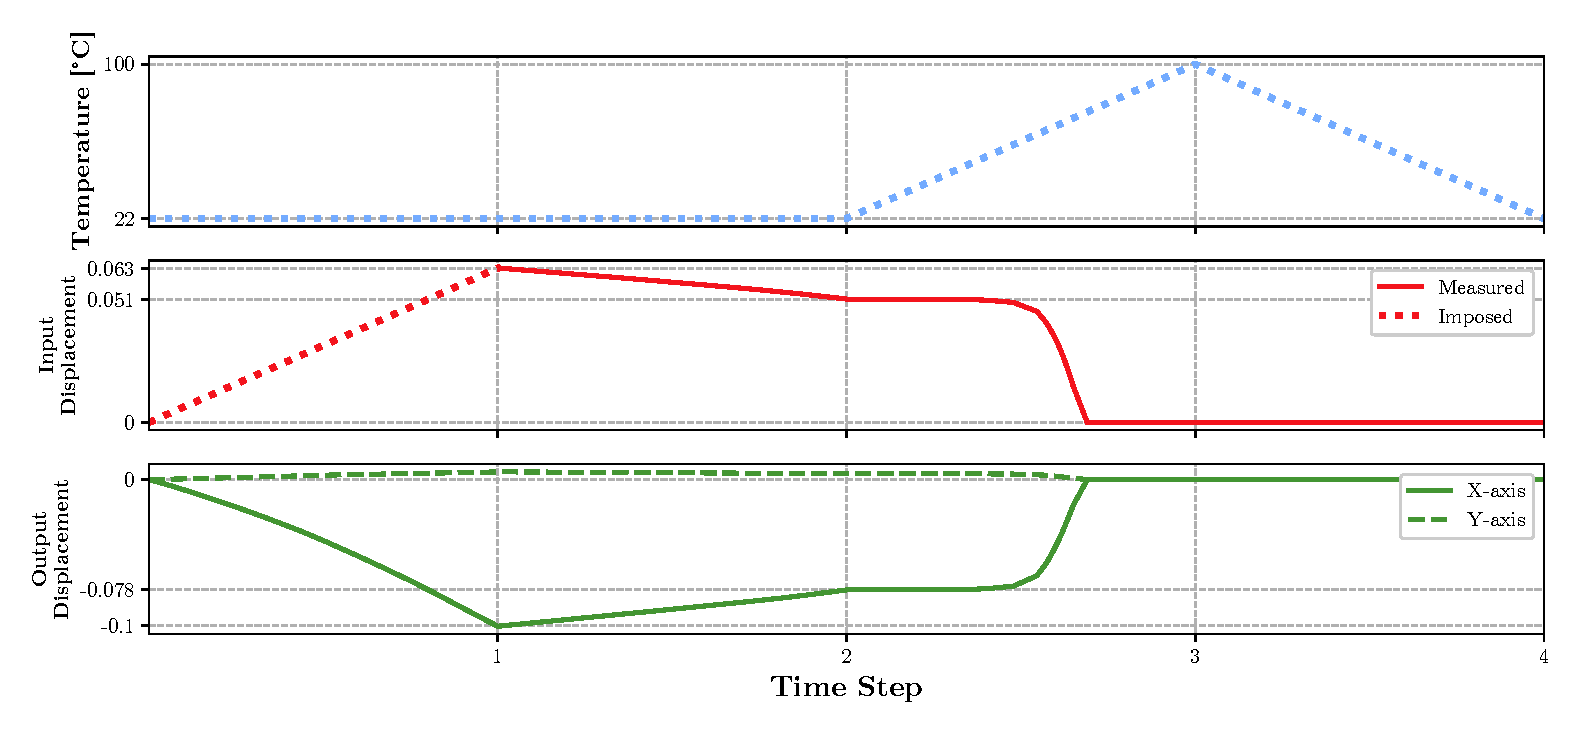
\includegraphics[width=\textwidth]{images/chap5/BM_Inverter30.eps}};
    \begin{scope}[x={(graph.south east)},y={(graph.north west)}]
    % \coordinate (ts0) at (1.54,7.6);
    % \coordinate (ts4) at (17.55,7.6);
    \coordinate (ts0) at (0.089,0.945);
    \coordinate (ts4) at (0.985,0.945);
    \coordinate (ts1) at ($ (ts0)!0.25!(ts4) $);
    \coordinate (ts2) at ($ (ts0)!0.5!(ts4) $);
    \coordinate (ts3) at ($ (ts0)!0.75!(ts4) $);
    \node[anchor=mid,inner sep=0] (ls0) at ($(ts0)!0.5!(ts1) + (0,0.05) $) {\fbox{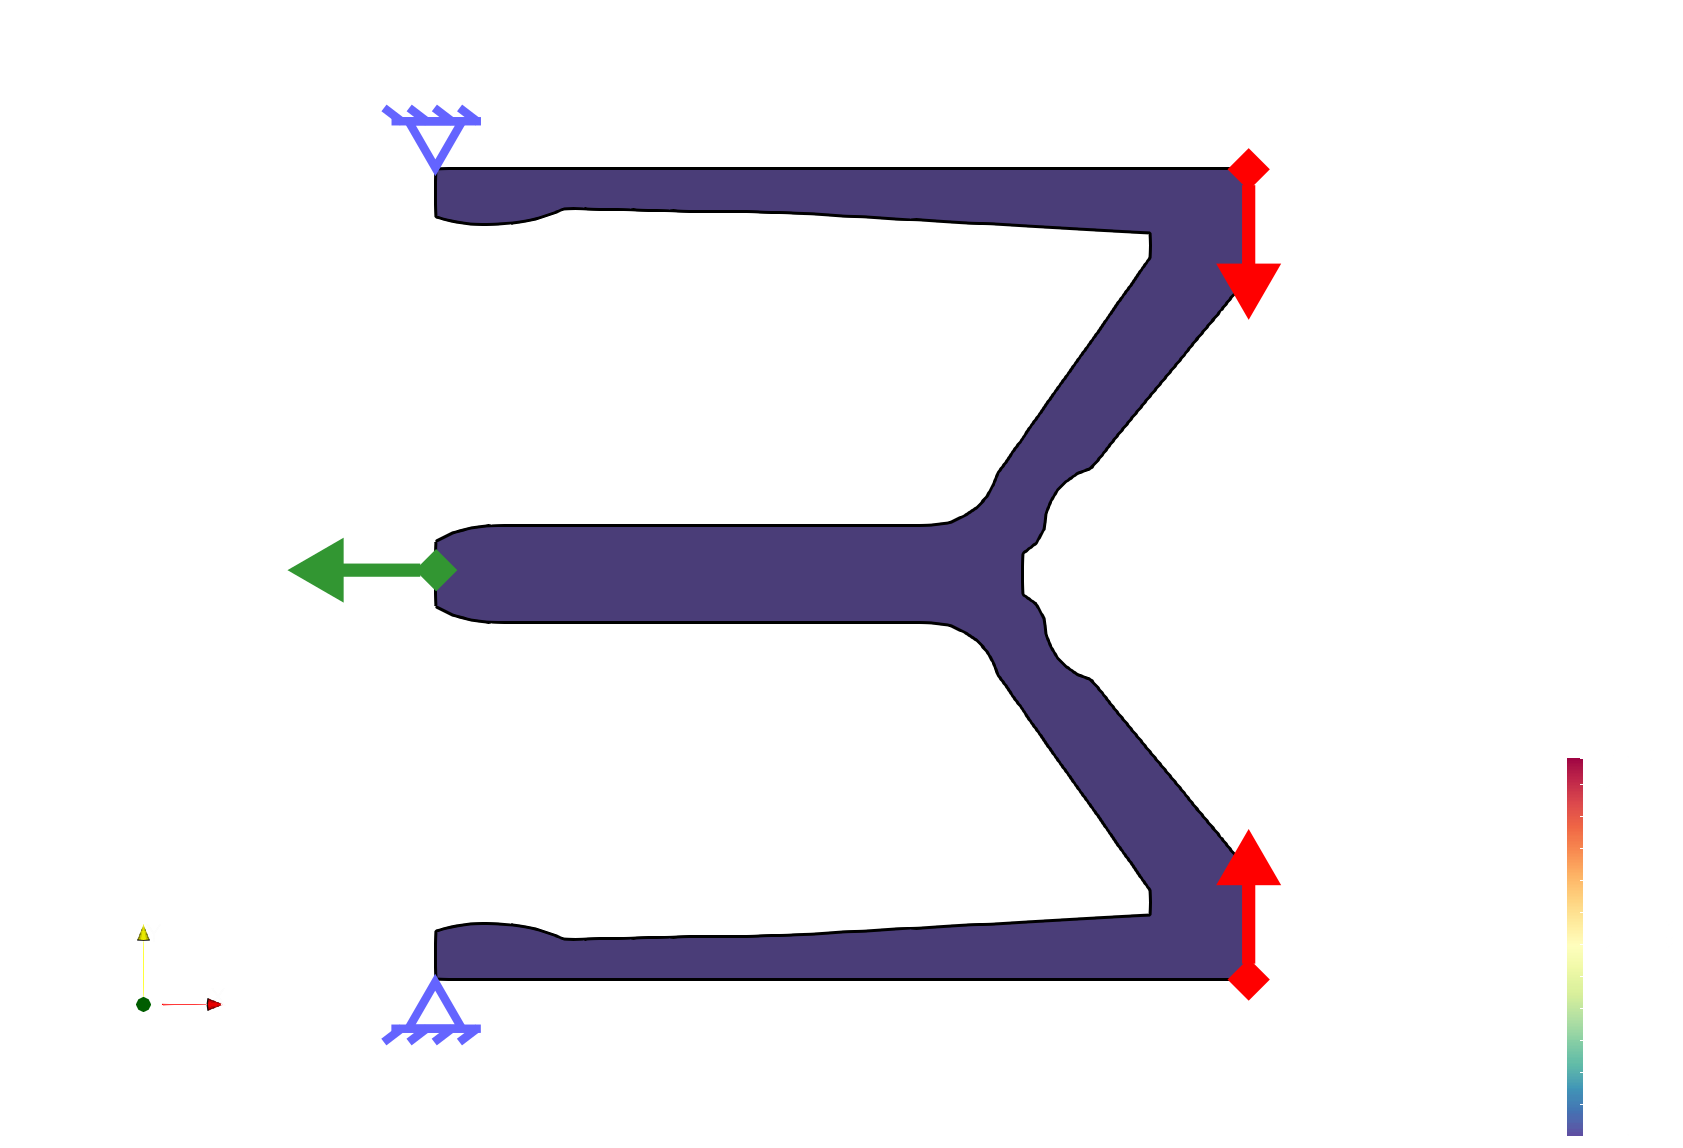
\includegraphics[height = 2cm,trim={11cm 3cm 13cm 3cm},clip]{images/chap5/Crimper_step0_v3.png}}};
    \draw[black, thick, -latex](ls0.west) to [bend right] (ts0);
    \node[anchor=mid,inner sep=0] (ls1) at ($(ts1)!0.5!(ts2) + (0,0.05) $) {\fbox{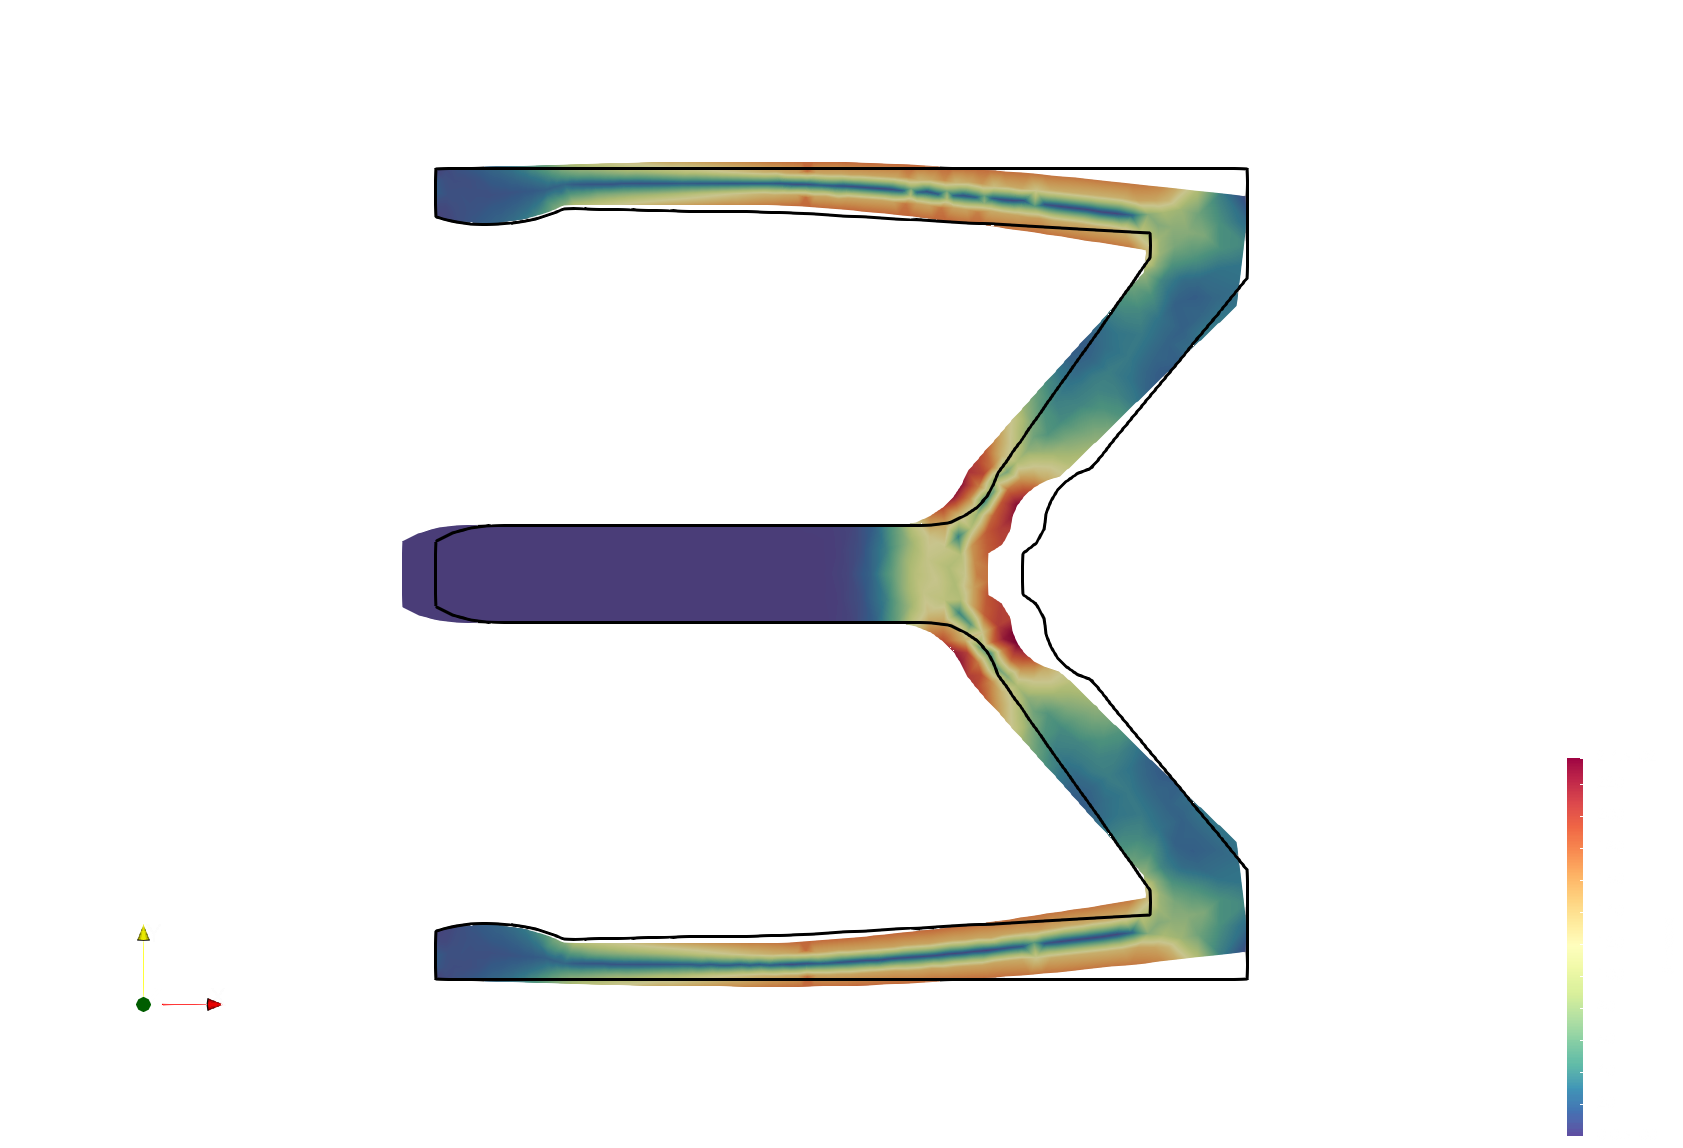
\includegraphics[height = 2cm,trim={11cm 3cm 13cm 3cm},clip]{images/chap5/Crimper_step1.png}}};
    \draw[black, thick, -latex](ls1.west) to [bend right] (ts1);
    \node[anchor=mid,inner sep=0] (ls2) at ($(ts2)!0.5!(ts3) + (0,0.05) $) {\fbox{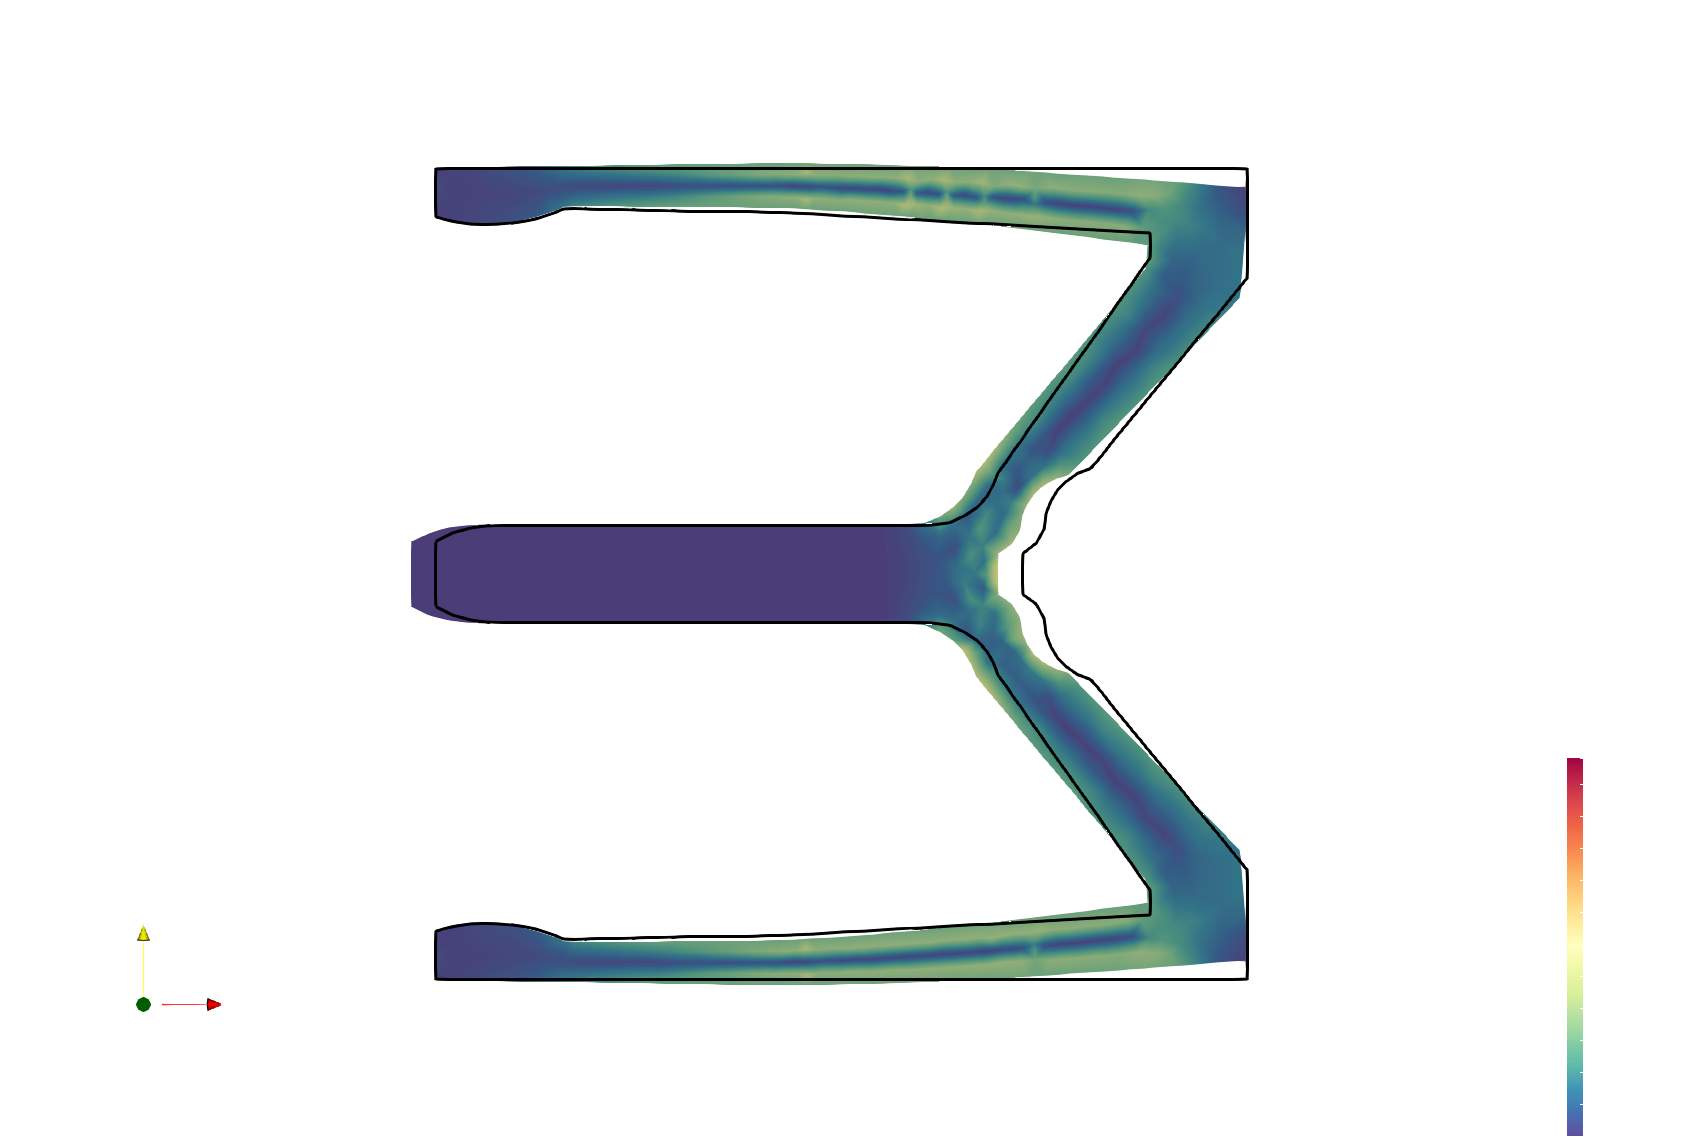
\includegraphics[height = 2cm,trim={11cm 3cm 13cm 3cm},clip]{images/chap5/Crimper_step2.png}}};
    \draw[black, thick, -latex](ls2.west) to [bend right] (ts2);
    \node[anchor=mid,inner sep=0] (ls3) at ($(ts3)!0.5!(ts4) + (0,0.05) $) {\fbox{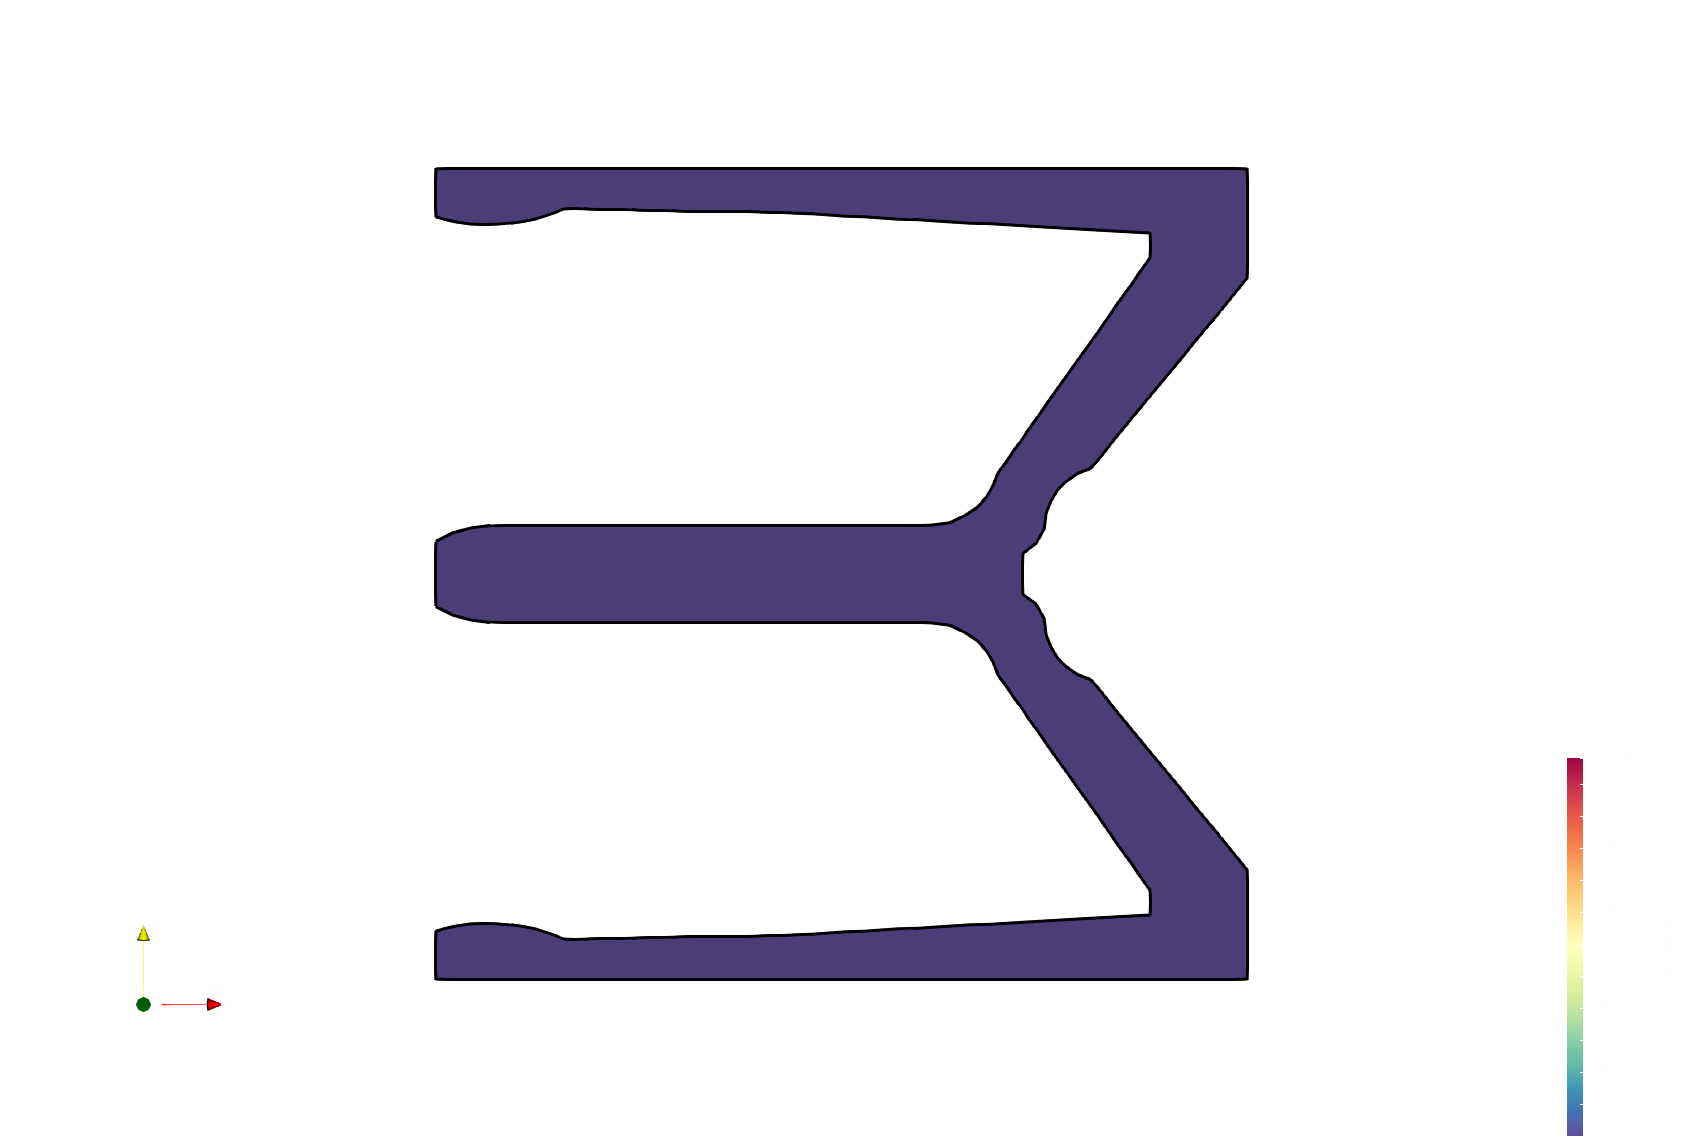
\includegraphics[height = 2cm,trim={11cm 3cm 13cm 3cm},clip]{images/chap5/Crimper_step0.png}}};
    \draw[black, thick, -latex](ls3.west) to [bend right] (ts3);
    \node[anchor=south east,inner sep=0] (ls0) at ($(ts4) + (0,0.015) $) {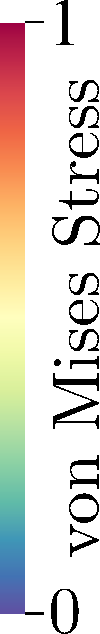
\includegraphics[height = 2.3cm]{images/chap5/Colorbar.pdf}};
    \end{scope}
    \end{tikzpicture}%
\end{document}

    \caption{Results of the shape memory effect simulation of the Crimper design showing a strain retention of $\alpha_\epsilon$ = 75.2\%.}
    \label{fig:CrimperAnsysSimu}
\end{figure}

\begin{figure}[hbt!]
    \centering
    % !TEX root = ../sethomas_thesis_main.tex
\documentclass[border=1mm,
               class=article
               preview]{standalone}
\usepackage{tikz}
\begin{document}
\begin{tikzpicture}
    \node[anchor=south west,inner sep=0] (graph) at (0,0) {\resizebox{\columnwidth}{!}{%% Creator: Matplotlib, PGF backend
%%
%% To include the figure in your LaTeX document, write
%%   \input{<filename>.pgf}
%%
%% Make sure the required packages are loaded in your preamble
%%   \usepackage{pgf}
%%
%% and, on pdftex
%%   \usepackage[utf8]{inputenc}\DeclareUnicodeCharacter{2212}{-}
%%
%% or, on luatex and xetex
%%   \usepackage{unicode-math}
%%
%% Figures using additional raster images can only be included by \input if
%% they are in the same directory as the main LaTeX file. For loading figures
%% from other directories you can use the `import` package
%%   \usepackage{import}
%%
%% and then include the figures with
%%   \import{<path to file>}{<filename>.pgf}
%%
%% Matplotlib used the following preamble
%%
\begingroup%
\makeatletter%
\begin{pgfpicture}%
\pgfpathrectangle{\pgfpointorigin}{\pgfqpoint{8.602007in}{4.649344in}}%
\pgfusepath{use as bounding box, clip}%
\begin{pgfscope}%
\pgfsetbuttcap%
\pgfsetmiterjoin%
\pgfsetlinewidth{0.000000pt}%
\definecolor{currentstroke}{rgb}{0.000000,0.000000,0.000000}%
\pgfsetstrokecolor{currentstroke}%
\pgfsetstrokeopacity{0.000000}%
\pgfsetdash{}{0pt}%
\pgfpathmoveto{\pgfqpoint{0.000000in}{0.000000in}}%
\pgfpathlineto{\pgfqpoint{8.602007in}{0.000000in}}%
\pgfpathlineto{\pgfqpoint{8.602007in}{4.649344in}}%
\pgfpathlineto{\pgfqpoint{0.000000in}{4.649344in}}%
\pgfpathclose%
\pgfusepath{}%
\end{pgfscope}%
\begin{pgfscope}%
\pgfsetbuttcap%
\pgfsetmiterjoin%
\pgfsetlinewidth{0.000000pt}%
\definecolor{currentstroke}{rgb}{0.000000,0.000000,0.000000}%
\pgfsetstrokecolor{currentstroke}%
\pgfsetstrokeopacity{0.000000}%
\pgfsetdash{}{0pt}%
\pgfpathmoveto{\pgfqpoint{0.717284in}{3.271659in}}%
\pgfpathlineto{\pgfqpoint{8.467284in}{3.271659in}}%
\pgfpathlineto{\pgfqpoint{8.467284in}{4.404012in}}%
\pgfpathlineto{\pgfqpoint{0.717284in}{4.404012in}}%
\pgfpathclose%
\pgfusepath{}%
\end{pgfscope}%
\begin{pgfscope}%
\pgfpathrectangle{\pgfqpoint{0.717284in}{3.271659in}}{\pgfqpoint{7.750000in}{1.132353in}}%
\pgfusepath{clip}%
\pgfsetbuttcap%
\pgfsetroundjoin%
\pgfsetlinewidth{0.803000pt}%
\definecolor{currentstroke}{rgb}{0.690196,0.690196,0.690196}%
\pgfsetstrokecolor{currentstroke}%
\pgfsetdash{{2.960000pt}{1.280000pt}}{0.000000pt}%
\pgfpathmoveto{\pgfqpoint{2.654784in}{3.271659in}}%
\pgfpathlineto{\pgfqpoint{2.654784in}{4.404012in}}%
\pgfusepath{stroke}%
\end{pgfscope}%
\begin{pgfscope}%
\pgfsetbuttcap%
\pgfsetroundjoin%
\definecolor{currentfill}{rgb}{0.000000,0.000000,0.000000}%
\pgfsetfillcolor{currentfill}%
\pgfsetlinewidth{0.803000pt}%
\definecolor{currentstroke}{rgb}{0.000000,0.000000,0.000000}%
\pgfsetstrokecolor{currentstroke}%
\pgfsetdash{}{0pt}%
\pgfsys@defobject{currentmarker}{\pgfqpoint{0.000000in}{-0.048611in}}{\pgfqpoint{0.000000in}{0.000000in}}{%
\pgfpathmoveto{\pgfqpoint{0.000000in}{0.000000in}}%
\pgfpathlineto{\pgfqpoint{0.000000in}{-0.048611in}}%
\pgfusepath{stroke,fill}%
}%
\begin{pgfscope}%
\pgfsys@transformshift{2.654784in}{3.271659in}%
\pgfsys@useobject{currentmarker}{}%
\end{pgfscope}%
\end{pgfscope}%
\begin{pgfscope}%
\pgfpathrectangle{\pgfqpoint{0.717284in}{3.271659in}}{\pgfqpoint{7.750000in}{1.132353in}}%
\pgfusepath{clip}%
\pgfsetbuttcap%
\pgfsetroundjoin%
\pgfsetlinewidth{0.803000pt}%
\definecolor{currentstroke}{rgb}{0.690196,0.690196,0.690196}%
\pgfsetstrokecolor{currentstroke}%
\pgfsetdash{{2.960000pt}{1.280000pt}}{0.000000pt}%
\pgfpathmoveto{\pgfqpoint{4.592284in}{3.271659in}}%
\pgfpathlineto{\pgfqpoint{4.592284in}{4.404012in}}%
\pgfusepath{stroke}%
\end{pgfscope}%
\begin{pgfscope}%
\pgfsetbuttcap%
\pgfsetroundjoin%
\definecolor{currentfill}{rgb}{0.000000,0.000000,0.000000}%
\pgfsetfillcolor{currentfill}%
\pgfsetlinewidth{0.803000pt}%
\definecolor{currentstroke}{rgb}{0.000000,0.000000,0.000000}%
\pgfsetstrokecolor{currentstroke}%
\pgfsetdash{}{0pt}%
\pgfsys@defobject{currentmarker}{\pgfqpoint{0.000000in}{-0.048611in}}{\pgfqpoint{0.000000in}{0.000000in}}{%
\pgfpathmoveto{\pgfqpoint{0.000000in}{0.000000in}}%
\pgfpathlineto{\pgfqpoint{0.000000in}{-0.048611in}}%
\pgfusepath{stroke,fill}%
}%
\begin{pgfscope}%
\pgfsys@transformshift{4.592284in}{3.271659in}%
\pgfsys@useobject{currentmarker}{}%
\end{pgfscope}%
\end{pgfscope}%
\begin{pgfscope}%
\pgfpathrectangle{\pgfqpoint{0.717284in}{3.271659in}}{\pgfqpoint{7.750000in}{1.132353in}}%
\pgfusepath{clip}%
\pgfsetbuttcap%
\pgfsetroundjoin%
\pgfsetlinewidth{0.803000pt}%
\definecolor{currentstroke}{rgb}{0.690196,0.690196,0.690196}%
\pgfsetstrokecolor{currentstroke}%
\pgfsetdash{{2.960000pt}{1.280000pt}}{0.000000pt}%
\pgfpathmoveto{\pgfqpoint{6.529784in}{3.271659in}}%
\pgfpathlineto{\pgfqpoint{6.529784in}{4.404012in}}%
\pgfusepath{stroke}%
\end{pgfscope}%
\begin{pgfscope}%
\pgfsetbuttcap%
\pgfsetroundjoin%
\definecolor{currentfill}{rgb}{0.000000,0.000000,0.000000}%
\pgfsetfillcolor{currentfill}%
\pgfsetlinewidth{0.803000pt}%
\definecolor{currentstroke}{rgb}{0.000000,0.000000,0.000000}%
\pgfsetstrokecolor{currentstroke}%
\pgfsetdash{}{0pt}%
\pgfsys@defobject{currentmarker}{\pgfqpoint{0.000000in}{-0.048611in}}{\pgfqpoint{0.000000in}{0.000000in}}{%
\pgfpathmoveto{\pgfqpoint{0.000000in}{0.000000in}}%
\pgfpathlineto{\pgfqpoint{0.000000in}{-0.048611in}}%
\pgfusepath{stroke,fill}%
}%
\begin{pgfscope}%
\pgfsys@transformshift{6.529784in}{3.271659in}%
\pgfsys@useobject{currentmarker}{}%
\end{pgfscope}%
\end{pgfscope}%
\begin{pgfscope}%
\pgfpathrectangle{\pgfqpoint{0.717284in}{3.271659in}}{\pgfqpoint{7.750000in}{1.132353in}}%
\pgfusepath{clip}%
\pgfsetbuttcap%
\pgfsetroundjoin%
\pgfsetlinewidth{0.803000pt}%
\definecolor{currentstroke}{rgb}{0.690196,0.690196,0.690196}%
\pgfsetstrokecolor{currentstroke}%
\pgfsetdash{{2.960000pt}{1.280000pt}}{0.000000pt}%
\pgfpathmoveto{\pgfqpoint{8.467284in}{3.271659in}}%
\pgfpathlineto{\pgfqpoint{8.467284in}{4.404012in}}%
\pgfusepath{stroke}%
\end{pgfscope}%
\begin{pgfscope}%
\pgfsetbuttcap%
\pgfsetroundjoin%
\definecolor{currentfill}{rgb}{0.000000,0.000000,0.000000}%
\pgfsetfillcolor{currentfill}%
\pgfsetlinewidth{0.803000pt}%
\definecolor{currentstroke}{rgb}{0.000000,0.000000,0.000000}%
\pgfsetstrokecolor{currentstroke}%
\pgfsetdash{}{0pt}%
\pgfsys@defobject{currentmarker}{\pgfqpoint{0.000000in}{-0.048611in}}{\pgfqpoint{0.000000in}{0.000000in}}{%
\pgfpathmoveto{\pgfqpoint{0.000000in}{0.000000in}}%
\pgfpathlineto{\pgfqpoint{0.000000in}{-0.048611in}}%
\pgfusepath{stroke,fill}%
}%
\begin{pgfscope}%
\pgfsys@transformshift{8.467284in}{3.271659in}%
\pgfsys@useobject{currentmarker}{}%
\end{pgfscope}%
\end{pgfscope}%
\begin{pgfscope}%
\pgfpathrectangle{\pgfqpoint{0.717284in}{3.271659in}}{\pgfqpoint{7.750000in}{1.132353in}}%
\pgfusepath{clip}%
\pgfsetbuttcap%
\pgfsetroundjoin%
\pgfsetlinewidth{0.803000pt}%
\definecolor{currentstroke}{rgb}{0.690196,0.690196,0.690196}%
\pgfsetstrokecolor{currentstroke}%
\pgfsetdash{{2.960000pt}{1.280000pt}}{0.000000pt}%
\pgfpathmoveto{\pgfqpoint{0.717284in}{3.323129in}}%
\pgfpathlineto{\pgfqpoint{8.467284in}{3.323129in}}%
\pgfusepath{stroke}%
\end{pgfscope}%
\begin{pgfscope}%
\pgfsetbuttcap%
\pgfsetroundjoin%
\definecolor{currentfill}{rgb}{0.000000,0.000000,0.000000}%
\pgfsetfillcolor{currentfill}%
\pgfsetlinewidth{0.803000pt}%
\definecolor{currentstroke}{rgb}{0.000000,0.000000,0.000000}%
\pgfsetstrokecolor{currentstroke}%
\pgfsetdash{}{0pt}%
\pgfsys@defobject{currentmarker}{\pgfqpoint{-0.048611in}{0.000000in}}{\pgfqpoint{-0.000000in}{0.000000in}}{%
\pgfpathmoveto{\pgfqpoint{-0.000000in}{0.000000in}}%
\pgfpathlineto{\pgfqpoint{-0.048611in}{0.000000in}}%
\pgfusepath{stroke,fill}%
}%
\begin{pgfscope}%
\pgfsys@transformshift{0.717284in}{3.323129in}%
\pgfsys@useobject{currentmarker}{}%
\end{pgfscope}%
\end{pgfscope}%
\begin{pgfscope}%
\definecolor{textcolor}{rgb}{0.000000,0.000000,0.000000}%
\pgfsetstrokecolor{textcolor}%
\pgfsetfillcolor{textcolor}%
\pgftext[x=0.481173in, y=3.274904in, left, base]{\color{textcolor}\rmfamily\fontsize{10.000000}{12.000000}\selectfont \(\displaystyle {22}\)}%
\end{pgfscope}%
\begin{pgfscope}%
\pgfpathrectangle{\pgfqpoint{0.717284in}{3.271659in}}{\pgfqpoint{7.750000in}{1.132353in}}%
\pgfusepath{clip}%
\pgfsetbuttcap%
\pgfsetroundjoin%
\pgfsetlinewidth{0.803000pt}%
\definecolor{currentstroke}{rgb}{0.690196,0.690196,0.690196}%
\pgfsetstrokecolor{currentstroke}%
\pgfsetdash{{2.960000pt}{1.280000pt}}{0.000000pt}%
\pgfpathmoveto{\pgfqpoint{0.717284in}{4.352541in}}%
\pgfpathlineto{\pgfqpoint{8.467284in}{4.352541in}}%
\pgfusepath{stroke}%
\end{pgfscope}%
\begin{pgfscope}%
\pgfsetbuttcap%
\pgfsetroundjoin%
\definecolor{currentfill}{rgb}{0.000000,0.000000,0.000000}%
\pgfsetfillcolor{currentfill}%
\pgfsetlinewidth{0.803000pt}%
\definecolor{currentstroke}{rgb}{0.000000,0.000000,0.000000}%
\pgfsetstrokecolor{currentstroke}%
\pgfsetdash{}{0pt}%
\pgfsys@defobject{currentmarker}{\pgfqpoint{-0.048611in}{0.000000in}}{\pgfqpoint{-0.000000in}{0.000000in}}{%
\pgfpathmoveto{\pgfqpoint{-0.000000in}{0.000000in}}%
\pgfpathlineto{\pgfqpoint{-0.048611in}{0.000000in}}%
\pgfusepath{stroke,fill}%
}%
\begin{pgfscope}%
\pgfsys@transformshift{0.717284in}{4.352541in}%
\pgfsys@useobject{currentmarker}{}%
\end{pgfscope}%
\end{pgfscope}%
\begin{pgfscope}%
\definecolor{textcolor}{rgb}{0.000000,0.000000,0.000000}%
\pgfsetstrokecolor{textcolor}%
\pgfsetfillcolor{textcolor}%
\pgftext[x=0.411728in, y=4.304316in, left, base]{\color{textcolor}\rmfamily\fontsize{10.000000}{12.000000}\selectfont \(\displaystyle {160}\)}%
\end{pgfscope}%
\begin{pgfscope}%
\definecolor{textcolor}{rgb}{0.000000,0.000000,0.000000}%
\pgfsetstrokecolor{textcolor}%
\pgfsetfillcolor{textcolor}%
\pgftext[x=0.356173in,y=3.837835in,,bottom,rotate=90.000000]{\color{textcolor}\rmfamily\fontsize{12.000000}{14.400000}\bfseries\selectfont Temperature [°C]}%
\end{pgfscope}%
\begin{pgfscope}%
\pgfpathrectangle{\pgfqpoint{0.717284in}{3.271659in}}{\pgfqpoint{7.750000in}{1.132353in}}%
\pgfusepath{clip}%
\pgfsetbuttcap%
\pgfsetroundjoin%
\pgfsetlinewidth{3.011250pt}%
\definecolor{currentstroke}{rgb}{0.450980,0.670588,1.000000}%
\pgfsetstrokecolor{currentstroke}%
\pgfsetdash{{3.000000pt}{4.950000pt}}{0.000000pt}%
\pgfpathmoveto{\pgfqpoint{0.717284in}{3.323129in}}%
\pgfpathlineto{\pgfqpoint{4.592284in}{3.323129in}}%
\pgfpathlineto{\pgfqpoint{5.756528in}{3.941672in}}%
\pgfpathlineto{\pgfqpoint{5.756916in}{3.941672in}}%
\pgfpathlineto{\pgfqpoint{6.529784in}{4.352541in}}%
\pgfpathlineto{\pgfqpoint{8.467284in}{3.323129in}}%
\pgfpathlineto{\pgfqpoint{8.467284in}{3.323129in}}%
\pgfusepath{stroke}%
\end{pgfscope}%
\begin{pgfscope}%
\pgfsetrectcap%
\pgfsetmiterjoin%
\pgfsetlinewidth{0.803000pt}%
\definecolor{currentstroke}{rgb}{0.000000,0.000000,0.000000}%
\pgfsetstrokecolor{currentstroke}%
\pgfsetdash{}{0pt}%
\pgfpathmoveto{\pgfqpoint{0.717284in}{3.271659in}}%
\pgfpathlineto{\pgfqpoint{0.717284in}{4.404012in}}%
\pgfusepath{stroke}%
\end{pgfscope}%
\begin{pgfscope}%
\pgfsetrectcap%
\pgfsetmiterjoin%
\pgfsetlinewidth{0.803000pt}%
\definecolor{currentstroke}{rgb}{0.000000,0.000000,0.000000}%
\pgfsetstrokecolor{currentstroke}%
\pgfsetdash{}{0pt}%
\pgfpathmoveto{\pgfqpoint{8.467284in}{3.271659in}}%
\pgfpathlineto{\pgfqpoint{8.467284in}{4.404012in}}%
\pgfusepath{stroke}%
\end{pgfscope}%
\begin{pgfscope}%
\pgfsetrectcap%
\pgfsetmiterjoin%
\pgfsetlinewidth{0.803000pt}%
\definecolor{currentstroke}{rgb}{0.000000,0.000000,0.000000}%
\pgfsetstrokecolor{currentstroke}%
\pgfsetdash{}{0pt}%
\pgfpathmoveto{\pgfqpoint{0.717284in}{3.271659in}}%
\pgfpathlineto{\pgfqpoint{8.467284in}{3.271659in}}%
\pgfusepath{stroke}%
\end{pgfscope}%
\begin{pgfscope}%
\pgfsetrectcap%
\pgfsetmiterjoin%
\pgfsetlinewidth{0.803000pt}%
\definecolor{currentstroke}{rgb}{0.000000,0.000000,0.000000}%
\pgfsetstrokecolor{currentstroke}%
\pgfsetdash{}{0pt}%
\pgfpathmoveto{\pgfqpoint{0.717284in}{4.404012in}}%
\pgfpathlineto{\pgfqpoint{8.467284in}{4.404012in}}%
\pgfusepath{stroke}%
\end{pgfscope}%
\begin{pgfscope}%
\pgfsetbuttcap%
\pgfsetmiterjoin%
\pgfsetlinewidth{0.000000pt}%
\definecolor{currentstroke}{rgb}{0.000000,0.000000,0.000000}%
\pgfsetstrokecolor{currentstroke}%
\pgfsetstrokeopacity{0.000000}%
\pgfsetdash{}{0pt}%
\pgfpathmoveto{\pgfqpoint{0.717284in}{1.912835in}}%
\pgfpathlineto{\pgfqpoint{8.467284in}{1.912835in}}%
\pgfpathlineto{\pgfqpoint{8.467284in}{3.045188in}}%
\pgfpathlineto{\pgfqpoint{0.717284in}{3.045188in}}%
\pgfpathclose%
\pgfusepath{}%
\end{pgfscope}%
\begin{pgfscope}%
\pgfpathrectangle{\pgfqpoint{0.717284in}{1.912835in}}{\pgfqpoint{7.750000in}{1.132353in}}%
\pgfusepath{clip}%
\pgfsetbuttcap%
\pgfsetroundjoin%
\pgfsetlinewidth{0.803000pt}%
\definecolor{currentstroke}{rgb}{0.690196,0.690196,0.690196}%
\pgfsetstrokecolor{currentstroke}%
\pgfsetdash{{2.960000pt}{1.280000pt}}{0.000000pt}%
\pgfpathmoveto{\pgfqpoint{2.654784in}{1.912835in}}%
\pgfpathlineto{\pgfqpoint{2.654784in}{3.045188in}}%
\pgfusepath{stroke}%
\end{pgfscope}%
\begin{pgfscope}%
\pgfsetbuttcap%
\pgfsetroundjoin%
\definecolor{currentfill}{rgb}{0.000000,0.000000,0.000000}%
\pgfsetfillcolor{currentfill}%
\pgfsetlinewidth{0.803000pt}%
\definecolor{currentstroke}{rgb}{0.000000,0.000000,0.000000}%
\pgfsetstrokecolor{currentstroke}%
\pgfsetdash{}{0pt}%
\pgfsys@defobject{currentmarker}{\pgfqpoint{0.000000in}{-0.048611in}}{\pgfqpoint{0.000000in}{0.000000in}}{%
\pgfpathmoveto{\pgfqpoint{0.000000in}{0.000000in}}%
\pgfpathlineto{\pgfqpoint{0.000000in}{-0.048611in}}%
\pgfusepath{stroke,fill}%
}%
\begin{pgfscope}%
\pgfsys@transformshift{2.654784in}{1.912835in}%
\pgfsys@useobject{currentmarker}{}%
\end{pgfscope}%
\end{pgfscope}%
\begin{pgfscope}%
\pgfpathrectangle{\pgfqpoint{0.717284in}{1.912835in}}{\pgfqpoint{7.750000in}{1.132353in}}%
\pgfusepath{clip}%
\pgfsetbuttcap%
\pgfsetroundjoin%
\pgfsetlinewidth{0.803000pt}%
\definecolor{currentstroke}{rgb}{0.690196,0.690196,0.690196}%
\pgfsetstrokecolor{currentstroke}%
\pgfsetdash{{2.960000pt}{1.280000pt}}{0.000000pt}%
\pgfpathmoveto{\pgfqpoint{4.592284in}{1.912835in}}%
\pgfpathlineto{\pgfqpoint{4.592284in}{3.045188in}}%
\pgfusepath{stroke}%
\end{pgfscope}%
\begin{pgfscope}%
\pgfsetbuttcap%
\pgfsetroundjoin%
\definecolor{currentfill}{rgb}{0.000000,0.000000,0.000000}%
\pgfsetfillcolor{currentfill}%
\pgfsetlinewidth{0.803000pt}%
\definecolor{currentstroke}{rgb}{0.000000,0.000000,0.000000}%
\pgfsetstrokecolor{currentstroke}%
\pgfsetdash{}{0pt}%
\pgfsys@defobject{currentmarker}{\pgfqpoint{0.000000in}{-0.048611in}}{\pgfqpoint{0.000000in}{0.000000in}}{%
\pgfpathmoveto{\pgfqpoint{0.000000in}{0.000000in}}%
\pgfpathlineto{\pgfqpoint{0.000000in}{-0.048611in}}%
\pgfusepath{stroke,fill}%
}%
\begin{pgfscope}%
\pgfsys@transformshift{4.592284in}{1.912835in}%
\pgfsys@useobject{currentmarker}{}%
\end{pgfscope}%
\end{pgfscope}%
\begin{pgfscope}%
\pgfpathrectangle{\pgfqpoint{0.717284in}{1.912835in}}{\pgfqpoint{7.750000in}{1.132353in}}%
\pgfusepath{clip}%
\pgfsetbuttcap%
\pgfsetroundjoin%
\pgfsetlinewidth{0.803000pt}%
\definecolor{currentstroke}{rgb}{0.690196,0.690196,0.690196}%
\pgfsetstrokecolor{currentstroke}%
\pgfsetdash{{2.960000pt}{1.280000pt}}{0.000000pt}%
\pgfpathmoveto{\pgfqpoint{6.529784in}{1.912835in}}%
\pgfpathlineto{\pgfqpoint{6.529784in}{3.045188in}}%
\pgfusepath{stroke}%
\end{pgfscope}%
\begin{pgfscope}%
\pgfsetbuttcap%
\pgfsetroundjoin%
\definecolor{currentfill}{rgb}{0.000000,0.000000,0.000000}%
\pgfsetfillcolor{currentfill}%
\pgfsetlinewidth{0.803000pt}%
\definecolor{currentstroke}{rgb}{0.000000,0.000000,0.000000}%
\pgfsetstrokecolor{currentstroke}%
\pgfsetdash{}{0pt}%
\pgfsys@defobject{currentmarker}{\pgfqpoint{0.000000in}{-0.048611in}}{\pgfqpoint{0.000000in}{0.000000in}}{%
\pgfpathmoveto{\pgfqpoint{0.000000in}{0.000000in}}%
\pgfpathlineto{\pgfqpoint{0.000000in}{-0.048611in}}%
\pgfusepath{stroke,fill}%
}%
\begin{pgfscope}%
\pgfsys@transformshift{6.529784in}{1.912835in}%
\pgfsys@useobject{currentmarker}{}%
\end{pgfscope}%
\end{pgfscope}%
\begin{pgfscope}%
\pgfpathrectangle{\pgfqpoint{0.717284in}{1.912835in}}{\pgfqpoint{7.750000in}{1.132353in}}%
\pgfusepath{clip}%
\pgfsetbuttcap%
\pgfsetroundjoin%
\pgfsetlinewidth{0.803000pt}%
\definecolor{currentstroke}{rgb}{0.690196,0.690196,0.690196}%
\pgfsetstrokecolor{currentstroke}%
\pgfsetdash{{2.960000pt}{1.280000pt}}{0.000000pt}%
\pgfpathmoveto{\pgfqpoint{8.467284in}{1.912835in}}%
\pgfpathlineto{\pgfqpoint{8.467284in}{3.045188in}}%
\pgfusepath{stroke}%
\end{pgfscope}%
\begin{pgfscope}%
\pgfsetbuttcap%
\pgfsetroundjoin%
\definecolor{currentfill}{rgb}{0.000000,0.000000,0.000000}%
\pgfsetfillcolor{currentfill}%
\pgfsetlinewidth{0.803000pt}%
\definecolor{currentstroke}{rgb}{0.000000,0.000000,0.000000}%
\pgfsetstrokecolor{currentstroke}%
\pgfsetdash{}{0pt}%
\pgfsys@defobject{currentmarker}{\pgfqpoint{0.000000in}{-0.048611in}}{\pgfqpoint{0.000000in}{0.000000in}}{%
\pgfpathmoveto{\pgfqpoint{0.000000in}{0.000000in}}%
\pgfpathlineto{\pgfqpoint{0.000000in}{-0.048611in}}%
\pgfusepath{stroke,fill}%
}%
\begin{pgfscope}%
\pgfsys@transformshift{8.467284in}{1.912835in}%
\pgfsys@useobject{currentmarker}{}%
\end{pgfscope}%
\end{pgfscope}%
\begin{pgfscope}%
\pgfpathrectangle{\pgfqpoint{0.717284in}{1.912835in}}{\pgfqpoint{7.750000in}{1.132353in}}%
\pgfusepath{clip}%
\pgfsetbuttcap%
\pgfsetroundjoin%
\pgfsetlinewidth{0.803000pt}%
\definecolor{currentstroke}{rgb}{0.690196,0.690196,0.690196}%
\pgfsetstrokecolor{currentstroke}%
\pgfsetdash{{2.960000pt}{1.280000pt}}{0.000000pt}%
\pgfpathmoveto{\pgfqpoint{0.717284in}{1.964306in}}%
\pgfpathlineto{\pgfqpoint{8.467284in}{1.964306in}}%
\pgfusepath{stroke}%
\end{pgfscope}%
\begin{pgfscope}%
\pgfsetbuttcap%
\pgfsetroundjoin%
\definecolor{currentfill}{rgb}{0.000000,0.000000,0.000000}%
\pgfsetfillcolor{currentfill}%
\pgfsetlinewidth{0.803000pt}%
\definecolor{currentstroke}{rgb}{0.000000,0.000000,0.000000}%
\pgfsetstrokecolor{currentstroke}%
\pgfsetdash{}{0pt}%
\pgfsys@defobject{currentmarker}{\pgfqpoint{-0.048611in}{0.000000in}}{\pgfqpoint{-0.000000in}{0.000000in}}{%
\pgfpathmoveto{\pgfqpoint{-0.000000in}{0.000000in}}%
\pgfpathlineto{\pgfqpoint{-0.048611in}{0.000000in}}%
\pgfusepath{stroke,fill}%
}%
\begin{pgfscope}%
\pgfsys@transformshift{0.717284in}{1.964306in}%
\pgfsys@useobject{currentmarker}{}%
\end{pgfscope}%
\end{pgfscope}%
\begin{pgfscope}%
\definecolor{textcolor}{rgb}{0.000000,0.000000,0.000000}%
\pgfsetstrokecolor{textcolor}%
\pgfsetfillcolor{textcolor}%
\pgftext[x=0.550617in, y=1.916081in, left, base]{\color{textcolor}\rmfamily\fontsize{10.000000}{12.000000}\selectfont 0}%
\end{pgfscope}%
\begin{pgfscope}%
\pgfpathrectangle{\pgfqpoint{0.717284in}{1.912835in}}{\pgfqpoint{7.750000in}{1.132353in}}%
\pgfusepath{clip}%
\pgfsetbuttcap%
\pgfsetroundjoin%
\pgfsetlinewidth{0.803000pt}%
\definecolor{currentstroke}{rgb}{0.690196,0.690196,0.690196}%
\pgfsetstrokecolor{currentstroke}%
\pgfsetdash{{2.960000pt}{1.280000pt}}{0.000000pt}%
\pgfpathmoveto{\pgfqpoint{0.717284in}{2.756387in}}%
\pgfpathlineto{\pgfqpoint{8.467284in}{2.756387in}}%
\pgfusepath{stroke}%
\end{pgfscope}%
\begin{pgfscope}%
\pgfsetbuttcap%
\pgfsetroundjoin%
\definecolor{currentfill}{rgb}{0.000000,0.000000,0.000000}%
\pgfsetfillcolor{currentfill}%
\pgfsetlinewidth{0.803000pt}%
\definecolor{currentstroke}{rgb}{0.000000,0.000000,0.000000}%
\pgfsetstrokecolor{currentstroke}%
\pgfsetdash{}{0pt}%
\pgfsys@defobject{currentmarker}{\pgfqpoint{-0.048611in}{0.000000in}}{\pgfqpoint{-0.000000in}{0.000000in}}{%
\pgfpathmoveto{\pgfqpoint{-0.000000in}{0.000000in}}%
\pgfpathlineto{\pgfqpoint{-0.048611in}{0.000000in}}%
\pgfusepath{stroke,fill}%
}%
\begin{pgfscope}%
\pgfsys@transformshift{0.717284in}{2.756387in}%
\pgfsys@useobject{currentmarker}{}%
\end{pgfscope}%
\end{pgfscope}%
\begin{pgfscope}%
\definecolor{textcolor}{rgb}{0.000000,0.000000,0.000000}%
\pgfsetstrokecolor{textcolor}%
\pgfsetfillcolor{textcolor}%
\pgftext[x=0.303703in, y=2.708162in, left, base]{\color{textcolor}\rmfamily\fontsize{10.000000}{12.000000}\selectfont 0.077}%
\end{pgfscope}%
\begin{pgfscope}%
\pgfpathrectangle{\pgfqpoint{0.717284in}{1.912835in}}{\pgfqpoint{7.750000in}{1.132353in}}%
\pgfusepath{clip}%
\pgfsetbuttcap%
\pgfsetroundjoin%
\pgfsetlinewidth{0.803000pt}%
\definecolor{currentstroke}{rgb}{0.690196,0.690196,0.690196}%
\pgfsetstrokecolor{currentstroke}%
\pgfsetdash{{2.960000pt}{1.280000pt}}{0.000000pt}%
\pgfpathmoveto{\pgfqpoint{0.717284in}{2.990866in}}%
\pgfpathlineto{\pgfqpoint{8.467284in}{2.990866in}}%
\pgfusepath{stroke}%
\end{pgfscope}%
\begin{pgfscope}%
\pgfsetbuttcap%
\pgfsetroundjoin%
\definecolor{currentfill}{rgb}{0.000000,0.000000,0.000000}%
\pgfsetfillcolor{currentfill}%
\pgfsetlinewidth{0.803000pt}%
\definecolor{currentstroke}{rgb}{0.000000,0.000000,0.000000}%
\pgfsetstrokecolor{currentstroke}%
\pgfsetdash{}{0pt}%
\pgfsys@defobject{currentmarker}{\pgfqpoint{-0.048611in}{0.000000in}}{\pgfqpoint{-0.000000in}{0.000000in}}{%
\pgfpathmoveto{\pgfqpoint{-0.000000in}{0.000000in}}%
\pgfpathlineto{\pgfqpoint{-0.048611in}{0.000000in}}%
\pgfusepath{stroke,fill}%
}%
\begin{pgfscope}%
\pgfsys@transformshift{0.717284in}{2.990866in}%
\pgfsys@useobject{currentmarker}{}%
\end{pgfscope}%
\end{pgfscope}%
\begin{pgfscope}%
\definecolor{textcolor}{rgb}{0.000000,0.000000,0.000000}%
\pgfsetstrokecolor{textcolor}%
\pgfsetfillcolor{textcolor}%
\pgftext[x=0.442592in, y=2.942641in, left, base]{\color{textcolor}\rmfamily\fontsize{10.000000}{12.000000}\selectfont 0.1}%
\end{pgfscope}%
\begin{pgfscope}%
\definecolor{textcolor}{rgb}{0.000000,0.000000,0.000000}%
\pgfsetstrokecolor{textcolor}%
\pgfsetfillcolor{textcolor}%
\pgftext[x=0.248148in,y=2.479012in,,bottom,rotate=90.000000]{\color{textcolor}\rmfamily\fontsize{12.000000}{14.400000}\bfseries\selectfont Input Strain}%
\end{pgfscope}%
\begin{pgfscope}%
\pgfpathrectangle{\pgfqpoint{0.717284in}{1.912835in}}{\pgfqpoint{7.750000in}{1.132353in}}%
\pgfusepath{clip}%
\pgfsetrectcap%
\pgfsetroundjoin%
\pgfsetlinewidth{2.007500pt}%
\definecolor{currentstroke}{rgb}{0.952941,0.078431,0.113725}%
\pgfsetstrokecolor{currentstroke}%
\pgfsetdash{}{0pt}%
\pgfpathmoveto{\pgfqpoint{2.667766in}{2.992277in}}%
\pgfpathlineto{\pgfqpoint{2.680553in}{2.990866in}}%
\pgfpathlineto{\pgfqpoint{2.699928in}{2.988735in}}%
\pgfpathlineto{\pgfqpoint{2.728991in}{2.985554in}}%
\pgfpathlineto{\pgfqpoint{2.772584in}{2.980768in}}%
\pgfpathlineto{\pgfqpoint{2.838072in}{2.973593in}}%
\pgfpathlineto{\pgfqpoint{2.936109in}{2.962804in}}%
\pgfpathlineto{\pgfqpoint{3.065341in}{2.948537in}}%
\pgfpathlineto{\pgfqpoint{3.194378in}{2.934187in}}%
\pgfpathlineto{\pgfqpoint{3.323609in}{2.919734in}}%
\pgfpathlineto{\pgfqpoint{3.452841in}{2.905137in}}%
\pgfpathlineto{\pgfqpoint{3.581878in}{2.890427in}}%
\pgfpathlineto{\pgfqpoint{3.711109in}{2.875418in}}%
\pgfpathlineto{\pgfqpoint{3.840341in}{2.860049in}}%
\pgfpathlineto{\pgfqpoint{3.969378in}{2.844494in}}%
\pgfpathlineto{\pgfqpoint{4.098609in}{2.828734in}}%
\pgfpathlineto{\pgfqpoint{4.227841in}{2.811882in}}%
\pgfpathlineto{\pgfqpoint{4.356878in}{2.793343in}}%
\pgfpathlineto{\pgfqpoint{4.486109in}{2.773753in}}%
\pgfpathlineto{\pgfqpoint{4.592284in}{2.756387in}}%
\pgfpathlineto{\pgfqpoint{4.605266in}{2.756387in}}%
\pgfpathlineto{\pgfqpoint{4.618053in}{2.756387in}}%
\pgfpathlineto{\pgfqpoint{4.637428in}{2.756387in}}%
\pgfpathlineto{\pgfqpoint{4.666491in}{2.756387in}}%
\pgfpathlineto{\pgfqpoint{4.710084in}{2.756387in}}%
\pgfpathlineto{\pgfqpoint{4.775572in}{2.756387in}}%
\pgfpathlineto{\pgfqpoint{4.873609in}{2.756387in}}%
\pgfpathlineto{\pgfqpoint{5.002841in}{2.756387in}}%
\pgfpathlineto{\pgfqpoint{5.131878in}{2.756387in}}%
\pgfpathlineto{\pgfqpoint{5.261109in}{2.756387in}}%
\pgfpathlineto{\pgfqpoint{5.390341in}{2.756387in}}%
\pgfpathlineto{\pgfqpoint{5.454859in}{2.747132in}}%
\pgfpathlineto{\pgfqpoint{5.487216in}{2.736540in}}%
\pgfpathlineto{\pgfqpoint{5.511434in}{2.726565in}}%
\pgfpathlineto{\pgfqpoint{5.535653in}{2.713893in}}%
\pgfpathlineto{\pgfqpoint{5.553866in}{2.700994in}}%
\pgfpathlineto{\pgfqpoint{5.567428in}{2.690072in}}%
\pgfpathlineto{\pgfqpoint{5.580991in}{2.677874in}}%
\pgfpathlineto{\pgfqpoint{5.591259in}{2.667785in}}%
\pgfpathlineto{\pgfqpoint{5.601528in}{2.656750in}}%
\pgfpathlineto{\pgfqpoint{5.609084in}{2.647732in}}%
\pgfpathlineto{\pgfqpoint{5.616834in}{2.637397in}}%
\pgfpathlineto{\pgfqpoint{5.622453in}{2.628812in}}%
\pgfpathlineto{\pgfqpoint{5.626909in}{2.621225in}}%
\pgfpathlineto{\pgfqpoint{5.630009in}{2.615059in}}%
\pgfpathlineto{\pgfqpoint{5.633303in}{2.608450in}}%
\pgfpathlineto{\pgfqpoint{5.636597in}{2.600668in}}%
\pgfpathlineto{\pgfqpoint{5.638922in}{2.594491in}}%
\pgfpathlineto{\pgfqpoint{5.641441in}{2.588099in}}%
\pgfpathlineto{\pgfqpoint{5.643184in}{2.582766in}}%
\pgfpathlineto{\pgfqpoint{5.644541in}{2.578360in}}%
\pgfpathlineto{\pgfqpoint{5.645897in}{2.573821in}}%
\pgfpathlineto{\pgfqpoint{5.648028in}{2.566543in}}%
\pgfpathlineto{\pgfqpoint{5.649966in}{2.558812in}}%
\pgfpathlineto{\pgfqpoint{5.652097in}{2.550710in}}%
\pgfpathlineto{\pgfqpoint{5.654034in}{2.542290in}}%
\pgfpathlineto{\pgfqpoint{5.656166in}{2.533725in}}%
\pgfpathlineto{\pgfqpoint{5.659266in}{2.520610in}}%
\pgfpathlineto{\pgfqpoint{5.663916in}{2.499857in}}%
\pgfpathlineto{\pgfqpoint{5.667209in}{2.483706in}}%
\pgfpathlineto{\pgfqpoint{5.669922in}{2.471332in}}%
\pgfpathlineto{\pgfqpoint{5.672441in}{2.458691in}}%
\pgfpathlineto{\pgfqpoint{5.674959in}{2.445844in}}%
\pgfpathlineto{\pgfqpoint{5.678834in}{2.426162in}}%
\pgfpathlineto{\pgfqpoint{5.681934in}{2.411153in}}%
\pgfpathlineto{\pgfqpoint{5.684841in}{2.395887in}}%
\pgfpathlineto{\pgfqpoint{5.687747in}{2.380446in}}%
\pgfpathlineto{\pgfqpoint{5.690653in}{2.364809in}}%
\pgfpathlineto{\pgfqpoint{5.692784in}{2.352971in}}%
\pgfpathlineto{\pgfqpoint{5.694916in}{2.341040in}}%
\pgfpathlineto{\pgfqpoint{5.698209in}{2.322953in}}%
\pgfpathlineto{\pgfqpoint{5.700728in}{2.309252in}}%
\pgfpathlineto{\pgfqpoint{5.702472in}{2.298896in}}%
\pgfpathlineto{\pgfqpoint{5.704409in}{2.288499in}}%
\pgfpathlineto{\pgfqpoint{5.707122in}{2.272810in}}%
\pgfpathlineto{\pgfqpoint{5.709834in}{2.257009in}}%
\pgfpathlineto{\pgfqpoint{5.711966in}{2.245099in}}%
\pgfpathlineto{\pgfqpoint{5.714097in}{2.233116in}}%
\pgfpathlineto{\pgfqpoint{5.716034in}{2.221052in}}%
\pgfpathlineto{\pgfqpoint{5.718166in}{2.208925in}}%
\pgfpathlineto{\pgfqpoint{5.720297in}{2.196737in}}%
\pgfpathlineto{\pgfqpoint{5.722428in}{2.184456in}}%
\pgfpathlineto{\pgfqpoint{5.723978in}{2.175212in}}%
\pgfpathlineto{\pgfqpoint{5.725528in}{2.165937in}}%
\pgfpathlineto{\pgfqpoint{5.727078in}{2.156631in}}%
\pgfpathlineto{\pgfqpoint{5.728628in}{2.147243in}}%
\pgfpathlineto{\pgfqpoint{5.729791in}{2.140171in}}%
\pgfpathlineto{\pgfqpoint{5.730953in}{2.133088in}}%
\pgfpathlineto{\pgfqpoint{5.732697in}{2.122413in}}%
\pgfpathlineto{\pgfqpoint{5.734053in}{2.114343in}}%
\pgfpathlineto{\pgfqpoint{5.735022in}{2.108279in}}%
\pgfpathlineto{\pgfqpoint{5.735991in}{2.102196in}}%
\pgfpathlineto{\pgfqpoint{5.737347in}{2.093054in}}%
\pgfpathlineto{\pgfqpoint{5.738897in}{2.083872in}}%
\pgfpathlineto{\pgfqpoint{5.740059in}{2.076975in}}%
\pgfpathlineto{\pgfqpoint{5.741028in}{2.070057in}}%
\pgfpathlineto{\pgfqpoint{5.742191in}{2.063114in}}%
\pgfpathlineto{\pgfqpoint{5.743353in}{2.056150in}}%
\pgfpathlineto{\pgfqpoint{5.744128in}{2.050914in}}%
\pgfpathlineto{\pgfqpoint{5.744903in}{2.045669in}}%
\pgfpathlineto{\pgfqpoint{5.745872in}{2.040410in}}%
\pgfpathlineto{\pgfqpoint{5.746647in}{2.035142in}}%
\pgfpathlineto{\pgfqpoint{5.747422in}{2.029860in}}%
\pgfpathlineto{\pgfqpoint{5.748003in}{2.025888in}}%
\pgfpathlineto{\pgfqpoint{5.748778in}{2.021910in}}%
\pgfpathlineto{\pgfqpoint{5.749359in}{2.017921in}}%
\pgfpathlineto{\pgfqpoint{5.749747in}{2.014924in}}%
\pgfpathlineto{\pgfqpoint{5.750328in}{2.011923in}}%
\pgfpathlineto{\pgfqpoint{5.750716in}{2.008919in}}%
\pgfpathlineto{\pgfqpoint{5.751103in}{2.005911in}}%
\pgfpathlineto{\pgfqpoint{5.751878in}{2.001390in}}%
\pgfpathlineto{\pgfqpoint{5.752459in}{1.997993in}}%
\pgfpathlineto{\pgfqpoint{5.753041in}{1.994592in}}%
\pgfpathlineto{\pgfqpoint{5.753428in}{1.991183in}}%
\pgfpathlineto{\pgfqpoint{5.753816in}{1.988622in}}%
\pgfpathlineto{\pgfqpoint{5.754203in}{1.986059in}}%
\pgfpathlineto{\pgfqpoint{5.754591in}{1.983495in}}%
\pgfpathlineto{\pgfqpoint{5.754978in}{1.980970in}}%
\pgfpathlineto{\pgfqpoint{5.755366in}{1.978441in}}%
\pgfpathlineto{\pgfqpoint{5.755753in}{1.975910in}}%
\pgfpathlineto{\pgfqpoint{5.756141in}{1.973378in}}%
\pgfpathlineto{\pgfqpoint{5.756528in}{1.970844in}}%
\pgfpathlineto{\pgfqpoint{5.756916in}{1.970844in}}%
\pgfpathlineto{\pgfqpoint{6.529784in}{1.968308in}}%
\pgfpathlineto{\pgfqpoint{8.467284in}{1.964306in}}%
\pgfusepath{stroke}%
\end{pgfscope}%
\begin{pgfscope}%
\pgfpathrectangle{\pgfqpoint{0.717284in}{1.912835in}}{\pgfqpoint{7.750000in}{1.132353in}}%
\pgfusepath{clip}%
\pgfsetbuttcap%
\pgfsetroundjoin%
\pgfsetlinewidth{3.011250pt}%
\definecolor{currentstroke}{rgb}{0.952941,0.078431,0.113725}%
\pgfsetstrokecolor{currentstroke}%
\pgfsetdash{{3.000000pt}{4.950000pt}}{0.000000pt}%
\pgfpathmoveto{\pgfqpoint{0.730201in}{1.971169in}}%
\pgfpathlineto{\pgfqpoint{0.743117in}{1.978031in}}%
\pgfpathlineto{\pgfqpoint{0.762492in}{1.988325in}}%
\pgfpathlineto{\pgfqpoint{0.781867in}{1.998619in}}%
\pgfpathlineto{\pgfqpoint{0.810929in}{2.014060in}}%
\pgfpathlineto{\pgfqpoint{0.854523in}{2.037222in}}%
\pgfpathlineto{\pgfqpoint{0.887219in}{2.054594in}}%
\pgfpathlineto{\pgfqpoint{0.919908in}{2.071962in}}%
\pgfpathlineto{\pgfqpoint{0.968966in}{2.098027in}}%
\pgfpathlineto{\pgfqpoint{1.018004in}{2.124081in}}%
\pgfpathlineto{\pgfqpoint{1.067042in}{2.150135in}}%
\pgfpathlineto{\pgfqpoint{1.140609in}{2.189222in}}%
\pgfpathlineto{\pgfqpoint{1.214176in}{2.228309in}}%
\pgfpathlineto{\pgfqpoint{1.324516in}{2.286934in}}%
\pgfpathlineto{\pgfqpoint{1.353482in}{2.302324in}}%
\pgfpathlineto{\pgfqpoint{1.382447in}{2.317713in}}%
\pgfpathlineto{\pgfqpoint{1.425906in}{2.340803in}}%
\pgfpathlineto{\pgfqpoint{1.469344in}{2.363882in}}%
\pgfpathlineto{\pgfqpoint{1.534522in}{2.398512in}}%
\pgfpathlineto{\pgfqpoint{1.599699in}{2.433141in}}%
\pgfpathlineto{\pgfqpoint{1.664877in}{2.467771in}}%
\pgfpathlineto{\pgfqpoint{1.713741in}{2.493732in}}%
\pgfpathlineto{\pgfqpoint{1.762624in}{2.519704in}}%
\pgfpathlineto{\pgfqpoint{1.811507in}{2.545677in}}%
\pgfpathlineto{\pgfqpoint{1.884822in}{2.584629in}}%
\pgfpathlineto{\pgfqpoint{1.958156in}{2.623593in}}%
\pgfpathlineto{\pgfqpoint{2.013142in}{2.652807in}}%
\pgfpathlineto{\pgfqpoint{2.054392in}{2.674724in}}%
\pgfpathlineto{\pgfqpoint{2.095622in}{2.696629in}}%
\pgfpathlineto{\pgfqpoint{2.157486in}{2.729499in}}%
\pgfpathlineto{\pgfqpoint{2.250292in}{2.778807in}}%
\pgfpathlineto{\pgfqpoint{2.319887in}{2.815784in}}%
\pgfpathlineto{\pgfqpoint{2.372084in}{2.843516in}}%
\pgfpathlineto{\pgfqpoint{2.424280in}{2.871249in}}%
\pgfpathlineto{\pgfqpoint{2.502574in}{2.912847in}}%
\pgfpathlineto{\pgfqpoint{2.561300in}{2.944049in}}%
\pgfpathlineto{\pgfqpoint{2.605339in}{2.967447in}}%
\pgfpathlineto{\pgfqpoint{2.630062in}{2.980582in}}%
\pgfpathlineto{\pgfqpoint{2.654784in}{2.993718in}}%
\pgfpathlineto{\pgfqpoint{2.667766in}{2.992277in}}%
\pgfusepath{stroke}%
\end{pgfscope}%
\begin{pgfscope}%
\pgfsetrectcap%
\pgfsetmiterjoin%
\pgfsetlinewidth{0.803000pt}%
\definecolor{currentstroke}{rgb}{0.000000,0.000000,0.000000}%
\pgfsetstrokecolor{currentstroke}%
\pgfsetdash{}{0pt}%
\pgfpathmoveto{\pgfqpoint{0.717284in}{1.912835in}}%
\pgfpathlineto{\pgfqpoint{0.717284in}{3.045188in}}%
\pgfusepath{stroke}%
\end{pgfscope}%
\begin{pgfscope}%
\pgfsetrectcap%
\pgfsetmiterjoin%
\pgfsetlinewidth{0.803000pt}%
\definecolor{currentstroke}{rgb}{0.000000,0.000000,0.000000}%
\pgfsetstrokecolor{currentstroke}%
\pgfsetdash{}{0pt}%
\pgfpathmoveto{\pgfqpoint{8.467284in}{1.912835in}}%
\pgfpathlineto{\pgfqpoint{8.467284in}{3.045188in}}%
\pgfusepath{stroke}%
\end{pgfscope}%
\begin{pgfscope}%
\pgfsetrectcap%
\pgfsetmiterjoin%
\pgfsetlinewidth{0.803000pt}%
\definecolor{currentstroke}{rgb}{0.000000,0.000000,0.000000}%
\pgfsetstrokecolor{currentstroke}%
\pgfsetdash{}{0pt}%
\pgfpathmoveto{\pgfqpoint{0.717284in}{1.912835in}}%
\pgfpathlineto{\pgfqpoint{8.467284in}{1.912835in}}%
\pgfusepath{stroke}%
\end{pgfscope}%
\begin{pgfscope}%
\pgfsetrectcap%
\pgfsetmiterjoin%
\pgfsetlinewidth{0.803000pt}%
\definecolor{currentstroke}{rgb}{0.000000,0.000000,0.000000}%
\pgfsetstrokecolor{currentstroke}%
\pgfsetdash{}{0pt}%
\pgfpathmoveto{\pgfqpoint{0.717284in}{3.045188in}}%
\pgfpathlineto{\pgfqpoint{8.467284in}{3.045188in}}%
\pgfusepath{stroke}%
\end{pgfscope}%
\begin{pgfscope}%
\pgfsetbuttcap%
\pgfsetmiterjoin%
\definecolor{currentfill}{rgb}{1.000000,1.000000,1.000000}%
\pgfsetfillcolor{currentfill}%
\pgfsetfillopacity{0.800000}%
\pgfsetlinewidth{1.003750pt}%
\definecolor{currentstroke}{rgb}{0.800000,0.800000,0.800000}%
\pgfsetstrokecolor{currentstroke}%
\pgfsetstrokeopacity{0.800000}%
\pgfsetdash{}{0pt}%
\pgfpathmoveto{\pgfqpoint{7.341898in}{2.546732in}}%
\pgfpathlineto{\pgfqpoint{8.370062in}{2.546732in}}%
\pgfpathquadraticcurveto{\pgfqpoint{8.397840in}{2.546732in}}{\pgfqpoint{8.397840in}{2.574509in}}%
\pgfpathlineto{\pgfqpoint{8.397840in}{2.947966in}}%
\pgfpathquadraticcurveto{\pgfqpoint{8.397840in}{2.975744in}}{\pgfqpoint{8.370062in}{2.975744in}}%
\pgfpathlineto{\pgfqpoint{7.341898in}{2.975744in}}%
\pgfpathquadraticcurveto{\pgfqpoint{7.314120in}{2.975744in}}{\pgfqpoint{7.314120in}{2.947966in}}%
\pgfpathlineto{\pgfqpoint{7.314120in}{2.574509in}}%
\pgfpathquadraticcurveto{\pgfqpoint{7.314120in}{2.546732in}}{\pgfqpoint{7.341898in}{2.546732in}}%
\pgfpathclose%
\pgfusepath{stroke,fill}%
\end{pgfscope}%
\begin{pgfscope}%
\pgfsetrectcap%
\pgfsetroundjoin%
\pgfsetlinewidth{2.007500pt}%
\definecolor{currentstroke}{rgb}{0.952941,0.078431,0.113725}%
\pgfsetstrokecolor{currentstroke}%
\pgfsetdash{}{0pt}%
\pgfpathmoveto{\pgfqpoint{7.369675in}{2.871577in}}%
\pgfpathlineto{\pgfqpoint{7.647453in}{2.871577in}}%
\pgfusepath{stroke}%
\end{pgfscope}%
\begin{pgfscope}%
\definecolor{textcolor}{rgb}{0.000000,0.000000,0.000000}%
\pgfsetstrokecolor{textcolor}%
\pgfsetfillcolor{textcolor}%
\pgftext[x=7.758564in,y=2.822966in,left,base]{\color{textcolor}\rmfamily\fontsize{10.000000}{12.000000}\selectfont Measured}%
\end{pgfscope}%
\begin{pgfscope}%
\pgfsetbuttcap%
\pgfsetroundjoin%
\pgfsetlinewidth{3.011250pt}%
\definecolor{currentstroke}{rgb}{0.952941,0.078431,0.113725}%
\pgfsetstrokecolor{currentstroke}%
\pgfsetdash{{3.000000pt}{4.950000pt}}{0.000000pt}%
\pgfpathmoveto{\pgfqpoint{7.369675in}{2.677904in}}%
\pgfpathlineto{\pgfqpoint{7.647453in}{2.677904in}}%
\pgfusepath{stroke}%
\end{pgfscope}%
\begin{pgfscope}%
\definecolor{textcolor}{rgb}{0.000000,0.000000,0.000000}%
\pgfsetstrokecolor{textcolor}%
\pgfsetfillcolor{textcolor}%
\pgftext[x=7.758564in,y=2.629293in,left,base]{\color{textcolor}\rmfamily\fontsize{10.000000}{12.000000}\selectfont Imposed}%
\end{pgfscope}%
\begin{pgfscope}%
\pgfsetbuttcap%
\pgfsetmiterjoin%
\pgfsetlinewidth{0.000000pt}%
\definecolor{currentstroke}{rgb}{0.000000,0.000000,0.000000}%
\pgfsetstrokecolor{currentstroke}%
\pgfsetstrokeopacity{0.000000}%
\pgfsetdash{}{0pt}%
\pgfpathmoveto{\pgfqpoint{0.717284in}{0.554012in}}%
\pgfpathlineto{\pgfqpoint{8.467284in}{0.554012in}}%
\pgfpathlineto{\pgfqpoint{8.467284in}{1.686365in}}%
\pgfpathlineto{\pgfqpoint{0.717284in}{1.686365in}}%
\pgfpathclose%
\pgfusepath{}%
\end{pgfscope}%
\begin{pgfscope}%
\pgfpathrectangle{\pgfqpoint{0.717284in}{0.554012in}}{\pgfqpoint{7.750000in}{1.132353in}}%
\pgfusepath{clip}%
\pgfsetbuttcap%
\pgfsetroundjoin%
\pgfsetlinewidth{0.803000pt}%
\definecolor{currentstroke}{rgb}{0.690196,0.690196,0.690196}%
\pgfsetstrokecolor{currentstroke}%
\pgfsetdash{{2.960000pt}{1.280000pt}}{0.000000pt}%
\pgfpathmoveto{\pgfqpoint{2.654784in}{0.554012in}}%
\pgfpathlineto{\pgfqpoint{2.654784in}{1.686365in}}%
\pgfusepath{stroke}%
\end{pgfscope}%
\begin{pgfscope}%
\pgfsetbuttcap%
\pgfsetroundjoin%
\definecolor{currentfill}{rgb}{0.000000,0.000000,0.000000}%
\pgfsetfillcolor{currentfill}%
\pgfsetlinewidth{0.803000pt}%
\definecolor{currentstroke}{rgb}{0.000000,0.000000,0.000000}%
\pgfsetstrokecolor{currentstroke}%
\pgfsetdash{}{0pt}%
\pgfsys@defobject{currentmarker}{\pgfqpoint{0.000000in}{-0.048611in}}{\pgfqpoint{0.000000in}{0.000000in}}{%
\pgfpathmoveto{\pgfqpoint{0.000000in}{0.000000in}}%
\pgfpathlineto{\pgfqpoint{0.000000in}{-0.048611in}}%
\pgfusepath{stroke,fill}%
}%
\begin{pgfscope}%
\pgfsys@transformshift{2.654784in}{0.554012in}%
\pgfsys@useobject{currentmarker}{}%
\end{pgfscope}%
\end{pgfscope}%
\begin{pgfscope}%
\definecolor{textcolor}{rgb}{0.000000,0.000000,0.000000}%
\pgfsetstrokecolor{textcolor}%
\pgfsetfillcolor{textcolor}%
\pgftext[x=2.654784in,y=0.456790in,,top]{\color{textcolor}\rmfamily\fontsize{10.000000}{12.000000}\selectfont \(\displaystyle {1}\)}%
\end{pgfscope}%
\begin{pgfscope}%
\pgfpathrectangle{\pgfqpoint{0.717284in}{0.554012in}}{\pgfqpoint{7.750000in}{1.132353in}}%
\pgfusepath{clip}%
\pgfsetbuttcap%
\pgfsetroundjoin%
\pgfsetlinewidth{0.803000pt}%
\definecolor{currentstroke}{rgb}{0.690196,0.690196,0.690196}%
\pgfsetstrokecolor{currentstroke}%
\pgfsetdash{{2.960000pt}{1.280000pt}}{0.000000pt}%
\pgfpathmoveto{\pgfqpoint{4.592284in}{0.554012in}}%
\pgfpathlineto{\pgfqpoint{4.592284in}{1.686365in}}%
\pgfusepath{stroke}%
\end{pgfscope}%
\begin{pgfscope}%
\pgfsetbuttcap%
\pgfsetroundjoin%
\definecolor{currentfill}{rgb}{0.000000,0.000000,0.000000}%
\pgfsetfillcolor{currentfill}%
\pgfsetlinewidth{0.803000pt}%
\definecolor{currentstroke}{rgb}{0.000000,0.000000,0.000000}%
\pgfsetstrokecolor{currentstroke}%
\pgfsetdash{}{0pt}%
\pgfsys@defobject{currentmarker}{\pgfqpoint{0.000000in}{-0.048611in}}{\pgfqpoint{0.000000in}{0.000000in}}{%
\pgfpathmoveto{\pgfqpoint{0.000000in}{0.000000in}}%
\pgfpathlineto{\pgfqpoint{0.000000in}{-0.048611in}}%
\pgfusepath{stroke,fill}%
}%
\begin{pgfscope}%
\pgfsys@transformshift{4.592284in}{0.554012in}%
\pgfsys@useobject{currentmarker}{}%
\end{pgfscope}%
\end{pgfscope}%
\begin{pgfscope}%
\definecolor{textcolor}{rgb}{0.000000,0.000000,0.000000}%
\pgfsetstrokecolor{textcolor}%
\pgfsetfillcolor{textcolor}%
\pgftext[x=4.592284in,y=0.456790in,,top]{\color{textcolor}\rmfamily\fontsize{10.000000}{12.000000}\selectfont \(\displaystyle {2}\)}%
\end{pgfscope}%
\begin{pgfscope}%
\pgfpathrectangle{\pgfqpoint{0.717284in}{0.554012in}}{\pgfqpoint{7.750000in}{1.132353in}}%
\pgfusepath{clip}%
\pgfsetbuttcap%
\pgfsetroundjoin%
\pgfsetlinewidth{0.803000pt}%
\definecolor{currentstroke}{rgb}{0.690196,0.690196,0.690196}%
\pgfsetstrokecolor{currentstroke}%
\pgfsetdash{{2.960000pt}{1.280000pt}}{0.000000pt}%
\pgfpathmoveto{\pgfqpoint{6.529784in}{0.554012in}}%
\pgfpathlineto{\pgfqpoint{6.529784in}{1.686365in}}%
\pgfusepath{stroke}%
\end{pgfscope}%
\begin{pgfscope}%
\pgfsetbuttcap%
\pgfsetroundjoin%
\definecolor{currentfill}{rgb}{0.000000,0.000000,0.000000}%
\pgfsetfillcolor{currentfill}%
\pgfsetlinewidth{0.803000pt}%
\definecolor{currentstroke}{rgb}{0.000000,0.000000,0.000000}%
\pgfsetstrokecolor{currentstroke}%
\pgfsetdash{}{0pt}%
\pgfsys@defobject{currentmarker}{\pgfqpoint{0.000000in}{-0.048611in}}{\pgfqpoint{0.000000in}{0.000000in}}{%
\pgfpathmoveto{\pgfqpoint{0.000000in}{0.000000in}}%
\pgfpathlineto{\pgfqpoint{0.000000in}{-0.048611in}}%
\pgfusepath{stroke,fill}%
}%
\begin{pgfscope}%
\pgfsys@transformshift{6.529784in}{0.554012in}%
\pgfsys@useobject{currentmarker}{}%
\end{pgfscope}%
\end{pgfscope}%
\begin{pgfscope}%
\definecolor{textcolor}{rgb}{0.000000,0.000000,0.000000}%
\pgfsetstrokecolor{textcolor}%
\pgfsetfillcolor{textcolor}%
\pgftext[x=6.529784in,y=0.456790in,,top]{\color{textcolor}\rmfamily\fontsize{10.000000}{12.000000}\selectfont \(\displaystyle {3}\)}%
\end{pgfscope}%
\begin{pgfscope}%
\pgfpathrectangle{\pgfqpoint{0.717284in}{0.554012in}}{\pgfqpoint{7.750000in}{1.132353in}}%
\pgfusepath{clip}%
\pgfsetbuttcap%
\pgfsetroundjoin%
\pgfsetlinewidth{0.803000pt}%
\definecolor{currentstroke}{rgb}{0.690196,0.690196,0.690196}%
\pgfsetstrokecolor{currentstroke}%
\pgfsetdash{{2.960000pt}{1.280000pt}}{0.000000pt}%
\pgfpathmoveto{\pgfqpoint{8.467284in}{0.554012in}}%
\pgfpathlineto{\pgfqpoint{8.467284in}{1.686365in}}%
\pgfusepath{stroke}%
\end{pgfscope}%
\begin{pgfscope}%
\pgfsetbuttcap%
\pgfsetroundjoin%
\definecolor{currentfill}{rgb}{0.000000,0.000000,0.000000}%
\pgfsetfillcolor{currentfill}%
\pgfsetlinewidth{0.803000pt}%
\definecolor{currentstroke}{rgb}{0.000000,0.000000,0.000000}%
\pgfsetstrokecolor{currentstroke}%
\pgfsetdash{}{0pt}%
\pgfsys@defobject{currentmarker}{\pgfqpoint{0.000000in}{-0.048611in}}{\pgfqpoint{0.000000in}{0.000000in}}{%
\pgfpathmoveto{\pgfqpoint{0.000000in}{0.000000in}}%
\pgfpathlineto{\pgfqpoint{0.000000in}{-0.048611in}}%
\pgfusepath{stroke,fill}%
}%
\begin{pgfscope}%
\pgfsys@transformshift{8.467284in}{0.554012in}%
\pgfsys@useobject{currentmarker}{}%
\end{pgfscope}%
\end{pgfscope}%
\begin{pgfscope}%
\definecolor{textcolor}{rgb}{0.000000,0.000000,0.000000}%
\pgfsetstrokecolor{textcolor}%
\pgfsetfillcolor{textcolor}%
\pgftext[x=8.467284in,y=0.456790in,,top]{\color{textcolor}\rmfamily\fontsize{10.000000}{12.000000}\selectfont \(\displaystyle {4}\)}%
\end{pgfscope}%
\begin{pgfscope}%
\definecolor{textcolor}{rgb}{0.000000,0.000000,0.000000}%
\pgfsetstrokecolor{textcolor}%
\pgfsetfillcolor{textcolor}%
\pgftext[x=4.592284in,y=0.277777in,,top]{\color{textcolor}\rmfamily\fontsize{14.000000}{16.800000}\bfseries\selectfont Time Step}%
\end{pgfscope}%
\begin{pgfscope}%
\pgfpathrectangle{\pgfqpoint{0.717284in}{0.554012in}}{\pgfqpoint{7.750000in}{1.132353in}}%
\pgfusepath{clip}%
\pgfsetbuttcap%
\pgfsetroundjoin%
\pgfsetlinewidth{0.803000pt}%
\definecolor{currentstroke}{rgb}{0.690196,0.690196,0.690196}%
\pgfsetstrokecolor{currentstroke}%
\pgfsetdash{{2.960000pt}{1.280000pt}}{0.000000pt}%
\pgfpathmoveto{\pgfqpoint{0.717284in}{0.763524in}}%
\pgfpathlineto{\pgfqpoint{8.467284in}{0.763524in}}%
\pgfusepath{stroke}%
\end{pgfscope}%
\begin{pgfscope}%
\pgfsetbuttcap%
\pgfsetroundjoin%
\definecolor{currentfill}{rgb}{0.000000,0.000000,0.000000}%
\pgfsetfillcolor{currentfill}%
\pgfsetlinewidth{0.803000pt}%
\definecolor{currentstroke}{rgb}{0.000000,0.000000,0.000000}%
\pgfsetstrokecolor{currentstroke}%
\pgfsetdash{}{0pt}%
\pgfsys@defobject{currentmarker}{\pgfqpoint{-0.048611in}{0.000000in}}{\pgfqpoint{-0.000000in}{0.000000in}}{%
\pgfpathmoveto{\pgfqpoint{-0.000000in}{0.000000in}}%
\pgfpathlineto{\pgfqpoint{-0.048611in}{0.000000in}}%
\pgfusepath{stroke,fill}%
}%
\begin{pgfscope}%
\pgfsys@transformshift{0.717284in}{0.763524in}%
\pgfsys@useobject{currentmarker}{}%
\end{pgfscope}%
\end{pgfscope}%
\begin{pgfscope}%
\definecolor{textcolor}{rgb}{0.000000,0.000000,0.000000}%
\pgfsetstrokecolor{textcolor}%
\pgfsetfillcolor{textcolor}%
\pgftext[x=0.550617in, y=0.715299in, left, base]{\color{textcolor}\rmfamily\fontsize{10.000000}{12.000000}\selectfont 0}%
\end{pgfscope}%
\begin{pgfscope}%
\pgfpathrectangle{\pgfqpoint{0.717284in}{0.554012in}}{\pgfqpoint{7.750000in}{1.132353in}}%
\pgfusepath{clip}%
\pgfsetbuttcap%
\pgfsetroundjoin%
\pgfsetlinewidth{0.803000pt}%
\definecolor{currentstroke}{rgb}{0.690196,0.690196,0.690196}%
\pgfsetstrokecolor{currentstroke}%
\pgfsetdash{{2.960000pt}{1.280000pt}}{0.000000pt}%
\pgfpathmoveto{\pgfqpoint{0.717284in}{1.432238in}}%
\pgfpathlineto{\pgfqpoint{8.467284in}{1.432238in}}%
\pgfusepath{stroke}%
\end{pgfscope}%
\begin{pgfscope}%
\pgfsetbuttcap%
\pgfsetroundjoin%
\definecolor{currentfill}{rgb}{0.000000,0.000000,0.000000}%
\pgfsetfillcolor{currentfill}%
\pgfsetlinewidth{0.803000pt}%
\definecolor{currentstroke}{rgb}{0.000000,0.000000,0.000000}%
\pgfsetstrokecolor{currentstroke}%
\pgfsetdash{}{0pt}%
\pgfsys@defobject{currentmarker}{\pgfqpoint{-0.048611in}{0.000000in}}{\pgfqpoint{-0.000000in}{0.000000in}}{%
\pgfpathmoveto{\pgfqpoint{-0.000000in}{0.000000in}}%
\pgfpathlineto{\pgfqpoint{-0.048611in}{0.000000in}}%
\pgfusepath{stroke,fill}%
}%
\begin{pgfscope}%
\pgfsys@transformshift{0.717284in}{1.432238in}%
\pgfsys@useobject{currentmarker}{}%
\end{pgfscope}%
\end{pgfscope}%
\begin{pgfscope}%
\definecolor{textcolor}{rgb}{0.000000,0.000000,0.000000}%
\pgfsetstrokecolor{textcolor}%
\pgfsetfillcolor{textcolor}%
\pgftext[x=0.303703in, y=1.384013in, left, base]{\color{textcolor}\rmfamily\fontsize{10.000000}{12.000000}\selectfont 0.065}%
\end{pgfscope}%
\begin{pgfscope}%
\pgfpathrectangle{\pgfqpoint{0.717284in}{0.554012in}}{\pgfqpoint{7.750000in}{1.132353in}}%
\pgfusepath{clip}%
\pgfsetbuttcap%
\pgfsetroundjoin%
\pgfsetlinewidth{0.803000pt}%
\definecolor{currentstroke}{rgb}{0.690196,0.690196,0.690196}%
\pgfsetstrokecolor{currentstroke}%
\pgfsetdash{{2.960000pt}{1.280000pt}}{0.000000pt}%
\pgfpathmoveto{\pgfqpoint{0.717284in}{1.632449in}}%
\pgfpathlineto{\pgfqpoint{8.467284in}{1.632449in}}%
\pgfusepath{stroke}%
\end{pgfscope}%
\begin{pgfscope}%
\pgfsetbuttcap%
\pgfsetroundjoin%
\definecolor{currentfill}{rgb}{0.000000,0.000000,0.000000}%
\pgfsetfillcolor{currentfill}%
\pgfsetlinewidth{0.803000pt}%
\definecolor{currentstroke}{rgb}{0.000000,0.000000,0.000000}%
\pgfsetstrokecolor{currentstroke}%
\pgfsetdash{}{0pt}%
\pgfsys@defobject{currentmarker}{\pgfqpoint{-0.048611in}{0.000000in}}{\pgfqpoint{-0.000000in}{0.000000in}}{%
\pgfpathmoveto{\pgfqpoint{-0.000000in}{0.000000in}}%
\pgfpathlineto{\pgfqpoint{-0.048611in}{0.000000in}}%
\pgfusepath{stroke,fill}%
}%
\begin{pgfscope}%
\pgfsys@transformshift{0.717284in}{1.632449in}%
\pgfsys@useobject{currentmarker}{}%
\end{pgfscope}%
\end{pgfscope}%
\begin{pgfscope}%
\definecolor{textcolor}{rgb}{0.000000,0.000000,0.000000}%
\pgfsetstrokecolor{textcolor}%
\pgfsetfillcolor{textcolor}%
\pgftext[x=0.303703in, y=1.584224in, left, base]{\color{textcolor}\rmfamily\fontsize{10.000000}{12.000000}\selectfont 0.084}%
\end{pgfscope}%
\begin{pgfscope}%
\definecolor{textcolor}{rgb}{0.000000,0.000000,0.000000}%
\pgfsetstrokecolor{textcolor}%
\pgfsetfillcolor{textcolor}%
\pgftext[x=0.248148in,y=1.120188in,,bottom,rotate=90.000000]{\color{textcolor}\rmfamily\fontsize{12.000000}{14.400000}\bfseries\selectfont Output Strain}%
\end{pgfscope}%
\begin{pgfscope}%
\pgfpathrectangle{\pgfqpoint{0.717284in}{0.554012in}}{\pgfqpoint{7.750000in}{1.132353in}}%
\pgfusepath{clip}%
\pgfsetrectcap%
\pgfsetroundjoin%
\pgfsetlinewidth{2.007500pt}%
\definecolor{currentstroke}{rgb}{0.262745,0.584314,0.196078}%
\pgfsetstrokecolor{currentstroke}%
\pgfsetdash{}{0pt}%
\pgfpathmoveto{\pgfqpoint{0.717284in}{0.763524in}}%
\pgfpathlineto{\pgfqpoint{0.781867in}{0.767796in}}%
\pgfpathlineto{\pgfqpoint{0.810929in}{0.769675in}}%
\pgfpathlineto{\pgfqpoint{0.919908in}{0.778382in}}%
\pgfpathlineto{\pgfqpoint{0.968966in}{0.781368in}}%
\pgfpathlineto{\pgfqpoint{1.018004in}{0.783810in}}%
\pgfpathlineto{\pgfqpoint{1.067042in}{0.785804in}}%
\pgfpathlineto{\pgfqpoint{1.140609in}{0.788011in}}%
\pgfpathlineto{\pgfqpoint{1.214176in}{0.789402in}}%
\pgfpathlineto{\pgfqpoint{1.324516in}{0.788802in}}%
\pgfpathlineto{\pgfqpoint{1.382447in}{0.787303in}}%
\pgfpathlineto{\pgfqpoint{1.534522in}{0.781172in}}%
\pgfpathlineto{\pgfqpoint{1.599699in}{0.776932in}}%
\pgfpathlineto{\pgfqpoint{1.664877in}{0.771716in}}%
\pgfpathlineto{\pgfqpoint{1.713741in}{0.767082in}}%
\pgfpathlineto{\pgfqpoint{1.811507in}{0.755789in}}%
\pgfpathlineto{\pgfqpoint{2.013142in}{0.730371in}}%
\pgfpathlineto{\pgfqpoint{2.095622in}{0.718218in}}%
\pgfpathlineto{\pgfqpoint{2.157486in}{0.708343in}}%
\pgfpathlineto{\pgfqpoint{2.250292in}{0.691723in}}%
\pgfpathlineto{\pgfqpoint{2.319887in}{0.678109in}}%
\pgfpathlineto{\pgfqpoint{2.424280in}{0.656647in}}%
\pgfpathlineto{\pgfqpoint{2.502574in}{0.639987in}}%
\pgfpathlineto{\pgfqpoint{2.605339in}{0.616994in}}%
\pgfpathlineto{\pgfqpoint{2.654784in}{0.605482in}}%
\pgfpathlineto{\pgfqpoint{2.936109in}{0.619305in}}%
\pgfpathlineto{\pgfqpoint{3.452841in}{0.643876in}}%
\pgfpathlineto{\pgfqpoint{3.969378in}{0.667699in}}%
\pgfpathlineto{\pgfqpoint{4.227841in}{0.679269in}}%
\pgfpathlineto{\pgfqpoint{4.486109in}{0.691858in}}%
\pgfpathlineto{\pgfqpoint{4.592284in}{0.697311in}}%
\pgfpathlineto{\pgfqpoint{5.390341in}{0.697313in}}%
\pgfpathlineto{\pgfqpoint{5.454859in}{0.700162in}}%
\pgfpathlineto{\pgfqpoint{5.487216in}{0.703753in}}%
\pgfpathlineto{\pgfqpoint{5.511434in}{0.707129in}}%
\pgfpathlineto{\pgfqpoint{5.535653in}{0.711025in}}%
\pgfpathlineto{\pgfqpoint{5.567428in}{0.717998in}}%
\pgfpathlineto{\pgfqpoint{5.601528in}{0.726593in}}%
\pgfpathlineto{\pgfqpoint{5.616834in}{0.731214in}}%
\pgfpathlineto{\pgfqpoint{5.626909in}{0.735129in}}%
\pgfpathlineto{\pgfqpoint{5.636597in}{0.739948in}}%
\pgfpathlineto{\pgfqpoint{5.644541in}{0.745101in}}%
\pgfpathlineto{\pgfqpoint{5.659266in}{0.756862in}}%
\pgfpathlineto{\pgfqpoint{5.672441in}{0.766876in}}%
\pgfpathlineto{\pgfqpoint{5.678834in}{0.771229in}}%
\pgfpathlineto{\pgfqpoint{5.690653in}{0.777731in}}%
\pgfpathlineto{\pgfqpoint{5.698209in}{0.780818in}}%
\pgfpathlineto{\pgfqpoint{5.704409in}{0.782555in}}%
\pgfpathlineto{\pgfqpoint{5.711966in}{0.783708in}}%
\pgfpathlineto{\pgfqpoint{5.718166in}{0.783818in}}%
\pgfpathlineto{\pgfqpoint{5.723978in}{0.783193in}}%
\pgfpathlineto{\pgfqpoint{5.729791in}{0.781791in}}%
\pgfpathlineto{\pgfqpoint{5.735991in}{0.779420in}}%
\pgfpathlineto{\pgfqpoint{5.744128in}{0.774809in}}%
\pgfpathlineto{\pgfqpoint{5.753041in}{0.767957in}}%
\pgfpathlineto{\pgfqpoint{5.755366in}{0.765657in}}%
\pgfpathlineto{\pgfqpoint{5.756916in}{0.764523in}}%
\pgfpathlineto{\pgfqpoint{8.467284in}{0.763524in}}%
\pgfpathlineto{\pgfqpoint{8.467284in}{0.763524in}}%
\pgfusepath{stroke}%
\end{pgfscope}%
\begin{pgfscope}%
\pgfpathrectangle{\pgfqpoint{0.717284in}{0.554012in}}{\pgfqpoint{7.750000in}{1.132353in}}%
\pgfusepath{clip}%
\pgfsetbuttcap%
\pgfsetroundjoin%
\pgfsetlinewidth{2.007500pt}%
\definecolor{currentstroke}{rgb}{0.262745,0.584314,0.196078}%
\pgfsetstrokecolor{currentstroke}%
\pgfsetdash{{7.400000pt}{3.200000pt}}{0.000000pt}%
\pgfpathmoveto{\pgfqpoint{0.730201in}{0.768875in}}%
\pgfpathlineto{\pgfqpoint{0.781867in}{0.790579in}}%
\pgfpathlineto{\pgfqpoint{0.810929in}{0.803093in}}%
\pgfpathlineto{\pgfqpoint{0.854523in}{0.821340in}}%
\pgfpathlineto{\pgfqpoint{0.887219in}{0.834458in}}%
\pgfpathlineto{\pgfqpoint{0.919908in}{0.848506in}}%
\pgfpathlineto{\pgfqpoint{1.018004in}{0.892260in}}%
\pgfpathlineto{\pgfqpoint{1.140609in}{0.947736in}}%
\pgfpathlineto{\pgfqpoint{1.214176in}{0.981374in}}%
\pgfpathlineto{\pgfqpoint{1.353482in}{1.046402in}}%
\pgfpathlineto{\pgfqpoint{1.382447in}{1.060070in}}%
\pgfpathlineto{\pgfqpoint{1.469344in}{1.102198in}}%
\pgfpathlineto{\pgfqpoint{1.599699in}{1.163265in}}%
\pgfpathlineto{\pgfqpoint{1.664877in}{1.194191in}}%
\pgfpathlineto{\pgfqpoint{1.713741in}{1.218019in}}%
\pgfpathlineto{\pgfqpoint{1.762624in}{1.243230in}}%
\pgfpathlineto{\pgfqpoint{1.811507in}{1.267636in}}%
\pgfpathlineto{\pgfqpoint{1.884822in}{1.303606in}}%
\pgfpathlineto{\pgfqpoint{1.958156in}{1.337316in}}%
\pgfpathlineto{\pgfqpoint{2.095622in}{1.398260in}}%
\pgfpathlineto{\pgfqpoint{2.372084in}{1.518124in}}%
\pgfpathlineto{\pgfqpoint{2.424280in}{1.540003in}}%
\pgfpathlineto{\pgfqpoint{2.654784in}{1.634894in}}%
\pgfpathlineto{\pgfqpoint{2.936109in}{1.608425in}}%
\pgfpathlineto{\pgfqpoint{3.323609in}{1.571517in}}%
\pgfpathlineto{\pgfqpoint{3.581878in}{1.546347in}}%
\pgfpathlineto{\pgfqpoint{3.840341in}{1.520301in}}%
\pgfpathlineto{\pgfqpoint{4.098609in}{1.493522in}}%
\pgfpathlineto{\pgfqpoint{4.227841in}{1.479153in}}%
\pgfpathlineto{\pgfqpoint{4.356878in}{1.463432in}}%
\pgfpathlineto{\pgfqpoint{4.486109in}{1.446845in}}%
\pgfpathlineto{\pgfqpoint{4.592284in}{1.432238in}}%
\pgfpathlineto{\pgfqpoint{5.390341in}{1.432238in}}%
\pgfpathlineto{\pgfqpoint{5.454859in}{1.424141in}}%
\pgfpathlineto{\pgfqpoint{5.487216in}{1.413949in}}%
\pgfpathlineto{\pgfqpoint{5.511434in}{1.404253in}}%
\pgfpathlineto{\pgfqpoint{5.535653in}{1.392607in}}%
\pgfpathlineto{\pgfqpoint{5.553866in}{1.380589in}}%
\pgfpathlineto{\pgfqpoint{5.567428in}{1.370821in}}%
\pgfpathlineto{\pgfqpoint{5.580991in}{1.359990in}}%
\pgfpathlineto{\pgfqpoint{5.591259in}{1.351160in}}%
\pgfpathlineto{\pgfqpoint{5.601528in}{1.341618in}}%
\pgfpathlineto{\pgfqpoint{5.609084in}{1.333881in}}%
\pgfpathlineto{\pgfqpoint{5.616834in}{1.325000in}}%
\pgfpathlineto{\pgfqpoint{5.622453in}{1.317521in}}%
\pgfpathlineto{\pgfqpoint{5.626909in}{1.310837in}}%
\pgfpathlineto{\pgfqpoint{5.633303in}{1.299841in}}%
\pgfpathlineto{\pgfqpoint{5.638922in}{1.287700in}}%
\pgfpathlineto{\pgfqpoint{5.643184in}{1.277446in}}%
\pgfpathlineto{\pgfqpoint{5.648028in}{1.262963in}}%
\pgfpathlineto{\pgfqpoint{5.659266in}{1.222558in}}%
\pgfpathlineto{\pgfqpoint{5.669922in}{1.179677in}}%
\pgfpathlineto{\pgfqpoint{5.690653in}{1.088427in}}%
\pgfpathlineto{\pgfqpoint{5.727078in}{0.916006in}}%
\pgfpathlineto{\pgfqpoint{5.750716in}{0.798311in}}%
\pgfpathlineto{\pgfqpoint{5.752459in}{0.789767in}}%
\pgfpathlineto{\pgfqpoint{5.754591in}{0.778458in}}%
\pgfpathlineto{\pgfqpoint{5.756528in}{0.768617in}}%
\pgfpathlineto{\pgfqpoint{5.756916in}{0.768617in}}%
\pgfpathlineto{\pgfqpoint{6.529784in}{0.766648in}}%
\pgfpathlineto{\pgfqpoint{8.467284in}{0.763524in}}%
\pgfpathlineto{\pgfqpoint{8.467284in}{0.763524in}}%
\pgfusepath{stroke}%
\end{pgfscope}%
\begin{pgfscope}%
\pgfsetrectcap%
\pgfsetmiterjoin%
\pgfsetlinewidth{0.803000pt}%
\definecolor{currentstroke}{rgb}{0.000000,0.000000,0.000000}%
\pgfsetstrokecolor{currentstroke}%
\pgfsetdash{}{0pt}%
\pgfpathmoveto{\pgfqpoint{0.717284in}{0.554012in}}%
\pgfpathlineto{\pgfqpoint{0.717284in}{1.686365in}}%
\pgfusepath{stroke}%
\end{pgfscope}%
\begin{pgfscope}%
\pgfsetrectcap%
\pgfsetmiterjoin%
\pgfsetlinewidth{0.803000pt}%
\definecolor{currentstroke}{rgb}{0.000000,0.000000,0.000000}%
\pgfsetstrokecolor{currentstroke}%
\pgfsetdash{}{0pt}%
\pgfpathmoveto{\pgfqpoint{8.467284in}{0.554012in}}%
\pgfpathlineto{\pgfqpoint{8.467284in}{1.686365in}}%
\pgfusepath{stroke}%
\end{pgfscope}%
\begin{pgfscope}%
\pgfsetrectcap%
\pgfsetmiterjoin%
\pgfsetlinewidth{0.803000pt}%
\definecolor{currentstroke}{rgb}{0.000000,0.000000,0.000000}%
\pgfsetstrokecolor{currentstroke}%
\pgfsetdash{}{0pt}%
\pgfpathmoveto{\pgfqpoint{0.717284in}{0.554012in}}%
\pgfpathlineto{\pgfqpoint{8.467284in}{0.554012in}}%
\pgfusepath{stroke}%
\end{pgfscope}%
\begin{pgfscope}%
\pgfsetrectcap%
\pgfsetmiterjoin%
\pgfsetlinewidth{0.803000pt}%
\definecolor{currentstroke}{rgb}{0.000000,0.000000,0.000000}%
\pgfsetstrokecolor{currentstroke}%
\pgfsetdash{}{0pt}%
\pgfpathmoveto{\pgfqpoint{0.717284in}{1.686365in}}%
\pgfpathlineto{\pgfqpoint{8.467284in}{1.686365in}}%
\pgfusepath{stroke}%
\end{pgfscope}%
\begin{pgfscope}%
\pgfsetbuttcap%
\pgfsetmiterjoin%
\definecolor{currentfill}{rgb}{1.000000,1.000000,1.000000}%
\pgfsetfillcolor{currentfill}%
\pgfsetfillopacity{0.800000}%
\pgfsetlinewidth{1.003750pt}%
\definecolor{currentstroke}{rgb}{0.800000,0.800000,0.800000}%
\pgfsetstrokecolor{currentstroke}%
\pgfsetstrokeopacity{0.800000}%
\pgfsetdash{}{0pt}%
\pgfpathmoveto{\pgfqpoint{7.539043in}{1.187908in}}%
\pgfpathlineto{\pgfqpoint{8.370062in}{1.187908in}}%
\pgfpathquadraticcurveto{\pgfqpoint{8.397840in}{1.187908in}}{\pgfqpoint{8.397840in}{1.215686in}}%
\pgfpathlineto{\pgfqpoint{8.397840in}{1.589143in}}%
\pgfpathquadraticcurveto{\pgfqpoint{8.397840in}{1.616920in}}{\pgfqpoint{8.370062in}{1.616920in}}%
\pgfpathlineto{\pgfqpoint{7.539043in}{1.616920in}}%
\pgfpathquadraticcurveto{\pgfqpoint{7.511265in}{1.616920in}}{\pgfqpoint{7.511265in}{1.589143in}}%
\pgfpathlineto{\pgfqpoint{7.511265in}{1.215686in}}%
\pgfpathquadraticcurveto{\pgfqpoint{7.511265in}{1.187908in}}{\pgfqpoint{7.539043in}{1.187908in}}%
\pgfpathclose%
\pgfusepath{stroke,fill}%
\end{pgfscope}%
\begin{pgfscope}%
\pgfsetrectcap%
\pgfsetroundjoin%
\pgfsetlinewidth{2.007500pt}%
\definecolor{currentstroke}{rgb}{0.262745,0.584314,0.196078}%
\pgfsetstrokecolor{currentstroke}%
\pgfsetdash{}{0pt}%
\pgfpathmoveto{\pgfqpoint{7.566821in}{1.512754in}}%
\pgfpathlineto{\pgfqpoint{7.844598in}{1.512754in}}%
\pgfusepath{stroke}%
\end{pgfscope}%
\begin{pgfscope}%
\definecolor{textcolor}{rgb}{0.000000,0.000000,0.000000}%
\pgfsetstrokecolor{textcolor}%
\pgfsetfillcolor{textcolor}%
\pgftext[x=7.955709in,y=1.464143in,left,base]{\color{textcolor}\rmfamily\fontsize{10.000000}{12.000000}\selectfont X-axis}%
\end{pgfscope}%
\begin{pgfscope}%
\pgfsetbuttcap%
\pgfsetroundjoin%
\pgfsetlinewidth{2.007500pt}%
\definecolor{currentstroke}{rgb}{0.262745,0.584314,0.196078}%
\pgfsetstrokecolor{currentstroke}%
\pgfsetdash{{7.400000pt}{3.200000pt}}{0.000000pt}%
\pgfpathmoveto{\pgfqpoint{7.566821in}{1.319081in}}%
\pgfpathlineto{\pgfqpoint{7.844598in}{1.319081in}}%
\pgfusepath{stroke}%
\end{pgfscope}%
\begin{pgfscope}%
\definecolor{textcolor}{rgb}{0.000000,0.000000,0.000000}%
\pgfsetstrokecolor{textcolor}%
\pgfsetfillcolor{textcolor}%
\pgftext[x=7.955709in,y=1.270470in,left,base]{\color{textcolor}\rmfamily\fontsize{10.000000}{12.000000}\selectfont Y-axis}%
\end{pgfscope}%
\end{pgfpicture}%
\makeatother%
\endgroup%
}};
    % \node[anchor=south west,inner sep=0] (graph) at (0,0) {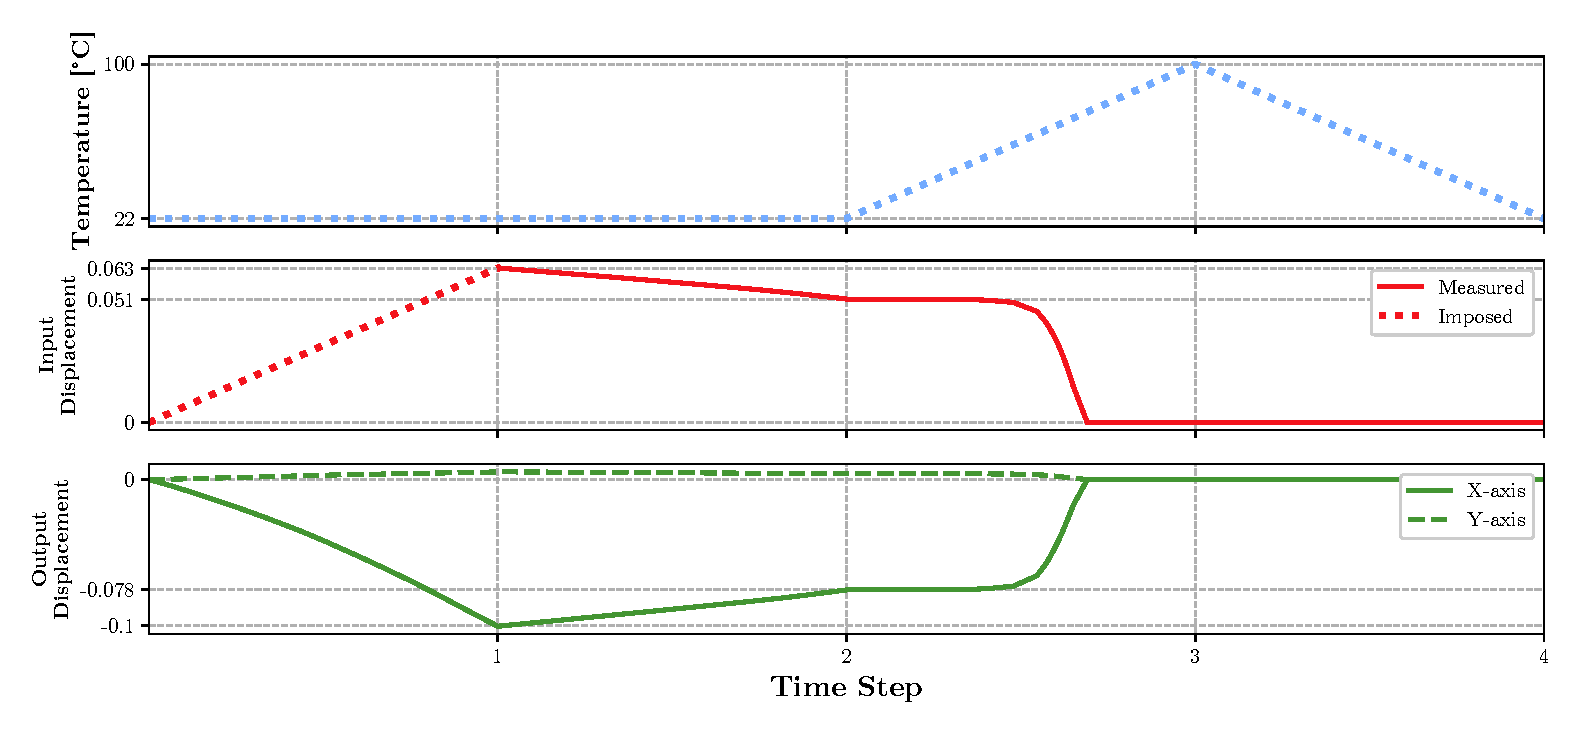
\includegraphics[width=\textwidth]{images/chap5/BM_Inverter30.eps}};
    \begin{scope}[x={(graph.south east)},y={(graph.north west)}]
    % \coordinate (ts0) at (1.54,7.6);
    % \coordinate (ts4) at (17.55,7.6);
    \coordinate (ts0) at (0.085,0.945);
    \coordinate (ts4) at (0.985,0.945);
    \coordinate (ts1) at ($ (ts0)!0.25!(ts4) $);
    \coordinate (ts2) at ($ (ts0)!0.5!(ts4) $);
    \coordinate (ts3) at ($ (ts0)!0.75!(ts4) $);
    \node[anchor=mid,inner sep=0] (ls0) at ($(ts0)!0.5!(ts1) + (0,0.05) $) {\fbox{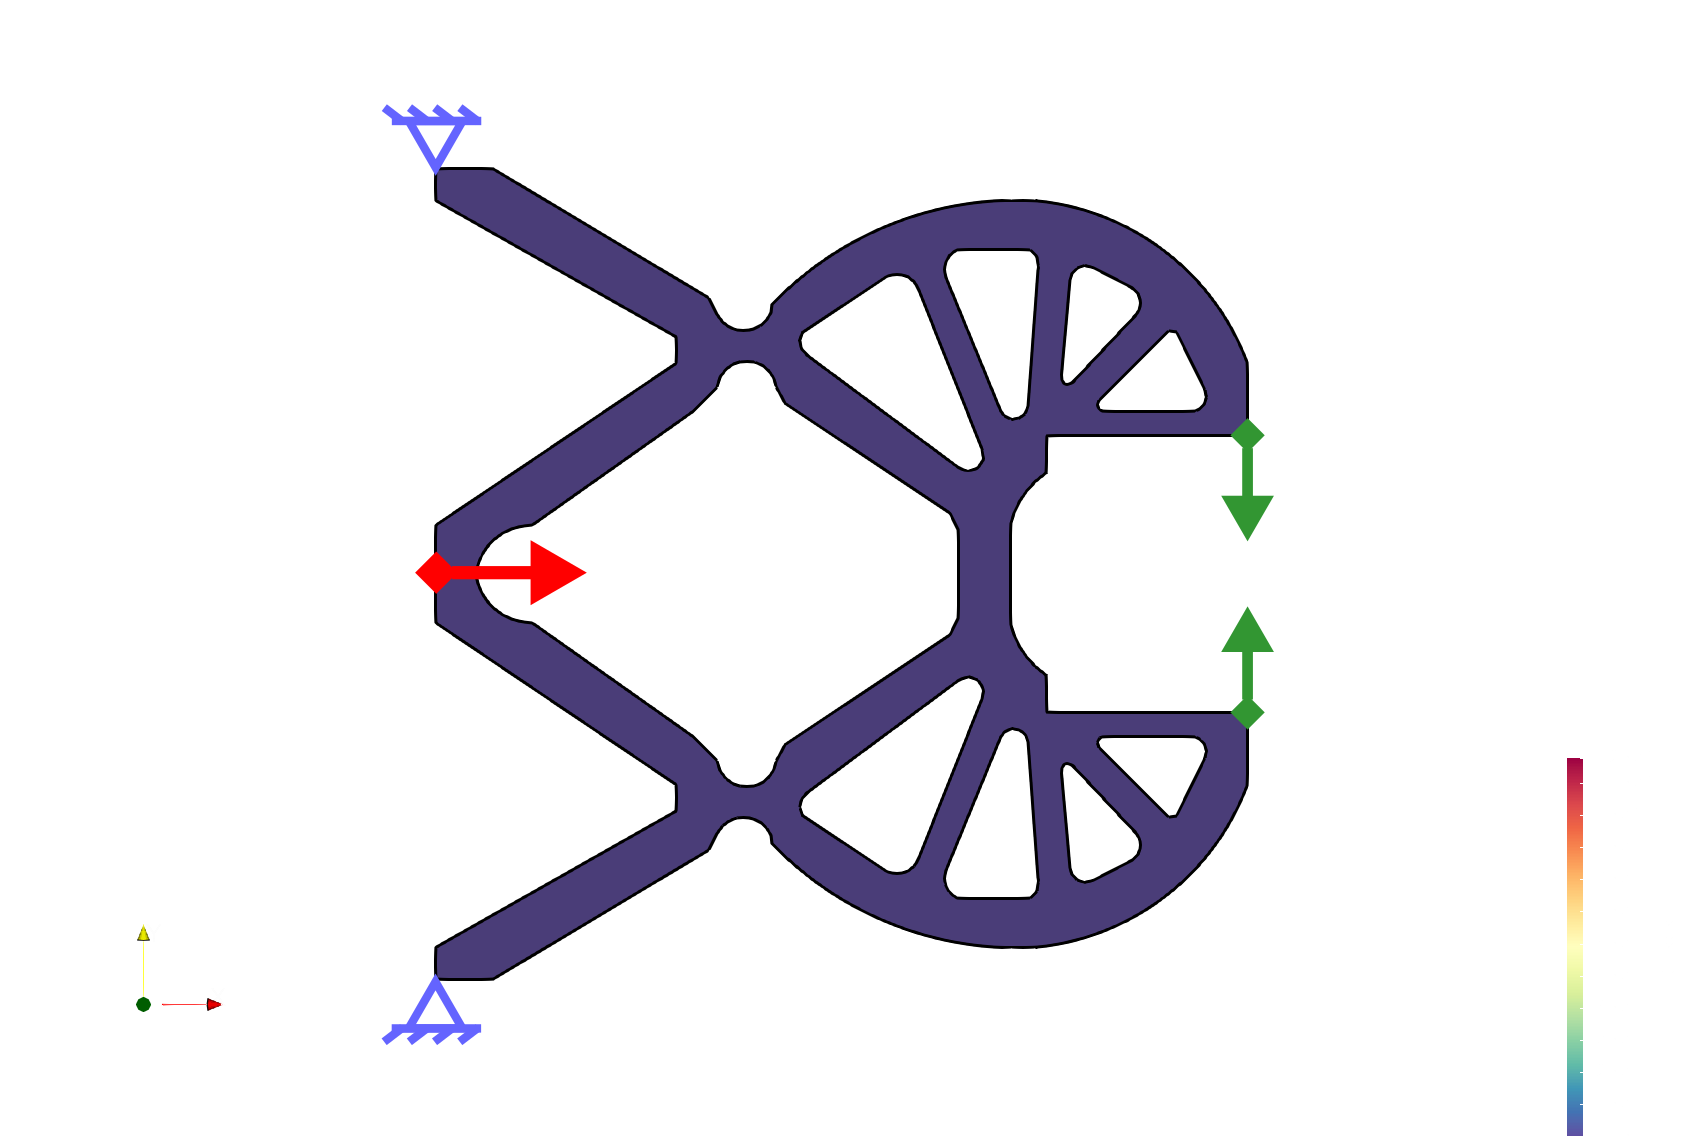
\includegraphics[height = 2cm,trim={11cm 3cm 13cm 3cm},clip]{images/chap5/Gripper_step0_v3.png}}};
    \draw[black, thick, -latex](ls0.west) to [bend right] (ts0);
    \node[anchor=mid,inner sep=0] (ls1) at ($(ts1)!0.5!(ts2) + (0,0.05) $) {\fbox{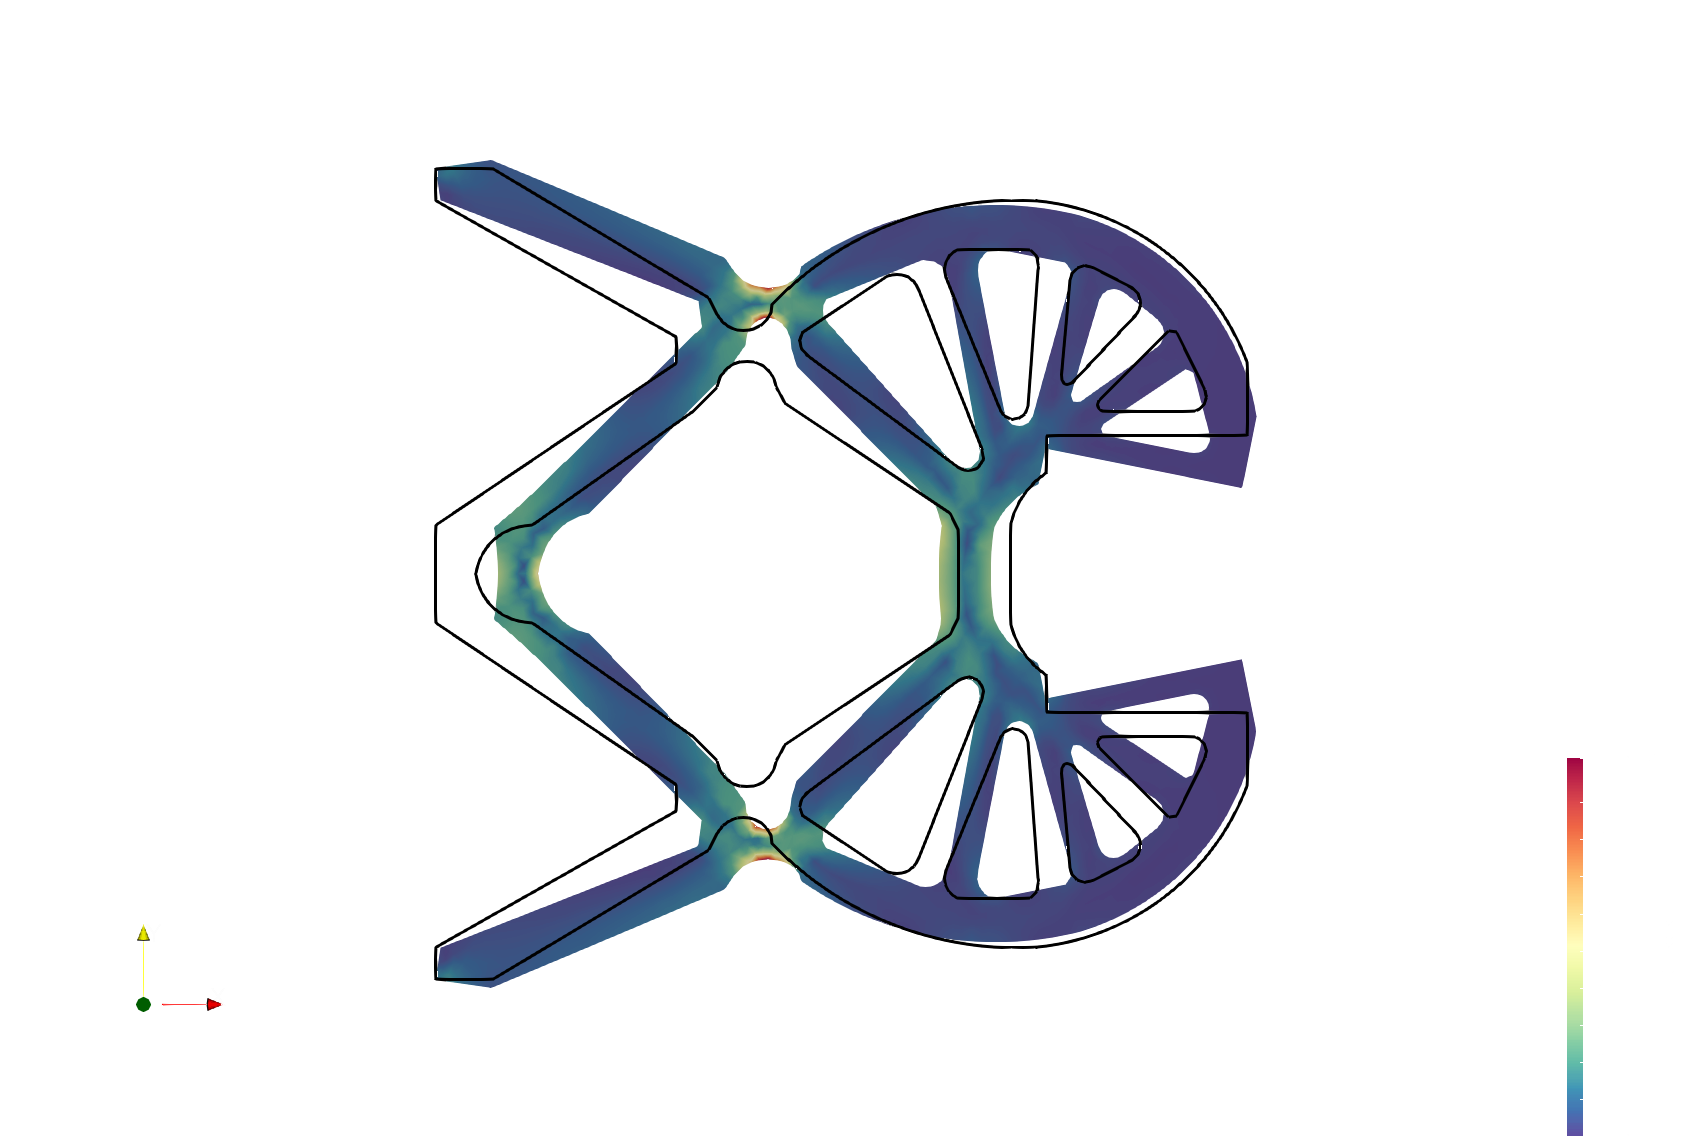
\includegraphics[height = 2cm,trim={11cm 3cm 13cm 3cm},clip]{images/chap5/Gripper_step1.png}}};
    \draw[black, thick, -latex](ls1.west) to [bend right] (ts1);
    \node[anchor=mid,inner sep=0] (ls2) at ($(ts2)!0.5!(ts3) + (0,0.05) $) {\fbox{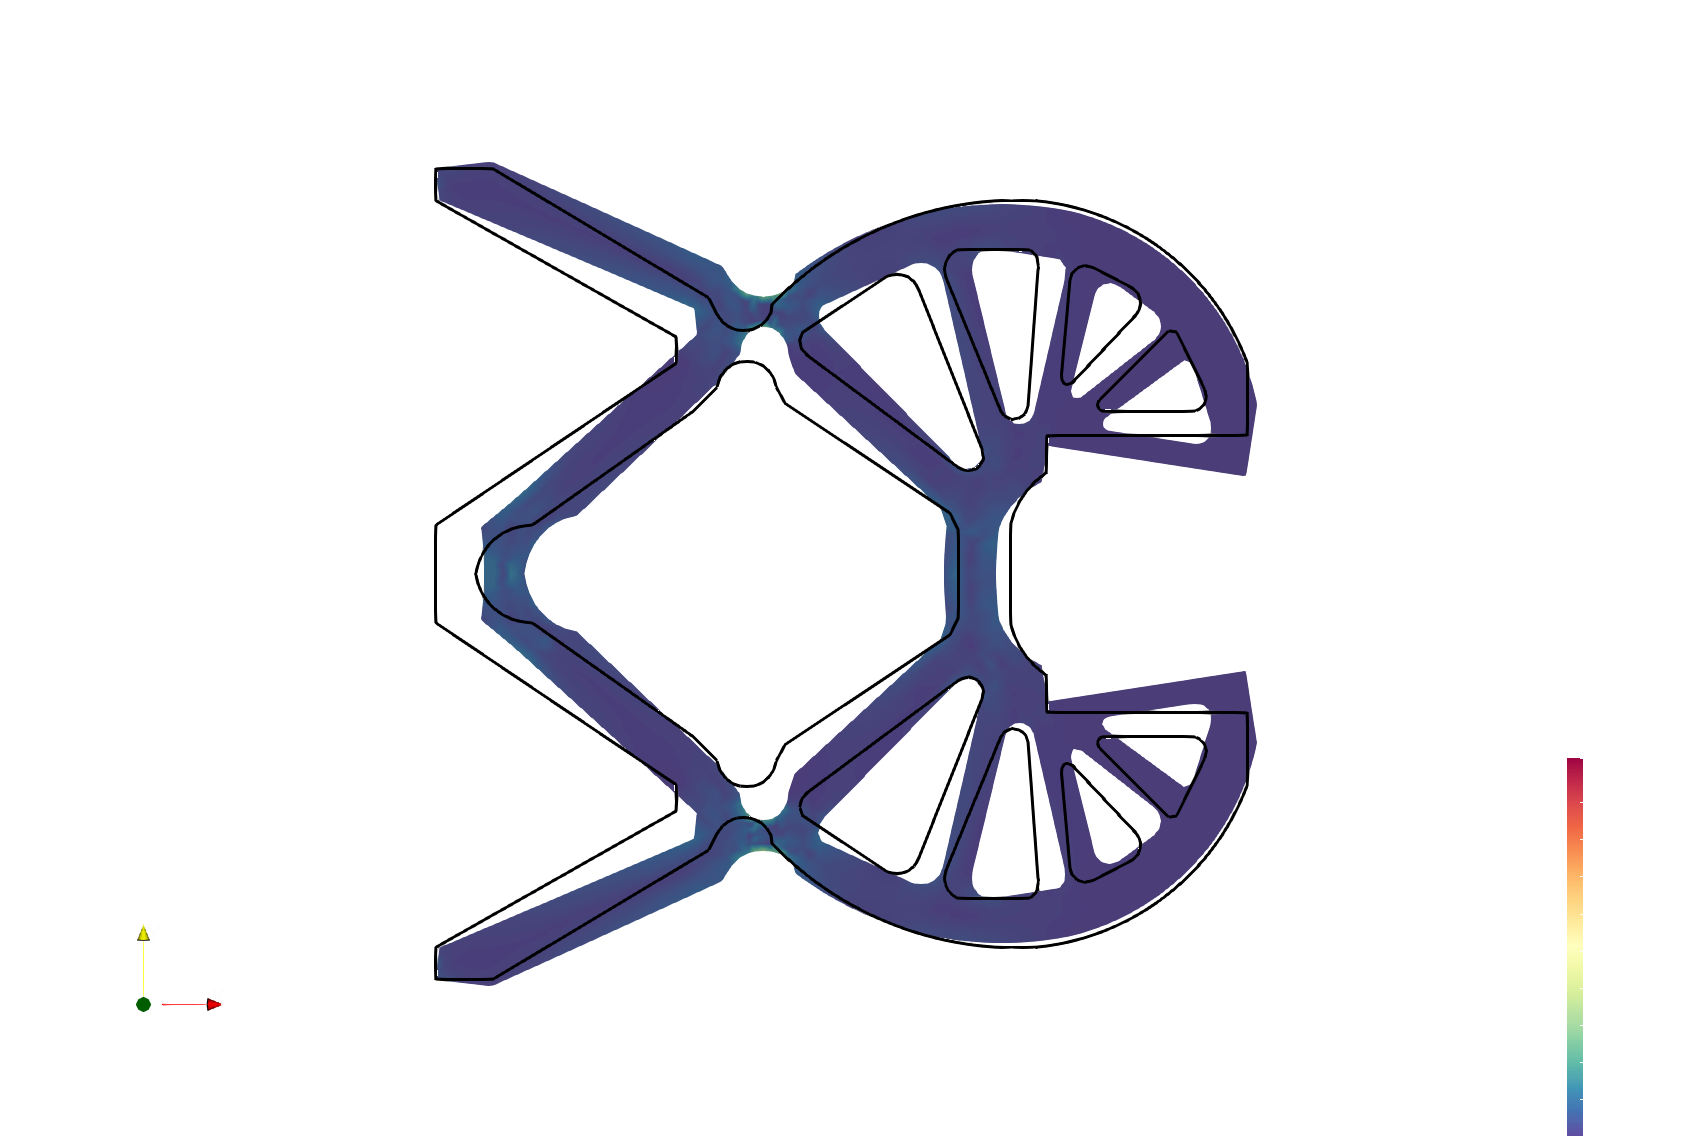
\includegraphics[height = 2cm,trim={11cm 3cm 13cm 3cm},clip]{images/chap5/Gripper_step2.png}}};
    \draw[black, thick, -latex](ls2.west) to [bend right] (ts2);
    \node[anchor=mid,inner sep=0] (ls3) at ($(ts3)!0.5!(ts4) + (0,0.05) $) {\fbox{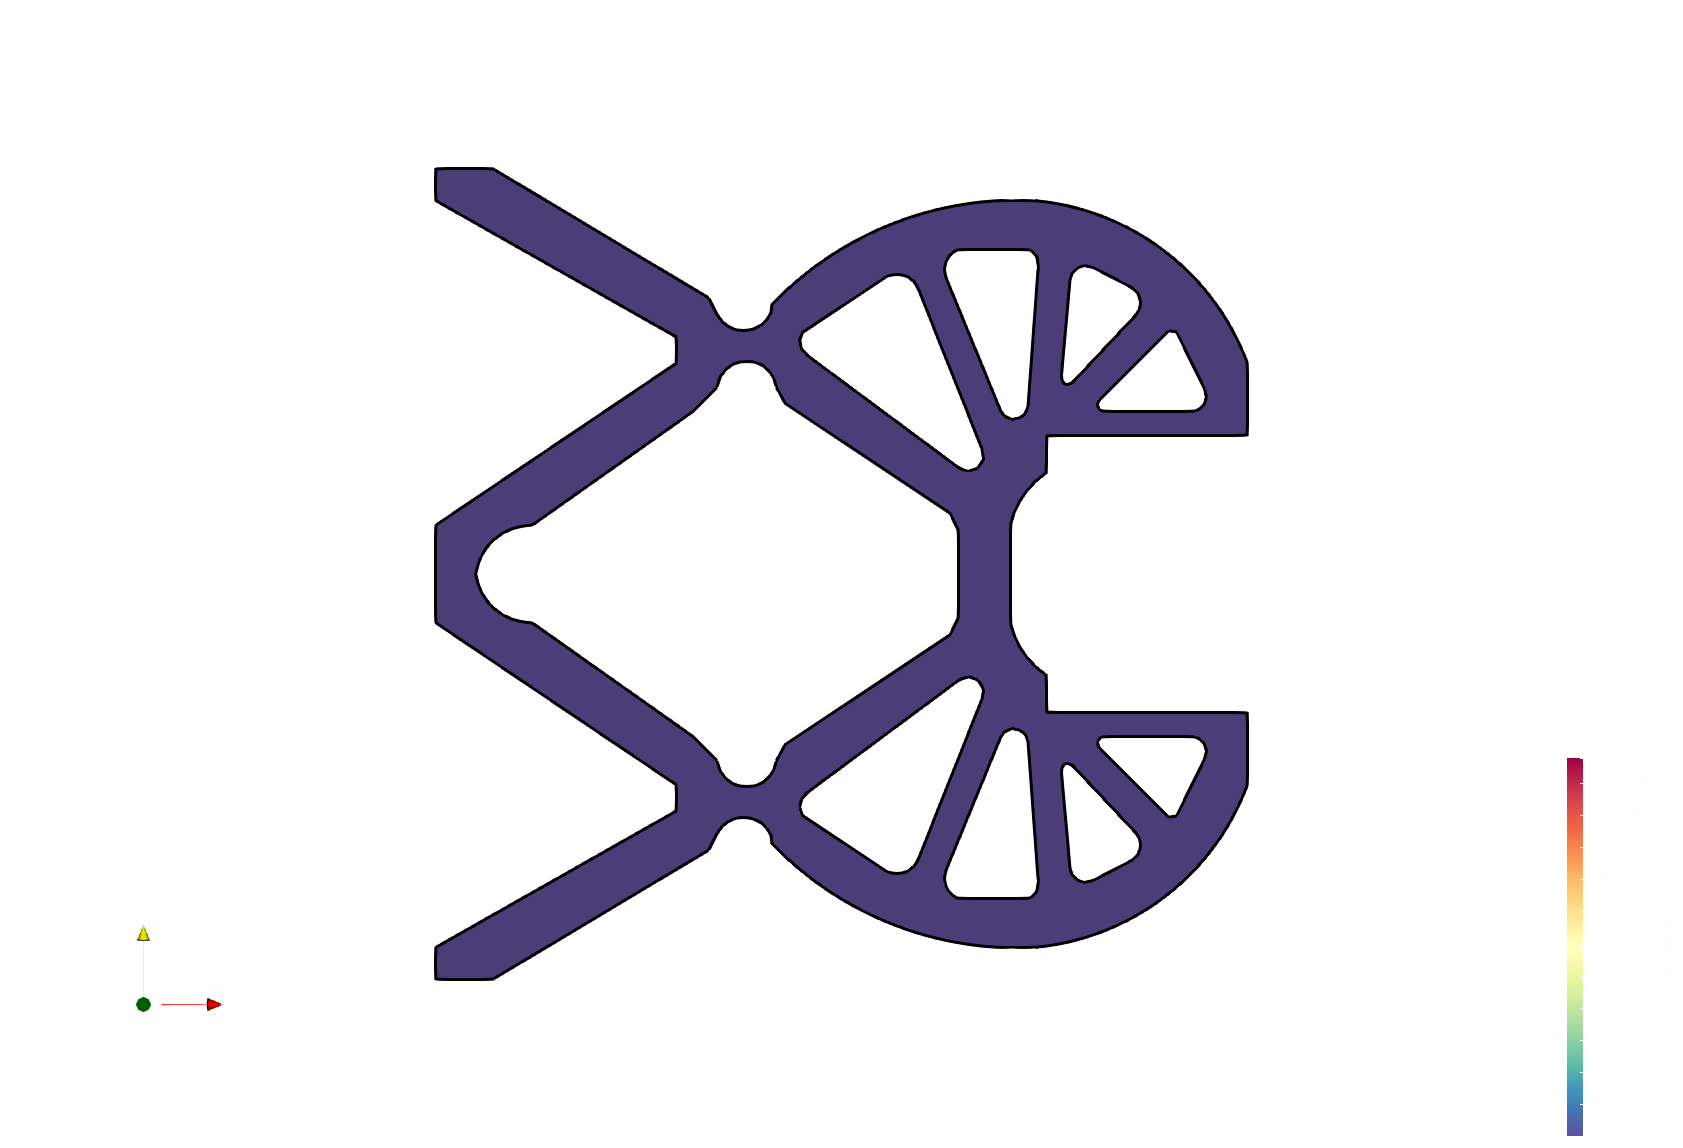
\includegraphics[height = 2cm,trim={11cm 3cm 13cm 3cm},clip]{images/chap5/Gripper_step0.png}}};
    \draw[black, thick, -latex](ls3.west) to [bend right] (ts3);
    \node[anchor=south east,inner sep=0] (ls0) at ($(ts4) + (0,0.015) $) {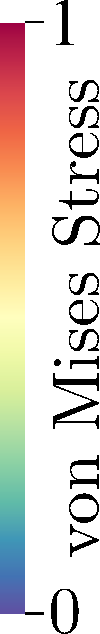
\includegraphics[height = 2.3cm]{images/chap5/Colorbar.pdf}};
    \end{scope}
    \end{tikzpicture}%
\end{document}

    \caption{Results of the shape memory effect simulation of the Inverter design showing a strain retention of $\alpha_\epsilon$ = 77.6\%.}
    \label{fig:GripperAnsysSimu}
\end{figure}

\subsection{A Qualitative Measure of the SME}
Since the topologies generated by the algorithm are widely different consisting of varying inputs, outputs and geometries, a measure by which the results can be compared is required. The final goal, being to integrate these compliant mechanisms as the active element in a biased-spring SMA actuator, the measure should represent the degree to which work has been stored by the biasing element. This measurement factor could be formulated as a measure of the relative quantity of material activate (or detwinned) by the biasing element. This implies that the larger the value of the factor is, the more optimal the biased-actuator will perform.

The amount of detwinned material in the geometry can be roughly estimated using the principle that the deformed material behaves plastically. In other words, it is the volume of the material that is able to retain its shape after the load has been released. This factor, as described in \cref{eq:strainretention}, is expressed as the strain retention factor and is defined as the amount of strain observed in the topology after the deformation load is released. This factor will vary between 0 implying non of the material has been activated and the topology retains completely back to its original shape when the load is released and 1 for a perfectly detwinned material where the entirety of the strain is retained and can only be reverted back to its original shape when heated. This strain retention factor can be calculated using :
\begin{equation}
    \StrainRetention = 1-\frac{\epsilon_\text{loaded}-\epsilon_\text{free}}{\epsilon_\text{loaded}},
    \label{eq:strainretention}
\end{equation}
with $\epsilon_\text{loaded}$ and $\epsilon_\text{free}$ representing the domain space normalised input displacement at time step 1 and 2 respectively. It is important to note that this factor can never be equal to 1 as there is some natural elastic spring back of the material even when fully detwinned and thus, is only a qualitative measure of the shape memory capabilities of the topology. It is still an effective way to compare the different topologies presented using the benchmark problems. The FEM results of the strain retention of each benchmark problem can be seen in \cref{tab:bm-fem-results}. This principle can be further extended to more complex designs where goal is to create compliant SMA structures that can have multiple outputs using just a single input biasing element which will be presented in future sections.
\begin{table}[hbt!]
    \centering
    \caption{The simulation results of the strain retention factor for each of the benchmark problems: $\boldsymbol{\mathcal{I}}$ Inverter; $\boldsymbol{\mathcal{C}}$ Crimper; $\boldsymbol{\mathcal{G}}$ Gripper}
    \label{tab:bm-fem-results}
    {\rowcolors{1}{black!5}{black!10}
     \begin{tabular}{r c c c c c c}
     \rowcolor{black} & \textbf{\color{white} $\varepsilon_\text{loaded}^x$}  & \textbf{\color{white} $\varepsilon_\text{loaded}^y$}  & \textbf{\color{white} $\varepsilon_\text{free}^x$} & \textbf{\color{white} $\varepsilon_\text{free}^y$}  & \textbf{\color{white} $\alpha_\epsilon^x$}  & \textbf{\color{white} $\alpha_\epsilon^x$} \\
     $\boldsymbol{\mathcal{I}}$ & $0.149$ & - & $0.103$ & - & \textbf{77.6\%} & - \\
     $\boldsymbol{\mathcal{C}}$ & $-0.061$ & - & $-0.048$ & - & - & \textbf{75.2\%} \\
     $\boldsymbol{\mathcal{G}}$ & $0.015$ & $-0.085$ & $0$ & $-0.065$ & \textbf{77.6\%} & - \\
 \end{tabular}}
\end{table}
\subsection{Experimental Validation of the Methodology}
In the previous section, three benchmark problems were used to validate the presence of the shape memory effect of topologically optimised compliant structures made from SMAs. Furthermore, a qualitative measure was formulated so as to compare and assess the degree to which these compliant structures would be ideal in creating biased-spring SMA actuators. However, to truly verify the presence of the shape memory effect, an experimental prototype can be fabricated.

For an accurate comparison between the FEM results and the experimental data, a prototype of a benchmark problem is conceived. For the sake of simplicity, the inverter problem is chosen due to the fact that there is only one input and output. When designing the inverter, ideal pivots are used. However when creating the experimental prototype, these ideal pivots are changed to a more realistic solution involving mounting holes. Based on these new boundary conditions, the inverter problem is redesigned using the proposed topology optimisation algorithm.

When fabricating the prototype, the cost of machining a monolithic block of NiTiNOL was deemed unfeasible. With the advent of additive manufacturing of NiTiNOL as portrayed in the work by \todocite, the creation of such compliant mechanisms has become cheaper and more feasible. However, in this case, as the topology generative is 2-Dimensional, the inverter prototype was fabricated by laser cutting thin sheets of NiTiNOL (55.8 wt. \% Ni). This laser cut inverter structure was then sandwiched between two PMMA sheets to prevent any unwanted buckling in the third dimension, as shown in \cref{fig:inverter-proto-setup}. This ensures that the deformations observed within the structure resembles the simulation.

\begin{figure}[t!]
    \centering
    \resizebox{\textwidth}{!}{% !TEX root = ../sethomas_thesis_main.tex
\documentclass[border=1mm,
               class=article
               preview]{standalone}
\usepackage{tikz}
\usepackage{tikz-imagelabels}
\imagelabelset{
   coarse grid color = red,
   fine grid color = gray,
   image label font = \sffamily\bfseries\large,
   image label distance = 2mm,
   image label back = black,
   image label text = white,
   coordinate label font = \sffamily\bfseries\large,
   coordinate label distance = 2mm,
   coordinate label back = none,
   coordinate label text = white,
   annotation font = \normalfont\small,
   arrow distance = 0mm,
   border thickness = 0.6pt,
   arrow thickness = 0.4pt,
   tip size = 1.2mm,
   outer dist = 0.1cm,
}

\begin{document}
\begin{tikzpicture}
    \node[anchor=south west,inner sep=0] (graph) at (0,0){
        \begin{annotationimage}{}{images/chap5/prototype-setup-new5.pdf}
            \draw[annotation left = {{\large PMMA plates} at 0.4}] to (0.2,0.4);
            \draw[annotation left = {{\large Pull-tester} at 0.8}] to (0.1,0.8);
            \draw[annotation right = {{\large SMA} at 0.5}] to (0.86,0.5);
            \draw[annotation right = {{\large PMMA plates} at 0.3}] to (0.94,0.3);
        \end{annotationimage}
    };
    \begin{scope}[x={(graph.south east)},y={(graph.north west)}]
        \draw [-{stealth}{stealth}{stealth}, color=white, ultra thick](0.7,0.8) --  node[below, sloped] {\Large \color{white}Input} (0.7,0.95);
        \draw [-{stealth}{stealth}{stealth}, color=white, ultra thick](0.64,0.22) --  node[below, sloped,rotate=180] {\Large \color{white}Output} (0.64,0.07);
    \end{scope}
\end{tikzpicture}%
\end{document}
}
    \caption{The experimental setup of the inverter prototype. The prototype is cut from a thin SMA sheet and is sandwiched between PMMA sheets to prevent buckling. The input load is applied using the pull-tester while measuring the input displacement and force. The output displacement is recorded using a microscopic camera.}
    \label{fig:inverter-proto-setup}
\end{figure}

The advantages of such a implementation, to test the validity of the design methodology, include the reduced cost of the prototype and more importantly, ensuring that the stress and strain distribution within the 2D structure is identical to the simulated 3D structure. This implies that the output displacement of the inverter prototype will closely resemble that of the simulated structure. The main disadvantage of this implement comes from the fact that the PMMA sheets cause lots of friction with the compliant structure. This implies that force requirements at the input will be higher than expect. As we sandwich the PMMA sheets more tightly around the compliant structure, the output displacements will be more accurate while increase the friction and force requirements to create the aforementioned output displacement. Thus, a trade-off is present but the strain retention factor, as described in \cref{eq:strainretention}, is only dependent on the the displacement and not the force requirements. Thus, the prototype was fabricated to maximise the input and output fidelity rather than the force requirement. Here, a pull-tester is used to measure the displacement of the input and the force requirements.

The goal of this section is to experimentally validate the proposed design methodology. The prototype of the compliant SMA benchmark problem was realised and must be compared to the results of the simulation. As described before, the strain retention factor was developed to compare the various generated topologies and to have a qualitative analysis of the structure to be used as a bias-spring SMA actuator. Thus, this factor can also be used to compare the experimental prototype of the modified inverter mechanism and its corresponding FEM simulation.

\begin{figure}[hbt!]
    \centering
    \resizebox{0.7\textwidth}{!}{%% Creator: Matplotlib, PGF backend
%%
%% To include the figure in your LaTeX document, write
%%   \input{<filename>.pgf}
%%
%% Make sure the required packages are loaded in your preamble
%%   \usepackage{pgf}
%%
%% Figures using additional raster images can only be included by \input if
%% they are in the same directory as the main LaTeX file. For loading figures
%% from other directories you can use the `import` package
%%   \usepackage{import}
%% and then include the figures with
%%   \import{<path to file>}{<filename>.pgf}
%%
%% Matplotlib used the following preamble
%%
\begingroup%
\makeatletter%
\begin{pgfpicture}%
\pgfpathrectangle{\pgfpointorigin}{\pgfqpoint{3.349504in}{1.562576in}}%
\pgfusepath{use as bounding box, clip}%
\begin{pgfscope}%
\pgfsetbuttcap%
\pgfsetmiterjoin%
\pgfsetlinewidth{0.000000pt}%
\definecolor{currentstroke}{rgb}{0.000000,0.000000,0.000000}%
\pgfsetstrokecolor{currentstroke}%
\pgfsetstrokeopacity{0.000000}%
\pgfsetdash{}{0pt}%
\pgfpathmoveto{\pgfqpoint{0.000000in}{0.000000in}}%
\pgfpathlineto{\pgfqpoint{3.349504in}{0.000000in}}%
\pgfpathlineto{\pgfqpoint{3.349504in}{1.562576in}}%
\pgfpathlineto{\pgfqpoint{0.000000in}{1.562576in}}%
\pgfpathclose%
\pgfusepath{}%
\end{pgfscope}%
\begin{pgfscope}%
\pgfsetbuttcap%
\pgfsetmiterjoin%
\pgfsetlinewidth{0.000000pt}%
\definecolor{currentstroke}{rgb}{0.000000,0.000000,0.000000}%
\pgfsetstrokecolor{currentstroke}%
\pgfsetstrokeopacity{0.000000}%
\pgfsetdash{}{0pt}%
\pgfpathmoveto{\pgfqpoint{0.530556in}{0.515123in}}%
\pgfpathlineto{\pgfqpoint{3.245757in}{0.515123in}}%
\pgfpathlineto{\pgfqpoint{3.245757in}{1.414351in}}%
\pgfpathlineto{\pgfqpoint{0.530556in}{1.414351in}}%
\pgfpathclose%
\pgfusepath{}%
\end{pgfscope}%
\begin{pgfscope}%
\pgfpathrectangle{\pgfqpoint{0.530556in}{0.515123in}}{\pgfqpoint{2.715201in}{0.899228in}}%
\pgfusepath{clip}%
\pgfsetbuttcap%
\pgfsetroundjoin%
\pgfsetlinewidth{0.803000pt}%
\definecolor{currentstroke}{rgb}{0.690196,0.690196,0.690196}%
\pgfsetstrokecolor{currentstroke}%
\pgfsetstrokeopacity{0.750000}%
\pgfsetdash{{0.800000pt}{1.320000pt}}{0.000000pt}%
\pgfpathmoveto{\pgfqpoint{0.653974in}{0.515123in}}%
\pgfpathlineto{\pgfqpoint{0.653974in}{1.414351in}}%
\pgfusepath{stroke}%
\end{pgfscope}%
\begin{pgfscope}%
\pgfsetbuttcap%
\pgfsetroundjoin%
\definecolor{currentfill}{rgb}{0.000000,0.000000,0.000000}%
\pgfsetfillcolor{currentfill}%
\pgfsetlinewidth{0.803000pt}%
\definecolor{currentstroke}{rgb}{0.000000,0.000000,0.000000}%
\pgfsetstrokecolor{currentstroke}%
\pgfsetdash{}{0pt}%
\pgfsys@defobject{currentmarker}{\pgfqpoint{0.000000in}{-0.048611in}}{\pgfqpoint{0.000000in}{0.000000in}}{%
\pgfpathmoveto{\pgfqpoint{0.000000in}{0.000000in}}%
\pgfpathlineto{\pgfqpoint{0.000000in}{-0.048611in}}%
\pgfusepath{stroke,fill}%
}%
\begin{pgfscope}%
\pgfsys@transformshift{0.653974in}{0.515123in}%
\pgfsys@useobject{currentmarker}{}%
\end{pgfscope}%
\end{pgfscope}%
\begin{pgfscope}%
\definecolor{textcolor}{rgb}{0.000000,0.000000,0.000000}%
\pgfsetstrokecolor{textcolor}%
\pgfsetfillcolor{textcolor}%
\pgftext[x=0.653974in,y=0.417901in,,top]{\color{textcolor}\rmfamily\fontsize{10.000000}{12.000000}\selectfont 0.00}%
\end{pgfscope}%
\begin{pgfscope}%
\pgfpathrectangle{\pgfqpoint{0.530556in}{0.515123in}}{\pgfqpoint{2.715201in}{0.899228in}}%
\pgfusepath{clip}%
\pgfsetbuttcap%
\pgfsetroundjoin%
\pgfsetlinewidth{0.803000pt}%
\definecolor{currentstroke}{rgb}{0.690196,0.690196,0.690196}%
\pgfsetstrokecolor{currentstroke}%
\pgfsetstrokeopacity{0.750000}%
\pgfsetdash{{0.800000pt}{1.320000pt}}{0.000000pt}%
\pgfpathmoveto{\pgfqpoint{1.890010in}{0.515123in}}%
\pgfpathlineto{\pgfqpoint{1.890010in}{1.414351in}}%
\pgfusepath{stroke}%
\end{pgfscope}%
\begin{pgfscope}%
\pgfsetbuttcap%
\pgfsetroundjoin%
\definecolor{currentfill}{rgb}{0.000000,0.000000,0.000000}%
\pgfsetfillcolor{currentfill}%
\pgfsetlinewidth{0.803000pt}%
\definecolor{currentstroke}{rgb}{0.000000,0.000000,0.000000}%
\pgfsetstrokecolor{currentstroke}%
\pgfsetdash{}{0pt}%
\pgfsys@defobject{currentmarker}{\pgfqpoint{0.000000in}{-0.048611in}}{\pgfqpoint{0.000000in}{0.000000in}}{%
\pgfpathmoveto{\pgfqpoint{0.000000in}{0.000000in}}%
\pgfpathlineto{\pgfqpoint{0.000000in}{-0.048611in}}%
\pgfusepath{stroke,fill}%
}%
\begin{pgfscope}%
\pgfsys@transformshift{1.890010in}{0.515123in}%
\pgfsys@useobject{currentmarker}{}%
\end{pgfscope}%
\end{pgfscope}%
\begin{pgfscope}%
\definecolor{textcolor}{rgb}{0.000000,0.000000,0.000000}%
\pgfsetstrokecolor{textcolor}%
\pgfsetfillcolor{textcolor}%
\pgftext[x=1.890010in,y=0.417901in,,top]{\color{textcolor}\rmfamily\fontsize{10.000000}{12.000000}\selectfont 1.00}%
\end{pgfscope}%
\begin{pgfscope}%
\pgfpathrectangle{\pgfqpoint{0.530556in}{0.515123in}}{\pgfqpoint{2.715201in}{0.899228in}}%
\pgfusepath{clip}%
\pgfsetbuttcap%
\pgfsetroundjoin%
\pgfsetlinewidth{0.803000pt}%
\definecolor{currentstroke}{rgb}{0.690196,0.690196,0.690196}%
\pgfsetstrokecolor{currentstroke}%
\pgfsetstrokeopacity{0.750000}%
\pgfsetdash{{0.800000pt}{1.320000pt}}{0.000000pt}%
\pgfpathmoveto{\pgfqpoint{2.735459in}{0.515123in}}%
\pgfpathlineto{\pgfqpoint{2.735459in}{1.414351in}}%
\pgfusepath{stroke}%
\end{pgfscope}%
\begin{pgfscope}%
\pgfsetbuttcap%
\pgfsetroundjoin%
\definecolor{currentfill}{rgb}{0.000000,0.000000,0.000000}%
\pgfsetfillcolor{currentfill}%
\pgfsetlinewidth{0.803000pt}%
\definecolor{currentstroke}{rgb}{0.000000,0.000000,0.000000}%
\pgfsetstrokecolor{currentstroke}%
\pgfsetdash{}{0pt}%
\pgfsys@defobject{currentmarker}{\pgfqpoint{0.000000in}{-0.048611in}}{\pgfqpoint{0.000000in}{0.000000in}}{%
\pgfpathmoveto{\pgfqpoint{0.000000in}{0.000000in}}%
\pgfpathlineto{\pgfqpoint{0.000000in}{-0.048611in}}%
\pgfusepath{stroke,fill}%
}%
\begin{pgfscope}%
\pgfsys@transformshift{2.735459in}{0.515123in}%
\pgfsys@useobject{currentmarker}{}%
\end{pgfscope}%
\end{pgfscope}%
\begin{pgfscope}%
\definecolor{textcolor}{rgb}{0.000000,0.000000,0.000000}%
\pgfsetstrokecolor{textcolor}%
\pgfsetfillcolor{textcolor}%
\pgftext[x=2.735459in,y=0.417901in,,top]{\color{textcolor}\rmfamily\fontsize{10.000000}{12.000000}\selectfont 1.68}%
\end{pgfscope}%
\begin{pgfscope}%
\pgfpathrectangle{\pgfqpoint{0.530556in}{0.515123in}}{\pgfqpoint{2.715201in}{0.899228in}}%
\pgfusepath{clip}%
\pgfsetbuttcap%
\pgfsetroundjoin%
\pgfsetlinewidth{0.803000pt}%
\definecolor{currentstroke}{rgb}{0.690196,0.690196,0.690196}%
\pgfsetstrokecolor{currentstroke}%
\pgfsetstrokeopacity{0.750000}%
\pgfsetdash{{0.800000pt}{1.320000pt}}{0.000000pt}%
\pgfpathmoveto{\pgfqpoint{3.126047in}{0.515123in}}%
\pgfpathlineto{\pgfqpoint{3.126047in}{1.414351in}}%
\pgfusepath{stroke}%
\end{pgfscope}%
\begin{pgfscope}%
\pgfsetbuttcap%
\pgfsetroundjoin%
\definecolor{currentfill}{rgb}{0.000000,0.000000,0.000000}%
\pgfsetfillcolor{currentfill}%
\pgfsetlinewidth{0.803000pt}%
\definecolor{currentstroke}{rgb}{0.000000,0.000000,0.000000}%
\pgfsetstrokecolor{currentstroke}%
\pgfsetdash{}{0pt}%
\pgfsys@defobject{currentmarker}{\pgfqpoint{0.000000in}{-0.048611in}}{\pgfqpoint{0.000000in}{0.000000in}}{%
\pgfpathmoveto{\pgfqpoint{0.000000in}{0.000000in}}%
\pgfpathlineto{\pgfqpoint{0.000000in}{-0.048611in}}%
\pgfusepath{stroke,fill}%
}%
\begin{pgfscope}%
\pgfsys@transformshift{3.126047in}{0.515123in}%
\pgfsys@useobject{currentmarker}{}%
\end{pgfscope}%
\end{pgfscope}%
\begin{pgfscope}%
\definecolor{textcolor}{rgb}{0.000000,0.000000,0.000000}%
\pgfsetstrokecolor{textcolor}%
\pgfsetfillcolor{textcolor}%
\pgftext[x=3.126047in,y=0.417901in,,top]{\color{textcolor}\rmfamily\fontsize{10.000000}{12.000000}\selectfont 2.00}%
\end{pgfscope}%
\begin{pgfscope}%
\definecolor{textcolor}{rgb}{0.000000,0.000000,0.000000}%
\pgfsetstrokecolor{textcolor}%
\pgfsetfillcolor{textcolor}%
\pgftext[x=1.888156in,y=0.238889in,,top]{\color{textcolor}\rmfamily\fontsize{10.000000}{12.000000}\selectfont Displacement [mm]}%
\end{pgfscope}%
\begin{pgfscope}%
\pgfpathrectangle{\pgfqpoint{0.530556in}{0.515123in}}{\pgfqpoint{2.715201in}{0.899228in}}%
\pgfusepath{clip}%
\pgfsetbuttcap%
\pgfsetroundjoin%
\pgfsetlinewidth{0.803000pt}%
\definecolor{currentstroke}{rgb}{0.690196,0.690196,0.690196}%
\pgfsetstrokecolor{currentstroke}%
\pgfsetstrokeopacity{0.750000}%
\pgfsetdash{{0.800000pt}{1.320000pt}}{0.000000pt}%
\pgfpathmoveto{\pgfqpoint{0.530556in}{0.528958in}}%
\pgfpathlineto{\pgfqpoint{3.245757in}{0.528958in}}%
\pgfusepath{stroke}%
\end{pgfscope}%
\begin{pgfscope}%
\pgfsetbuttcap%
\pgfsetroundjoin%
\definecolor{currentfill}{rgb}{0.000000,0.000000,0.000000}%
\pgfsetfillcolor{currentfill}%
\pgfsetlinewidth{0.803000pt}%
\definecolor{currentstroke}{rgb}{0.000000,0.000000,0.000000}%
\pgfsetstrokecolor{currentstroke}%
\pgfsetdash{}{0pt}%
\pgfsys@defobject{currentmarker}{\pgfqpoint{-0.048611in}{0.000000in}}{\pgfqpoint{0.000000in}{0.000000in}}{%
\pgfpathmoveto{\pgfqpoint{0.000000in}{0.000000in}}%
\pgfpathlineto{\pgfqpoint{-0.048611in}{0.000000in}}%
\pgfusepath{stroke,fill}%
}%
\begin{pgfscope}%
\pgfsys@transformshift{0.530556in}{0.528958in}%
\pgfsys@useobject{currentmarker}{}%
\end{pgfscope}%
\end{pgfscope}%
\begin{pgfscope}%
\definecolor{textcolor}{rgb}{0.000000,0.000000,0.000000}%
\pgfsetstrokecolor{textcolor}%
\pgfsetfillcolor{textcolor}%
\pgftext[x=0.363889in,y=0.480732in,left,base]{\color{textcolor}\rmfamily\fontsize{10.000000}{12.000000}\selectfont \(\displaystyle 0\)}%
\end{pgfscope}%
\begin{pgfscope}%
\pgfpathrectangle{\pgfqpoint{0.530556in}{0.515123in}}{\pgfqpoint{2.715201in}{0.899228in}}%
\pgfusepath{clip}%
\pgfsetbuttcap%
\pgfsetroundjoin%
\pgfsetlinewidth{0.803000pt}%
\definecolor{currentstroke}{rgb}{0.690196,0.690196,0.690196}%
\pgfsetstrokecolor{currentstroke}%
\pgfsetstrokeopacity{0.750000}%
\pgfsetdash{{0.800000pt}{1.320000pt}}{0.000000pt}%
\pgfpathmoveto{\pgfqpoint{0.530556in}{0.750306in}}%
\pgfpathlineto{\pgfqpoint{3.245757in}{0.750306in}}%
\pgfusepath{stroke}%
\end{pgfscope}%
\begin{pgfscope}%
\pgfsetbuttcap%
\pgfsetroundjoin%
\definecolor{currentfill}{rgb}{0.000000,0.000000,0.000000}%
\pgfsetfillcolor{currentfill}%
\pgfsetlinewidth{0.803000pt}%
\definecolor{currentstroke}{rgb}{0.000000,0.000000,0.000000}%
\pgfsetstrokecolor{currentstroke}%
\pgfsetdash{}{0pt}%
\pgfsys@defobject{currentmarker}{\pgfqpoint{-0.048611in}{0.000000in}}{\pgfqpoint{0.000000in}{0.000000in}}{%
\pgfpathmoveto{\pgfqpoint{0.000000in}{0.000000in}}%
\pgfpathlineto{\pgfqpoint{-0.048611in}{0.000000in}}%
\pgfusepath{stroke,fill}%
}%
\begin{pgfscope}%
\pgfsys@transformshift{0.530556in}{0.750306in}%
\pgfsys@useobject{currentmarker}{}%
\end{pgfscope}%
\end{pgfscope}%
\begin{pgfscope}%
\definecolor{textcolor}{rgb}{0.000000,0.000000,0.000000}%
\pgfsetstrokecolor{textcolor}%
\pgfsetfillcolor{textcolor}%
\pgftext[x=0.363889in,y=0.702081in,left,base]{\color{textcolor}\rmfamily\fontsize{10.000000}{12.000000}\selectfont \(\displaystyle 4\)}%
\end{pgfscope}%
\begin{pgfscope}%
\pgfpathrectangle{\pgfqpoint{0.530556in}{0.515123in}}{\pgfqpoint{2.715201in}{0.899228in}}%
\pgfusepath{clip}%
\pgfsetbuttcap%
\pgfsetroundjoin%
\pgfsetlinewidth{0.803000pt}%
\definecolor{currentstroke}{rgb}{0.690196,0.690196,0.690196}%
\pgfsetstrokecolor{currentstroke}%
\pgfsetstrokeopacity{0.750000}%
\pgfsetdash{{0.800000pt}{1.320000pt}}{0.000000pt}%
\pgfpathmoveto{\pgfqpoint{0.530556in}{0.971654in}}%
\pgfpathlineto{\pgfqpoint{3.245757in}{0.971654in}}%
\pgfusepath{stroke}%
\end{pgfscope}%
\begin{pgfscope}%
\pgfsetbuttcap%
\pgfsetroundjoin%
\definecolor{currentfill}{rgb}{0.000000,0.000000,0.000000}%
\pgfsetfillcolor{currentfill}%
\pgfsetlinewidth{0.803000pt}%
\definecolor{currentstroke}{rgb}{0.000000,0.000000,0.000000}%
\pgfsetstrokecolor{currentstroke}%
\pgfsetdash{}{0pt}%
\pgfsys@defobject{currentmarker}{\pgfqpoint{-0.048611in}{0.000000in}}{\pgfqpoint{0.000000in}{0.000000in}}{%
\pgfpathmoveto{\pgfqpoint{0.000000in}{0.000000in}}%
\pgfpathlineto{\pgfqpoint{-0.048611in}{0.000000in}}%
\pgfusepath{stroke,fill}%
}%
\begin{pgfscope}%
\pgfsys@transformshift{0.530556in}{0.971654in}%
\pgfsys@useobject{currentmarker}{}%
\end{pgfscope}%
\end{pgfscope}%
\begin{pgfscope}%
\definecolor{textcolor}{rgb}{0.000000,0.000000,0.000000}%
\pgfsetstrokecolor{textcolor}%
\pgfsetfillcolor{textcolor}%
\pgftext[x=0.363889in,y=0.923429in,left,base]{\color{textcolor}\rmfamily\fontsize{10.000000}{12.000000}\selectfont \(\displaystyle 8\)}%
\end{pgfscope}%
\begin{pgfscope}%
\pgfpathrectangle{\pgfqpoint{0.530556in}{0.515123in}}{\pgfqpoint{2.715201in}{0.899228in}}%
\pgfusepath{clip}%
\pgfsetbuttcap%
\pgfsetroundjoin%
\pgfsetlinewidth{0.803000pt}%
\definecolor{currentstroke}{rgb}{0.690196,0.690196,0.690196}%
\pgfsetstrokecolor{currentstroke}%
\pgfsetstrokeopacity{0.750000}%
\pgfsetdash{{0.800000pt}{1.320000pt}}{0.000000pt}%
\pgfpathmoveto{\pgfqpoint{0.530556in}{1.193003in}}%
\pgfpathlineto{\pgfqpoint{3.245757in}{1.193003in}}%
\pgfusepath{stroke}%
\end{pgfscope}%
\begin{pgfscope}%
\pgfsetbuttcap%
\pgfsetroundjoin%
\definecolor{currentfill}{rgb}{0.000000,0.000000,0.000000}%
\pgfsetfillcolor{currentfill}%
\pgfsetlinewidth{0.803000pt}%
\definecolor{currentstroke}{rgb}{0.000000,0.000000,0.000000}%
\pgfsetstrokecolor{currentstroke}%
\pgfsetdash{}{0pt}%
\pgfsys@defobject{currentmarker}{\pgfqpoint{-0.048611in}{0.000000in}}{\pgfqpoint{0.000000in}{0.000000in}}{%
\pgfpathmoveto{\pgfqpoint{0.000000in}{0.000000in}}%
\pgfpathlineto{\pgfqpoint{-0.048611in}{0.000000in}}%
\pgfusepath{stroke,fill}%
}%
\begin{pgfscope}%
\pgfsys@transformshift{0.530556in}{1.193003in}%
\pgfsys@useobject{currentmarker}{}%
\end{pgfscope}%
\end{pgfscope}%
\begin{pgfscope}%
\definecolor{textcolor}{rgb}{0.000000,0.000000,0.000000}%
\pgfsetstrokecolor{textcolor}%
\pgfsetfillcolor{textcolor}%
\pgftext[x=0.294444in,y=1.144777in,left,base]{\color{textcolor}\rmfamily\fontsize{10.000000}{12.000000}\selectfont \(\displaystyle 12\)}%
\end{pgfscope}%
\begin{pgfscope}%
\pgfpathrectangle{\pgfqpoint{0.530556in}{0.515123in}}{\pgfqpoint{2.715201in}{0.899228in}}%
\pgfusepath{clip}%
\pgfsetbuttcap%
\pgfsetroundjoin%
\pgfsetlinewidth{0.803000pt}%
\definecolor{currentstroke}{rgb}{0.690196,0.690196,0.690196}%
\pgfsetstrokecolor{currentstroke}%
\pgfsetstrokeopacity{0.750000}%
\pgfsetdash{{0.800000pt}{1.320000pt}}{0.000000pt}%
\pgfpathmoveto{\pgfqpoint{0.530556in}{1.414351in}}%
\pgfpathlineto{\pgfqpoint{3.245757in}{1.414351in}}%
\pgfusepath{stroke}%
\end{pgfscope}%
\begin{pgfscope}%
\pgfsetbuttcap%
\pgfsetroundjoin%
\definecolor{currentfill}{rgb}{0.000000,0.000000,0.000000}%
\pgfsetfillcolor{currentfill}%
\pgfsetlinewidth{0.803000pt}%
\definecolor{currentstroke}{rgb}{0.000000,0.000000,0.000000}%
\pgfsetstrokecolor{currentstroke}%
\pgfsetdash{}{0pt}%
\pgfsys@defobject{currentmarker}{\pgfqpoint{-0.048611in}{0.000000in}}{\pgfqpoint{0.000000in}{0.000000in}}{%
\pgfpathmoveto{\pgfqpoint{0.000000in}{0.000000in}}%
\pgfpathlineto{\pgfqpoint{-0.048611in}{0.000000in}}%
\pgfusepath{stroke,fill}%
}%
\begin{pgfscope}%
\pgfsys@transformshift{0.530556in}{1.414351in}%
\pgfsys@useobject{currentmarker}{}%
\end{pgfscope}%
\end{pgfscope}%
\begin{pgfscope}%
\definecolor{textcolor}{rgb}{0.000000,0.000000,0.000000}%
\pgfsetstrokecolor{textcolor}%
\pgfsetfillcolor{textcolor}%
\pgftext[x=0.294444in,y=1.366126in,left,base]{\color{textcolor}\rmfamily\fontsize{10.000000}{12.000000}\selectfont \(\displaystyle 16\)}%
\end{pgfscope}%
\begin{pgfscope}%
\definecolor{textcolor}{rgb}{0.000000,0.000000,0.000000}%
\pgfsetstrokecolor{textcolor}%
\pgfsetfillcolor{textcolor}%
\pgftext[x=0.238889in,y=0.964737in,,bottom,rotate=90.000000]{\color{textcolor}\rmfamily\fontsize{10.000000}{12.000000}\selectfont Force [N]}%
\end{pgfscope}%
\begin{pgfscope}%
\pgfpathrectangle{\pgfqpoint{0.530556in}{0.515123in}}{\pgfqpoint{2.715201in}{0.899228in}}%
\pgfusepath{clip}%
\pgfsetbuttcap%
\pgfsetroundjoin%
\pgfsetlinewidth{2.007500pt}%
\definecolor{currentstroke}{rgb}{0.317647,0.596078,0.423529}%
\pgfsetstrokecolor{currentstroke}%
\pgfsetdash{{2.000000pt}{3.300000pt}}{0.000000pt}%
\pgfpathmoveto{\pgfqpoint{0.653974in}{0.528958in}}%
\pgfpathlineto{\pgfqpoint{0.653974in}{0.528958in}}%
\pgfpathlineto{\pgfqpoint{0.653974in}{0.528958in}}%
\pgfpathlineto{\pgfqpoint{0.653974in}{0.528958in}}%
\pgfpathlineto{\pgfqpoint{0.653974in}{0.528958in}}%
\pgfpathlineto{\pgfqpoint{0.653974in}{0.528958in}}%
\pgfpathlineto{\pgfqpoint{0.653974in}{0.528958in}}%
\pgfpathlineto{\pgfqpoint{0.664688in}{0.533431in}}%
\pgfpathlineto{\pgfqpoint{0.737655in}{0.561127in}}%
\pgfpathlineto{\pgfqpoint{0.821009in}{0.571374in}}%
\pgfpathlineto{\pgfqpoint{0.905149in}{0.589021in}}%
\pgfpathlineto{\pgfqpoint{0.988274in}{0.607654in}}%
\pgfpathlineto{\pgfqpoint{1.071939in}{0.610944in}}%
\pgfpathlineto{\pgfqpoint{1.156864in}{0.620500in}}%
\pgfpathlineto{\pgfqpoint{1.239492in}{0.630774in}}%
\pgfpathlineto{\pgfqpoint{1.322659in}{0.640685in}}%
\pgfpathlineto{\pgfqpoint{1.406708in}{0.646520in}}%
\pgfpathlineto{\pgfqpoint{1.489373in}{0.650898in}}%
\pgfpathlineto{\pgfqpoint{1.572829in}{0.676384in}}%
\pgfpathlineto{\pgfqpoint{1.656430in}{0.735182in}}%
\pgfpathlineto{\pgfqpoint{1.738967in}{0.781032in}}%
\pgfpathlineto{\pgfqpoint{1.821900in}{0.818988in}}%
\pgfpathlineto{\pgfqpoint{1.905009in}{0.875454in}}%
\pgfpathlineto{\pgfqpoint{1.986864in}{0.930572in}}%
\pgfpathlineto{\pgfqpoint{2.069703in}{0.973501in}}%
\pgfpathlineto{\pgfqpoint{2.153205in}{1.010356in}}%
\pgfpathlineto{\pgfqpoint{2.235677in}{1.048709in}}%
\pgfpathlineto{\pgfqpoint{2.318797in}{1.081891in}}%
\pgfpathlineto{\pgfqpoint{2.402383in}{1.102959in}}%
\pgfpathlineto{\pgfqpoint{2.484454in}{1.126167in}}%
\pgfpathlineto{\pgfqpoint{2.567204in}{1.167154in}}%
\pgfpathlineto{\pgfqpoint{2.650744in}{1.208680in}}%
\pgfpathlineto{\pgfqpoint{2.733015in}{1.246137in}}%
\pgfpathlineto{\pgfqpoint{2.816303in}{1.266993in}}%
\pgfpathlineto{\pgfqpoint{2.900231in}{1.292055in}}%
\pgfpathlineto{\pgfqpoint{2.982839in}{1.322953in}}%
\pgfpathlineto{\pgfqpoint{3.066168in}{1.356134in}}%
\pgfpathlineto{\pgfqpoint{3.121133in}{1.333083in}}%
\pgfpathlineto{\pgfqpoint{3.122339in}{1.293102in}}%
\pgfpathlineto{\pgfqpoint{3.122339in}{1.278136in}}%
\pgfpathlineto{\pgfqpoint{3.122339in}{1.265208in}}%
\pgfpathlineto{\pgfqpoint{3.122339in}{1.257465in}}%
\pgfpathlineto{\pgfqpoint{3.115164in}{1.153364in}}%
\pgfpathlineto{\pgfqpoint{3.078533in}{0.868374in}}%
\pgfpathlineto{\pgfqpoint{3.037500in}{0.724265in}}%
\pgfpathlineto{\pgfqpoint{2.996882in}{0.627791in}}%
\pgfpathlineto{\pgfqpoint{2.956148in}{0.567605in}}%
\pgfpathlineto{\pgfqpoint{2.915147in}{0.531153in}}%
\pgfpathlineto{\pgfqpoint{2.873385in}{0.522247in}}%
\pgfpathlineto{\pgfqpoint{2.831325in}{0.519190in}}%
\pgfpathlineto{\pgfqpoint{2.789338in}{0.517890in}}%
\pgfpathlineto{\pgfqpoint{2.747771in}{0.519354in}}%
\pgfpathlineto{\pgfqpoint{2.727686in}{0.511790in}}%
\pgfusepath{stroke}%
\end{pgfscope}%
\begin{pgfscope}%
\pgfsetrectcap%
\pgfsetmiterjoin%
\pgfsetlinewidth{0.803000pt}%
\definecolor{currentstroke}{rgb}{0.000000,0.000000,0.000000}%
\pgfsetstrokecolor{currentstroke}%
\pgfsetdash{}{0pt}%
\pgfpathmoveto{\pgfqpoint{0.530556in}{0.515123in}}%
\pgfpathlineto{\pgfqpoint{0.530556in}{1.414351in}}%
\pgfusepath{stroke}%
\end{pgfscope}%
\begin{pgfscope}%
\pgfsetrectcap%
\pgfsetmiterjoin%
\pgfsetlinewidth{0.803000pt}%
\definecolor{currentstroke}{rgb}{0.000000,0.000000,0.000000}%
\pgfsetstrokecolor{currentstroke}%
\pgfsetdash{}{0pt}%
\pgfpathmoveto{\pgfqpoint{3.245757in}{0.515123in}}%
\pgfpathlineto{\pgfqpoint{3.245757in}{1.414351in}}%
\pgfusepath{stroke}%
\end{pgfscope}%
\begin{pgfscope}%
\pgfsetrectcap%
\pgfsetmiterjoin%
\pgfsetlinewidth{0.803000pt}%
\definecolor{currentstroke}{rgb}{0.000000,0.000000,0.000000}%
\pgfsetstrokecolor{currentstroke}%
\pgfsetdash{}{0pt}%
\pgfpathmoveto{\pgfqpoint{0.530556in}{0.515123in}}%
\pgfpathlineto{\pgfqpoint{3.245757in}{0.515123in}}%
\pgfusepath{stroke}%
\end{pgfscope}%
\begin{pgfscope}%
\pgfsetrectcap%
\pgfsetmiterjoin%
\pgfsetlinewidth{0.803000pt}%
\definecolor{currentstroke}{rgb}{0.000000,0.000000,0.000000}%
\pgfsetstrokecolor{currentstroke}%
\pgfsetdash{}{0pt}%
\pgfpathmoveto{\pgfqpoint{0.530556in}{1.414351in}}%
\pgfpathlineto{\pgfqpoint{3.245757in}{1.414351in}}%
\pgfusepath{stroke}%
\end{pgfscope}%
\end{pgfpicture}%
\makeatother%
\endgroup%
}
    \caption{The experimental results of the inverter prototype are obtained using a pull-tester and a strain retention of 84.3\% is observed.}
    \label{fig:results-proto-inverter}
\end{figure}%

In \cref{fig:results-proto-inverter}, the pull-tester results can be seen. The strain retention is measured by applying an initial strain to the input of the prototype using the pull-tester. By then reversing the direction of the pull-tester and measuring the reaction force, the point at which the reaction force descends below $0$ N will define the strain that is retained by the structure after the initial load is released. We assume that as the pull-tester observes a value below $-0.2$ N, the structure has overcome the internal friction with the PMMA sheets and is now bending the input of the prototype rather than returning to its original shape. Based on the values observed using the pull-tester, a strain retention of $84.2$\% is measured as shown in \cref{tab:inverter-prototype-fem-results}. When comparing to the results of the simulation of the same modified inverter topology of $78.9$\%, the shape memory effect capabilities of topologies generated by this design approach is validated. The difference in the strain retention between the experimental and FEM results can be accounted by the friction present in the physical implementation.

\begin{table}[hbt!]
    \centering
    \caption{Comparison between the FEM and experimental results of the modified inverter benchmark problem.}
    \label{tab:inverter-prototype-fem-results}
    {\rowcolors{1}{black!5}{black!10}
     \begin{tabular}{r c c c}
     \rowcolor{black} & \textbf{\color{white} $x_\text{loaded}$ [mm]}  & \textbf{\color{white} $x_\text{free}$ [mm]} & \textbf{\color{white} $\alpha_\epsilon$ [\%]}\\
     FEM & 2.0 & 1.58 & 78.9 \\
     Expt. & 2.0 & 1.68 & 84.3 \\
 \end{tabular}}
\end{table}

\section{Proposed Induction Heating Strategy}
Due to the complex geometries of the generated topologies, simply passing a current through the structure by attaching electrode to the ends is no longer possible. In the case of inverter prototype, electrodes must be attached at multiple points so as to allow current to flow through all the areas of the geometry.

Various works have been established where surface mounted coils have been installed to function as a heating coil that raise the temperature of the SMA structures for localised heating, as shown in the work by \todocite. This can be quite cumbersome due to possible risks of delamination while the SMA contracts and dilates during actuation. Another option would be to use hot air as a medium to increase the temperature of the SMA structure, perhaps with tools such as hot air guns. These external heating structure drastically reduce the work density of the resulting actuator and are thus, rarely used in small and compact applications.

Due to the complex geometry of the inverter prototype, the current paths for Joule's heating are no longer unique, nor trivial anymore. Here, in this case, multiple electrodes with multiple external wires are required to heat the structure. Thus, here, the proposed heating solution consists of a contactless, wireless strategy where a current is induced within the SMA structures using external induction coils.
\subsection{Magnetic Induction Heating}
The basic working principle of the proposed heating methodology and its application in the inverter mechanism can be seen in \todocite. By passing an alternating current at a high frequency is passed through the primary coil and generates a magnetic field. When any electric conductor, the SMA structure in this case, is placed inside the generated magnetic field, a secondary electric current, $\InducedCurrent$, is induced inside the structure. This induced current will generate Joule's losses, $\PJoules$, heating the SMA :
\begin{equation}
    \PJoules = \ResisSMA \cdot \InducedCurrent^2 = \frac{\VoltageEMF^2}{\ResisSMA}.
\end{equation}
The magnitude of the current is based on the electromotive force, $\VoltageEMF$, generated by the primary coil, and the effective resistance, $\ResisSMA$, of the path taken by the induced current. The coupling between the primary coil and the SMA piece, as described in \cref{eq:back_emf}, dictates the electromotive force.
\begin{equation}
    \label{eq:back_emf}
    \VoltageEMF^2 = \Big(-\frac{\text{d}\TotalFlux}{\text{dt}}\Big)^2 = \Big(- 2\pi \frequency \Inductance \cdot \PrimaryCurrent \Big)^2
\end{equation}
where $\TotalFlux$ is the total flux linkage between the primary and SMA side, $\frequency$ is the working frequency, $\PrimaryCurrent$ is the \textit{RMS} value of the primary current and $\Inductance$ is the mutual inductance between the primary coil and the SMA structure. As a voltage source is used to power the system, the input current is maximised and the resistance of the primary coil is minimised. This is further increased by creating a resonating circuit where a capacitor is connected to the primary coil.

\begin{figure}[hbt!]
  \centering
  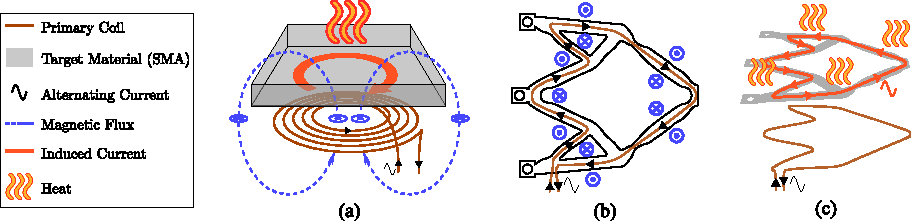
\includegraphics[width=\textwidth]{images/chap5/07_final_schematic_induction.pdf}
  \caption{Induction heating - (a) General principle, (b) 2D view of the coil designed for the deformed inverter, with the direction of the generated magnetic flux normal to the plane, (c) 3D view of the induction system for the inverter problem.}
  \label{fig:induction_schematic}
\end{figure}

When designing the heating solution for maximum induced current, as shown in \cref{eq:back_emf}, a large working frequency is desired. However, when working with alternating currents at high frequencies, undesirable effects such as skin and proximity effects, arise which increase the resistance of the primary coil. Furthermore, the parasitic capacitance of the impedance of the coil will take over above a certain critical frequency, cancelling the inductive effect. By limiting the working frequency, a favourable balance between the losses at the primary coil and the induced current at the resonant value can be maintained. The mutual inductance between the primary coil and the SMA structure can be maximised for a large area of influence and a large number of turns. However, the area of influence cannot be increased as it is constrained by the shape of the generated SMA topology while the number of turns is limited by the associated increase in resistance which in turn reduces the magnitude of the input current. Thus, based on the application, the sizing of the primary coil comes with various trade-offs.

\subsection{Fabrication and Results of Primary Coil}
Due to the complex shape of the generated SMA topologies, the shape of the primary coil must be designed so as to induce a current path across the deformed regions of the compliant mechanism. Currently, the fabrication of the primary coil is performed by hand using nails and a wooden plate. The nails are used to create the shape based on the desired current path and a wire is wound around the nails to fabricate the coil. Once constructed, varnish is used to maintain the shape of the primary coil when the nails are removed. As shown in \cref{fig:induction-coil-freq}, two types of primary coils are constructed using $25$ turns a standard monolithic wire with a copper diameter of $0.30$mm, and another composed of $15$ turns of a Litz wire composed of $300$ strands with a diameter of $0.040$mm each. As shown in \cref{fig:induction-coil-freq}, the resistance of tbe wire increases significantly with the frequency due to the skin and proximity effects. This implies that a thinner effective cross-section is preferred, as in the case of the Litz wire.

As mentioned previously, the working frequency plays an important role in this proposed heating system. A trade-off is present where a higher value increases the heating but also increase the parasitic capacitance of the coil, limiting the impedance above a critical frequency, $\freqCritMONO=17$MHz and $\freqCritLITZ=41$MHz for the coil made of monolithic and Litz wire, respectively. As shown, despite the lower inductance of the Litz coil, better heating performance is achieved due to the working frequency and higher primary current when compared to the monolithic wire.

\begin{figure}[t]
    \centering
    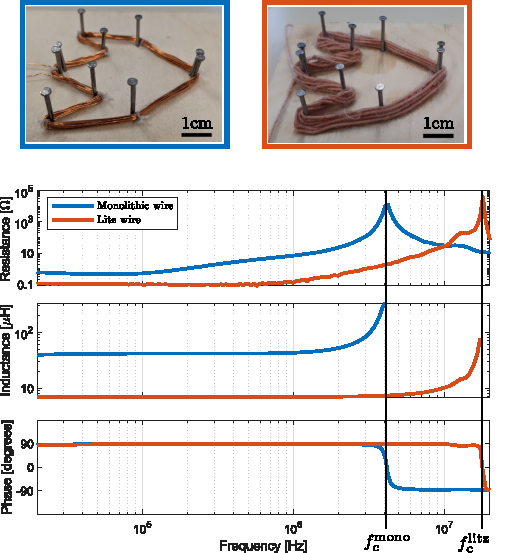
\includegraphics[width=0.75\textwidth]{images/chap5/10_final_Coil_BodeDiagram_2.pdf}
    \caption{Comparison of primary coil with different types of wire. As the impedance becomes mainly capacitive over its critical frequency, the inductance's values after $\freqCritMONO = 17$MHz and $\freqCritLITZ  = 41$MHz are removed for the monolithic and Litz wire respectively.}
    \label{fig:induction-coil-freq}
\end{figure}

Here a working frequency of around $4$ Mhz has been chosen so as to ensure that it sits safely above the critical frequency. At this frequency, the inductance of the coil is $L=7.4~\mu$H and its resistance $R=0.4~\Omega$. A capacitor of $C = 230$ pF is attached in series with the primary coil to create an LC circuit with a resonating frequency $\frequency=(2\pi\sqrt{LC})^{-1} = 3.86$ MHz. Here, the input source is constructed using a half-bridge inverter based on GaN transistors (EPC$9024$). With the Litz coil, a primary current of $I= 1.5$ A is generated at the working frequency while dissipating $0.9$ W of heat. This increased temperature is negligible and implies a stable operation. However, the coil made from the monolithic wire would result in higher temperatures at the primary resulting in a change in resistance and inductance values.

\begin{figure}[t]
    \centering
    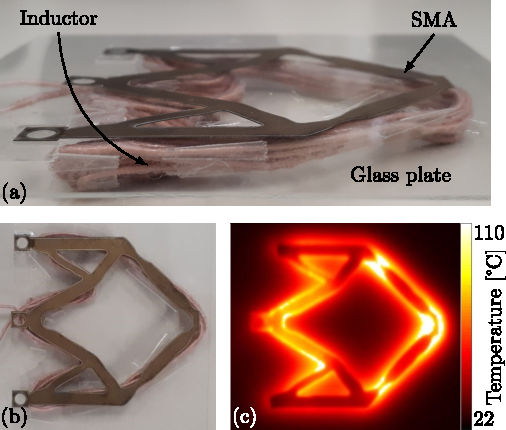
\includegraphics[width=0.75\textwidth]{images/chap5/11_final_results_experiments_heating.pdf}
    % \vspace{-0.3cm}
    \caption{Implementation of induction heating system. When activated, it resulted in the heating of the SMA structure, reverted the deformed structure back to its original shape.}
    \label{fig:induction-heating-temp}
\end{figure}

The \cref{fig:induction-heating-temp} illustrates the implementation of the contactless inductive heating system for the compliant SMA prototype as well as the temperature distribution across the SMA structure using the FLUKE$\textsuperscript \textregistered$ Ti$25$ thermal camera. A glass plate is placed between primary coil and the SMA to avoid any heating through convection. Using the proposed heating system, the SMA inverter prototype was heated above $120^{\circ}$C validating the system as an active heating system. Furthermore, as the structure reverts back to its original shape, this further validates the presence of the shape memory effect.

In this implementation of the prototype, the penetration depth does not limit the excitation frequency as the structure is composed of a thin film of SMA. In the case of a working frequency of $10$ MHz, the penetration depth is larger than the $100~\mu$m thick SMA sheet. However, in a real world application where the compliant structure is created from a thick monolithic block of SMA or 3D printed, the penetration depth would be an additional parameter to account for when sizing the input frequency.

\section{Designing Multi-Output Compliant SMA Actuators}
The proposed design methodology consisting of using topology optimisation to design compliant SMA mechanisms was validated using a FEM simulations and experimental results using standard benchmark problems. Furthermore, as the generative design algorithm used made abstraction of the shape memory effect, the designs of the compliant mechanisms were generated with a relatively low computational time. Due to the cost of NiTiNOL and advanced manufacturing techniques, prototype of the proposed design could not be fabricated but advanced additive manufacturing methods that avoid waste of material such subtractive methods such as machining has become possible as shown in the work by \todocite and \todocite. With these techniques, complex compliant SMA actuators could be fabricated in the near future. Thus, the proposed design methodology could be a great tool in creating novel biased-spring SMA actuators.

\subsection{Generated Multi-Output SMA Actuators}
In this section, various novel multi-output actuators fabricated from compliant SMA topologies are generated based on the proposed design methodology. These topologies were, similar to the benchmark problems in \cref{sec:benchmark-problems}, simulated and their corresponding strain retention factors were measured, as shown in \cref{fig:simo-results}. The \textit{rhombus} structure is a multi-directional mechanism where the axes move in opposing directions. They elongate in the y-axis and contract in the x-axis. The other structures, named the \textit{$8$-point mandrel}, the \textit{$4$-point mandrel $\Xsymbol$} and the \textit{$4$-point mandrel $+$}, perform as outer-mandrels for gripping objects. The evolution of the topology during the generative optimisation process for the \textit{$4$-point mandrel $\Xsymbol$} is shown in \cref{fig:TopologyEvolution-mandrel}. In a similar way to the benchmark problems, these topologies are generated while making abstraction of the shape memory effect and while neglecting the nonlinear nature of the alloy so as to drastically reduce the computational time, which took less than $2$ min per design.
\begin{figure}[hbt!]
    \centering
    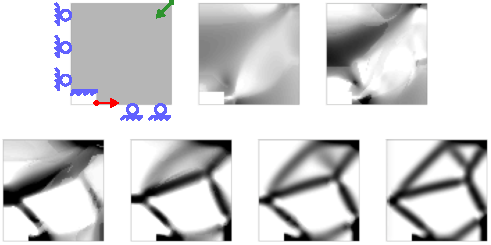
\includegraphics[width=0.7\textwidth]{images/chap5/06_final_evolve_mandrel_2.pdf}
    \caption{$4$-point Mandrel $\Xsymbol$ : Evolution throughout the optimization. The grayscale represents the value of the filtered artificial density. The input force is shown in red and the output force in green.}
    \label{fig:TopologyEvolution-mandrel}
\end{figure}

% \newpage
\begin{figure}[ht!]
    \centering
    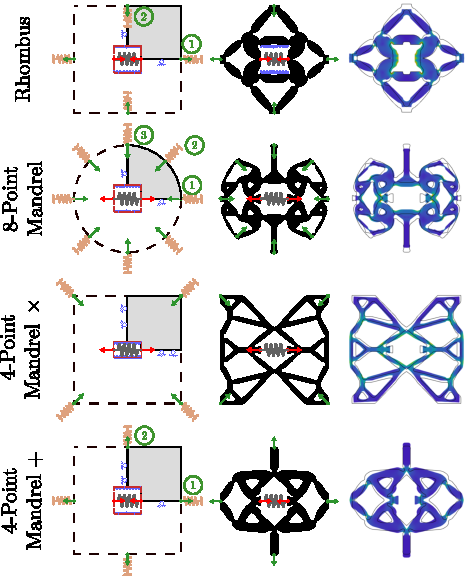
\includegraphics[width=\textwidth]{images/chap5/05_final_SIMO_schematics.pdf}
    \caption{Using the novel design methodology, multi-output bias-spring SMA actuators are generated making use of compliant SMA structures, shown with normalised stress distribution in the deformed state. The input forces are shown in red and the output forces in green. The artificial springs present in the topology optimisation are shown in brown while the bias-springs of the actuators are shown in grey.}
    \label{fig:simo-results}
\end{figure}
% \newpage

Using the FEM simulation of these multi-output compliant mechanisms and the strain retention factor, the presence of the shape memory effect within the generated topologies is validated. A fixed input strain of $10\%$ is applied at each input, where the bias-spring is attached, to have comparable results for each design. The results of the FEM simulation of the design are presented in \cref{tab:simo-results}. The obtained strain retention factor for each actuator topology shows that the majority fo the strain applied by the biasing spring is retained and will be recovered when heated using the proposed induction heating methodology. This implies that this design methodology could be an attractive tool for designing novel multi-output biased-spring SMA actuators.

\begin{table}[hbt!]
    \centering
    \caption{Comparison between the FEM and experimental results of the modified inverter benchmark problem.}
    \label{tab:simo-results}
    % !TEX root = ../sethomas_thesis_main.tex
\documentclass[border=1mm,
               class=article
               preview]{standalone}
\usepackage{tikz}
\begin{document}
\renewcommand{\arraystretch}{1.75}
 \begin{tabular}{P{1.5cm} l l l l c}
 \rowcolor{black} & \textbf{\color{white} $\varepsilon_\text{loaded}^x$}  & \textbf{\color{white} $\varepsilon_\text{loaded}^y$} & \textbf{\color{white} $\varepsilon_\text{free}^x$} & \textbf{\color{white} $\varepsilon_\text{free}^y$} & \textbf{\color{white} $\alpha_\epsilon^x$}\\

 \rowcolor{black!5} & \circled{1} : 0.051 & \circled{1} : 0 & \circled{1} : 0.042 & \circled{1} : 0 & \\
 \rowcolor{black!5} \parbox[t]{2mm}{\multirow{-2}{*}{\rotatebox[origin=c]{90}{Rhombus}}} & \circled{2} : 0 & \circled{2} : 0.062 & \circled{2} : 0 & \circled{2} : 0.045 & \multirow{-2}{*}{\textbf{67.9\%}}\\

  \rowcolor{black!10} & \circled{1} : -0.057 & \circled{1} : 0 & \circled{1} : 0.037 & \circled{1} : 0 & \\
  \rowcolor{black!10} & \circled{2} : -0.057 & \circled{2} : -0.05 & \circled{2} : -0.038 & \circled{2} : -0.034 & \\
  \rowcolor{black!10} \parbox[t]{2mm}{\multirow{-3}{*}{\rotatebox[origin=c]{90}{\makecell{$8$-Point\\Mandrel}}}} & \circled{3} : 0 & \circled{3} : -0.085 & \circled{3} : 0 & \circled{3} : -0.058 & \multirow{-3}{*}{\textbf{74.7\%}}\\

  \rowcolor{black!5} \rule{0pt}{1.25cm}\parbox[t]{2mm}{\rotatebox[origin=c]{90}{\makecell{$4$-Point\\Mandrel $\Xsymbol$}}}  & -0.029 & -0.022 & -0.023 & -0.017 & \textbf{81.4\%}\\[0.75cm]

  \rowcolor{black!10} \rule{0pt}{1cm} & \circled{1} : 0.051 & \circled{1} : 0 & \circled{1} : 0.042 & \circled{1} : 0 & \\
  \rowcolor{black!10} \parbox[t]{2mm}{\multirow{-2}{*}{\rotatebox[origin=c]{90}{\makecell{$4$-Point\\Mandrel $+$}}}} & \circled{2} : 0 & \circled{2} : 0.062 & \circled{2} : 0 & \circled{2} : 0.045 & \multirow{-2}{*}{\textbf{68\%}}\\[0.5cm]
\end{tabular}
% }
\renewcommand{\arraystretch}{1}
\end{document}

\end{table}

\section{Kirigami inspired Compliant SMA Actuators}
Using topology optimization, various compliant SMA actuators can be designed with the intent to combine the functions of the kinematic stage and the active element. However, due to the current limitations of fabrication and its costs, the feasibility of such an actuator, in the current sense, is unlikely. As additive manufacturing of SMAs becomes more accessible, the advantages of designing compliant SMA structures such as increasing the overall work density of the actuator, will become more apparent and attractive.

Kirigami, the Japanese art of cutting paper to create intricate structure, has gained traction in various engineering fields to create stretchable structure as shown in the work by \todocite. While designing 3D compliant structure made of SMA is expensive, this kirigami approach can be extended to SMAs to create compliant structures that when cut in a specific manner, can exhibit surprising mechanical behaviours.

When designing actuators, a key detail to keep in mind is the life cycle of the device. In common industrial applications, the number of cycles to fatigue of traditional grippers can exceed $10^6$ cycles. In the case of SMA actuators, this number is much lower and is directly related to the structural fatigue of the material. The determining factors regarding the fatigue life of SMAs are the strain amplitude and the type of strain applied to the material. The work by \cite{runcimanEquivalentStrainCoffin2011} looks at the fatigue lifetime of NiTiNOL based on different loading conditions, such as torsion, tension and bending. They conclude that SMAs tend to have a much longer life cycle when loading under torsion or bending when compared to tension. The results show that with a fixed strain amplitude of 1\%, in tension, the number of cycles to failure is less than $10^3$ whereas in bending or torsion, the number of cycles to failure is around $10^5$.

The availability of NiTiNOL in different geometries such as springs, wires and sheets, has allowed the creation of multiple classes of SMA actuators that exploit their respective advantages. As mentioned in previous sections, the simplest approach would be to use the alloy in the shape of a wire paired with a biasing spring to drive an actuator where the stress and strain of the material corresponds directly to the stroke and force output of the actuator. In these cases, SMA wires are elongated under pure traction and are then heated to recover the strain and provide the force output as shown in the works by \cite{kyungDesignMicrogripperMicromanipulation2008}, \cite{welschVacuumGripperSystem2018}, \cite{haibinModelingGraspingForce2018}, and \cite{andrianesisDevelopmentControlMultifunctional2015}. Here, the stroke of the actuator can not exceed 1\% without compromising its fatigue life. Thus, in cases where a larger stroke is required, the geometry of the wire is adapted to form a spring which can provide stroke above 100\% as implemented in the works by \cite{ikutaMicroMiniatureShape1990} and \cite{zhakypovOrigamiInspiredReconfigurableSuction2018}. Here, the material no longer deforms in traction but rather in torsion, thereby increasing its fatigue life but while compromising the force output. This implies that there is a trade-off to be made between the force output, and the stroke and fatigue life.

Since SMAs are available in the form of sheets which can be machined using laser cutters into complex geometries, different kinds of SMA actuator systems exploit the longer fatigue life of SMAs in flexion to create novel grippers as shown in the works by \cite{kohlSMAMicrogripperSystem2002}, \cite{benardThinfilmShapememoryAlloy1998}, \cite{zhakypovOrigamiInspiredReconfigurableSuction2018}. The major advantage to using sheets instead of wires is the fact that they provide a much higher force output. The difference in force output between sheets and wires can be reduced by placing multiple wires in parallel to generate forces in the same order of magnitude as sheets. Thus in applications, where a higher force output is required, the use of SMA sheets or multiple wires in parallel can be a viable solution.

When working with thin wires, placing them in parallel to augment the overall force output also increases the complexity of the system greatly. The manufacturing and assembly of such a system can be difficult. Furthermore, it is also impossible to uniformly deform all the wires equally, resulting in some wires being inactive during the shape memory effect. Thus, in cases where a higher force output is required, the design space can become limited to just using sheets. For maximum force output, the sheet can be elongated in pure traction but only up to about 1\%. In applications where a large stroke and force output is required, the SMA sheets in its original state is no longer viable. Traditionally, this limitation is overcome by adding a kinematic stage to amplify the stroke of the SMA actuator but comes with the cost of reduced overall work density of the final actuator.

In this section, a novel approach will look at a new kirigami-based approach to designing SMA sheets to obtain an actuator that can provide higher force output while being able to also provide high strokes. Kirigami is a variation of origami that involves the cutting of the substrate to create different shapes and behaviours. The pattern presented in this paper is based on the work by \cite{shyuKirigamiApproachEngineering2015} where a nanocomposite substrate is patterned to create a stretchable element. This approach allows an SMA sheet to reach strains over 100\% without losing its capacity to deliver a high force output.

\subsection{Proposed Patterns}
\subsection{Implementation}

\section{Summary and Conclusion}
In this chapter, a design methodology, consisting of integrating the kinematic stage and active element to create a compact SMA actuator, is proposed. Using topology optimization and a novel approach to generate topologies while making abstraction of the shape memory effect is detailed. By implementing such a generative algorithm, the computational time to design novel topologies has been drastically reduced. This has the implication to extending such a design algorithm to 3D structures.

The design approach using topology optimisation was tested using benchmark problems with a standard input and output parameters to create various topologies that can be fabricated from SMAs. The presence of the shape memory effect and the feasibility of the topologies to be used in SMA actuators was validated using a FEM simulation and an experimental prototype. Furthermore, a qualitative measure called the strain retention factor was proposed as a means to compare the various topologies that can be generated using such an approach.

As these novel structures can be complex, the heating of such geometries using simple Joule's heating is no longer trivial. A novel heating solution was proposed and fabricated so as to activate the shape memory effect of the fabricated topologies. Furthermore, using this design approach and generative design algorithm, various multi-output biased-spring SMA actuators, that can be actuated using only a single biasing spring, were proposed.

These SMA structures were designed within a 2D space with the intention of fabricating the structure from a 3D monolithic block of SMA. As the design algorithm was implemented with a volume constraint to preserve material, fabricating the structure with subtractive methods such as machining will result in large amounts of wasted material. However, due to the current cost limitations of additive manufacturing processes that exist for SMA, the feasibility of such a compliant SMA structure is limited.

Lastly, the same methodology where structure composed of complex patterns that exhibit surprising mechanical behaviours, can be be seen in kirigami-inspired structures. By extending this same design principle to SMA actuators, patterns can be cut into thin SMA sheets such that high stroke actuators can be fabricated without the need for cumbersome external kinematic stages.

Using this design principle, compliant SMA active elements can be designed and fabricated so as to appropriate the functions of the kinematic stage within the SMA actuator. This allows for the creation of compact SMA actuators that retain their high work energy density.
